%\documentclass{article}
\documentclass[a4paper,twoside]{book} %this has problems
%
% loading packages
%

\RequirePackage{ifpdf}
\RequirePackage{ifxetex}

%
%
\ifpdf
  \RequirePackage[pdftex,%
       bookmarksnumbered,%
              colorlinks,%
          linkcolor=blue,%
              hyperindex,%
        plainpages=false,%
       pdfstartview=FitH]{hyperref}
\else\ifxetex
  \RequirePackage[bookmarksnumbered,%
               colorlinks,%
           linkcolor=blue,%
               hyperindex,%
         plainpages=false,%
        pdfstartview=FitH]{hyperref}
\else
  \RequirePackage[dvipdfm,%
        bookmarksnumbered,%
               colorlinks,%
           linkcolor=blue,%
               hyperindex,%
         plainpages=false,%
        pdfstartview=FitH]{hyperref}
\fi\fi
%\usepackage{hyperref}

% other packages
%--------------------------------------------------------------------------
\usepackage{graphicx, color}
\usepackage{subfig}
\usepackage{tikz}
\usetikzlibrary{matrix,positioning}

\usepackage{amsmath, amsthm, amssymb} % for math
\usepackage{exercise} % for exercise
\usepackage{import} % for nested input

%
% for programming
%
\usepackage{verbatim}
\usepackage{listings}
%\usepackage{algorithmic} %old version; we can use algorithmicx instead
\usepackage{algorithm}
\usepackage[noend]{algpseudocode} %for pseudo code, include algorithmicsx automatically
\usepackage{appendix}
\usepackage{makeidx} % for index support
\usepackage{titlesec}

\titleformat{\paragraph}
{\normalfont\normalsize\bfseries}{\theparagraph}{1em}{}
\titlespacing*{\paragraph}
{0pt}{3.25ex plus 1ex minus .2ex}{1.5ex plus .2ex}

\lstdefinelanguage{Smalltalk}{
  morekeywords={self,super,true,false,nil,thisContext}, % This is overkill
  morestring=[d]',
  morecomment=[s]{"}{"},
  alsoletter={\#:},
  escapechar={!},
  literate=
    {BANG}{!}1
    {UNDERSCORE}{\_}1
    {\\st}{Smalltalk}9 % convenience -- in case \st occurs in code
    % {'}{{\textquotesingle}}1 % replaced by upquote=true in \lstset
    {_}{{$\leftarrow$}}1
    {>>>}{{\sep}}1
    {^}{{$\uparrow$}}1
    {~}{{$\sim$}}1
    {-}{{\sf -\hspace{-0.13em}-}}1  % the goal is to make - the same width as +
    %{+}{\raisebox{0.08ex}{+}}1		% and to raise + off the baseline to match -
    {-->}{{\quad$\longrightarrow$\quad}}3
	, % Don't forget the comma at the end!
  tabsize=2
}[keywords,comments,strings]

% for better Haskell code outlook
\lstdefinelanguage{Haskell}{
  basicstyle=\small\ttfamily,
  flexiblecolumns=false,
  basewidth={0.5em,0.45em},
  literate={+}{{$+$}}1 {/}{{$/$}}1 {*}{{$*$}}1 {=}{{$=$}}1
           {>}{{$>$}}1 {<}{{$<$}}1 {\\}{{$\lambda$}}1
           {\\\\}{{\char`\\\char`\\}}1
           {->}{{$\rightarrow$}}2 {>=}{{$\geq$}}2 {<-}{{$\leftarrow$}}2
           {<=}{{$\leq$}}2 {=>}{{$\Rightarrow$}}2
           {\ .}{{$\circ$}}2 {\ .\ }{{$\circ$}}2
           {>>}{{>>}}2 {>>=}{{>>=}}2
           {|}{{$\mid$}}1
}[keywords,comments,strings]

\lstloadlanguages{C, C++, Lisp, Haskell, Python, Smalltalk}

\lstset{
  showstringspaces = false
}

% ======================================================================

\def\BibTeX{{\rm B\kern-.05em{\sc i\kern-.025em b}\kern-.08em
    T\kern-.1667em\lower.7ex\hbox{E}\kern-.125emX}}

%
% mathematics
%
\newcommand{\be}{\begin{equation}}
\newcommand{\ee}{\end{equation}}
\newcommand{\bmat}[1]{\left( \begin{array}{#1} }
\newcommand{\emat}{\end{array} \right) }
\newcommand{\VEC}[1]{\mbox{\boldmath $#1$}}

% numbered equation array
\newcommand{\bea}{\begin{eqnarray}}
\newcommand{\eea}{\end{eqnarray}}

% equation array not numbered
\newcommand{\bean}{\begin{eqnarray*}}
\newcommand{\eean}{\end{eqnarray*}}

\newtheorem{theorem}{Theorem}[section]
\newtheorem{lemma}[theorem]{Lemma}
\newtheorem{proposition}[theorem]{Proposition}
\newtheorem{corollary}[theorem]{Corollary}


\setcounter{page}{1}

% ==================== Book flag==========================

\global\let\wholebook=\relax %without relax, we build article, esle book

\graphicspath{
	{img/}
        {others/preface/}
	{datastruct/tree/binary-search-tree/}
        {sorting/insertion-sort/}
	{datastruct/tree/red-black-tree/}
        {datastruct/tree/AVL-tree/}
	{datastruct/tree/trie/}
        {datastruct/tree/suffix-tree/}
        {datastruct/tree/B-tree/}
        {datastruct/heap/binary-heap/}
        {datastruct/heap/other-heaps/}
        {datastruct/elementary/queue/}
        {datastruct/elementary/sequence/}
        {others/appendix/list/}
}

\makeindex

\begin{document}

% set PDF properties
\hypersetup{pdftitle={algoxy},%
            pdfauthor={liuxinyu95@gmail.com},%
            pdfsubject={Computer Science},%
            pdfkeywords={Algorithm, Programming}}

% ================================================================
%                 COVER PAGE
% ================================================================

\title{{\bf \Huge AlgoXY} elementary algorithms
  %\scalebox{1.2}{\includegraphics{images/clouds.eps}}
            }

\author{Liu Xinyu
  \thanks{{\bfseries Liu Xinyu } \newline
    Draft version 2012, Beijing \newline
    Email: liuxinyu95@gmail.com \newline
    }}

\maketitle

% ================================================================
%                 Content
% ================================================================

%\newpage
\tableofcontents
\newpage

%\part{Introduction}
\ifx\wholebook\relax \else
% ------------------------

\documentclass[b5paper]{article}

\usepackage[en]{../../prelude}

\setcounter{page}{1}

\begin{document}

\title{Preface}

\author{Xinyu LIU
\thanks{{\bfseries Xinyu LIU} \newline
  Email: liuxinyu95@gmail.com \newline}
  }

\maketitle
\fi

\markboth{Preface}{Elementary Algorithms}

\chapter*{Preface}
\phantomsection  % so hyperref creates bookmarks
\addcontentsline{toc}{chapter}{Preface}

Programmers learn elementary algorithms at school. Except for programming contest or code interview, they seldom develop algorithms at work. Most time, the needed algorithms or data structures are provided in libraries. We needn't bother to `re-invent the wheel'. When talking about algorithms in AI and machine learning, people actually mean scientific modeling. Elementary algorithms are fundamental things, Let's start with two puzzles.

\section*{The smallest free number}
\label{min-free} \index{minimum free number}

Richard Bird gives a problem to find the minimum number that not appears in a list (Chapter 1, \cite{fp-pearls}). People use number to index entities. A number is either occupied or free. When acquire, we always want to allocate the smallest available one. Suppose numbers are non-negative integers and those being used are recorded in a list, for example:

\begin{Verbatim}[fontsize=\footnotesize]
[18, 4, 8, 9, 16, 1, 14, 7, 19, 3, 0, 5, 2, 11, 6]
\end{Verbatim}

How can we find the smallest free number, 10, from this list? It seems quite easy with exhaustive search:

\begin{algorithmic}[1]
\Function{Min-Free}{$A$}
  \State $x \gets 0$
  \Loop
    \If{$x \notin A$}
      \State \Return $x$
    \Else
      \State $x \gets x + 1$
    \EndIf
  \EndLoop
\EndFunction
\end{algorithmic}

Where the $\notin$ is realized as below.

\begin{algorithmic}[1]
\Function{`$\notin$'}{$x, X$}
  \For{$i \gets 1 $ to $|X|$}
    \If{$x = X[i]$}
      \State \Return False
    \EndIf
  \EndFor
  \State \Return True
\EndFunction
\end{algorithmic}

Where $|X| = n$ is the length of $X$. Some environments have built-in implementation to test existence of an element. However, this solution performs poor with millions of numbers. The time spent is quadratic to $n$. In a computer with 2 cores of 2.10 GHz CPU, and 2G RAM, the C implementation takes 5.4s to find the answer among 100K numbers, and exceeds 8 minutes to handle 1 million numbers.

\subsection*{Improvement}
For $n$ numbers $x_1, x_2, ..., x_n$, if there is a free number, some $x_i$ must be out of the range $[0, n)$\footnote{Range $[a, b)$ starts from $a$ to $b$, but excludes $b$.}; otherwise the list is exactly some permutation of $0, 1, ..., n - 1$ hence $n$ is the minimum free number.

\be
\textit{minfree}(x_1, x_2, ..., x_n) \leq n
\label{eq:min-free}
\ee

We use an array $F$ of $n + 1$ flags to mark whether a number is free in $[0, n]$.

\begin{algorithmic}[1]
\Function{Min-Free}{$A$}
  \State $F \gets $[False, False, ..., False] \Comment{$n+1$}
  \For{$x$ in $A$}
    \If{$x < n$}
      \State $F[x] \gets$ True
    \EndIf
  \EndFor
  \For{$i \gets 0$ to $n$}
    \If{$F[i] =$ False}
      \State \Return $i$
    \EndIf
  \EndFor
\EndFunction
\end{algorithmic}

Initialize $F$ with all False values. For every number $x$ in $A$, mark the flag $F[x]$ true if $x < n$. Finally, scan $F$ to find the first false flag. This program takes time proportion to $n$. It uses $n + 1$ flags to cover the special case that $sort(A) = [0, 1, 2, ..., n-1]$. To avoid repeated allocate then release the flags, we can pre-allocate a sufficient big buffer for reusing, and change to bit-wise flags instead of array. The C implementation handles 1 million numbers in 0.023s in the same computer.

%% \begin{lstlisting}[language=C]
%% #define N 1000000
%% #define WORD_LENGTH (sizeof(int) * 8)

%% void setbit(unsigned int* bits, unsigned int i) {
%%     bits[i / WORD_LENGTH] |= 1 << (i % WORD_LENGTH);
%% }

%% int testbit(unsigned int* bits, unsigned int i) {
%%     return bits[i / WORD_LENGTH] & (1 << (i % WORD_LENGTH));
%% }

%% unsigned int bits[N / WORD_LENGTH + 1];

%% int minfree(int* xs, int n) {
%%   int i, len = N/WORD_LENGTH + 1;
%%   for (i = 0; i < len; ++i) {
%%       bits[i]=0;
%%   }
%%   for (i=0; i < n; ++i) {
%%       if(xs[i] < n) {
%%           setbit(bits, xs[i]);
%%       }
%%   }
%%   for (i=0; i <= n; ++i) {
%%       if (!testbit(bits, i)) {
%%           return i;
%%       }
%%   }
%% }
%% \end{lstlisting}

\subsection*{Divide and Conquer}
The divide and conquer method breaks the problem into smaller ones, then solve them and consolidate the result. Collect $x_i \leq \lfloor n/2 \rfloor$ in sub-list $A'$ and the rest in another $A''$. According to \cref{eq:min-free}, if the length of $|A'| = \lfloor n/2 \rfloor$, it means $A'$ is `full'. The minimum free number must be in $A''$, otherwise in $A'$. Both cases lead to a smaller problem. When search in $A''$, we start from $\lfloor n/2 \rfloor + 1$, but not from $0$. We define the algorithm as $search(A, l, u)$, where $l$ and $u$ are the lower and upper bounds. We start from $minfree(A) = search(A, l = 0, u = |A|-1)$:

\[
\begin{array}{rcl}
search(\nil, l, u) & = & l \\
search(A, l, u) & = & \begin{cases}
       |A'| = m - l + 1 : & search(A'', m+1, u) \\
       otherwise : & search(A',  l, m) \\
\end{cases}
\end{array}
\]

where:

\[
\begin{cases}
m = \lfloor \dfrac{l + u}{2} \rfloor \\
A' = [x \leq m, x \in A], A'' = [x > m, x \in A] \\
\end{cases}
\]

This algorithm needn't additional space\footnote{The recursion takes $O(\lg n)$ stack spaces, but it can be eliminated through tail recursion optimization}. Each recursive call performs $O(|A|)$ comparisons to partition $A'$ and $A''$, hence halves the problem as $T(n) = T(n/2) + O(n)$. We can reduce it to $O(n)$ according to the master theorem\footnote{Alternatively, the first call takes $O(n)$ time to partition $A'$ and $A''$, the second call takes $O(n/2)$ time, the third call takes $O(n/4)$ time ... The total time is $O(n + n/2 + n/4 + ...) = O(2n) = O(n)$.}. Below example program implements this algorithm.

\lstset{frame = single}
\begin{Haskell}
minFree xs = bsearch xs 0 (length xs - 1)

bsearch xs l u | xs == [] = l
               | length as == m - l + 1 = bsearch bs (m + 1) u
               | otherwise = bsearch as l m
    where
      m = (l + u) `div` 2
      as = [x | x <- xs, x <= m]
      bs = [x | x <- xs, x > m]
\end{Haskell}

There are $O(\lg n)$ recursive calls. We can eliminate the recursion with loops:

\begin{algorithmic}[1]
\Function{Min-Free}{$A$}
  \State $l \gets 0, u \gets |A|$
  \While{$u - l > 0$}
    \State $m \gets \lfloor \dfrac{u + l}{2} \rfloor$
    \State $left \gets l$
    \For{$right \gets l$ to $u - 1$}
      \If{$A[right] \leq m$}
        \State Exchange $A[left] \leftrightarrow A[right]$
        \State $left \gets left + 1$
      \EndIf
    \EndFor
    \If{$left < m + 1$}
      \State $u \gets left$
    \Else
      \State $l \gets left$
    \EndIf
  \EndWhile
\EndFunction
\end{algorithmic}

As shown in \cref{fig:divide}, this program re-arranges the array such that all elements before $left$ are less than or equal to $m$; while those between $left$ and $right$ are greater than $m$.

\begin{figure}[htbp]
  \centering
  \includegraphics[scale=0.7]{img/partition-by}
  \caption{All $A[i] \leq m$ where $0 \leq i < left$; while $A[i] > m$ where $left \leq i < right$. The rest are yet to be scanned.}
  \label{fig:divide}
\end{figure}

\section*{Regular number}

The second problem is to find the 1,500-th number, which only contains factor 2, 3 or 5. Such numbers are called the regular numbers\footnote{Also known as 5-smooth numbers in number theory, and Hamming numbers named after Richard Hamming.}. 2, 3, and 5 are definitely regular numbers. $60 = 2^23^15^1$ is the 25-th regular number. $21 = 2^03^17^1$ is not because it has a factor of 7. Define $1=2^03^05^0$ as the 0-th regular number. The first 10 are:

1, 2, 3, 4, 5, 6, 8, 9, 10, 12, ...

\subsection*{The brute-force solution}
We can check numbers one by one from 1, extract all factors of 2, 3 and 5 to see if the remaining is 1:

\begin{algorithmic}[1]
\Function{Regular-Number}{$n$}
  \State $x \gets 1$
  \While{$n > 0$}
    \State $x \gets x + 1$
    \If{\Call{Valid?}{$x$}}
      \State $n \gets n - 1$
    \EndIf
  \EndWhile
  \State \Return $x$
\EndFunction
\Statex
\Function{Valid?}{$x$}
  \While{$x \bmod 2 = 0$}
    \State $x \gets x / 2$
  \EndWhile
  \While{$x \bmod 3 = 0$}
    \State $x \gets x / 3$
  \EndWhile
  \While{$x \bmod 5 = 0$}
    \State $x \gets x / 5$
  \EndWhile
  \State \Return $x = 1$ ?
\EndFunction
\end{algorithmic}

This `brute-force' algorithm performs poor when $n$ increases. The C implementation takes 40.39s in above computer to find the 1500-th number (860934420).

\subsection*{Improvement}
Modular and divide are expensive operations\cite{Bentley}. Instead of checking every number, we can generate regular numbers from 1 in ascending order. We use a queue, which allows to add number to one end (enqueue), and remove from the other end (dequeue). The number enqueued first will be dequeued first (First In First Out). Initialize the queue with 1, the 0th regular number. We repeatedly dequeue a number, multiply it by 2, 3, 5 to generate 3 new numbers; then add them to the queue in ascending order. We drop the number if it is already in the queue, as shown in \cref{fig:queues}.

\begin{figure}[htbp]
  \centering
  \includegraphics[scale=0.5]{img/regular-num-1q}
  \caption{First 4 steps.}
  \label{fig:queues}
\end{figure}

\begin{algorithmic}[1]
\Function{Regular-Number}{$n$}
  \State $Q \gets [1]$
  \While{$n > 0$}
    \State $x \gets$ \Call{Dequeue}{$Q$}
    \State \Call{Unique-Enqueue}{$Q, 2x$}
    \State \Call{Unique-Enqueue}{$Q, 3x$}
    \State \Call{Unique-Enqueue}{$Q, 5x$}
    \State $n \gets n-1$
  \EndWhile
  \State \Return $x$
\EndFunction
\Statex
\Function{Unique-Enqueue}{$Q, x$}
  \State $i \gets 0, m \gets |Q|$
  \While{$i < m$ and $Q[i] < x$}
    \State $i \gets i + 1$
  \EndWhile
  \If{$i \geq m$ or $x \neq Q[i]$}
    \State \Call{Insert}{$Q, i, x$}
  \EndIf
\EndFunction
\end{algorithmic}

The \textproc{Unique-Enqueue} function takes $O(m)$ time to uniquely insert a number in ascending order, where $m = |Q|$ is the length of the queue. It increases proportion to $n$ (Each time, we dequeue an element, and enqueue at most 3. The increasing ratio $\leq$ 2), the total time is $O(1 + 2 + 3 + ... + n) = O(n^2)$. \Cref{fig:big-O-1q} shows the queue access times against $n$. The quadratic curve reflects the $O(n^2)$ performance.

\begin{figure}[htbp]
  \centering
  \includegraphics[scale=0.5]{img/big-O-1q}
  \caption{Queue access count - $n$.}
  \label{fig:big-O-1q}
\end{figure}

The corresponding C implementation takes 0.016s to output 860934420, about 2500 times faster than the brute-force solution. Let $xs = [x_1, x_2, x_3, ...]$ be the infinite list of all regular numbers. Multiply every number by 2, the result is again infinite many regular numbers: $[2x_1, 2x_2, 2x_3, ...]$, so as multiply by 3 and 5. If we merge the three infinite lists together, filter out the duplicated numbers, and prepend 1 as the first, we get $xs$ again:

\be
  xs = 1 : [2x | x \gets xs] \cup [3x | x \gets xs] \cup [5x | x \gets xs]
\ee

Where $x \cons xs$ links $x$ before list $xs$. It is called `cons' in Lisp. 1 is linked as the head (the 0th regular number). $\cup$ merges two lists:

\[
(a \cons as) \cup (b \cons bs) = \begin{cases}
  a < b: & a : as \cup (b \cons bs) \\
  a = b: & a : as \cup bs \\
  a > b: & b : (a \cons as) \cup bs \\
\end{cases}
\]

Below is the example program:

\begin{Haskell}
xs = 1 : [2*x | x <- xs] `merge` [3*x | x <- xs] `merge` [5*x | x <- xs]

merge (a:as) (b:bs) | a < b = a : merge as (b:bs)
                    | a == b = a : merge as bs
                    | otherwise = b : merge (a:as) bs
\end{Haskell}

This example program gives the 1500th number 860934420 by \texttt{xs !! 1500} in 0.03s in the same computer.

\subsection*{Queues}
The above solution needs filter out duplicated numbers, scan the queue to maintain the ascending order. We category all regular numbers into 3 disjoint buckets: $Q_2 = \{2^i | i > 0\}$, $Q_{23} = \{ 2^i3^j | i \geq 0, j > 0 \}$, and $Q_{235} = \{ 2^i3^j5^k | i,j \geq 0, k > 0\}$. Constraint $j \neq 0$ in $Q_{23}$, and $k \neq 0$ in $Q_{235}$ such there is no overlap. Realize the buckets as 3 queues starting from $Q_2 = \{ 2 \}$, $Q_{23} = \{ 3\}$, and $Q_{235} = \{ 5 \}$. Each time extract the smallest $x$ from the queues, then do the following:

\begin{itemize}
\item If $x$ comes from $Q_2$, enqueue $2x$ to $Q_2$, $3x$ to $Q_{23}$, and $5x$ to $Q_{235}$;
\item If $x$ comes from $Q_{23}$, enqueue $3x$ to $Q_{23}$, and $5x$ to $Q_{235}$. We do not add $2x$ to $Q_2$, because $Q_2$ does not hold any numbers divisible by 3.
\item If $x$ comes from $Q_{235}$, enqueue $5x$ to $Q_{235}$. We do not add $2x$ to $Q_2$, or $3x$ to $Q_{23}$ because they don't hold numbers divisible by 5.
\end{itemize}

We reach to the answer after dequeue $n$ numbers. \Cref{fig:q235} gives the first 4 steps.

\begin{figure}[htbp]
  \centering
  \includegraphics[scale=0.5]{img/q235}
  \caption{First 4 steps with $Q_2$, $Q_{23}$, and $Q_{235}$.}
  \label{fig:q235}
\end{figure}

\begin{algorithmic}[1]
\Function{Regular-Number}{$n$}
  \State $x \gets 1$
  \State $Q_2 \gets \{ 2 \}$, $Q_{23} \gets \{ 3 \}$, $Q_{235} \gets \{ 5 \}$
  \While{$n > 0$}
    \State $x \gets min$(\Call{Head}{$Q_2$}, \Call{Head}{$Q_{23}$}, \Call{Head}{$Q_{235}$})
    \If{$x =$ \Call{Head}{$Q_2$}}
      \State \Call{Dequeue}{$Q_2$}
      \State \Call{Enqueue}{$Q_2, 2x$}
      \State \Call{Enqueue}{$Q_{23}, 3x$}
      \State \Call{Enqueue}{$Q_{235}, 5x$}
    \ElsIf{$x=$ \Call{Head}{$Q_{23}$}}
      \State \Call{Dequeue}{$Q_{23}$}
      \State \Call{Enqueue}{$Q_{23}, 3x$}
      \State \Call{Enqueue}{$Q_{235}, 5x$}
    \Else
      \State \Call{Dequeue}{$Q_{235}$}
      \State \Call{Enqueue}{$Q_{235}, 5x$}
    \EndIf
    \State $n \gets n - 1$
  \EndWhile
  \State \Return $x$
\EndFunction
\end{algorithmic}

This algorithm loops $n$ times. Each time extracts the minimum number in constant time. Then adds at most 3 numbers to the queues in constant time. The overall performance is $O(n)$.

\section*{Summary}
Both brute-force solutions can't scale up. This book is {\em not} about coding contest or code interview, but aims to provide both purely functional algorithms and their counterpart imperative implementations. We referenced many results from Okasaki's work\cite{okasaki-book} and classic text books\cite{CLRS}. We avoid relying on a specific programming language, because the reader may or may not be familiar with it, and programming languages keep changing. Instead, we use pseudo code or mathematics notation to make the algorithm definition generic. When give code examples, the functional ones look more like Haskell, and the imperative ones look like a mix of several languages.

I wrote the first edition from 2009 to 2017, then rewrote the second edition and added answers to the 119 exercises from 2020 to 2023. The pdf can be downloaded from github.

\begin{Exercise}\label{ex:preface}
\Question{For the free number puzzle, since all numbers are not negative, we can reuse the sign as a flag. For every $|x| < n$ (where $n$ is the length), negate the number at position $|x|$. Then scan to find the first positive number. Its position is the answer. Write a program to realize this solution.}

\Question{There are $n$ numbers 1, 2, ..., $n$. After some processing, they are shuffled, and a number $x$ is altered to $y$. Suppose $1 \leq y \leq n$, design a solution to find $x$ and $y$ in linear time with constant space.}

\Question{Below example program is a solution for the regular number puzzle. Is it equivalent to the queue based solution?
\begin{lstlisting}[language = Bourbaki]
Int regularNum(Int m) {
    [Int] nums(m + 1)
    Int n = 0, i = 0, j = 0, k = 0
    nums[0] = 1
    Int x2 = 2 * nums[i]
    Int x3 = 3 * nums[j]
    Int x5 = 5 * nums[k]
    while n < m {
        n = n + 1
        nums[n] = min(x2, x3, x5)
        if x2 == nums[n] {
            i = i + 1
            x2 = 2 * nums[i]
        }
        if x3 == nums[n] {
            j = j + 1
            x3 = 3 * nums[j]
        }
        if x5 == nums[n] {
            k = k + 1
            x5 = 5 * nums[k]
        }
    }
    return nums[m]
}
\end{lstlisting}
}
\end{Exercise}

\begin{Answer}[ref={ex:preface}]
\Question{For the free number puzzle, since all numbers are not negative, we can reuse the sign as a flag. For every $|x| < n$ (where $n$ is the length), negate the number at position $|x|$. Then scan to find the first positive number. Its position is the answer. Write a program to realize this solution.

\begin{Bourbaki}
Int minFree([Int] nums) {
    var n = length(nums)
    for Int i = 0 to n - 1 {
        var k = abs(nums[i])
        if k < n then nums[k] = -abs(nums[k])
    }
    for Int i = 0 to n - 1 {
        if nums[i] > 0 then return i
    }
    return n
}
\end{Bourbaki}
}

\Question{There are $n$ numbers 1, 2, ..., $n$. After some processing, they are shuffled, and a number $x$ is altered to $y$. Suppose $1 \leq y \leq n$, design a solution to find $x$ and $y$ in linear time with constant space.

For example $X$ = [3, 1, 3, 5, 4], the missing number $x = 2$, the duplicated one $y = 3$. We give 4 methods: (1) divide and conquer; (2) pigeon hole sort; (3) sign encoding; and (4) equations.

\textbf{Divide and conquer}: Partition the numbers with the middle point $m = \lfloor \dfrac{1 + n}{2} \rfloor$: the left $as = [a \leq m, a \gets X]$, and the right $bs = [b > m, b \gets X]$. If the length of $|as| < m$, then the missing number is on the left, let $s = 1 + 2 + ... + m = \dfrac{m (m + 1)}{2}$, then $x = s - sum(as)$. We can also calculate the missing one on the right. Let $s' = (m + 1) + (m + 2) + ... + n = \dfrac{(n + m + 1)(n - m)}{2}$, then $y = sum(bs) - s'$. If the length of $|as| > m$, then the duplicated number is on the left. Use the similar method, we calculate the missing number $x = s' - sum(bs)$, and the duplicated number $y = sum(as) - s$. Otherwise if the length $|as| = m$, then there are $m$ numbers not greater than $m$. But we don't know whether they are some permutation of 1, 2, ..., $m$. We can calculate and compare $sum(as)$ and $s$. If equal, then we can drop all numbers on the left, then recursively find $x$ and $y$ on the right; otherwise, we drop the right, recursively find on the left. In recursive finding, we need replace the lower bound of 1 with $l$. Because we halve the list every time, the overall performance is $O(n)$ according to the master theorem.

\begin{Haskell}
missDup xs = solve xs 1 (length xs) where
  solve xs@(_:_:_) l u | k < m - l + 1 = (sl - sl', sr' - sr)
                       | k > m - l + 1 = (sr - sr', sl' - sl)
                       | sl == sl' = solve bs (m + 1) u
                       | otherwise = solve as l m
      where
          m = (l + u) `div` 2
          (as, bs) = partition (<=m) xs
          k = length as
          sl = (l + m) * (m - l + 1) `div` 2
          sr = (m + 1 + u) * (u - m) `div` 2
          (sl', sr') = (sum as, sum bs)
\end{Haskell}

\textbf{Pigeon hole sort}. Since all numbers are within the range from 1 to $n$, we can do pigeon hole sort. Scan from left to right, for every number $x$ at position $i$, if $x \neq i$, we swap it with number $y$ at position $x$. We find the duplicated number if $x = y$, besides, we find the missing number $i$. Repeat this till $x = i$ or meet the duplicated number. Because every number is swapped to its right position a time, the total performance is $O(n)$.

\begin{Bourbaki}
(Int, Int) missDup([Int] xs) {
    Int miss = -1, dup = -1
    for Int i = 0 to length(xs) - 1 {
        while xs[i] != i {
            Int j = xs[i]
            if xs[j] == xs[i] {
                dup = xs[j]
                miss = i
                break
            } else {
                j = xs[i]
                (xs[i], xs[j]) = (xs[j], xs[i])
            }
        }
    }
    return (miss, dup)
\end{Bourbaki}

\textbf{Sign encoding}. Setup an array of $n$ flags. For every number $x$, mark the $x$-th flag in the array true. When meet the duplicated number, the corresponding flag was marked before. Let the duplicated number be $d$, we know $s = 1 + 2 + ... + n = \dfrac{n (n + 1)}{2}$, and the sum $s'$ of all numbers. We can calculate the missing number $m = d + s - s'$. However, this method need additional $n$ flags. The existence of a number is a type of binary information (yes/no), we can encode it as the positive/negative sign, hence re-use the space. For every $x$, flip the number at position $|x|$ to negative, where $|x|$ is the absolute value. If a number of some position is already negative, it's the duplicated one, and we can next calculate the missing one.

\begin{Bourbaki}
(Int, Int) missDup([Int] xs) {
    Int miss = -1, dup = -1
    Int n = length(xs)
    Int s = sum(xs)
    for i = 0 to n - 1 {
        Int j = abs(xs[i]) - 1
        if xs[j] < 0 {
            dup = j
            miss = dup + n * (n + 1) / 2 - s
            break
        }
        xs[j] = -abs(xs[j])
    }
    return (miss, dup)
\end{Bourbaki}

\textbf{Equation}. Consider a simplified problem: random drop a number after shuffle 1 to $n$, how to find it? We sum all the numbers, then subtract it from $\dfrac{n (n + 1)}{2}$:

\[
m = s - s'
\]

Where $m$ is the missing number, $s$ is the sum from 1 to $n$, $s'$ is the sum of all numbers. However, for a missing number and a duplicated number, we can't solve with only one equation:

\be
\sum (x[i] - i) = d - m
\label{eq:miss-dup-1}
\ee

Where the left hand is the sum of the $i$-th number minus $i$. Can we figure out a second equation? We can use square: sum the difference between the square of the $i$-th number and the square of $i$:

\be
\sum (x[i]^2 - i^2) = d^2 - m^2 = (d + m)(d - m)
\label{eq:miss-dup-2}
\ee

Since $d - m \neq 0$, we can divide \cref{eq:miss-dup-1} by \cref{eq:miss-dup-2} on both sides to get another equation:

\be
\sum (x[i]^2 - i^2) / \sum (x[i] - i) = d + m
\label{eq:miss-dup-3}
\ee

Compare equation \cref{eq:miss-dup-1} and \cref{eq:miss-dup-3}, there are two equations with two unknowns. We can solve them:

\[
\begin{cases}
m = \dfrac{1}{2} (\dfrac{\sum (x[i]^2 - i^2)}{\sum (x[i] - i)} - \sum (x[i] - i)) \\
d = \dfrac{1}{2} (\dfrac{\sum (x[i]^2 - i^2)}{\sum (x[i] - i)} + \sum (x[i] - i)) \\
\end{cases}
\]

\begin{Haskell}
missDup xs = ((b `div` a - a) `div` 2, (b `div` a + a) `div` 2)
  where
    ys = zip xs [1..]
    a = sum [x - y | (x, y) <- ys]
    b = sum [x^2 - y^2 | (x, y) <- ys]
\end{Haskell}
}

\Question{Yes, it's essentially a solution based on queue.}
\end{Answer}

\ifx\wholebook\relax \else
\section*{Answers}
\shipoutAnswer

\begin{thebibliography}{99}

\bibitem{Bird-book}
Richard Bird. ``Pearls of functional algorithm design''. Cambridge University Press; 1 edition (November 1, 2010). ISBN-10: 0521513383

\bibitem{Bentley}
Jon Bentley. ``Programming Pearls(2nd Edition)''. Addison-Wesley Professional; 2 edition (October 7, 1999). ISBN-13: 978-0201657883

\bibitem{okasaki-book}
Chris Okasaki. ``Purely Functional Data Structures''. Cambridge university press, (July 1, 1999), ISBN-13: 978-0521663502

\bibitem{CLRS}
Thomas H. Cormen, Charles E. Leiserson, Ronald L. Rivest and Clifford Stein. ``Introduction to Algorithms, Second Edition''. The MIT Press, 2001. ISBN: 0262032937.

\end{thebibliography}

\expandafter\enddocument
\fi


\part{Trees}
\ifx\wholebook\relax \else

\documentclass[b5paper]{article}
\usepackage[nomarginpar
  %, margin=.5in
]{geometry}

\addtolength{\oddsidemargin}{-0.05in}
\addtolength{\evensidemargin}{-0.05in}
\addtolength{\textwidth}{0.1in}

\usepackage[en]{../../../prelude}

\setcounter{page}{1}

\begin{document}

\title{Binary Search Tree}

\author{Xinyu LIU
\thanks{{\bfseries Xinyu LIU} \newline
  Email: liuxinyu95@gmail.com \newline}
  }

\maketitle
\fi

\markboth{Binary search tree}{Elementary Algorithms}

\ifx\wholebook\relax
\chapter{Binary Search Tree}
\numberwithin{Exercise}{chapter}
\fi

% ================================================================
%                 Introduction
% ================================================================
\section{Introduction}
\label{introduction} \index{binary search tree}

Array and list are typically considered the basic data structures. However, we'll see they are not necessarily easy to implement in chapter 12. Upon imperative settings, array is the most elementary data structures. It is possible to implement linked-list using arrays (\autoref{sec:list-index-array}). While in functional settings, linked-list acts as the building blocks to create array and other data structures.

We start from Binary Search Trees as the first data structure. Let us see an interesting programming problem given by Bentley in {\em Programming Pearls}\cite{Bentley}. It is about to count the number of words in text. Here is an example solution:\index{word counter}

\lstset{frame=single}
\begin{lstlisting}[language=Bourbaki]
void wordcount(Input in) {
    bst<string, int> map;
    while string w = read(in) {
        map[w] = if map[w] == null then 1 else map[w] + 1
    }
    for var (w, c) in map {
        print(w, ":", c)
    }
}
\end{lstlisting}

We can run it to count the words in a text file:

\begin{verbatim}
$ cat bbe.txt | wordcount > wc.txt
\end{verbatim}

The map is a binary search tree. Here we use the word as the key, and its occurrence number as the value. This program runs fast, which reflects the power of binary search tree. Before dive into it, let us first see the more generic tree, the binary tree. A binary tree can be defined recursively. It is

\index{binary tree}

\begin{itemize}
\item either empty;
\item or contains 3 parts: the element, and two sub-trees called left and right children.
\end{itemize}

Figure \ref{fig:binary-tree-example} shows an example of binary tree.

\begin{figure}[htbp]
  \centering
  \subcaptionbox{Binary tree structure}{\includegraphics[scale=0.5]{img/lvr.ps}} \\
  \subcaptionbox{A binary tree}{\includegraphics[scale=0.5]{img/btexample.ps}}
  \caption{Binary tree concept and an example.}
  \label{fig:binary-tree-example}
\end{figure}

A binary search tree is a special binary tree that its elements are comparable\footnote{It is abstract ordering, not limit to magnitude, but like precedence, subset of etc. the `less than' (<) is abstract in this chapter.}, and satisfies the following constraints:

\begin{itemize}
\item For any node, all the keys in its left sub-tree are less than the key in this node;
\item the key in this node is less than any key in its right sub-tree.
\end{itemize}

Figure \ref{fig:bst-example} shows an example of binary search tree. Comparing with Figure \ref{fig:binary-tree-example}, we can see the differences in keys ordering. To highlight the elements in binary search tree is comparable, we call it as {\em key}, and name the augmented satellite data as {\em value}.

\begin{figure}[htbp]
       \begin{center}
        \includegraphics[scale=0.4]{img/bst-1.ps}
        \caption{A Binary Search Tree} \label{fig:bst-example}
       \end{center}
\end{figure}

% ================================================================
% Data layout
% ================================================================
\section{Data Layout}
\index{binary search tree!data layout}

Based on the recursive definition of binary search tree, we can design the data layout as shown in figure \ref{fig:node-layout-parent}. A node stores the key as a field, it can also store augmented data (known as satellite data). The next two fields are pointers to the left and right sub-trees. To make it easy for backtracking, it can also store a parent field pointed to its ancestor node.

\begin{figure}[htbp]
       \begin{center}
        \includegraphics[scale=0.7]{img/node-layout-parent.ps}
        \caption{Node layout with parent field.} \label{fig:node-layout-parent}
       \end{center}
\end{figure}

For illustration purpose, we'll skip the augmented data. The appendix of this chapter includes an example definition. In functional settings, it is seldom to use pointers for backtracking. Typically, there is no such need, because the algorithm is usually top-down recursive. Below is the example functional definition:

\begin{Haskell}
data Tree a = Empty
            | Node (Tree a) a (Tree a)
\end{Haskell}

% ================================================================
% Insert
% ================================================================
\section{Insertion}
\index{binary search tree!insertion}

When insert a key $k$ (or along with a value) to binary search tree $T$, we need ensure the key ordering property is always hold:

\begin{itemize}
\item If the tree is empty, construct a leaf node with key = $k$;
\item If $k$ is less than the key of root, insert it to the left sub-tree;
\item Otherwise, insert it in the right sub-tree.
\end{itemize}

There is an exceptional case that $k$ is equal to the key of root. It means $k$ already exists in the tree. We can overwrite it, or append data, or do nothing. We'll skip such case handling. This algorithm is simple and straightforward. We can define it as a recursive function:

\be
\begin{array}{rcl}
insert(\nil, k) & = & Node(\nil, k, \nil) \\
insert(Node(T_l, k, T_r), k) & = & \begin{cases}
  k < k': & Node(insert(T_l, k), k', T_r) \\
  otherwise: & Node(T_l, k', insert(T_r, k)) \\
  \end{cases}
\end{array}
\ee

For the none empty node, $T_l$ denotes the left sub-tree, $T_r$ denotes the right sub-tree, and $k'$ is the key. The function $Node(l, k, r)$ creates a node from two sub-trees and a key. $\nil$ means empty (also known as NIL. This symbol was invented by mathematician André Weil for null set. It came from the Norwegian alphabet). Below is the corresponding example program in Haskell for insertion.

\begin{Haskell}
insert Empty k = Node Empty k Empty
insert (Node l x r) k | k < x = Node (insert l k) x r
                      | otherwise = Node l x (insert r k)
\end{Haskell}

This example program utilizes the {\em pattern matching} features. The appendix of this chapter provides another example without using this feature. Insertion can also be implemented without recursion. Here is a pure iterative algorithm:

\begin{algorithmic}[1]
\Function{Insert}{$T, k$}
  \State $root \gets T$
  \State $x \gets$ \Call{Create-Leaf}{$k$}
  \State $parent \gets$ NIL
  \While{$T \neq$ NIL}
    \State $parent \gets T$
    \If{$k <$ \Call{Key}{$T$}}
      \State $T \gets $ \Call{Left}{$T$}
    \Else
      \State $T \gets $ \Call{Right}{$T$}
    \EndIf
  \EndWhile
  \State \Call{Parent}{$x$} $\gets parent$
  \If{$parent = $ NIL} \Comment{tree $T$ is empty}
    \State \Return $x$
  \ElsIf{$k <$ \Call{Key}{$parent$}}
    \State \Call{Left}{$parent$} $\gets x$
  \Else
    \State \Call{Right}{$parent$} $\gets x$
  \EndIf
  \State \Return $root$
\EndFunction
\Statex
\Function{Create-Leaf}{k}
  \State $x \gets $ \Call{Empty-Node}{}
  \State \Call{Key}{$x$} $ \gets k$
  \State \Call{Left}{$x$} $ \gets $ NIL
  \State \Call{Right}{$x$} $ \gets $ NIL
  \State \Call{Parent}{$x$} $ \gets $ NIL
  \State \Return $x$
\EndFunction
\end{algorithmic}

While a bit more complex than the functional one, the iterative implementation runs faster, and it is capable to process very deep tree.

\section{Traverse}
\index{binary search tree!traverse}

Traverse is to visit every element one by one. There are 3 different ways to walk through a binary tree: (1) pre-order tree walk, (2) in-order tree walk, (3) and post-order tree walk. They are named to highlight the order of visiting key before/after sub-trees.

\begin{itemize}
\item pre-order: \textbf{key} - left - right;
\item in-order: left - \textbf{key} - right;
\item post-order: left - right - \textbf{key}.
\end{itemize}

\index{pre-order traverse} \index{in-order traverse} \index{post-order traverse}

Each `visit' operation is recursive, for example in pre-order traverse, when visit the left sub-tree, we recursively traverse it if it is not empty. For the tree shown in figure \ref{fig:bst-example}, the corresponding visiting orders are as below:

\begin{itemize}
\item pre-order: 4, 3, 1, 2, 8, 7, 16, 10, 9, 14
\item in-order: 1, 2, 3, 4, 7, 8, 9, 10, 14, 16
\item post-order: 2, 1, 3, 7, 9, 14, 10, 16, 8, 4
\end{itemize}

It is not by accident that the in-order traverse lists the elements one by one increasingly. The definition of the binary search tree ensures it is always true. We leave the proof as an exercise. Specifically, the in-order traverse algorithm is defined as:

\begin{itemize}
\item If the tree is empty, stop and return;
\item Otherwise, in-order traverse the left sub-tree; then visit the key; finally in-order traverse the right sub-tree.
\end{itemize}

We can further define a generic $map$ to apply any given function $f$ to every element in the tree along the in-order traverse. The result is a new tree mapped by $f$.

\be
\begin{array}{rcl}
map(f, \nil) & = & \nil \\
map(f, Node(T_l, k, T_r)) & = & Node(map(f, T_l), f(k), map(f, T_r))
\end{array}
\ee

If we only need manipulate keys but not to transform the tree, we can implement this algorithm imperatively.

\begin{algorithmic}[1]
\Function{In-Order-Traverse}{$T, f$}
  \If{$T \neq$ NIL}
    \State \textproc{In-Order-Traverse}(\Call{Left}{$T, f$})
    \State $f$(\Call{Key}{$T$})
    \State \textproc{In-Order-Traverse}(\Call{Right}{$T, f$})
  \EndIf
\EndFunction
\end{algorithmic}

Leverage in-order traverse, we can change the $map$ function to convert a binary search tree to a sorted list. Instead building the tree in recursive case, we concatenate the result to a list:

\be
\begin{array}{rcl}
toList(\nil) & = & [\ ] \\
toList(Node(T_l, k, T_r)) & = & toList(T_l) \doubleplus [ k ] \doubleplus toList(T_r) \\
\end{array}
\ee

We can develop a method to sort a list of elements: first build a binary search tree from the list, then turn it back to list through in-order traversing. This method is called as `tree sort'. For a given list $X = [x_1, x_2, x_3, ..., x_n]$.

\be
  sort(X) = toList(fromList(X))
\ee

And we can write it in point-free form\cite{func-composition}.

\[
  sort = toList \circ fromList
\]

Where function $fromList$ repeatedly inserts elements from a list to a tree. It can be defined to recursively process the list.

\[
\begin{array}{rcl}
fromList([\ ]) & = & \nil \\
fromList(X) & = & insert(fromList(X'), x_1) \\
\end{array}
\]

When the list is empty, the result is an empty tree; otherwise, it inserts the first element $x_1$ to the tree, then recursively inserts the rests $X' = [x_2, x_3, ..., x_n]$. By using list folding\cite{wiki-fold} (see appendix A.6), we can also define $fromList$ as the following:

\be
  fromList(X)= \fold_l(insert, \nil, X)
\ee

We can also rewrite it in Curried form\cite{curry} (also known as partial application) such as to omit parameter $X$:

\[
  fromList = \fold_l\ insert\ \nil
\]

\begin{Exercise}
\Question{Given the in-order and pre-order traverse results, re-construct the tree, and output the post-order traverse result. For example:

\begin{itemize}
\item Pre-order: 1, 2, 4, 3, 5, 6;
\item In-order: 4, 2, 1, 5, 3, 6;
\item Post-order: ?
\end{itemize}
\index{tree reconstruction}
}

\Question{Write a program to re-construct the binary tree from the pre-order and in-order traverse lists.}

\Question{For binary search tree, prove that the in-order traverse always visits elements in increase order}

\Question{Consider the performance of tree sort algorithm, what is its complexity for $n$ elements?}
\end{Exercise}

% ================================================================
% Query
% ================================================================
\section{Query}
\index{binary search tree!search}
\index{binary search tree!looking up}

Because the elements stored in binary search tree is well ordered and organized recursively. It supports varies of search effectively. This is one of the reasons people name it as binary search tree. There are mainly three types of querying: (1) look up a key; (2) find the minimum or maximum element; (3) given any node, find its predecessor or successor.

\subsection{Look up}
Because binary search tree is recursive and all elements satisfy the ordering property, we can look up a key $k$ top-down from the root as the following:

\begin{itemize}
\item If the tree is empty, terminate. The key does not exist;
\item Compare $k$ with the key of root, if equal, we are done. The key is stored in the root;
\item If $k$ is less than the key of root, then recursively look up the left sub-tree;
\item Otherwise, look up the right sub-tree.
\end{itemize}

We can define the recursive $lookup$ function for this algorithm as below.

\be
\begin{array}{rcl}
lookup(\nil, x) & = & \nil \\
lookup(Node(T_l, k, T_r), x) & = & \begin{cases}
  k = x: & T \\
  x < k: & lookup(T_l, x) \\
  otherwise: & lookup(T_r, x) \\
  \end{cases}
\end{array}
\ee

This function returns the tree node being located or empty if not found. One may instead return the value that bound to the key. However, in search implementation, we need consider using $Maybe$ type (also known as \texttt{Optional<T>}) to handle the not found case, for example:

\begin{Haskell}
lookup Empty _ = Nothing
lookup t@(Node l k r) x | k == x = Just k
                        | x < k = lookup l x
                        | otherwise = lookup r x
\end{Haskell}

If the binary search tree is well balanced, which means almost all branch nodes have both none empty sub-trees except for leaves. This is not the formal definition of balance. We'll define it in chapter 4. For a balanced tree of $n$ elements, the algorithm takes $O(\lg n)$ time to look up a key. If the tree is poor balanced, the worst case is bound to $O(n)$ time. If denote the height of the tree as $h$, we can represent the performance of look up as $O(h)$.

We can also implement looking up purely iterative without recursion:

\begin{algorithmic}[1]
\Function{Search}{$T, x$}
  \While{$T \neq $ NIL and \Call{Key}{$T$} $ \neq x$}
    \If{$x <$ \Call{Key}{$T$}}
      \State $T \gets $ \Call{Left}{$T$}
    \Else
      \State $T \gets $ \Call{Right}{$T$}
    \EndIf
  \EndWhile
  \State \Return $T$
\EndFunction
\end{algorithmic}

\subsection{Minimum and maximum}
\index{binary search tree!min/max}

From the definition, we know that less keys are always on the left. To locate the minimum element, we can keep traversing along the left sub-trees till reach to a node, where its left sub-tree is empty. In a symmetric way, keep traversing along the right sub-trees gives the maximum.

\be
\begin{array}{rcl}
min(Node(\nil, k, T_r)) & = & k \\
min(Node(T_l, k, T_r)) & = & min(T_l) \\
\end{array}
\ee

\be
\begin{array}{rcl}
max(Node(T_l, k, \nil)) & = & k \\
max(Node(T_l, k, T_r)) & = & max(T_r) \\
\end{array}
\ee

Both functions are bound to $O(h)$ time, where $h$ is the height of the tree.

\subsection{Successor and predecessor}
\index{binary search tree!succ/pred}

When treat binary search tree as a generic container (a collection of elements), it is common to traverse it with a bi-directional iterator. Start from the minimum element, one can keep moving forward with the iterator towards the maximum, or go back and forth. Below example program prints elements in sorted order.

\lstset{language=Bourbaki}
\begin{lstlisting}
void printTree (Node<T> t) {
    for (var it = Iterator(t), it.hasNext(); it = it.next()) {
        print(it.get(), ", ");
    }
}
\end{lstlisting}

Such use cases demand us to design algorithm to find the successor or predecessor of any node. The successor of element $x$ is defined as the smallest element $y$ that satisfies $x < y$. If the node of $x$ has none empty right sub-tree, then minimum element of the right sub-tree is the successor. As shown in figure \ref{fig:bst-succ}, to find the successor of 8, we search the minimum element in its right sub-tree, which is 9. If the right sub-tree of node $x$ is empty, we need back-track along the parent field till the closest ancestor whose left sub-tree is also an ancestor of $x$. In figure \ref{fig:bst-succ}, since node 2 does not have right sub-tree, we go up to its parent of node 1. However, node 1 does not have left sub-tree, we need go up again, hence reach to node 3. As the left sub-tree of node 3 is also an ancestor of node 2, node 3 is the successor of node 2.

\begin{figure}[htbp]
  \centering
  \includegraphics[scale=0.45]{img/bst-1.ps}
  \caption{The successor of 8, is the minimum one in its right sub-tree, 9; In order to find the successor of 2, we go up to its parent 1, then 3. } \label{fig:bst-succ}
\end{figure}

If we finally reach to the root when back-track along the parent, but still can not find an ancestor on the right, then the node does not have a successor. Below algorithm finds the successor of a given node $x$:

\begin{algorithmic}[1]
\Function{Succ}{$x$}
  \If{\Call{Right}{$x$} $\neq $ NIL}
    \State \Return \textproc{Min}(\Call{Right}{$x$})
  \Else
    \State $p \gets $ \Call{Parent}{$x$}
    \While{$p \neq $ NIL and $x =$ \Call{Right}{$p$}}
      \State $x \gets p$
      \State $p \gets $ \Call{Parent}{$p$}
    \EndWhile
    \State \Return $p$
  \EndIf
\EndFunction
\end{algorithmic}

This algorithm returns NIL when $x$ does not has successor. The predecessor finding algorithm is symmetric:

\begin{algorithmic}[1]
\Function{Pred}{$x$}
  \If{\Call{Left}{$x$} $\neq $ NIL}
    \State \Return \textproc{Max}(\Call{Left}{$x$})
  \Else
    \State $p \gets $ \Call{Parent}{$x$}
    \While{$p \neq $ NIL and $x =$ \Call{Left}{$p$}}
      \State $x \gets p$
      \State $p \gets $ \Call{Parent}{$p$}
    \EndWhile
    \State \Return $p$
  \EndIf
\EndFunction
\end{algorithmic}

It seems hard to find the purely functional solution, because there is no pointer like field linking to the parent node\footnote{There is \texttt{ref} in ML and OCaml, we limit to the purely functional settings.}. One solution is to left `breadcrumbs' when we visit the tree, and use these information to back-track or even re-construct the whole tree. Such data structure, that contains both the tree and `breadcrumbs' is called zipper\cite{zipper-hbook}.

Our original purpose to develop $succ$ and $pred$ functions is `to traverse all the elements' as a generic container. However, in functional settings, we typically traverse the tree in-order through $map$. We'll meet similar situations in the rest of this book. A problems valid in imperative settings may not be necessarily meaningful in functional settings. For example, to delete an element from red-black tree\cite{okasaki-blog}.

\begin{Exercise}

\Question{Use \textproc{Pred} and \textproc{Succ} to write an iterator to traverse the binary search tree as a generic container. What's the time complexity to traverse a tree of $n$ elements?}

\Question{One can traverse elements inside a range $[a, b]$ for example:

\texttt{for\_each (m.lower\_bound(12), m.upper\_bound(26), f);}

Write an equivalent functional program for binary search tree\index{range traverse}.}
\end{Exercise}

% ================================================================
%                 Deletion
% ================================================================
\section{Deletion}
\index{binary search tree!delete}
We need special consideration when delete an element from the binary search tree. This is because we must keep the ordering property, that for any node, all keys in left sub-tree are less than the key of this node, and they are all less than any keys in right sub tree. Blindly deleting a node may break this constraint.

To delete a node $x$ from a binary search tree\cite{sgi-stl}.
\begin{itemize}
\item If $x$ has no sub-trees (a leaf) or only one sub-tree, splice $x$ out;
\item Otherwise ($x$ has two sub-trees), use the minimum element $y$ of its right sub-tree to replace $x$, and splice the original $y$ out.
\end{itemize}

The simplicity comes from the fact that, for the node to be deleted, if the right sub-tree is not empty, then the minimum element is some node in it. It can't have two none empty children, and end up in the trivial case. Therefore, the node can be directly splice out from the tree.

Figure \ref{fig:del-leaf}, \ref{fig:del-1child}, and \ref{fig:del-branch} illustrate different cases for deletion.

\begin{figure}[htbp]
  \centering
  \includegraphics[scale=0.5]{img/del-leaf.ps}
  \caption{$x$ can be spliced out.} \label{fig:del-leaf}
\end{figure}

\begin{figure}[htbp]
  \centering
  \subcaptionbox{Before delete $x$.}{\includegraphics[scale=0.5]{img/del-lc-before.ps}}
  \subcaptionbox{After delete $x$, $x$ is spliced out, and replaced by its left child.}{\includegraphics[scale=0.5]{img/del-lc-after.ps}} \\
  \subcaptionbox{Before delete $x$.}{\includegraphics[scale=0.5]{img/del-rc-before.ps}}
  \subcaptionbox{After delete $x$, $x$ is spliced out, and replaced by its right sub-tree.}{\includegraphics[scale=0.5]{img/del-rc-after.ps}}
  \caption{Delete a node with only one none empty sub-tree.}
  \label{fig:del-1child}
\end{figure}

\begin{figure}[htbp]
  \centering
  \subcaptionbox{Before delete $x$.}{\includegraphics[scale=0.5]{img/del-branch-before.ps}}
  \subcaptionbox{After delete $x$, $x$ is replaced by splicing the minimum element from its right sub-tree.}{ \includegraphics[scale=0.5]{img/del-branch-after.ps}}
  \caption{Delete a node with two none empty sub-trees.}
  \label{fig:del-branch}
\end{figure}

Based on this idea, we can define the $delete$ algorithm as below:

\be
\begin{array}{rcl}
delete(\nil, x) & = & \nil\\
delete(Node(T_l, k, T_r), x) & = & \begin{cases}
  x < k: & Node(delete(T_l, x), k, T_r) \\
  x > k: & Node(T_l, k, delete(T_r, x)) \\
  x = k: & del(T_l, T_r) \\
\end{cases}
\end{array}
\ee

Function $del$ performs slicing, and mutually call $delete$ recursively to cut off the minimum from the right sub-tree.

\be
\begin{array}{rcl}
del(\nil, T_r) & = & T_r \\
del(T_l, \nil) & = & T_l \\
del(T_l, T_r) & = & Node(T_l, y, delete(T_r, y)) \\
\end{array}
\ee

Where $y = min(T_r)$ is the minimum element in the right sub-tree. Here is the corresponding example program:

\begin{Haskell}
delete Empty _ = Empty
delete (Node l k r) x | x < k = Node (delete l x) k r
                      | x > k = Node l k (delete r x)
                      | otherwise = del l r
  where
    del Empty r = r
    del l Empty = l
    del l r = let k' = min r in Node l k' (delete r k')
\end{Haskell}

This algorithm firstly looks up the node to be deleted, then executes the deletion. It takes $O(h)$ time where $h$ is the height of the tree.

The imperative deletion algorithm needs set the parent properly in addition. The following one returns the root of the result tree.

\begin{algorithmic}[1]
\Function{Delete}{$T, x$}
  \State $r \gets T$
  \State $x' \gets x$ \Comment{save $x$}
  \State $p \gets $ \Call{Parent}{$x$}
  \If{\Call{Left}{$x$} $= $ NIL}
    \State $x \gets $ \Call{Right}{$x$}
  \ElsIf{\Call{Right}{$x$} $= $ NIL}
    \State $x \gets $ \Call{Left}{$x$}
  \Else
    \Comment{neither children is empty}
    \State  $y \gets $ \textproc{Min}(\Call{Right}{$x$})
    \State \Call{Key}{$x$} $\gets$ \Call{Key}{$y$}
    \State Copy other satellite data from $y$ to $x$
    \If{\Call{Parent}{$y$} $\neq x$}
      \Comment{$y$ does not have left sub-tree}
      \State \textproc{Left}(\Call{Parent}{$y$}) $\gets$ \Call{Right}{$y$}
    \Else
      \Comment{$y$ is the root of the right sub-tree}
      \State \Call{Right}{$x$} $\gets$ \Call{Right}{$y$}
    \EndIf
    \If{\Call{Right}{$y$} $\neq $ NIL}
      \State \textproc{Parent}(\Call{Right}{$y$}) $\gets$ \Call{Parent}{$y$}
    \EndIf
    \State Remove $y$
    \State \Return $r$
  \EndIf
  \If{$x \neq $ NIL}
    \State \Call{Parent}{$x$} $\gets p$
  \EndIf
  \If{$p = $ NIL}
    \Comment{remove the root}
    \State $r \gets x$
  \Else
    \If{\Call{Left}{$p$} $= x'$}
      \State \Call{Left}{$p$} $\gets x$
    \Else
      \State \Call{Right}{$p$} $\gets x$
    \EndIf
  \EndIf
  \State Remove $x'$
  \State \Return $r$
\EndFunction
\end{algorithmic}

We assume the node to be deleted is not empty. This algorithm first records the root, creates copy reference to $x$, and its parent. If either sub-tree is empty, then we splice $x$ out. Otherwise, the node has two none empty sub-trees. We first located the minimum node $y$ in its right sub-tree, then replace the key of $x$ with the one in $y$, copy the satellite data, and finally, splice $y$ out. We also need handle the special case, that $y$ is the root of the right sub-tree.

At last, we need reset the stored parent if $x$ has only one none empty sub-tree. If the parent pointer we copied is empty, it means that we are deleting the root. In this case, we need return the new root. After the parent is set properly, we can safely remove $x$. The deletion algorithm is bound to $O(h)$ time, where $h$ is the height of the tree.

\begin{Exercise}

\Question{There is a symmetric deletion algorithm. When neither sub-tree is empty, we can replace the key by splicing the maximum node off the left sub-tree. Write a program to implement this solution.}

\end{Exercise}

\section{Random build}
\index{binary search tree!random build}
All binary search tree algorithms we give so far are bound bound to $O(h)$ time. The height $h$ of the tree impacts the performance. For a poor unbalanced tree, $O(h)$ tends to be $O(n)$. It leads to the worst case. While for well balanced tree, $O(h)$ close to $O(\lg n)$. We can gain good performance.

We'll see two well designed solutions to keep the tree balanced in chapter 4 and 5. There exists a simple method, to build the binary search tree randomly\cite{CLRS}. It decreases the possibility of giving a unbalanced binary tree. The idea is to randomly shuffle the elements before building the tree.

\begin{Exercise}
\Question{Write a randomly building algorithm for binary search tree.}
\end{Exercise}

\section{Map}
We can use binary search tree to realize the map data structure (also known as associative data structure or dictionary). A finite map is a collection of key-value pairs. The keys are unique, that every key is mapped to a value. For keys of type $K$, values of type $V$, the map is $Map\ K\ V$ or \texttt{Map<K, V>}. For none empty map, it contains $n$ mappings of $k_1 \mapsto v_1, k_2 \mapsto v_2, ..., k_n \mapsto v_n$. When use the binary search tree to implement map, we constrain $K$ to be ordered set. Every node stores both key and value. We use the tree insert/update operation to bind a key to a value. Given a key $k$, we use the tree lookup to find the mapped value, or returns nothing when $k$ does not exist. The red-black tree and AVL tree introduced in later chapters can also be used to implement map.

\section{Appendix: Example programs}

Definition of binary search tree node with parent field.

\lstset{language=Bourbaki, frame=single}
\begin{lstlisting}
data Node<T> {
    T key
    Node<T> left
    Node<T> right
    Node<T> parent

    Node(T k) = Node(null, k, null)

    Node(Node<T> l, T k, Node<T> r) {
        left = l, key = k, right = r
        if (left != null) then left.parent = this
        if (right != null) then right.parent = this
    }
}
\end{lstlisting}

Example program of recursive insertion. It does not use pattern matching.

\begin{lstlisting}
Node<T> insert (Node<T> t, T x) {
    if (t == null) {
        return Node(null, x, null)
    } else if (t.key < x) {
        return Node(insert(t.left, x), t.key, t.right)
    } else {
        return Node(t.left, t.key, insert(t.right, x))
    }
}
\end{lstlisting}

Example program to look up a key. Purely iterative without recursion.

\begin{lstlisting}
Optional<Node<T>> lookup (Node<T> t, T x) {
    while (t != null and t.key != x) {
        if (x < t.key) {
            t = t.left
        } else {
            t = t.right
        }
    }
    return Optional(t);
}
\end{lstlisting}

Example iterative program to find the minimum of a tree.

\begin{lstlisting}
Optional<Node<T>> min (Node<T> t) {
    while (t != null and t.left != null) {
        t = t.left
    }
    return Optional(t);
}
\end{lstlisting}

Example program to find the successor of a node.
\begin{lstlisting}
Optional<Node<T>> succ (Node<T> x) {
    if (x == null) {
        return Optional.None
    } else if (x.right != null) {
        return min(x.right)
    } else {
        p = x.parent
        while (p != null and x == p.right) {
            x = p
            p = p.parent
        }
        return Optional(p);
    }
}
\end{lstlisting}

%% Example program to delete a node imperatively from the tree.

%% \begin{lstlisting}
%% Node<T> delete(Node<T> t, Node<T> x) {
%%     if (x == null) {
%%         return t
%%     }
%%     root, x0, parent = t, x, x.parent
%%     if (x.left == null) {
%%         x = x.right
%%     } else if (x.right == null) {
%%         x = x.left
%%     } else {
%%         y = min(x.right)
%%         x.key = y.key
%%         if (y.parent != x) {
%%             y.parent.left = y.right
%%         } else {
%%             x.right = y.right
%%         }
%%         if (y.right != null) {
%%             y.right.parent = y.parent
%%         }
%%         return root
%%     if (x != null) {
%%         x.parent = parent
%%     }
%%     if (parent == null) {
%%         root = x
%%     } else {
%%         if (parent.left == x0) {
%%             parent.left = x
%%         } else {
%%             parent.right = x
%%         }
%%     return root
%% }
%% \end{lstlisting}

\ifx\wholebook\relax \else
\begin{thebibliography}{99}

\bibitem{CLRS}
Thomas H. Cormen, Charles E. Leiserson, Ronald L. Rivest and Clifford Stein.
``Introduction to Algorithms, Second Edition''. ISBN:0262032937. The MIT Press. 2001

\bibitem{Bentley}
Jon Bentley. ``Programming Pearls(2nd Edition)''. Addison-Wesley Professional; 2 edition (October 7, 1999). ISBN-13: 978-0201657883

\bibitem{okasaki-blog}
Chris Okasaki. ``Ten Years of Purely Functional Data Structures''. http://okasaki.blogspot.com/2008/02/ten-years-of-purely-functional-data.html

\bibitem{sgi-stl}
SGI. ``Standard Template Library Programmer's Guide''. http://www.sgi.com/tech/stl/

\bibitem{literal-program}
http://en.literateprograms.org/Category:Binary\_search\_tree

\bibitem{wiki-fold}
http://en.wikipedia.org/wiki/Foldl

\bibitem{func-composition}
http://en.wikipedia.org/wiki/Function\_composition

\bibitem{curry}
http://en.wikipedia.org/wiki/Partial\_application

\bibitem{zipper-hbook}
Miran Lipovaca. ``Learn You a Haskell for Great Good! A Beginner's Guide''. the last chapter. No Starch Press; 1 edition April 2011, 400 pp. ISBN: 978-1-59327-283-8

\end{thebibliography}

\expandafter\enddocument
\fi


\ifx\wholebook\relax \else
% ------------------------

\documentclass{article}
%------------------- Other types of document example ------------------------
%
%\documentclass[twocolumn]{IEEEtran-new}
%\documentclass[12pt,twoside,draft]{IEEEtran}
%\documentstyle[9pt,twocolumn,technote,twoside]{IEEEtran}
%
%-----------------------------------------------------------------------------
%\input{../../../common.tex}
%
% loading packages
%

\RequirePackage{ifpdf}
\RequirePackage{ifxetex}

%
%
\ifpdf
  \RequirePackage[pdftex,%
       bookmarksnumbered,%
              colorlinks,%
          linkcolor=blue,%
              hyperindex,%
        plainpages=false,%
       pdfstartview=FitH]{hyperref}
\else\ifxetex
  \RequirePackage[bookmarksnumbered,%
               colorlinks,%
           linkcolor=blue,%
               hyperindex,%
         plainpages=false,%
        pdfstartview=FitH]{hyperref}
\else
  \RequirePackage[dvipdfm,%
        bookmarksnumbered,%
               colorlinks,%
           linkcolor=blue,%
               hyperindex,%
         plainpages=false,%
        pdfstartview=FitH]{hyperref}
\fi\fi
%\usepackage{hyperref}

% other packages
%--------------------------------------------------------------------------
\usepackage{graphicx, color}
\usepackage{subfig}
\usepackage{tikz}
\usetikzlibrary{matrix,positioning}

\usepackage{amsmath, amsthm, amssymb} % for math
\usepackage{exercise} % for exercise
\usepackage{import} % for nested input

%
% for programming
%
\usepackage{verbatim}
\usepackage{listings}
%\usepackage{algorithmic} %old version; we can use algorithmicx instead
\usepackage{algorithm}
\usepackage[noend]{algpseudocode} %for pseudo code, include algorithmicsx automatically
\usepackage{appendix}
\usepackage{makeidx} % for index support
\usepackage{titlesec}

\titleformat{\paragraph}
{\normalfont\normalsize\bfseries}{\theparagraph}{1em}{}
\titlespacing*{\paragraph}
{0pt}{3.25ex plus 1ex minus .2ex}{1.5ex plus .2ex}

\lstdefinelanguage{Smalltalk}{
  morekeywords={self,super,true,false,nil,thisContext}, % This is overkill
  morestring=[d]',
  morecomment=[s]{"}{"},
  alsoletter={\#:},
  escapechar={!},
  literate=
    {BANG}{!}1
    {UNDERSCORE}{\_}1
    {\\st}{Smalltalk}9 % convenience -- in case \st occurs in code
    % {'}{{\textquotesingle}}1 % replaced by upquote=true in \lstset
    {_}{{$\leftarrow$}}1
    {>>>}{{\sep}}1
    {^}{{$\uparrow$}}1
    {~}{{$\sim$}}1
    {-}{{\sf -\hspace{-0.13em}-}}1  % the goal is to make - the same width as +
    %{+}{\raisebox{0.08ex}{+}}1		% and to raise + off the baseline to match -
    {-->}{{\quad$\longrightarrow$\quad}}3
	, % Don't forget the comma at the end!
  tabsize=2
}[keywords,comments,strings]

% for better Haskell code outlook
\lstdefinelanguage{Haskell}{
  basicstyle=\small\ttfamily,
  flexiblecolumns=false,
  basewidth={0.5em,0.45em},
  literate={+}{{$+$}}1 {/}{{$/$}}1 {*}{{$*$}}1 {=}{{$=$}}1
           {>}{{$>$}}1 {<}{{$<$}}1 {\\}{{$\lambda$}}1
           {\\\\}{{\char`\\\char`\\}}1
           {->}{{$\rightarrow$}}2 {>=}{{$\geq$}}2 {<-}{{$\leftarrow$}}2
           {<=}{{$\leq$}}2 {=>}{{$\Rightarrow$}}2
           {\ .}{{$\circ$}}2 {\ .\ }{{$\circ$}}2
           {>>}{{>>}}2 {>>=}{{>>=}}2
           {|}{{$\mid$}}1
}[keywords,comments,strings]

\lstloadlanguages{C, C++, Lisp, Haskell, Python, Smalltalk}

\lstset{
  showstringspaces = false
}

% ======================================================================

\def\BibTeX{{\rm B\kern-.05em{\sc i\kern-.025em b}\kern-.08em
    T\kern-.1667em\lower.7ex\hbox{E}\kern-.125emX}}

%
% mathematics
%
\newcommand{\be}{\begin{equation}}
\newcommand{\ee}{\end{equation}}
\newcommand{\bmat}[1]{\left( \begin{array}{#1} }
\newcommand{\emat}{\end{array} \right) }
\newcommand{\VEC}[1]{\mbox{\boldmath $#1$}}

% numbered equation array
\newcommand{\bea}{\begin{eqnarray}}
\newcommand{\eea}{\end{eqnarray}}

% equation array not numbered
\newcommand{\bean}{\begin{eqnarray*}}
\newcommand{\eean}{\end{eqnarray*}}

\newtheorem{theorem}{Theorem}[section]
\newtheorem{lemma}[theorem]{Lemma}
\newtheorem{proposition}[theorem]{Proposition}
\newtheorem{corollary}[theorem]{Corollary}


\setcounter{page}{1}

\begin{document}

%--------------------------

% ================================================================
%                 COVER PAGE
% ================================================================

\title{The evolution of insertion sort}

\author{Larry~LIU~Xinyu
\thanks{{\bfseries Larry LIU Xinyu } \newline
  Email: liuxinyu95@gmail.com \newline}
  }

\maketitle
\fi

\markboth{The evolution of insertion sort}{Elementary Algorithms}

\ifx\wholebook\relax
\chapter{The evolution of insertion sort}
\numberwithin{Exercise}{chapter}
\fi

% ================================================================
%                 Introduction
% ================================================================
\section{Introduction}
\label{introduction} \index{insertion sort}
In previous chapter, we introduced the 'hello world' data structure,
binary search tree. In this chapter, we explain insertion sort,
which can be think of the 'hello world' sorting algorithm
\footnote{Some reader may argue that 'Bubble sort' is the easiest
sort algorithm. Bubble sort isn't covered in this book as we don't
think it's a valuable algorithm\cite{wiki-bubble-sort}}.
It's straightforward, but the performance is not as good as some
divide and conqueror sorting approaches, such as quick sort
and merge sort. Thus insertion sort is seldom used as generic
sorting utility in modern software libraries. We'll analyze the
problems why it is slow, and trying to improve it bit by bit till
we reach the best bound of comparison based sorting algorithms, $O(n \lg n)$,
by evolution to tree sort. And we finally show the connection between
the 'hello world' data structure and 'hello world' sorting algorithm.

The idea of insertion sort can be vivid illustrated by a real life
poker game\cite{CLRS}. Suppose the cards are shuffled, and a player starts
taking card one by one.

At any time, all cards in player's hand are well sorted. When the player
gets a new card, he insert it in proper position according to the order
of points. Figure \ref{fig:hand-of-cards} shows this insertion example.

\begin{figure}[htbp]
  \centering
  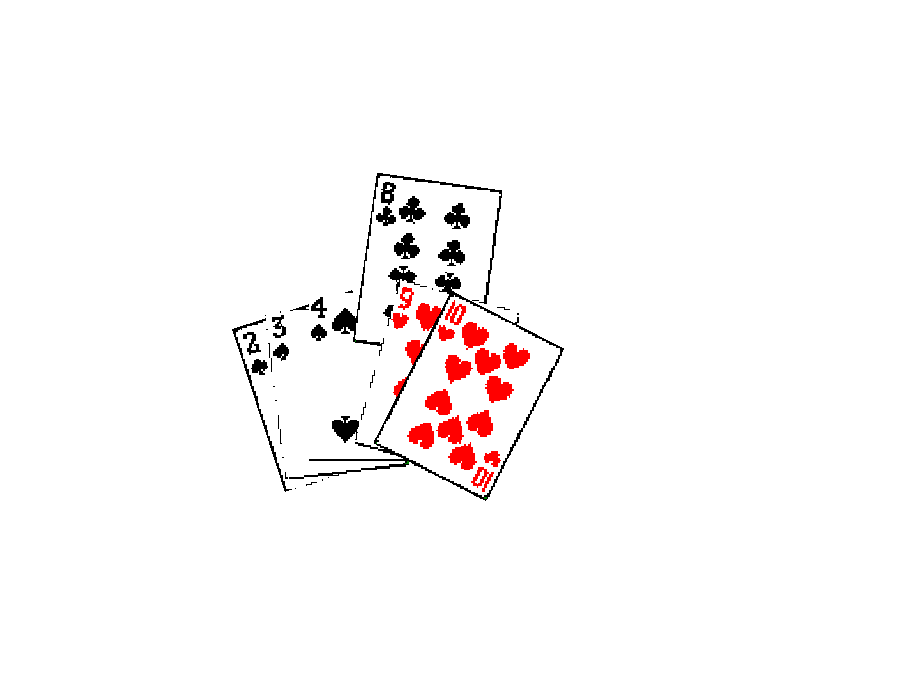
\includegraphics[scale=0.5]{img/hand-of-cards.eps}
  \caption{Insert card 8 to proper position in a deck.}
  \label{fig:hand-of-cards}
\end{figure}

Based on this idea, the algorithm of insertion sort can be directly
given as the following.

\begin{algorithmic}
\Function{Sort}{$A$}
  \State $X \gets \phi$
  \For{each $x \in A$}
    \State \Call{Insert}{$X, x$}
  \EndFor
  \State \Return $X$
\EndFunction
\end{algorithmic}

It's easy to express this process with folding, which we
mentioned in the chapter of binary search tree.

\be
  insert = foldL \quad insert \quad \phi
\ee

Note that in above algorithm, we store the sorted result in $X$,
so this isn't in-place sorting. It's easy to change it to in-place
algorithm. Denote the sequence as $A = \{a_1, a_2, ..., a_n\}$.

\begin{algorithmic}
\Function{Sort}{$A$}
  \For{$i \gets 2$ to $|A|$}
    \State insert $a_i$ to sorted sequence $\{a'_1, a'_2, ..., a'_{i-1} \}$
  \EndFor
\EndFunction
\end{algorithmic}

At any time, when we process the $i$-th element, all elements before $i$
have already been sorted. we continuously insert the current elements
until consume all the unsorted data. This idea is illustrated as in figure
\ref{fig:in-place-sort}.

\begin{figure}[htbp]
  \centering
  \includegraphics[scale=0.8]{img/in-place-sort.ps}
  \caption{The left part is sorted data, continuously insert elements to sorted part.}
  \label{fig:in-place-sort}
\end{figure}

We can find there is recursive concept in this definition. Thus it can
be expressed as the following.

\be
sort(A) = \left \{
  \begin{array}
  {r@{\quad:\quad}l}
  \phi & A = \phi \\
  insert(sort(\{a_2, a_3, ...\}), a_1) & otherwise
  \end{array}
\right.
\ee

% ================================================================
% Insertion
% ================================================================
\section{Insertion}
\index{insertion sort!insertion}

We haven't answered the question about how to realize insertion however.
It's a puzzle how does human locate the proper position so quickly.

For computer, it's an obvious option to perform a scan. We can either
scan from left to right or vice versa. However, if the sequence is
stored in plain array, it's necessary to scan from right to left.

\begin{algorithmic}
\Function{Sort}{$A$}
  \For{$i \gets 2$ to $|A|$}
    \Comment{Insert $A[i]$ to sorted sequence $A[1...i-1]$}
    \State $x \gets A[i]$
    \State $j \gets i-1$
    \While{$j > 0 \land x < A[j]$ }
      \State $A[j+1] \gets A[j]$
      \State $j \gets j - 1$
    \EndWhile
    \State $A[j+1] \gets x$
  \EndFor
\EndFunction
\end{algorithmic}

One may think scan from left to right is natural. However, it isn't
as effect as above algorithm for plain array. The reason is that, it's
expensive to insert an element in arbitrary position in an array.
As array stores elements continuously, if we want to insert new element
$x$ in position $i$, we must shift all elements after $i$, including
$i+1, i+2, ...$ one position to right. After that the cell at position $i$
is empty, and we can put $x$ in it. This is illustrated in
figure \ref{fig:array-shift}.

\begin{figure}[htbp]
  \centering
  \includegraphics[scale=0.7]{img/array-shift.ps}
  \caption{Insert $x$ to array $A$ at position $i$.}
  \label{fig:array-shift}
\end{figure}

If the length of array is $n$, this indicates we need examine the
first $i$ elements, then perform
$n-i+1$ moves, and then insert $x$ to the $i$-th cell. So insertion
from left to right need traverse the whole array anyway.
While if we scan from right to
left, we examine $i$ elements at most, and perform the same
amount of moves.

Translate the above algorithm to Python yields the following code.

\lstset{language=Python}
\begin{lstlisting}
def isort(xs):
    n = len(xs)
    for i in range(1, n):
        x = xs[i]
        j = i - 1
        while j >= 0 and x < xs[j]:
            xs[j+1] = xs[j]
            j = j - 1
        xs[j+1] = x
\end{lstlisting}

It can be found some other equivalent programs, for instance the following
ANSI C program. However this version isn't as effective as the pseudo code.

\lstset{language=C}
\begin{lstlisting}
void isort(Key* xs, int n){
  int i, j;
  for(i=1; i<n; ++i)
    for(j=i-1; j>=0 && xs[j+1] < xs[j]; --j)
      swap(xs, j, j+1);
}
\end{lstlisting}

This is because the swapping function, which can exchange two elements
typically uses a temporary variable like the following:

\begin{lstlisting}
void swap(Key* xs, int i, int j){
  Key temp = xs[i];
  xs[i] = xs[j];
  xs[j] = temp;
}
\end{lstlisting}

So the ANSI C program presented above takes $3m$ times assignment, where $m$
is the number of inner loops. While the pseudo code as well as the Python
program use shift operation instead of swapping. There are $m+2$ times
assignment.

We can also provide \textproc{Insert}() function explicitly, and call it
from the general insertion sort algorithm in previous section. We skip
the detailed realization here and left it as an exercise.

All the insertion algorithms are bound to $O(n)$, where $n$ is the length of
the sequence. No matter what difference among them, such as scan from left
or from right. Thus the over all performance for insertion sort is quadratic
as $O(n^2)$.

\begin{Exercise}

\begin{itemize}
\item Provide explicit insertion function, and call it with general
insertion sort algorithm. Please realize it in both procedural way and
functional way.
\end{itemize}

\end{Exercise}

% ================================================================
% Improvement 1
% ================================================================

\section{Improvement 1}
\index{Insertion sort!binary search}

Let's go back to the question, that why human being can find the proper
position for insertion so quickly. We have shown a solution based on scan.
Note the fact that at any time, all cards at hands have been well sorted,
another possible solution is to use binary search to find that location.

We'll explain the search algorithms in other dedicated chapter. Binary
search is just briefly introduced for illustration purpose here.

The algorithm will be changed to call a binary search procedure.

\begin{algorithmic}
\Function{Sort}{$A$}
  \For{$i \gets 2$ to $|A|$}
    \State $x \gets A[i]$
    \State $p \gets $ \Call{Binary-Search}{$A[1...i-1], x$}
    \For{$j \gets i$ down to $p$}
      \State $A[j] \gets A[j-1]$
    \EndFor
    \State $A[p] \gets x$
  \EndFor
\EndFunction
\end{algorithmic}

Instead of scan elements one by one, binary search utilize the information
that all elements in slice of array $\{A_1, ..., A_{i-1} \}$ are sorted.
Let's assume
the order is monotonic increase order. To find a position $j$ that satisfies
$A_{j-1} \leq x \leq A_{j}$. We can first examine the middle element, for
example, $A_{\lfloor i/2 \rfloor}$. If $x$ is less than it, we need next recursively
perform binary search in the first half of the sequence; otherwise, we
only need search in last half.

Every time, we halve the elements to be examined, this search process runs
$O(\lg n)$ time to locate the insertion position.

\begin{algorithmic}
\Function{Binary-Search}{$A, x$}
  \State $l \gets 1$
  \State $u \gets 1+|A|$
  \While{$l < u$}
    \State $m \gets \lfloor \frac{l+u}{2} \rfloor$
    \If{$A[m] = x$}
      \State \Return $m$ \Comment{Find a duplicated element}
    \ElsIf{$A[m] < x$}
      \State $l \gets m+1$
    \Else
      \State $u \gets m$
    \EndIf
  \EndWhile
  \State \Return $l$
\EndFunction
\end{algorithmic}

The improved insertion sort algorithm is still bound to $O(n^2)$,
compare to previous section, which we use $O(n^2)$ times comparison and
$O(n^2)$ moves, with binary search, we just use $O(n \lg n)$ times
comparison and $O(n^2)$ moves.

The Python program regarding to this algorithm is given below.

\lstset{language=Python}
\begin{lstlisting}
def isort(xs):
    n = len(xs)
    for i in range(1, n):
        x = xs[i]
        p = binary_search(xs[:i], x)
        for j in range(i, p, -1):
            xs[j] = xs[j-1]
        xs[p] = x

def binary_search(xs, x):
    l = 0
    u = len(xs)
    while l < u:
        m = (l+u)/2
        if xs[m] == x:
            return m
        elif xs[m] < x:
            l = m + 1
        else:
            u = m
    return l
\end{lstlisting}

\begin{Exercise}
Write the binary search in recursive manner. You needn't use purely functional
programming language.
\end{Exercise}

% ================================================================
% Improvement 2
% ================================================================

\section{Improvement 2}
\index{Insertion sort!linked-list setting}

Although we improve the search time to $O(n \lg n)$ in previous section, the
number of moves is still $O(n^2)$. The reason of why movement takes so long
time, is because the sequence is stored in plain array. The nature of array
is continuously layout data structure, so the insertion operation is expensive.
This hints us that we can use linked-list setting to represent the sequence.
It can improve the insertion operation from $O(n)$ to constant time $O(1)$.

\be
  insert(A, x) = \left \{
  \begin{array}
  {r@{\quad:\quad}l}
  \{ x \} & A = \phi \\
  \{ x \} \cup A & x < a_1 \\
  \{ a_1 \} \cup insert(\{ a_2, a_3, ... a_n\}, x)& otherwise
  \end{array}
\right.
\ee

Translating the algorithm to Haskell yields the below program.

\lstset{language=Haskell}
\begin{lstlisting}
insert [] x = [x]
insert (y:ys) x = if x < y then x:y:ys else y:insert ys x
\end{lstlisting}

And we can complete the two versions of insertion sort program based on
the first two equations in this chapter.

\begin{lstlisting}
isort [] = []
isort (x:xs) = insert (isort xs) x
\end{lstlisting}

Or we can represent the recursion with folding.

\begin{lstlisting}
isort = foldl insert []
\end{lstlisting}

Linked-list setting solution can also be described imperatively. Suppose
function \textproc{Key}($x$), returns the value of element stored in node
$x$, and \textproc{Next}($x$) accesses the next node in the linked-list.

\begin{algorithmic}
\Function{Insert}{$L, x$}
  \State $p \gets$ NIL
  \State $H \gets L$
  \While{$L \neq$ NIL $\land $ \Call{Key}{$L$} $<$ \Call{Key}{$x$}}
    \State $p \gets L$
    \State $L \gets $ \Call{Next}{$L$}
  \EndWhile
  \State \Call{Next}{$x$} $\gets L$
  \If{$p \neq$ NIL}
    \State $H \gets x$
  \Else
    \State \Call{Next}{$p$} $\gets x$
  \EndIf
  \State \Return $H$
\EndFunction
\end{algorithmic}

For example in ANSI C, the linked-list can be defined as the following.

\lstset{language=C}
\begin{lstlisting}
struct node{
  Key key;
  struct node* next;
};
\end{lstlisting}

Thus the insert function can be given as below.

\begin{lstlisting}
struct node* insert(struct node* lst, struct node* x){
  struct node *p, *head;
  p = NULL;
  for(head = lst; lst && x->key > lst->key; lst = lst->next)
    p = lst;
  x->next = lst;
  if(!p)
    return x;
  p->next = x;
  return head;
}
\end{lstlisting}

Instead of using explicit linked-list such as by pointer or reference
based structure. Linked-list can also be realized by another index array.
For any array element $A[i]$, $Next[i]$ stores the index of next element
follows $A[i]$. It means $A[Next[i]]$ is the next element after $A[i]$.

The insertion algorithm based on this solution is given like below.

\begin{algorithmic}
\Function{Insert}{$A, Next, i$}
  \State $j \gets \perp$
  \While{$Next[j] \neq$ NIL $\land A[Next[j]] < A[i]$}
    \State $j \gets Next[j]$
  \EndWhile
  \State $Next[i] \gets Next[j]$
  \State $Next[j] \gets i$
\EndFunction
\end{algorithmic}

Here $\perp$ means the head of the $Next$ table.
And the relative Python program for this algorithm is given as the following.

\lstset{language=Python}
\begin{lstlisting}
def isort(xs):
    n = len(xs)
    next = [-1]*(n+1)
    for i in range(n):
        insert(xs, next, i)
    return next

def insert(xs, next, i):
    j = -1
    while next[j] != -1 and xs[next[j]] < xs[i]:
        j = next[j]
    next[j], next[i] = i, next[j]
\end{lstlisting}

Although we change the insertion operation to constant time by using
linked-list. However, we have to traverse the linked-list to find the
position, which results $O(n^2)$ times comparison. This is because
linked-list, unlike array, doesn't support random access. It means we
can't use binary search with linked-list setting.

\begin{Exercise}
\begin{itemize}
\item Complete the insertion sort by using linked-list insertion function
in your favorate imperative programming language.
\item The index based linked-list return the sequence of rearranged index
as result. Write a program to re-order the original array of elements from
this result.
\end{itemize}
\end{Exercise}

% ================================================================
% Final improvement
% ================================================================

\section{Final improvement by binary search tree}
\index{Insertion sort!binary search tree}

It seems that we drive into a corner. We must improve both the comparison
and the insertion at the same time, or we will end up with $O(n^2)$ performance.

We must use binary search, this is the only way to improve the comparison
time to $O(\lg n)$. On the other hand, we must change the data structure,
because we can't achieve constant time insertion at a position with
plain array.

This remind us about our 'hello world' data structure, binary search tree.
It naturally support binary search from its definition. At the same time,
We can insert a new node in binary search tree in $O(1)$ constant time
if we already find the location.

So the algorithm changes to this.

\begin{algorithmic}
\Function{Sort}{$A$}
  \State $T \gets \phi$
  \For{each $x \in A$}
    \State $T \gets $ \Call{Insert-Tree}{$T, x$}
  \EndFor
  \State \Return \Call{To-List}{$T$}
\EndFunction
\end{algorithmic}

Where \textproc{Insert-Tree}() and \textproc{To-List}() are described in
previous chapter about binary search tree.

As we have analyzed for binary search tree, the performance of tree sort
is bound to $O(n \lg n)$, which is the lower limit of comparison based
sort\cite{Knuth}.

\section{Short summary}
In this chapter, we present the evolution process of insertion sort. Insertion
sort is well explained in most textbooks as the first sorting algorithm.
It has simple and straightforward idea, but the performance is quadratic.
Some textbooks stop here, but we want to show that there exist ways to improve
it by different point of view. We first try to save the comparison time
by using binary search, and then try to save the insertion operation by
changing the data structure to linked-list. Finally, we combine these
two ideas and evolute insertion sort to tree sort.

\begin{thebibliography}{99}

\bibitem{wiki-bubble-sort}
http://en.wikipedia.org/wiki/Bubble\_sort

\bibitem{CLRS}
Thomas H. Cormen, Charles E. Leiserson, Ronald L. Rivest and Clifford Stein.
``Introduction to Algorithms, Second Edition''. ISBN:0262032937. The MIT Press. 2001

\bibitem{Knuth}
Donald E. Knuth. ``The Art of Computer Programming, Volume 3: Sorting and Searching (2nd Edition)''. Addison-Wesley Professional; 2 edition (May 4, 1998) ISBN-10: 0201896850 ISBN-13: 978-0201896855

\end{thebibliography}

\ifx\wholebook\relax\else
\end{document}
\fi


\ifx\wholebook\relax \else

\documentclass[b5paper]{article}
\usepackage[nomarginpar
  %, margin=.5in
]{geometry}

\addtolength{\oddsidemargin}{-0.05in}
\addtolength{\evensidemargin}{-0.05in}
\addtolength{\textwidth}{0.1in}

\usepackage[en]{../../../prelude}

\setcounter{page}{1}

\begin{document}

\title{Red-black tree}

\author{Xinyu LIU
\thanks{{\bfseries Xinyu LIU} \newline
  Email: liuxinyu95@gmail.com \newline}
  }

\maketitle
\fi

\markboth{Red-black tree}{Elementary Algorithms}

\ifx\wholebook\relax
\chapter{Red-black tree}
\numberwithin{Exercise}{chapter}
\fi

As the example in chapter 2, we use the binary search tree as a dictionary to count the word occurrence. One may want to feed a address book to a binary search tree, and use it to lookup the contact as below example program:

\lstset{frame = single}
\begin{lstlisting}[language=Bourbaki]
void addrBook(Input in) {
    Map<String, String> dict
    while (String name, String addr) = read(in) {
        dict[name] = addr
    }
    loop {
        string name = read(Console)
        var addr = dict[name]
        if (addr == null) {
            print("not found")
        } else {
            print("address: ", addr)
        }
    }
}
\end{lstlisting}

Unlike the word counter program, this one performs poorly, especially when search names like Zara, Zed, Zulu, etc. This is because the address entries are typically in lexicographic order. If insert numbers 1, 2, 3, ..., $n$ to a binary search tree, it ends up like in figure \ref{fig:unbalanced-tree}. It is an extremely unbalanced binary search tree. The $lookup$ is bound to $O(h)$ time for a tree of height $h$. When the tree is well balanced, the performance is $O(\lg n)$, where $n$ is the number of elements. But in this extreme case, the performance downgrades to $O(n)$, same as list scan.

\begin{figure}[htbp]
  \centering
  \includegraphics[scale=0.5]{img/unbalanced}
  \caption{unbalanced tree}
  \label{fig:unbalanced-tree}
\end{figure}

\begin{Exercise}
\Question{For a big address entry list in lexicographic order, one may want to speed up building the address book with two concurrent tasks: one reads from the head; the other from the tail, till they meet at some middle point. What does the binary search tree look like? What if split the list into multiple sections to scale the concurrency?}
\Question{Find more cases to exploit a binary search tree, for example in figure \ref{fig:unbalanced-trees}.}
\end{Exercise}

\begin{figure}[htbp]
  \centering
  \includegraphics[scale=0.5]{img/unbalanced-trees}
  \caption{Unbalanced trees}
  \label{fig:unbalanced-trees}
\end{figure}

\section{Balance}
\index{tree rotation}

To avoid extremely unbalanced case, we can shuffle the input(\autoref{sec:bst-random-build} in chapter 2), however, when user enter input interactively, we can not randomize it. Most tree balancing solutions rely on the rotation operation. Rotation changes the tree structure while maintain the elements ordering. This chapter introduces the red-black tree, a popular self-balancing binary search tree. Next chapter is about AVL tree, another self-balanced tree. Chapter 8 introduces the splay tree. It adjusts the tree in steps. There are multiple binary search trees have the same in-order traverse result. Figure \ref{fig:tree-rotation} shows the tree rotation. We can define them with pattern matching:

\begin{figure}[htbp]
   \centering
   \includegraphics[scale=0.4]{img/tree-rotation}
   \caption{`left rotate' and `right rotate'.}
   \label{fig:tree-rotation}
\end{figure}

\be
\begin{array}{rcl}
rotate_l\ (a, x, (b, y, c)) & = & ((a, x, b), y, c)) \\
rotate_l\ T & = & T \\
\end{array}
\ee

and

\be
\begin{array}{rcl}
rotate_r\ ((a, x, b), y, c) & = & (a, x, (b, y, c)) \\
rotate_r\ T & = & T \\
\end{array}
\ee

Each second clause keeps the tree unchanged if the pattern does not match (for example, both sub-trees are empty). We can also implement tree rotation imperatively. We need re-assign sub-trees and parent reference. When rotate, we pass both the root $T$, and the node $x$ as parameters:

\begin{algorithmic}[1]
\Function{Left-Rotate}{$T, x$}
  \State $p \gets$ \Call{Parent}{$x$}
  \State $y \gets$ \Call{Right}{$x$} \Comment{assume $y \ne$ NIL}
  \State $a \gets$ \Call{Left}{$x$}
  \State $b \gets$ \Call{Left}{$y$}
  \State $c \gets$ \Call{Right}{$y$}
  \State \Call{Replace}{$x, y$}  \Comment{replace node $x$ with $y$}
  \State \Call{Set-Subtrees}{$x, a, b$} \Comment{Set $a, b$ as the sub-trees of $x$}
  \State \Call{Set-Subtrees}{$y, x, c$} \Comment{Set $x, c$ as the sub-trees of $y$}
  \If{$p = $ NIL}  \Comment{$x$ was the root}
    \State $T \gets y$
  \EndIf
  \State \Return $T$
\EndFunction
\end{algorithmic}

The \textproc{Right-Rotate} is symmetric, we leave it as exercise. The \textproc{Replace}($x$, $y$) uses node $y$ to replace $x$:

\begin{algorithmic}[1]
\Function{Replace}{$x, y$}
  \State $p \gets$ \Call{Parent}{$x$}
  \If{$p$ = NIL} \Comment{$x$ is the root}
    \If{$y \ne$ NIL}
           \Call{Parent}{$y$} $\gets$ NIL
    \EndIf
  \ElsIf{\Call{Left}{$p$} $= x$}
    \State \Call{Set-Left}{$p$, $y$}
  \Else
    \State \Call{Set-Right}{$p$, $y$}
  \EndIf
  \State \Call{Parent}{$x$} $\gets$ NIL
\EndFunction
\end{algorithmic}

Procedure \textproc{Set-Subtrees}($x, L, R$) assigns $L$ as the left, and $R$ as the right sub-trees of $x$:

\begin{algorithmic}[1]
\Function{Set-Subtrees}{$x, L, R$}
  \State \Call{Set-Left}{$x, L$}
  \State \Call{Set-Right}{$x, R$}
\EndFunction
\end{algorithmic}

It further calls \textproc{Set-Left} and \textproc{Set-Right} to set the two sub-trees:

\begin{algorithmic}[1]
\Function{Set-Left}{$x, y$}
  \State \Call{Left}{$x$} $\gets y$
  \If{$y \ne$ NIL}
    \Call{Parent}{$y$} $\gets x$
  \EndIf
  \EndFunction

\Statex

\Function{Set-Right}{$x, y$}
  \State \Call{Right}{$x$} $\gets y$
  \If{$y \ne$ NIL}
    \Call{Parent}{$y$} $\gets x$
  \EndIf
\EndFunction
\end{algorithmic}

We can see how pattern matching simplifies the tree rotation. Based on this idea, Okasaki developed the purely functional algorithm for red-black tree in 1995\cite{okasaki}.

\begin{Exercise}
\Question{Implement the \textproc{Right-Rotate}.}
\end{Exercise}

\section{Definition}
\index{red-black tree}

A red-black tree is a self-balancing binary search tree\cite{wiki-rbt}. It is equivalent to 2-3-4 tree\footnote{Chapter 7, B-tree. For any 2-3-4 tree, there is at least one red-black tree has the same ordered data.}. By coloring the node red or black, and performing rotation, red-black tree provides an efficient way to keep the tree balanced. On top of the binary search tree definition, we label the node with a color. We say it is a red-black tree if the coloring satisfies the following 5 rules(\cite{CLRS} pp273):

\index{red-black tree!red-black properties}
\begin{enumerate}
\item Every node is either red or black.
\item The root is black.
\item Every NIL node is black.
\item If a node is red, then both sub-trees are black.
\item For every node, all paths from it to descendant leaves contain the same number of black nodes.
\end{enumerate}

Why do they keep the red-black tree balanced? The key point is that, the longest path from the root to leaf can not exceed 2 times of the shortest path. Consider rule 4, there can not be any two adjacent red nodes. Hence the shortest path only contains black nodes. Any longer path must have red ones. In addition, rule 5 ensures all paths have the same number of black nodes. So as to the root. It eventually ensures any path can't exceed 2 times of the others\cite{wiki-rbt}. Figure \ref{fig:rbt-example-with-nil} gives an example of red-black tree.

\begin{figure}[htbp]
  \centering
  \includegraphics[scale=0.35]{img/rbt-example-with-nil}
  \caption{A red-black tree}
  \label{fig:rbt-example-with-nil}
\end{figure}

As all NIL nodes are black, we can hide them as shown in figure \ref{fig:rbt-example}. All operations including $lookup$, $\min/\max$, are same as the binary search tree. However, the $insert$ and $delete$ are special, as we need maintain the coloring rules. Below example program adds the color variable atop binary search tree definition. Denote the empty tree as $\nil$, the none empty tree as $(c, l, k,, r)$, where $c$ is the color (red/black), $k$ is the element, $l$ and $r$ are left and right sub-trees.

\begin{figure}[htbp]
  \centering
  \includegraphics[scale=0.4]{img/rbt-example}
  \caption{Hide the NIL nodes}
  \label{fig:rbt-example}
\end{figure}

\begin{Haskell}
data Color = R | B
data RBTree a = Empty | Node Color (RBTree a) a (RBTree a)
\end{Haskell}

\begin{Exercise}
\Question{Prove the height $h$ of a red-black tree of $n$ nodes is at most $2 \lg (n+1)$}
\end{Exercise}

\section{Insert}
\index{red-black tree!insert}

The $insert$ operation takes two steps. The first step is as same as the binary search tree. The second step if to resume the coloring if it becomes unbalanced. We always color the new element red unless it is the root. Hence don't break any coloring rules except the 4-th. Because it may bring two adjacent red nodes. There are 4 cases violate rule 4. They share the same structure after fixing\cite{okasaki} as shown in figure \ref{fig:insert-fix}.

\begin{figure}[htbp]
  \centering
  \includegraphics[scale=0.4]{img/insert-fix}
  \caption{Fix 4 cases to the same structure.}
  \label{fig:insert-fix}
\end{figure}

All 4 transformations move the redness one level up. When fix recursively bottom-up, it may color the root red, hence violate rule 2. We need revert the root black finally. With pattern matching, define a $balance$ function to fix the coloring. Denote the color as $\mathcal{C}$ with values black $\mathcal{B}$, and red $\mathcal{R}$.

\be
\begin{array}{rcl}
%\text{up left:} & & \\
balance\ \mathcal{B}\ (\mathcal{R}, (\mathcal{R}, a, x, b), y, c)\ z\ d & = & (\mathcal{R}, (\mathcal{B}, a, x, b), y, (\mathcal{B}, c, z, d)) \\
%\text{up right:} & & \\
balance\ \mathcal{B}, (\mathcal{R}, a, x, (\mathcal{R}, b, y, c))\ z\ d  & = & (\mathcal{R}, (\mathcal{B}, a, x, b), y, (\mathcal{B}, c, z, d)) \\
%\text{bottom left:} & & \\
balance\ \mathcal{B}\ a\ x\ (\mathcal{R}, b, y, (\mathcal{R}, c, z, d)) & = & (\mathcal{R}, (\mathcal{B}, a, x, b), y, (\mathcal{B}, c, z, d))  \\
%\text{bottom right:} & & \\
balance\ \mathcal{B}\ a\ x\ (\mathcal{R}, (\mathcal{R}, b, y, c), z, d) & = & (\mathcal{R}, (\mathcal{B}, a, x, b), y, (\mathcal{B}, c, z, d))  \\
%\text{otherwise:} & & \\
balance\ T & = & T \\
\end{array}
\ee

If none of the 4 patterns matches, we leave the tree unchanged. Define the red-black tree $insert$ as: $insert\ x\ T = makeBlack\ (ins\ x\ T)$, or in Curried form:

\be
insert x = makeBlack \circ ins\ x
\ee

Where:

\be
\begin{array}{rcl}
ins\ x\ \nil\ & = & (\mathcal{R}, \nil, x, \nil) \\
ins\ x\ (\mathcal{C}, l, k, r) & = & \begin{cases}
  x < k: & balance\ \mathcal{C}\ (ins\ x\ l)\ k\ r \\
  x > k: & balance\ \mathcal{C}\ l\ k\ (ins\ x\ r) \\
  \end{cases}
\end{array}
\ee

If the tree is empty, we create a red leaf of $x$; otherwise, compare $x$ and $k$, recursively insert $x$ to a sub-tree. After that, call $balance$ to fix the coloring, finally force the root to be black.

\be
makeBlack\ (\mathcal{C}, l, k, r) = (\mathcal{B}, l, k, r)
\ee

Below is the example program:

\begin{Haskell}
insert x = makeBlack . (ins x) where
    ins x Empty = Node R Empty x Empty
    ins x (Node color l k r)
        | x < k     = balance color (ins x l) k r
        | otherwise = balance color l k (ins x r)
    makeBlack (Node _ l k r) = Node B l k r

balance B (Node R (Node R a x b) y c) z d = Node R (Node B a x b) y (Node B c z d)
balance B (Node R a x (Node R b y c)) z d = Node R (Node B a x b) y (Node B c z d)
balance B a x (Node R b y (Node R c z d)) = Node R (Node B a x b) y (Node B c z d)
balance B a x (Node R (Node R b y c) z d) = Node R (Node B a x b) y (Node B c z d)
balance color l k r = Node color l k r
\end{Haskell}

We skip to handle the duplicated keys. If the key already exists, we can overwrite, drop, or store the values in a list (\cite{CLRS}, pp269). Figure \ref{fig:insert-example} shows two red-black trees built from sequence 11, 2, 14, 1, 7, 15, 5, 8, 4 and 1, 2, ..., 8. The second example is well balanced even for ordered input.

\begin{figure}[htbp]
  \centering
  \includegraphics[scale=0.35]{img/insert-haskell}
  \caption{Red-black tree examples}
  \label{fig:insert-example}
\end{figure}

The $insert$ performs top-down recursive fixing. It is bound to $O(h)$ time, where $h$ is the height. As the red-black tree coloring rules are maintained, $h$ is logarithm to $n$, the number of elements. The overall performance is $O(\lg n)$.

\begin{Exercise}
\Question{Implement the $insert$ without pattern matching, handle the 4 cases separately.}
\end{Exercise}

\section{Delete}
\index{red-black tree!delete}

Delete is more complex than insert. We can simplify the recursive implementation with pattern matching\footnote{Actually, we reuse the unchanged part to rebuild the tree in purely functional settings, known as the `persist' feature}. There are alternative implementation to mimic delete. Build a read-only tree for frequently looking up\cite{okasaki-blog}. When delete a node, mark it with a flag, and trigger tree rebuilding if such nodes exceeds 50\%. Delete may also violate the red-black tree coloring rules, hence need fixing. The violation only happens when delete a black node according to rule 5. The black nodes along the path decreases by one, causing not all paths contain the same number of black nodes. To resume the blackness, we introduce a special `doubly-black' node(\cite{CLRS}, pp290). Such a node is counted as 2 black nodes. When delete a black node $x$, move the blackness up to parent or down to a sub-tree. Let node $y$ accept the blackness. If $y$ was red, turn it black; if $y$ was already black, turn it `doubly-black' as $\mathcal{B}^2$. Below example program adds the `doubly-black' color.

\begin{Haskell}
data Color = R | B | BB
data RBTree a = Empty | BBEmpty | Node Color (RBTree a) a (RBTree a)
\end{Haskell}

Because ever NIL is black, when push the blackness down to NIL, it becomes `doubly-black' empty (\texttt{BBEmpty}, or bold $\pmb{\varnothing}$). The first step is normal binary search tree delete; then as the second step, if cut a black node off, shift the blackness, and fix the coloring.

\be
delete\ x = makeBlack \circ del\ x
\ee

This is Curried definition. When delete a singleton tree, it becomes empty. To cover this case, we modify $makeBlack$ as below:

\be
\begin{array}{rcl}
makeBlack\ \nil & = & \nil \\
makeBlack\ (\mathcal{C}, l, k, r) & = & (\mathcal{B}, l, k, r) \\
\end{array}
\ee

Where $del$ accepts $x$ and the tree:

\be
\resizebox{\linewidth}{!}{\ensuremath{
\begin{array}{rcl}
del\ x\ \nil\ & = & \nil \\
del\ x\ (\mathcal{C}, l, k, r) & = & \begin{cases}
  x < k: & fixB^2(\mathcal{C}, (del\ x\ l), k, r) \\
  x > k: & fixB^2(\mathcal{C}, l, k, (del\ x\ r)) \\
  x = k: & \begin{cases}
    l = \nil: & \text{if}\ \mathcal{C} = \mathcal{B}\ \text{then}\ shiftB\ r\ \text{else}\ r \\
    r = \nil: & \text{if}\ \mathcal{C} = \mathcal{B}\ \text{then}\ shiftB\ l\ \text{else}\ l \\
    \text{otherwise}: & fixB^2(\mathcal{C}, l, m, (del\ m\ r)), \text{where}: m = min(r) \\
  \end{cases}
\end{cases}
\end{array}
}}
\ee

When the tree is empty, the result is $\nil$; otherwise, we compare $x$ and $k$. If $x < k$, we recursively delete from left; otherwise delete from right. Because the recursive result may contain doubly-black node, we apply $fixB^2$ to fix. When $x = k$, we locate the node to cut. If either sub-tree is empty, we replace the node with the none empty sub-tree, then shift the blackness if the node is black. If neither sub-tree is empty, we cut the minimum $m = \min\ r$ off, and use $m$ to replace $k$. To reserve the blackness, $shiftB$ makes a black node doubly-black, and forces it black for other cases. It flips doubly-black to normal black when applied twice.

\be
\begin{array}{rcl}
shiftB\ (\mathcal{B}, l, k, r) & = & (\mathcal{B}^2, l, k, r) \\
shiftB\ (\mathcal{C}, l, k, r) & = & (\mathcal{B}, l, k, r) \\
shiftB\ \nil & = & \pmb{\nil} \\
shiftB\ \pmb{\nil} & = & \nil \\
\end{array}
\ee

Below is the example program (except the doubly-black fixing part).

\begin{Haskell}
delete x = makeBlack . (del x) where
    del x Empty = Empty
    del x (Node color l k r)
        | x < k = fixDB color (del x l) k r
        | x > k = fixDB color l k (del x r)
        | isEmpty l = if color == B then shiftBlack r else r
        | isEmpty r = if color == B then shiftBlack l else l
        | otherwise = fixDB color l m (del m r) where m = min r
    makeBlack (Node _ l k r) = Node B l k r
    makeBlack _ = Empty

isEmpty Empty = True
isEmpty _ = False

shiftBlack (Node B l k r) = Node BB l k r
shiftBlack (Node _ l k r) = Node B  l k r
shiftBlack Empty = BBEmpty
shiftBlack BBEmpty = Empty
\end{Haskell}

The $fixB^2$ function eliminates the doubly-black by rotation and re-coloring. The doubly-black node can be branch node or empty $\pmb{\varnothing}$. There are three cases:

\textbf{Case 1}. {\em The sibling of the doubly-black node is black, and it has a red sub-tree.} We can fix this case with a rotation. There are 4 sub-cases, all can transform to the same pattern, as shown in figure \ref{fig:del-case1}.

\begin{figure}[htbp]
  \centering
  \includegraphics[scale=0.4]{img/del-case1}
  \caption{Transform 4 sub-cases to the same pattern}
  \label{fig:del-case1}
\end{figure}

\be
\resizebox{\textwidth}{!}{\ensuremath{
\begin{array}{rcl}
%\text{case 1 up left:} & & \\
fixB^2\ \mathcal{C}\ a_{\mathcal{B}^2}\ x\ (\mathcal{B}, (\mathcal{R}, b, y, c), z, d) & = & (\mathcal{C}, (\mathcal{B}, shiftB(a), x, b), y, (\mathcal{B}, c, z, d)) \\
%\text{case 1 up right:} & & \\
fixB^2\ \mathcal{C}\ a_{\mathcal{B}^2}\ x\ (\mathcal{B}, b, y, (\mathcal{R}, c, z, d)) & = & (\mathcal{C}, (\mathcal{B}, shiftB(a), x, b), y, (\mathcal{B}, c, z, d)) \\
%\text{case 1 bottom left:} & & \\
fixB^2\ \mathcal{C}\ (\mathcal{B}, a, x, (\mathcal{R}, b, y, c))\ z\ d_{\mathcal{B}^2} & = & (\mathcal{C}, (\mathcal{B}, a, x, b), y, (\mathcal{B}, c, z, shiftB(d))) \\
%\text{case 1 bottom right:} & & \\
fixB^2\ \mathcal{C}\ (\mathcal{B}, (\mathcal{R}, a, x, b), y, c)\ z\ d_{\mathcal{B}^2} & = & (\mathcal{C}, (\mathcal{B}, a, x, b), y, (\mathcal{B}, c, z, shiftB(d))) \\
\end{array}
}}
\label{eq:db-case-1}
\ee

Where $a_{\mathcal{B}^2}$ means node $a$ is doubly-black.

\textbf{Case 2}. {\em The sibling of the doubly-black is red.} We can rotate the tree to turn it into case 1 or 3, as shown in figure \ref{fig:del-case2}. We add this fixing as additional 2 rows in equation (\ref{eq:db-case-1}):

\begin{figure}[htbp]
  \centering
  \includegraphics[scale=0.4]{img/del-case2}
  \caption{The sibling of the doubly-black is red.}
  \label{fig:del-case2}
\end{figure}

\be
%\resizebox{\textwidth}{!}{\ensuremath{
\begin{array}{rcl}
\text{...} & & \\
%\text{case 2 up:} & & \\
fixB^2\ \mathcal{B}\ a_{\mathcal{B}^2}\ x\ (\mathcal{R}, b, y, c) & = & fixB^2\ \mathcal{B}\ (fixB^2\ \mathcal{R}\ a\ x\ b)\ y\ c \\
%\text{case 2 bottom:} & & \\
fixB^2\ \mathcal{B}\ (\mathcal{R}, a, x, b)\ y\ c_{\mathcal{B}^2} & = & fixB^2\ \mathcal{B}\ a\ x\ (fixB^2\ \mathcal{R}\ b\ y\ c)
\end{array}
%}}
\label{eq:db-case-2}
\ee

\textbf{Case 3}. {\em The sibling of the doubly-black node, and its two sub-trees are all black.} In this case, we change the sibling to red, flip the doubly-black node to black, and propagate the doubly-blackness a level up to parent as shown in figure \ref{fig:del-case3}. There are two symmetric sub-cases. For the upper case, $x$ was either red or black. $x$ changes to black if it was red, otherwise changes to doubly-black; Same coloring changes to $y$ in the lower case. We add this fixing to equation (\ref{eq:db-case-2}):

\begin{figure}[htbp]
  \centering
  \includegraphics[scale=0.4]{img/del-case3}
  \caption{move the blackness up.}
  \label{fig:del-case3}
\end{figure}

\be
%\resizebox{\textwidth}{!}{\ensuremath{
\begin{array}{rcl}
\text{...} & & \\

fixB^2\ \mathcal{C}\ a_{\mathcal{B}^2}\ x\ (\mathcal{B}, b, y, c) & = & shiftB\ (\mathcal{C}, (shiftB\ a), x, (\mathcal{R}, b, y, c)) \\

fixB^2\ \mathcal{C}\ (\mathcal{B}, a, x, b)\ y\ c_{\mathcal{B}^2} & = & shiftB\ (\mathcal{C}, (\mathcal{R}, a, x, b), y, (shiftB\ c)) \\

fixB^2\ \mathcal{C}\ l\ k\ r\ & = & (\mathcal{C}, l, k, r) \\
\end{array}
%}}
\label{eq:db-case-3}
\ee

If none of the patterns match, the last row keeps the node unchanged. The doubly-black fixing is recursive. It terminates in two ways: One is \textbf{Case 1}, the doubly-black node is eliminated. Otherwise the blackness may move up till the root. Finally the we force the root be black. Below example program puts all three cases together:

\begin{Haskell}
fixDB color a@(Node BB _ _ _) x (Node B (Node R b y c) z d)
      = Node color (Node B (shiftBlack a) x b) y (Node B c z d)
fixDB color BBEmpty x (Node B (Node R b y c) z d)
      = Node color (Node B Empty x b) y (Node B c z d)
fixDB color a@(Node BB _ _ _) x (Node B b y (Node R c z d))
      = Node color (Node B (shiftBlack a) x b) y (Node B c z d)
fixDB color BBEmpty x (Node B b y (Node R c z d))
      = Node color (Node B Empty x b) y (Node B c z d)
fixDB color (Node B a x (Node R b y c)) z d@(Node BB _ _ _)
      = Node color (Node B a x b) y (Node B c z (shiftBlack d))
fixDB color (Node B a x (Node R b y c)) z BBEmpty
      = Node color (Node B a x b) y (Node B c z Empty)
fixDB color (Node B (Node R a x b) y c) z d@(Node BB _ _ _)
      = Node color (Node B a x b) y (Node B c z (shiftBlack d))
fixDB color (Node B (Node R a x b) y c) z BBEmpty
      = Node color (Node B a x b) y (Node B c z Empty)
fixDB B a@(Node BB _ _ _) x (Node R b y c)
      = fixDB B (fixDB R a x b) y c
fixDB B a@BBEmpty x (Node R b y c)
      = fixDB B (fixDB R a x b) y c
fixDB B (Node R a x b) y c@(Node BB _ _ _)
      = fixDB B a x (fixDB R b y c)
fixDB B (Node R a x b) y c@BBEmpty
      = fixDB B a x (fixDB R b y c)
fixDB color a@(Node BB _ _ _) x (Node B b y c)
      = shiftBlack (Node color (shiftBlack a) x (Node R b y c))
fixDB color BBEmpty x (Node B b y c)
      = shiftBlack (Node color Empty x (Node R b y c))
fixDB color (Node B a x b) y c@(Node BB _ _ _)
      = shiftBlack (Node color (Node R a x b) y (shiftBlack c))
fixDB color (Node B a x b) y BBEmpty
      = shiftBlack (Node color (Node R a x b) y Empty)
fixDB color l k r = Node color l k r
\end{Haskell}

The delete algorithm is bound to $O(h)$ time, where $h$ is the height of the tree. As red-black tree maintains the balance, $h = O(\lg n)$ for $n$ nodes.

\begin{Exercise}
\Question{Implement the `mark-rebuild' delete algorithm: mark the node as deleted without actually removing it. When the marked nodes exceed 50\%, rebuild the tree.}
\end{Exercise}

\section{Imperative red-black tree$\star$}
\index{red-black tree!imperative insertion}

We simplify the red-black tree implementation with pattern matching. In this section, we give the imperative algorithm for completeness. When insert, the first step is as same as the binary search tree, then as the second step, we fix the balance through tree rotations.

\begin{algorithmic}[1]
\Function{Insert}{$T, k$}
  \State $root \gets T$
  \State $x \gets$ \Call{Create-Leaf}{$k$}
  \State \Call{Color}{$x$} $\gets$ RED
  \State $p \gets$ NIL
  \While{$T \neq$ NIL}
    \State $p \gets T$
    \If{$k <$ \Call{Key}{$T$}}
      \State $T \gets $ \Call{Left}{$T$}
    \Else
      \State $T \gets $ \Call{Right}{$T$}
    \EndIf
  \EndWhile
  \State \Call{Parent}{$x$} $\gets p$
  \If{$p =$ NIL} \Comment{tree $T$ is empty}
    \State \Return $x$
  \ElsIf{$k <$ \Call{Key}{$p$}}
    \State \Call{Left}{$p$} $\gets x$
  \Else
    \State \Call{Right}{$p$} $\gets x$
  \EndIf
  \State \Return \Call{Insert-Fix}{$root, x$}
\EndFunction
\end{algorithmic}

We make the new node red, and then perform fixing before return. There are 3 basic cases, each one has a symmetric case, hence there are total 6 cases. Among them, we can merge two cases, because both have a red `uncle' node. We change the parent and uncle to black, and set grand parent to red:

\begin{algorithmic}[1]
\Function{Insert-Fix}{$T, x$}
  \While{\Call{Parent}{$x$} $\neq$ NIL and \textproc{Color}(\Call{Parent}{$x$}) = RED}
    \If{\textproc{Color}(\Call{Uncle}{$x$}) $=$ RED}
      \Comment{Case 1, $x$'s uncle is red}
      \State \textproc{Color}(\Call{Parent}{$x$}) $\gets$ BLACK
      \State \textproc{Color}(\Call{Grand-Parent}{$x$}) $\gets$ RED
      \State \textproc{Color}(\Call{Uncle}{$x$}) $\gets$ BLACK
      \State $x \gets$ \Call{Grand-Parent}{$x$}
    \Else
      \Comment{$x$'s uncle is black}
      \If{\Call{Parent}{$x$} = \textproc{Left}(\Call{Grand-Parent}{$x$})}
        \If{ $x =$ \textproc{Right}(\Call{Parent}{$x$})}
          \Comment{Case 2, $x$ is on the right}
          \State $x \gets$ \Call{Parent}{$x$}
          \State $T \gets$ \Call{Left-Rotate}{$T, x$}
        \EndIf
        \Comment{Case 3, $x$ is on the left}
        \State \textproc{Color}(\Call{Parent}{$x$}) $\gets$ BLACK
        \State \textproc{Color}(\Call{Grand-Parent}{$x$}) $\gets$ RED
        \State $T \gets$ \textproc{Right-Rotate}($T$, \Call{Grand-Parent}{$x$})
      \Else
        \If{ $x =$ \textproc{Left}(\Call{Parent}{$x$})}
          \Comment{Case 2, Symmetric}
          \State $x \gets$ \Call{Parent}{$x$}
          \State $T \gets$ \Call{Right-Rotate}{$T, x$}
        \EndIf
        \Comment{Case 3, Symmetric}
        \State \textproc{Color}(\Call{Parent}{$x$}) $\gets$ BLACK
        \State \textproc{Color}(\Call{Grand-Parent}{$x$}) $\gets$ RED
        \State $T \gets$ \textproc{Left-Rotate}($T$, \Call{Grand-Parent}{$x$})
      \EndIf
    \EndIf
  \EndWhile
  \State \Call{Color}{$T$} $\gets$ BLACK
  \State \Return $T$
\EndFunction
\end{algorithmic}

This algorithm takes $O(\lg n)$ time to insert a key, where $n$ is the number of nodes. Compare to the $balance$ function defined previously, they have different logic. Even input the same sequence of keys, they build different red-black trees. Figure \ref{fig:imperative-insert} shows the result when input the same sequence of keys to the imperative algorithm. We can see the difference from figure \ref{fig:insert-example}. There is a bit performance overhead in the pattern matching algorithm. Okasaki discussed the difference in detail in \cite{okasaki}.

\begin{figure}[htbp]
   \centering
   \includegraphics[scale=0.4]{img/clrs-fig-13-4}
   \includegraphics[scale=0.4]{img/python-insert}
   \caption{Red-black trees created by imperative algorithm.}
   \label{fig:imperative-insert}
\end{figure}

We provide the imperative delete algorithm in Appendix A of the book. Red-black tree is a popular self-balancing binary search tree. We introduce another one, AVL tree in the next chapter. Red-black tree is a good start for more complex data structures. If extend from 2 to $k$ sub-trees and maintain the balance, we obtain B-tree; If store the data along with the edge but not in node, we obtain the Radix tree. To maintain the balance, we need handle multiple cases. Okasaki's developed a method that makes the red-black tree easy to implement. There are many implementations based on this idea\cite{rosetta}. We also implement AVL tree and Splay tree based on pattern matching in this book.

\section{Appendix: Example programs}

Definition of red-black tree node with parent reference. Set the color red by default.

\begin{lstlisting}[language = Bourbaki]
data Node<T> {
    T key
    Color color
    Node<T> left
    Node<T> right
    Node<T> parent

    Node(T x) = Node(null, x, null, Color.RED)

    Node(Node<T> l, T k, Node<T> r, Color c) {
        left = l, key = k, right = r, color = c
        if left != null then left.parent = this
        if right != null then right.parent = this
    }

    Self setLeft(l) {
        left = l
        if l != null then l.parent = this
    }

    Self setRight(r) {
        right = r
        if r != null then r.parent = this
    }

    Node<T> sibling() = if parent.left == this then parent.right
                        else parent.left

    Node<T> uncle() = parent.sibling()

    Node<T> grandparent() = parent.parent
}
\end{lstlisting}

Insert a key to red-black tree:

\begin{lstlisting}[language = Bourbaki]
Node<T> insert(Node<T> t, T key) {
    root = t
    x = Node(key)
    parent = null
    while (t != null) {
        parent = t
        t = if (key < t.key) then t.left else t.right
    }
    if (parent == null) {    //tree is empty
        root = x
    } else if (key < parent.key) {
        parent.setLeft(x)
    } else {
        parent.setRight(x)
    }
    return insertFix(root, x)
}
\end{lstlisting}

Fix the balance:

\begin{lstlisting}[language = Bourbaki]
// Fix the red->red violation
Node<T> insertFix(Node<T> t, Node<T> x) {
    while (x.parent != null and x.parent.color == Color.RED) {
        if (x.uncle().color == Color.RED) {
            // case 1: ((a:R x:R b) y:B c:R) ==> ((a:R x:B b) y:R c:B)
            x.parent.color = Color.BLACK
            x.grandparent().color = Color.RED
            x.uncle().color = Color.BLACK
            x = x.grandparent()
        } else {
            if (x.parent == x.grandparent().left) {
                if (x == x.parent.right) {
                    // case 2: ((a x:R b:R) y:B c) ==> case 3
                    x = x.parent
                    t = leftRotate(t, x)
                }
                // case 3: ((a:R x:R b) y:B c) ==> (a:R x:B (b y:R c))
                x.parent.color = Color.BLACK
                x.grandparent().color = Color.RED
                t = rightRotate(t, x.grandparent())
            } else {
                if (x == x.parent.left) {
                    // case 2': (a x:B (b:R y:R c)) ==> case 3'
                    x = x.parent
                    t = rightRotate(t, x)
                }
                // case 3': (a x:B (b y:R c:R)) ==> ((a x:R b) y:B c:R)
                x.parent.color = Color.BLACK
                x.grandparent().color = Color.RED
                t = leftRotate(t, x.grandparent())
            }
        }
    }
    t.color = Color.BLACK
    return t
}
\end{lstlisting}

\ifx\wholebook\relax \else
\section{Answer}
\shipoutAnswer

\begin{thebibliography}{99}

\bibitem{CLRS}
Thomas H. Cormen, Charles E. Leiserson, Ronald L. Rivest and Clifford Stein.
``Introduction to Algorithms, Second Edition''. ISBN:0262032937. The MIT Press. 2001

\bibitem{okasaki}
Chris Okasaki. ``FUNCTIONAL PEARLS Red-Black Trees in a Functional Setting''. J. Functional Programming. 1998

\bibitem{okasaki-blog}
Chris Okasaki. ``Ten Years of Purely Functional Data Structures''. \url{http://okasaki.blogspot.com/2008/02/ten-years-of-purely-functional-data.html}

\bibitem{wiki-rbt}
Wikipedia. ``Red-black tree''. \url{https://en.wikipedia.org/wiki/Red-black_tree}

\bibitem{rosetta}
Pattern matching. \url{http://rosettacode.org/wiki/Pattern_matching}

\end{thebibliography}

\expandafter\enddocument
\fi


\ifx\wholebook\relax \else
% ------------------------

\documentclass{article}
%------------------- Other types of document example ------------------------
%
%\documentclass[twocolumn]{IEEEtran-new}
%\documentclass[12pt,twoside,draft]{IEEEtran}
%\documentstyle[9pt,twocolumn,technote,twoside]{IEEEtran}
%
%-----------------------------------------------------------------------------
%\input{../../../common.tex}
%
% loading packages
%

\RequirePackage{ifpdf}
\RequirePackage{ifxetex}

%
%
\ifpdf
  \RequirePackage[pdftex,%
       bookmarksnumbered,%
              colorlinks,%
          linkcolor=blue,%
              hyperindex,%
        plainpages=false,%
       pdfstartview=FitH]{hyperref}
\else\ifxetex
  \RequirePackage[bookmarksnumbered,%
               colorlinks,%
           linkcolor=blue,%
               hyperindex,%
         plainpages=false,%
        pdfstartview=FitH]{hyperref}
\else
  \RequirePackage[dvipdfm,%
        bookmarksnumbered,%
               colorlinks,%
           linkcolor=blue,%
               hyperindex,%
         plainpages=false,%
        pdfstartview=FitH]{hyperref}
\fi\fi
%\usepackage{hyperref}

% other packages
%--------------------------------------------------------------------------
\usepackage{graphicx, color}
\usepackage{subfig}
\usepackage{tikz}
\usetikzlibrary{matrix,positioning}

\usepackage{amsmath, amsthm, amssymb} % for math
\usepackage{exercise} % for exercise
\usepackage{import} % for nested input

%
% for programming
%
\usepackage{verbatim}
\usepackage{listings}
%\usepackage{algorithmic} %old version; we can use algorithmicx instead
\usepackage{algorithm}
\usepackage[noend]{algpseudocode} %for pseudo code, include algorithmicsx automatically
\usepackage{appendix}
\usepackage{makeidx} % for index support
\usepackage{titlesec}

\titleformat{\paragraph}
{\normalfont\normalsize\bfseries}{\theparagraph}{1em}{}
\titlespacing*{\paragraph}
{0pt}{3.25ex plus 1ex minus .2ex}{1.5ex plus .2ex}

\lstdefinelanguage{Smalltalk}{
  morekeywords={self,super,true,false,nil,thisContext}, % This is overkill
  morestring=[d]',
  morecomment=[s]{"}{"},
  alsoletter={\#:},
  escapechar={!},
  literate=
    {BANG}{!}1
    {UNDERSCORE}{\_}1
    {\\st}{Smalltalk}9 % convenience -- in case \st occurs in code
    % {'}{{\textquotesingle}}1 % replaced by upquote=true in \lstset
    {_}{{$\leftarrow$}}1
    {>>>}{{\sep}}1
    {^}{{$\uparrow$}}1
    {~}{{$\sim$}}1
    {-}{{\sf -\hspace{-0.13em}-}}1  % the goal is to make - the same width as +
    %{+}{\raisebox{0.08ex}{+}}1		% and to raise + off the baseline to match -
    {-->}{{\quad$\longrightarrow$\quad}}3
	, % Don't forget the comma at the end!
  tabsize=2
}[keywords,comments,strings]

% for better Haskell code outlook
\lstdefinelanguage{Haskell}{
  basicstyle=\small\ttfamily,
  flexiblecolumns=false,
  basewidth={0.5em,0.45em},
  literate={+}{{$+$}}1 {/}{{$/$}}1 {*}{{$*$}}1 {=}{{$=$}}1
           {>}{{$>$}}1 {<}{{$<$}}1 {\\}{{$\lambda$}}1
           {\\\\}{{\char`\\\char`\\}}1
           {->}{{$\rightarrow$}}2 {>=}{{$\geq$}}2 {<-}{{$\leftarrow$}}2
           {<=}{{$\leq$}}2 {=>}{{$\Rightarrow$}}2
           {\ .}{{$\circ$}}2 {\ .\ }{{$\circ$}}2
           {>>}{{>>}}2 {>>=}{{>>=}}2
           {|}{{$\mid$}}1
}[keywords,comments,strings]

\lstloadlanguages{C, C++, Lisp, Haskell, Python, Smalltalk}

\lstset{
  showstringspaces = false
}

% ======================================================================

\def\BibTeX{{\rm B\kern-.05em{\sc i\kern-.025em b}\kern-.08em
    T\kern-.1667em\lower.7ex\hbox{E}\kern-.125emX}}

%
% mathematics
%
\newcommand{\be}{\begin{equation}}
\newcommand{\ee}{\end{equation}}
\newcommand{\bmat}[1]{\left( \begin{array}{#1} }
\newcommand{\emat}{\end{array} \right) }
\newcommand{\VEC}[1]{\mbox{\boldmath $#1$}}

% numbered equation array
\newcommand{\bea}{\begin{eqnarray}}
\newcommand{\eea}{\end{eqnarray}}

% equation array not numbered
\newcommand{\bean}{\begin{eqnarray*}}
\newcommand{\eean}{\end{eqnarray*}}

\newtheorem{theorem}{Theorem}[section]
\newtheorem{lemma}[theorem]{Lemma}
\newtheorem{proposition}[theorem]{Proposition}
\newtheorem{corollary}[theorem]{Corollary}


\setcounter{page}{1}

\begin{document}

%--------------------------

% ================================================================
%                 COVER PAGE
% ================================================================

\title{AVL tree}

\author{Larry~LIU~Xinyu
\thanks{{\bfseries Larry LIU Xinyu } \newline
  Email: liuxinyu95@gmail.com \newline}
  }

\maketitle
\fi

\markboth{AVL tree}{Elementary Algorithms}

\ifx\wholebook\relax
\chapter{AVL tree}
\numberwithin{Exercise}{chapter}
\fi

% ================================================================
%                 Introduction
% ================================================================
\section{Introduction}
\label{introduction} \index{AVL tree}

\subsection{How to measure the balance of a tree?}
Besides red-black tree, are there any other intuitive solutions of self-balancing
binary search tree? In order to measure how balancing a binary search tree is,
one idea is to compare the height of the right sub-tree and left sub-tree.
If they differs a lot, the tree isn't well balanced. Let's denote the
difference height between two children as below

\be
  \delta(T) = |R| - |L|
\ee

Where $|T|$ means the height of tree $T$, and $L$, $R$ denotes the left
sub-tree and right sub-tree.

If $\delta(T) = 0$, The tree is definitely balanced. For example, a
complete binary tree has $n=2^h-1$ nodes for height $h$. There is
no empty branches unless the leafs. Another trivial case is empty
tree. $\delta(\phi) = 0$. The less absolute value of $\delta(T)$
the more balancing the tree is.

We define $\delta(T)$ as the {\em balance factor} of a binary search
tree.

% ================================================================
% Definition
% ================================================================
\section{Definition of AVL tree}
\index{AVL tree!definition}

An AVL tree is a special binary search tree, that all sub-trees
satisfying the following criteria.

\be
  |\delta(T)| \leq 1
\ee

The absolute value of balance factor is less than or equal to 1, which
means there are only three valid values, -1, 0 and 1. Figure \ref{fig:avl-example} shows an example AVL tree.

\begin{figure}[htbp]
   \centering
   \includegraphics[scale=0.5]{img/avl-example.ps}
   \caption{An example AVL tree} \label{fig:avl-example}
\end{figure}


Why AVL tree can keep the tree balanced? In other words, Can this definition
ensure the height of the tree as $O(\lg n)$ where $n$ is the number of
the nodes in the tree? Let's prove this fact.

For an AVL tree of height $h$, The number of nodes varies. It can have at
most $2^h-1$ nodes for a complete binary tree. We are interesting about
how many nodes there are at least. Let's denote the minimum number of nodes
for height $h$ AVL tree as $N(h)$. It's obvious for the trivial cases
as below.

\begin{itemize}
\item For empty tree, $h=0$, $N(0)=0$;
\item For a singleton root, $h=1$, $N(1)=1$;
\end{itemize}

What's the situation for common case $N(h)$? Figure \ref{fig:N-h-relation}
shows an AVL tree $T$ of height $h$. It contains three part, the root node,
and two sub trees $L, R$. We have the following fact.

\be
  h= max(|L|, |R|) + 1
\ee

We immediately know that, there must be one child has height $h-1$. According
to the definition of AVL tree, we have
$||L|-|B|| \leq 1$. This leads to the fact that the height of
other tree can't be lower than $h-2$, So the total number of the nodes
of $T$ is the number of nodes in both children plus 1 (for the root node).
We exclaim that.

\be
  N(h) = N(h-1) + N(h-2) + 1
  \label{eq:Fibonacci-like}
\ee

\begin{figure}[htbp]
   \centering
   \includegraphics[scale=0.5]{img/Nh-lvr.ps}
   \caption{An AVL tree with height $h$, one of the sub-tree with height $h-1$, the other is no less than $h-2$} \label{fig:N-h-relation}
\end{figure}

This recursion reminds us the famous Fibonacci series. Actually we can
transform it to Fibonacci series by defining $N'(h) = N(h)+1$. So equation
(\ref{eq:Fibonacci-like}) changes to.

\be
  N'(h) = N'(h-1) + N'(h-2)
\ee

\begin{lemma}
\label{lemma:N-phi}
Let $N(h)$ be the minimum number of nodes for an AVL tree with
height $h$. and $N'(h) = N(h) + 1$, then
\be
  N'(h) \geq \phi^h
\ee

Where $\phi = \frac{\sqrt{5}+1}{2}$ is the golden ratio.
\end{lemma}

\begin{proof}
For the trivial case, we have
\begin{itemize}
\item $h=0$, $N'(0) = 1 \geq \phi^0 = 1$
\item $h=1$, $N'(1) = 2 \geq \phi^1 = 1.618...$
\end{itemize}

For the induction case, suppose $N'(h) \geq \phi^h$.
\[
  \begin{array}{lll}
  N'(h+1) & = N'(h) + N'(h-1) & \{Fibonacci\} \\
          & \geq \phi^h + \phi^{h-1} & \\
          & = \phi^{h-1}(\phi + 1) & \{\phi + 1 = \phi^2 = \frac{\sqrt{5}+3}{2}\} \\
          & = \phi^{h+1}
 \end{array}
\]
\end{proof}

From Lemma \ref{lemma:N-phi}, we immediately get

\be
  h \leq log_{\phi}(n+1) = log_{\phi}2 \cdot \lg (n+1) \approx 1.44 \lg (n+1)
  \label{eq:AVL-height}
\ee

It tells that the height of AVL tree is proportion to $O(\lg n)$, which
means that AVL tree is balanced.

During the basic mutable tree operations such as insertion and deletion,
if the balance factor changes to any invalid value, some fixing has
to be performed to resume $|\delta|$ within 1. Most implementations utilize
tree rotations. In this chapter, we'll show the pattern matching solution
which is inspired by Okasaki's red-black tree solution\cite{okasaki}.
Because of this modify-fixing approach, AVL tree is also a kind of
self-balancing binary search tree. For comparison purpose, we'll also
show the procedural algorithms.

Of course we can compute the $\delta$ value recursively, another option
is to store the balance factor inside each nodes, and update them
when we modify the tree. The latter one avoid computing the same value
every time.

Based on this idea, we can add one data field $\delta$ to the original
binary search tree as the following C++ code example \footnote{Some implementations store the height of a tree instead of $\delta$ as in \cite{py-avl}}.

\lstset{language=C++}
\begin{lstlisting}
template <class T>
struct node{
  int delta;
  T key;
  node* left;
  node* right;
  node* parent;
};
\end{lstlisting}

In purely functional setting, some implementation use different
constructors to store the $\delta$ information. for example in
\cite{hackage}, there are 4 constructors, \texttt{E}, \texttt{N}, \texttt{P}, \texttt{Z} defined.
\texttt{E} for empty tree, \texttt{N} for tree with negative 1 balance factor,
\texttt{P} for tree with positive 1 balance factor and \texttt{Z} for zero case.

In this chapter, we'll explicitly store the balance factor inside
the node.

\lstset{language=Haskell}
\begin{lstlisting}
data AVLTree a = Empty
               | Br (AVLTree a) a (AVLTree a) Int
\end{lstlisting}

The immutable operations, including looking up, finding the maximum
and minimum elements are all same as the binary search tree. We'll
skip them and focus on the mutable operations.

% ================================================================
%                 Insertion
% ================================================================
\section{Insertion}
\index{AVL tree!insertion}

Insert a new element to an AVL tree may violate the AVL tree property
that the $\delta$ absolute value exceeds 1. To resume it, one option
is to do the tree rotation according to the different insertion cases.
Most implementation is based on this approach

Another way is to use the similar pattern matching method mentioned by
Okasaki in his red-black tree implementation \cite{okasaki}. Inspired
by this idea, it is possible to provide a simple and intuitive
solution.

When insert a new key to the AVL tree, the balance factor of the
root may {\em changes} in range $[-1, 1]$\footnote{Note that, it doesn't mean $\delta$ is in range $[-1, 1]$, the changes of $\delta$ is in this range.}, and the height may increase
at most by one, which we need recursively use this information
to update the $\delta$ value in further level nodes. We can define
the result of the insertion algorithm as a pair of data
$(T', \Delta H)$. Where $T'$ is the new tree and $\Delta H$ is the
increment of height. Let's denote function $first(pair)$
can return the first element in a pair. We can modify
the binary search tree insertion algorithm as the following to
handle AVL tree.

\be
insert(T, k) = first(ins(T, k))
\ee

where

\be
ins(T, k) = \left \{
  \begin{array}
  {r@{\quad:\quad}l}
  ((\phi, k, \phi, 0), 1) & T = \phi \\
  tree(ins(L, k), k', (R, 0), \Delta) & k < k' \\
  tree((L, 0), k', ins(R, k), \Delta) & otherwise
  \end{array}
\right.
\label{eq:ins}
\ee

$L, R, k', \Delta$ represent the left child, right child, the key and
the balance factor of a tree.

\[
  \begin{array}{l}
  L = left(T) \\
  R = right(T) \\
  k' = key(T) \\
  \Delta = \delta(T)
  \end{array}
\]

When we insert a new key $k$ to a AVL tree $T$, if the tree is
empty, we just need create a leaf node with $k$, set the balance
factor as 0, and the height is increased by one. This is the trivial
case.

If $T$ isn't empty, we need compare the key $k'$ with $k$.
If $k$ is less than the key, we recursively insert it to the left
child, otherwise we insert it into the right child.

As we defined above, the result of the recursive insertion is a
pair like $(L', \Delta H_l)$, we need do balancing adjustment as well
as updating the increment of height. Function $tree()$ is defined
to dealing with this task. It takes 4 parameters as $(L', \Delta H_l)$,
$k'$, $(R', \Delta H_r)$, and $\Delta$. The result of this function
is defined as $(T', \Delta H)$, where $T'$ is the new tree after
adjustment, and $\Delta H$ is the new increment of height which is
defined as

\be
  \Delta H = |T'| - |T|
\ee

This can be further detailed deduced in 4 cases.

\be
\begin{array}{rl}
  \Delta H & = |T'| - |T| \\
              & = 1 + max(|R'|, |L'|) - (1 + max(|R|, |L|)) \\
              & = max(|R'|, |L'|) - max(|R|, |L|) \\
              & = \left \{
                  \begin{array}{r@{\quad:\quad}l}
                  \Delta H_r & \Delta \geq 0 \land \Delta' \geq 0 \\
                  \Delta + \Delta H_r & \Delta \leq 0 \land \Delta' \geq 0 \\
                  \Delta H_l - \Delta & \Delta \geq 0 \land \Delta' \leq 0 \\
                  \Delta H_l & otherwise
                  \end{array} \right .
\end{array}
\ee

To prove this equation, note the fact that the height can't increase
both in left and right with only one insertion.

These 4 cases can be explained from the balance factor
definition that it equals to the difference from the right sub tree
and left sub tree.

\begin{itemize}
\item If $\Delta \geq 0$ and $\Delta' \geq 0$, it means that the height
of right sub tree isn't less than the height of left sub tree both
before insertion and after insertion. In this case, the increment in
height of the tree is only `contributed' from the right sub tree, which
is $\Delta H_r$.

\item If $\Delta \leq 0$, which means the height of left sub tree isn't
less than the height of right sub tree before, and it becomes
$\Delta' \geq 0$,
which means that the height of right sub tree increases due to insertion,
and the left side keeps same ($|L'|=|L|$). So the increment in height is
\[
\begin{array}{rll}
\Delta H & = max(|R'|, |L'|) - max (|R|, |L|) & \{\Delta \leq 0 \land \Delta' \geq 0 \}\\
         & = |R'|-|L| & \{|L|=|L'| \}\\
         & = |R|+\Delta H_r - |L| & \\
         & = \Delta + \Delta H_r &
\end{array}
\]

\item For the case $\Delta \geq 0$ and $\Delta' \leq 0$, Similar as the
second one, we can get.

\[
\begin{array}{rll}
\Delta H & = max(|R'|, |L'|) - max (|R|, |L|) & \{\Delta \geq 0 \land \Delta' \leq 0 \}\\
         & = |L'|-|R| & \\
         & = |L|+\Delta H_l - |R| & \\
         & = \Delta H_l - \Delta&
\end{array}
\]

\item For the last case, the both $\Delta$ and $\Delta'$ is no bigger than
zero, which means the height left sub tree is always greater than or equal
 to the right sub tree, so the increment in height is only `contributed'
from the left sub tree, which is $\Delta H_l$.
\end{itemize}

The next problem in front of us is how to determine the new balancing
factor value $\Delta'$ before performing balancing adjustment.
According to the definition of AVL tree, the balancing factor is the
height of right sub tree minus the height of left sub tree. We have
the following facts.

\be
\begin{array}{rl}
\Delta' & = |R'| - |L'| \\
        & = |R| + \Delta H_r - (|L| + \Delta H_l) \\
        & = |R| - |L| + \Delta H_r - \Delta H_l \\
        & = \Delta + \Delta H_r - \Delta H_l
\end{array}
\ee

With all these changes in height and balancing factor get clear, it's
possible to define the $tree()$ function mentioned in (\ref{eq:ins}).

\be
tree((L', \Delta H_l), Key, (R', \Delta H_r), \Delta) =
  balance (node(L', Key, R', \Delta'), \Delta H)
\ee

Before we moving into details of balancing adjustment, let's translate
the above equations to real programs in Haskell.

First is the insert function.

\lstset{language=Haskell}
\begin{lstlisting}
insert::(Ord a)=>AVLTree a -> a -> AVLTree a
insert t x = fst $ ins t where
    ins Empty = (Br Empty x Empty 0, 1)
    ins (Br l k r d)
        | x < k     = tree (ins l) k (r, 0) d
        | x == k    = (Br l k r d, 0)
        | otherwise = tree (l, 0) k (ins r) d
\end{lstlisting} %$

Here we also handle the case that inserting a duplicated key (which
means the key has already existed.) as just overwriting.

\begin{lstlisting}
tree::(AVLTree a, Int) -> a -> (AVLTree a, Int) -> Int -> (AVLTree a, Int)
tree (l, dl) k (r, dr) d = balance (Br l k r d', delta) where
    d' = d + dr - dl
    delta = deltaH d d' dl dr
\end{lstlisting}

And the definition of height increment is as below.

\begin{lstlisting}
deltaH :: Int -> Int -> Int -> Int -> Int
deltaH d d' dl dr
       | d >=0 && d' >=0 = dr
       | d <=0 && d' >=0 = d+dr
       | d >=0 && d' <=0 = dl - d
       | otherwise = dl
\end{lstlisting}

\subsection{Balancing adjustment}
\index{AVL tree!balancing}
As the pattern matching approach is adopted in doing re-balancing.
We need consider what kind of patterns violate the AVL tree property.

Figure \ref{fig:insert-fix} shows the 4 cases which need fix. For all
these 4 cases the balancing factors are either -2, or +2 which exceed
the range of $[-1, 1]$. After balancing adjustment, this factor turns
to be 0, which means the height of left sub tree is equal to the right
sub tree.

\begin{figure}[htbp]
   \begin{center}
     \setlength{\unitlength}{1cm}
     \begin{picture}(15, 15)
        % arrows
        \put(4.5, 9.5){\vector(1, -1){1}}
        \put(4.5, 5){\vector(1, 1){1}}
        \put(10, 9.5){\vector(-1, -1){1}}
        \put(10, 5){\vector(-1, 1){1}}
        % delta values
        \put(5, 13){$\delta(z) = -2$}
        \put(2.5, 12){$\delta(y) = -1$}
        \put(10, 13){$\delta(x) = 2$}
        \put(11.5, 11.5){$\delta(y) = 1$}
        \put(1.5, 5.5){$\delta(z) = -2$}
        \put(3.5, 4){$\delta(x) = 1$}
        \put(12, 5.5){$\delta(x) = 2$}
        \put(10.5, 4){$\delta(z) = -1$}
        \put(7.5, 10){$\delta'(y) = 0$}
        % graphics
	\put(0, 7){\includegraphics[scale=0.5]{img/insert-ll.ps}}
        \put(0, 0){\includegraphics[scale=0.5]{img/insert-lr.ps}}
        \put(7, 7){\includegraphics[scale=0.5]{img/insert-rr.ps}}
        \put(8.5, 0){\includegraphics[scale=0.5]{img/insert-rl.ps}}
        \put(2, 5){\includegraphics[scale=0.5]{img/insert-fixed.ps}}
      \end{picture}
     \caption{4 cases for balancing a AVL tree after insertion} \label{fig:insert-fix}
  \end{center}
\end{figure}

We call these four cases left-left lean, right-right lean, right-left lean,
and left-right lean cases in clock-wise direction from top-left. We denote
the balancing factor before fixing as $\delta(x), \delta(y)$, and $\delta(z)$, while after fixing, they changes to $\delta'(x), \delta'(y)$, and
$\delta'(z)$ respectively.

We'll next prove that, after fixing, we have $\delta(y)=0$ for all
four cases, and we'll provide the result values of $\delta'(x)$ and
$\delta'(z)$.

\subsubsection*{Left-left lean case}

As the structure of sub tree $x$ doesn't change due to fixing, we immediately get
$\delta'(x) = \delta(x)$.

Since $\delta(y) = -1$ and $\delta(z) = -2$, we have

\be
  \begin{array}{l}
  \delta(y) = |C| - |x| = -1 \Rightarrow |C| = |x| - 1 \\
  \delta(z) = |D| - |y| = -2 \Rightarrow |D| = |y| - 2
  \end{array}
  \label{eq:ll-cd}
\ee

After fixing.

\be
  \begin{array}{rll}
  \delta'(z) & = |D| - |C| & \{ From (\ref{eq:ll-cd}) \}\\
             & = |y| - 2 - (|x| - 1) & \\
             & = |y| - |x| - 1 & \{  x \text{ is child of } y \Rightarrow |y|-|x| = 1\} \\
             & = 0 &
  \end{array}
  \label{eq:ll-delta-z}
\ee

For $\delta'(y)$, we have the following fact after fixing.

\be
  \begin{array}{rll}
  \delta'(y) & = |z| - |x| & \\
             & = 1 + max(|C|, |D|) - |x| & \{ \text{By (\ref{eq:ll-delta-z}), we have} |C| = |D|\} \\
             & = 1 + |C| - |x| & \{ \text{By (\ref{eq:ll-cd})}\} \\
             & = 1 + |x| - 1 - |x| & \\
             & = 0 &
  \end{array}
\ee

Summarize the above results, the left-left lean case adjust the balancing
factors as the following.

\be
  \begin{array}{l}
  \delta'(x) = \delta(x) \\
  \delta'(y) = 0 \\
  \delta'(z) = 0
  \end{array}
\ee

\subsubsection*{Right-right lean case}

Since right-right case is symmetric to left-left case, we can easily achieve the result balancing factors as

\be
  \begin{array}{l}
  \delta'(x) = 0 \\
  \delta'(y) = 0 \\
  \delta'(z) = \delta(z)
  \end{array}
  \label{eq:rr-result}
\ee

\subsubsection*{Right-left lean case}

First let's consider $\delta'(x)$. After balance fixing, we have.

\be
  \delta'(x) = |B| - |A|
  \label{eq:rl-dx}
\ee

Before fixing, if we calculate the height of $z$, we can get.

\be
  \begin{array}{rll}
  |z| & = 1 + max(|y|, |D|) &  \{ \delta(z) = -1 \Rightarrow |y| > |D|\} \\
      & = 1 + |y| & \\
      & = 2 + max(|B|, |C|)
  \end{array}
  \label{eq:rl-z}
\ee

While since $\delta(x) = 2$, we can deduce that.

\be
  \begin{array}{rll}
  \delta(x) = 2 & \Rightarrow |z| - |A| = 2 & \{ \text{By (\ref{eq:rl-z})} \}\\
                & \Rightarrow 2 + max(|B|, |C|) - |A| = 2 & \\
                & \Rightarrow max(|B|, |C|) - |A| = 0 &
  \end{array}
  \label{eq:rl-ca}
\ee

If $\delta(y) = 1$, which means $|C| - |B| = 1$, it means

\be
  max(|B|, |C|)= |C| = |B|+1
\ee

Take this into (\ref{eq:rl-ca}) yields

\be
  \begin{array}{ll}
  |B|+1-|A| = 0 \Rightarrow |B|-|A|= -1 & \{ \text{By (\ref{eq:rl-dx}) } \} \\
  \Rightarrow \delta'(x) = -1 &
  \end{array}
\ee

If $\delta(y) \neq 1$, it means $max(|B|, |C|) = |B|$, taking this into
(\ref{eq:rl-ca}), yields.

\be
  \begin{array}{ll}
  |B| - |A| = 0  & \{ \text{By (\ref{eq:rl-dx})} \} \\
  \Rightarrow \delta'(x) = 0 &
  \end{array}
\ee

Summarize these 2 cases, we get relationship of $\delta'(x)$ and
$\delta(y)$ as the following.

\be
\delta'(x) = \left \{
  \begin{array}
  {r@{\quad:\quad}l}
  -1 & \delta(y) = 1 \\
  0 & otherwise
  \end{array}
\right.
\label{eq:rl-dx-dy}
\ee

For $\delta'(z)$ according to definition, it is equal to.

\be
  \begin{array}{rll}
    \delta'(z) & = |D| - |C| & \{ \delta(z) = -1 = |D| - |y| \} \\
               & = |y| - |C| - 1 & \{ |y| = 1 + max(|B|, |C|) \} \\
               & = max(|B|, |C|) - |C|
  \end{array}
  \label{eq:rl-dz}
\ee

If $\delta(y) = -1$, then we have $|C| - |B| = -1$, so $max(|B|, |C|) = |B| = |C| + 1$. Takes this into (\ref{eq:rl-dz}), we get $\delta'(z) = 1$.

If $\delta(y) \neq -1$, then $max(|B|, |C|) = |C|$, we get $\delta'(z)=0$.

Combined these two cases, the relationship between $\delta'(z)$ and $\delta(y)$ is as below.

\be
\delta'(z) = \left \{
  \begin{array}
  {r@{\quad:\quad}l}
  1 & \delta(y) = -1 \\
  0 & otherwise
  \end{array}
  \right.
  \label{eq:rl-dz-dy}
\ee

Finally, for $\delta'(y)$, we deduce it like below.

\be
  \begin{array}{rl}
  \delta'(y) & = |z| - |x| \\
             & = max(|C|, |D|) - max(|A|, |B|)
  \end{array}
  \label{eq:rl-dy}
\ee

There are three cases.
\begin{itemize}

\item If $\delta(y)=0$, it means $|B|=|C|$, and according to (\ref{eq:rl-dx-dy}) and (\ref{eq:rl-dz-dy}), we have $\delta'(x)=0 \Rightarrow |A| = |B|$, and $\delta'(z)=0 \Rightarrow |C|=|D|$, these lead to $\delta'(y)=0$.

\item If $\delta(y)=1$, From (\ref{eq:rl-dz-dy}), we have $\delta'(z)=0 \Rightarrow |C| = |D|$.
\[
  \begin{array}{rll}
  \delta'(y) & = max(|C|, |D|) - max(|A|, |B|) & \{|C|=|D|\} \\
             & = |C| - max(|A|, |B|) & \{\text{From (\ref{eq:rl-dx-dy}): $\delta'(x)=-1 \Rightarrow |B|-|A|=-1$} \} \\
             & = |C| - (|B| + 1) & \{ \delta(y) = 1 \Rightarrow |C|-|B|=1\} \\
             & = 0
  \end{array}
\]

\item If $\delta(y)=-1$, From (\ref{eq:rl-dx-dy}), we have $\delta'(x)=0 \Rightarrow |A|=|B|$.
\[
  \begin{array}{rll}
  \delta'(y) & = max(|C|, |D|) - max(|A|, |B|) & \{|A|=|B|\} \\
             & = max(|C|, |D|) - |B| & \{ \text{From (\ref{eq:rl-dz-dy}): $|D|-|C|=1$} \} \\
             & = |C| + 1 - |B| & \{  \delta(y) = -1 \Rightarrow |C|-|B|=-1\} \\
             & = 0
  \end{array}
\]

\end{itemize}

All three cases lead to the same result that $\delta'(y)=0$.

Collect all the above results, we get the new balancing factors after fixing as the following.

\be
  \begin{array}{l}
  \delta'(x) = \left \{
    \begin{array}
    {r@{\quad:\quad}l}
    -1 & \delta(y) = 1 \\
    0 & otherwise
    \end{array}
    \right. \\
  \delta'(y) = 0 \\
  \delta'(z) = \left \{
    \begin{array}
    {r@{\quad:\quad}l}
    1 & \delta(y) = -1 \\
    0 & otherwise
    \end{array}
    \right.
  \end{array}
  \label{eq:rl-result}
\ee

\subsubsection*{Left-right lean case}

Left-right lean case is symmetric to the Right-left lean case. By using
the similar deduction, we can find the new balancing factors are identical
to the result in (\ref{eq:rl-result}).

\subsection{Pattern Matching}
All the problems have been solved and it's time to define the final
pattern matching fixing function.

\be
balance(T, \Delta H) = \left \{
  \begin{array}
  {r@{\quad:\quad}l}
  (((A, x, B, \delta(x)), y, (C, z, D, 0), 0), 0) & P_{ll}(T) \\
  (((A, x, B, 0), y, (C, z, D, \delta(z)), 0), 0) & P_{rr}(T) \\
  (((A, x, B, \delta'(x)), y, (C, z, D, \delta'(z)), 0), 0) & P_{rl}(T) \lor P_{lr}(T) \\
  (T, \Delta H) & otherwise
  \end{array}
\right.
\ee

Where $P_{ll}(T)$ means the pattern of tree $T$ is left-left lean respectively. $\delta'(x)$ and $delta'(z)$ are defined in (\ref{eq:rl-result}). The four patterns are tested as below.

\be
\begin{array}{l}
P_{ll}(T): T = (((A, x, B, \delta(x)), y, C, -1), z, D, -2) \\
P_{rr}(T): T = (A, x, (B, y, node(C, z, D, \delta(z)), 1), 2) \\
P_{rl}(T): T = ((A, x, (B, y, C, \delta(y)), 1), z, D, -2) \\
P_{lr}(T): T = (A, x, ((B, y, C, \delta(y)), z, D, -1), 2)
\end{array}
\ee

Translating the above function definition to Haskell yields a simple
and intuitive program.

\begin{lstlisting}
balance (Br (Br (Br a x b dx) y c (-1)) z d (-2), _) =
        (Br (Br a x b dx) y (Br c z d 0) 0, 0)
balance (Br a x (Br b y (Br c z d dz)    1)    2, _) =
        (Br (Br a x b 0) y (Br c z d dz) 0, 0)
balance (Br (Br a x (Br b y c dy)    1) z d (-2), _) =
        (Br (Br a x b dx') y (Br c z d dz') 0, 0) where
    dx' = if dy ==  1 then -1 else 0
    dz' = if dy == -1 then  1 else 0
balance (Br a x (Br (Br b y c dy) z d (-1))    2, _) =
        (Br (Br a x b dx') y (Br c z d dz') 0, 0) where
    dx' = if dy ==  1 then -1 else 0
    dz' = if dy == -1 then  1 else 0
balance (t, d) = (t, d)
\end{lstlisting}

The insertion algorithm takes time proportion to the height of the
tree, and according to the result we proved above, its performance
is $O(\lg n)$ where $n$ is the number of elements stored in the AVL
tree.

\subsubsection{Verification}
\index{AVL tree!verification}
One can easily create a function to verify a tree is AVL tree.
Actually we need verify two things, first, it's a binary search tree;
second, it satisfies AVL tree property.

We left the first verification problem as an exercise to the reader.

In order to test if a binary tree satisfies AVL tree property, we can
test the difference in height between its two children, and recursively
test that both children conform to AVL property until we arrive at
an empty leaf.

\be
  avl?(T) = \left \{
  \begin{array}
  {r@{\quad:\quad}l}
  True & T = \phi \\
  avl?(L) \land avl?(R) \land ||R|-|L|| \leq 1 & otherwise
  \end{array}
  \right .
\ee

And the height of a AVL tree can also be calculate from the definition.

\be
  |T| = \left \{
  \begin{array}
  {r@{\quad:\quad}l}
  0 & T = \phi \\
  1 + max(|R|, |L|) & otherwise
  \end{array}
  \right .
\ee

The corresponding Haskell program is given as the following.

\begin{lstlisting}
isAVL :: (AVLTree a) -> Bool
isAVL Empty = True
isAVL (Br l _ r d) = and [isAVL l, isAVL r, abs (height r - height l) <= 1]

height :: (AVLTree a) -> Int
height Empty = 0
height (Br l _ r _) = 1 + max (height l) (height r)
\end{lstlisting}

\begin{Exercise}
Write a program to verify a binary tree is a binary search tree in your
favorite programming language. If you choose to use an imperative language,
please consider realize this program without recursion.
\end{Exercise}



% ================================================================
%                 Deletion
% ================================================================

\section{Deletion}
\index{AVL tree!deletion}

As we mentioned before, deletion doesn't make significant sense in
purely functional settings. As the tree is read only, it's typically
performs frequently looking up after build.

Even if we implement deletion, it's actually re-building the tree
as we presented in chapter of red-black tree. We left the deletion
of AVL tree as an exercise to the reader.

\begin{Exercise}

\begin{itemize}

\item Take red-black tree deletion algorithm as an example, write the
AVL tree deletion program in purely functional approach in your
favorite programming language.
\end{itemize}

\end{Exercise}

\section{Imperative AVL tree algorithm $\star$}
\index{AVL tree!imperative insertion}

We almost finished all the content in this chapter about AVL tree.
However, it necessary to show the traditional insert-and-rotate
approach as the comparator to pattern matching algorithm.

Similar as the imperative red-black tree algorithm, the strategy
is first to do the insertion as same as for binary search tree,
then fix the balance problem by rotation and return the final result.

\begin{algorithmic}[1]
\Function{Insert}{$T, k$}
  \State $root \gets T$
  \State $x \gets$ \Call{Create-Leaf}{$k$}
  \State \Call{$\delta$}{$x$} $\gets 0$
  \State $parent \gets$ NIL
  \While{$T \neq$ NIL}
    \State $parent \gets T$
    \If{$k <$ \Call{Key}{$T$}}
      \State $T \gets $ \Call{Left}{$T$}
    \Else
      \State $T \gets $ \Call{Right}{$T$}
    \EndIf
  \EndWhile
  \State \Call{Parent}{$x$} $\gets parent$
  \If{$parent =$ NIL} \Comment{tree $T$ is empty}
    \State \Return $x$
  \ElsIf{$k <$ \Call{Key}{$parent$}}
    \State \Call{Left}{$parent$} $\gets x$
  \Else
    \State \Call{Right}{$parent$} $\gets x$
  \EndIf
  \State \Return \Call{AVL-Insert-Fix}{$root, x$}
\EndFunction
\end{algorithmic}

Note that after insertion, the height of the tree may increase, so that
the balancing factor $\delta$ may also change, insert on right side will
increase $\delta$ by 1, while insert on left side will decrease it. By
the end of this algorithm, we need perform bottom-up fixing from node $x$
towards root.

We can translate the pseudo code to real programming language, such as
Python \footnote{C and C++ source code are available along with this book}.
\lstset{language=Python}
\begin{lstlisting}
def avl_insert(t, key):
    root = t
    x = Node(key)
    parent = None
    while(t):
        parent = t
        if(key < t.key):
            t = t.left
        else:
            t = t.right
    if parent is None: #tree is empty
        root = x
    elif key < parent.key:
        parent.set_left(x)
    else:
        parent.set_right(x)
    return avl_insert_fix(root, x)
\end{lstlisting}

This is a top-down algorithm. It searches the tree from root down to the proper
position and inserts the new key as a leaf. By the end of this algorithm, it calls fixing procedure, by passing the root and the new node inserted.

Note that we reuse the same methods of \texttt{set\_left()} and \texttt{set\_right()} as
we defined in chapter of red-black tree.

In order to resume the AVL tree balance property by fixing, we first determine if the new node is inserted on left hand or right hand. If it is on left, the balancing factor $\delta$ decreases, otherwise it increases. If we denote the new value as $\delta'$, there are 3 cases of the relationship between $\delta$ and $\delta'$.

\begin{itemize}
\item If $|\delta| = 1$ and $|\delta'| = 0$, this means adding the new node makes the tree perfectly balanced, the height of the parent node doesn't change, the algorithm can be terminated.

\item If $|\delta| = 0$ and $|\delta'| = 1$, it means that either the height of left sub tree or right sub tree increases, we need go on check the upper level of the tree.

\item If $|\delta| = 1$ and $|\delta'| = 2$, it means the AVL tree property is violated due to the new insertion. We need perform rotation to fix it.
\end{itemize}

\begin{algorithmic}[1]
\Function{AVL-Insert-Fix}{$T, x$}
  \While{\Call{Parent}{$x$} $\neq$ NIL}
    \State $\delta \gets $ \textproc{$\delta$}(\Call{Parent}{$x$})
    \If{$x = $ \textproc{Left}(\Call{Parent}{$x$})}
      \State $\delta' \gets \delta - 1$
    \Else
      \State $\delta' \gets \delta + 1$
    \EndIf
    \State \textproc{$\delta$}(\Call{Parent}{$x$}) $\gets \delta'$
    \State $P \gets $ \Call{Parent}{$x$}
    \State $L \gets $ \Call{Left}{$x$}
    \State $R \gets $ \Call{Right}{$x$}
    \If{$|\delta| = 1$ and $|\delta'| = 0$} \Comment{Height doesn't change, terminates.}
      \State \Return $T$
    \ElsIf{$|\delta| = 0$ and $|\delta'| = 1$} \Comment{Go on bottom-up updating.}
      \State $x \gets P$
    \ElsIf{$|\delta| = 1$ and $|\delta'| = 2$}
      \If{$\delta'=2$}
        \If{$\delta(R) = 1$} \Comment{Right-right case}
          \State $\delta(P) \gets 0$ \Comment{By (\ref{eq:rr-result})}
          \State $\delta(R) \gets 0$
          \State $T \gets $ \Call{Left-Rotate}{$T, P$}
        \EndIf
        \If{$\delta(R) = -1$} \Comment{Right-left case}
          \State $\delta_y \gets $ \textproc{$\delta$}(\Call{Left}{$R$}) \Comment{By (\ref{eq:rl-result})}
          \If{$\delta_y = 1$}
            \State $\delta(P) \gets -1$
          \Else
            \State $\delta(P) \gets 0$
          \EndIf
          \State \textproc{$\delta$}(\Call{Left}{$R$}) $\gets 0$
          \If{$\delta_y = -1$}
            \State $\delta(R) \gets 1$
          \Else
            \State $\delta(R) \gets 0$
          \EndIf
          \State $T \gets $ \Call{Right-Rotate}{$T, R$}
          \State $T \gets $ \Call{Left-Rotate}{$T, P$}
        \EndIf
      \EndIf
      \If{$\delta' = -2$}
        \If{$\delta(L) = -1$} \Comment{Left-left case}
          \State $\delta(P) \gets 0$
          \State $\delta(L) \gets 0$
          \State \Call{Right-Rotate}{$T, P$}
        \Else \Comment{Left-Right case}
          \State $\delta_y \gets $ \textproc{$\delta$}(\Call{Right}{$L$})
          \If{$\delta_y = 1$}
            \State $\delta(L) \gets -1$
          \Else
            \State $\delta(L) \gets 0$
          \EndIf
          \State \textproc{$\delta$}(\Call{Right}{$L$}) $\gets 0$
          \If{$\delta_y = -1$}
            \State $\delta(P) \gets 1$
          \Else
            \State $\delta(P) \gets 0$
          \EndIf
          \State \Call{Left-Rotate}{$T, L$}
          \State \Call{Right-Rotate}{$T, P$}
        \EndIf
      \EndIf
      \State break
    \EndIf
  \EndWhile
  \State \Return $T$
\EndFunction
\end{algorithmic}

Here we reuse the rotation algorithms mentioned in red-black tree chapter.
Rotation operation doesn't update balancing factor $\delta$ at all,
However, since rotation changes (actually improves) the balance situation
we should update these factors. Here we refer the results from above section. Among the four cases, right-right case and left-left case only need one rotation, while right-left case and left-right case need two rotations.

The relative python program is shown as the following.

\begin{lstlisting}
def avl_insert_fix(t, x):
    while x.parent is not None:
        d2 = d1 = x.parent.delta
        if x == x.parent.left:
            d2 = d2 - 1
        else:
            d2 = d2 + 1
        x.parent.delta = d2
        (p, l, r) = (x.parent, x.parent.left, x.parent.right)
        if abs(d1) == 1 and abs(d2) == 0:
            return t
        elif abs(d1) == 0 and abs(d2) == 1:
            x = x.parent
        elif abs(d1)==1 and abs(d2) == 2:
            if d2 == 2:
                if r.delta == 1:  # Right-right case
                    p.delta = 0
                    r.delta = 0
                    t = left_rotate(t, p)
                if r.delta == -1: # Right-Left case
                    dy = r.left.delta
                    if dy == 1:
                        p.delta = -1
                    else:
                        p.delta = 0
                    r.left.delta = 0
                    if dy == -1:
                        r.delta = 1
                    else:
                        r.delta = 0
                    t = right_rotate(t, r)
                    t = left_rotate(t, p)
            if d2 == -2:
                if l.delta == -1: # Left-left case
                    p.delta = 0
                    l.delta = 0
                    t = right_rotate(t, p)
                if l.delta == 1: # Left-right case
                    dy = l.right.delta
                    if dy == 1:
                        l.delta = -1
                    else:
                        l.delta = 0
                    l.right.delta = 0
                    if dy == -1:
                        p.delta = 1
                    else:
                        p.delta = 0
                    t = left_rotate(t, l)
                    t = right_rotate(t, p)
            break
    return t
\end{lstlisting}

We skip the AVL tree deletion algorithm and left this as an exercise to the reader.

\begin{Exercise}

\begin{itemize}
\item Write the deletion algorithm in imperative approach in your favorite
programming language.

\end{itemize}

\end{Exercise}


\section{Chapter note}
AVL tree was invented in 1962 by Adelson-Velskii and Landis\cite{wiki},
\cite{TFATP}. The name AVL tree comes from the two inventor's name. It's earlier than red-black tree.

It's very common to compare AVL tree and red-black tree, both are self-balancing binary search trees, and for all the major operations, they both consume $O(\lg n)$ time. From the result of (\ref{eq:AVL-height}), AVL tree is more rigidly balanced hence they are faster than red-black tree in looking up intensive applications \cite{wiki}. However, red-black trees could perform better in frequently insertion and removal cases.

Many popular self-balancing binary search tree libraries are implemented on top of red-black tree such as STL etc. However, AVL tree provides an intuitive and effective solution to the balance problem as well.

After this chapter, we'll extend the tree data structure from storing data in node to storing information on edges, which leads to Trie and Patrica, etc. If we extend the number of children from two to more, we can get B-tree. These data structures will be introduced next.

\begin{thebibliography}{99}

\bibitem{hackage}
Data.Tree.AVL http://hackage.haskell.org/packages/archive/AvlTree/4.2/doc/html/Data-Tree-AVL.html

\bibitem{okasaki}
Chris Okasaki. ``FUNCTIONAL PEARLS Red-Black Trees in a Functional Setting''. J. Functional Programming. 1998

\bibitem{wiki}
Wikipedia. ``AVL tree''. http://en.wikipedia.org/wiki/AVL\_tree

\bibitem{TFATP}
Guy Cousinear, Michel Mauny. ``The Functional Approach to Programming''. Cambridge University Press; English Ed edition (October 29, 1998). ISBN-13: 978-0521576819

\bibitem{py-avl}
Pavel Grafov. ``Implementation of an AVL tree in Python''. http://github.com/pgrafov/python-avl-tree
\end{thebibliography}

\ifx\wholebook\relax\else
\end{document}
\fi

% LocalWords:  AVL Okasaki STL


\ifx\wholebook\relax \else

\documentclass[b5paper]{article}
\usepackage[nomarginpar
  %, margin=.5in
]{geometry}

\addtolength{\oddsidemargin}{-0.05in}
\addtolength{\evensidemargin}{-0.05in}
\addtolength{\textwidth}{0.1in}

\usepackage[en]{../../../prelude}

\setcounter{page}{1}

\begin{document}

\title{Radix tree}

\author{Xinyu LIU
\thanks{{\bfseries Xinyu LIU} \newline
  Email: liuxinyu95@gmail.com \newline}
  }

\maketitle
\fi

\markboth{Radix tree}{Elementary algorithms}

\ifx\wholebook\relax
\chapter{Radix tree}
\numberwithin{Exercise}{chapter}
\fi

\section{Introduction}
\label{introduction} \index{Radix tree}

Binary search trees store data in nodes. Can we use the edges to carry information? Radix trees, including Trie, prefix tree, and suffix tree are data structures are developed based on this idea in 1960s. They are widely used in compiler design\cite{okasaki-int-map}, and bio-information processing, like DNA pattern matching \cite{wiki-suffix-tree}.

\begin{figure}[htbp]
  \centering
  \includegraphics[scale=0.4]{img/radix-tree.ps}
  \caption{Radix tree.}
  \label{fig:radix-tree}
\end{figure}

Figure \ref{fig:radix-tree} shows a Radix tree. It contains bits 1011, 10, 011, 100 and 0. When lookup a key $k=(b_0b_1...b_n)_2$, we take the first bit $b_0$ (MSB from left), check whether it is 0 or 1. For 0, turn left, else turn right for 1. Then take the second bit and repeat looking up till either reach a leaf node or consume all the $n$ bits. We needn't store keys in Radix tree node. The information is represented by edges. The nodes labelled with key in figure \ref{fig:radix-tree} are for illustration purpose. If the keys are integers, we can represent them in binary format, and implement lookup with bit-wise manipulations.

\section{Integer trie}
\label{int-trie} \index{Integer trie}

We call the data structure in figure \ref{fig:radix-tree} \emph{binary trie}. Trie is developed Edward Fredkin in 1960. It comes from ``re\textbf{trie}val'', pronounce as /'tri:/ by Freddkin, while others pronounce it as /'trai/ ``try''\cite{wiki-trie}. It's also known as prefix tree. A binary trie is a special binary tree in which the placement of each key is controlled by its bits, each 0 means `go left' and each 1 means `go right'\cite{okasaki-int-map}. There is a problem for integer key. Consider the binary trie in figure \ref{fig:big-endian-trie}. The three keys are different bit strings of ``11'', ``011'', and ``0011'' although they are equal to 3.

\begin{figure}[htbp]
  \centering
  \includegraphics[scale=0.4]{img/big-endian-trie.ps}
  \caption{A big-endian trie.}
  \label{fig:big-endian-trie}
\end{figure}

It is inefficient to treat the prefix zeros as valid bits. For 32 bits integers, we need a tree of 32 levels to insert number 1. Okasaki suggested to use little-endian integers instead\cite{okasaki-int-map}. 1 is represented as bits $(1)_2$, 2 as $(01)_2$, and 3 is $(11)_2$, ...

\subsection{Definition}
We can re-use binary tree structure to define the little-endian binary trie. A node is either empty, or a branch containing the left, right sub-trees, and an optional value. The left sub-tree is encoded as 0 and the right sub-tree is encoded as 1.

\lstset{frame = single}
\begin{Haskell}
data IntTrie a = Empty
               | Branch (IntTrie a) (Maybe a) (IntTrie a)
\end{Haskell}

Given a node in the binary trie, the integer key bound to it is uniquely determined through its position. That is the reason we need not save the key, but only the value in the node. The type of the key is always integer, we call the tree $IntTrie\ A$ if the value is in type $A$.

\subsection{Insert}
\index{Integer trie!insert}

When insert an integer key $k$ and a value $v$, we convert $k$ into binary form. If $k$ is even, the lowest bit is 0, we recursively insert to the left sub-tree; otherwise if $k$ is odd, the lowest bit is 1, we recursive insert to the right. We next divide $k$ by 2 to remove the lowest bit for the recursive insert. For none empty trie $T = (l, v', r)$, where $l, r$ are the left and right sub-trees, and $v'$ is the optional value. $insert$ can be defined as below:

\be
\begin{array}{rcl}
insert\ \nil\ k\ v & = & insert (\nil, \textit{Nothing}, \nil)\ k\ v \\
insert\ (l, v', r)\ 0\ v & = & (l, \textit{Just}\ v, r) \\
insert\ (l, v', r)\ k\ v & = & \begin{cases}
  even(k): & (insert\ l\ \dfrac{k}{2}\ v, v', r) \\
  odd(k) : & (l, v', insert\ r\ \lfloor \dfrac{k}{2} \rfloor\ v) \\
\end{cases}
\end{array}
\ee

If $k = 0$, we put $v$ in the node. When $T = \nil$, it becomes $(\nil, \textit{Just}\ v, \nil)$. As far as $k \neq 0$, we goes down along the tree based on the parity of $k$, create empty leaf $(\nil, \textit{Nothing}, \nil)$ whenever meat $\nil$ node. This algorithm overrides the value if $k$ already exists. Alternatively, we can store a list, and append $v$ to it. Figure \ref{fig:int-trie} shows an example trie, generated by inserting the key-value pairs of \{$ 1 \rightarrow a, 4 \rightarrow b, 5 \rightarrow c, 9 \rightarrow d$\}. Below is the example program implement $insert$:

\begin{figure}[htbp]
  \centering
  \includegraphics[scale=0.5]{img/int-trie.ps}
  \caption{A little-endian integer binary trie of
          \{$ 1 \rightarrow a, 4 \rightarrow b, 5 \rightarrow c, 9 \rightarrow d$\}.}
  \label{fig:int-trie}
\end{figure}

\begin{Haskell}
insert Empty k x = insert (Branch Empty Nothing Empty) k x
insert (Branch l v r) 0 x = Branch l (Just x) r
insert (Branch l v r) k x | even k    = Branch (insert l (k `div` 2) x) v r
                          | otherwise = Branch l v (insert r (k `div` 2) x)
\end{Haskell}

We can define the even/odd testing by modular 2, and check if the remainder is 0 or not: $even(k) = k \bmod 2 = 0$. Or use bit-wise operation in some environment, like \texttt{(k \& 0x1) == 0}. We can eliminate the recursion through loop to realize an iterative implementation as below:

%\begin{algorithm}
\begin{algorithmic}[1]
\Function{Insert}{$T, k, v$}
  \If{$T =$ NIL}
    \State $T \gets$ \Call{Empty-Node}{}  \Comment{(NIL, Nothing, NIL)}
  \EndIf
  \State $p \gets T$
  \While{$k \neq 0$}
    \If{\Call{Even?}{$k$}}
      \If{\Call{Left}{$p$} = NIL}
        \State \Call{Left}{$p$} $\gets$ \Call{Empty-Node}{}
      \EndIf
      \State $p \gets$ \Call{Left}{$p$}
    \Else
      \If{\Call{Right}{$p$} = NIL}
        \State \Call{Right}{$p$} $\gets$ \Call{Empty-Node}{}
      \EndIf
      \State $p \gets$ \Call{Right}{$p$}
    \EndIf
    \State $k \gets \lfloor k/2 \rfloor$
  \EndWhile
  \State \Call{Value}{$p$} $\gets v$
  \State \Return $T$
\EndFunction
\end{algorithmic}
%\end{algorithm}

\textproc{Insert} takes, a trie $T$, a key $k$, and an optional value $v$. For integer $k$ with $m$ bits in binary, it goes into $m$ levels of the trie. The performance is bound to $O(m)$.

\subsection{Look up}
\index{Integer trie!look up}

When look up key $k$ in a none empty integer trie, if $k = 0$, then the root node is the target. Otherwise, we check the lowest bit, then recursively look up the left or right sub-tree accordingly.

\be
\begin{array}{rcl}
lookup\ \nil\ k & = & \textit{Nothing} \\
lookup\ (l, v, r)\ 0 & = & v \\
lookup\ (l, v, r)\ k & = & \begin{cases}
  even(k): & lookup\ l\ \dfrac{k}{2} \\
  odd(k):  & lookup\ r\ \lfloor \dfrac{k}{2} \rfloor \\
\end{cases}
\end{array}
\ee

Below example program implements the $lookup$ function:

\begin{Haskell}
lookup Empty _ = Nothing
lookup (Branch _ v _) 0 = v
lookup (Branch l _ r) k | even k    = lookup l (k `div` 2)
                        | otherwise = lookup r (k `div` 2)
\end{Haskell}

We can also eliminate the recursion to implement the iterative $lookup$ as the following:

\begin{algorithmic}[1]
\Function{Lookup}{$T, k$}
  \While{$k \neq 0$ and $T \neq $NIL}
    \If{ \Call{Even?}{$k$} }
      \State $T \gets$ \Call{Left}{$T$}
    \Else
      \State $T \gets$ \Call{Right}{$T$}
    \EndIf
    \State $k \gets \lfloor k/2 \rfloor$
  \EndWhile
  \If{$T \neq $ NIL}
    \State \Return \Call{Value}{$T$}
  \Else
    \State \Return NIL \EndIf
\EndFunction
\end{algorithmic}

The $lookup$ function is bound to $O(m)$ time, where $m$ is the number of bits of $k$.

\begin{Exercise}
\Question{Can we change the definition from \texttt{Branch (IntTrie a) (Maybe a) (IntTrie a)} to \texttt{Branch (IntTrie a) a (IntTrie a)}, and return \textit{Nothing} if the value does not exist, and \textit{Just\ v} otherwise?}
\end{Exercise}

\section{Integer prefix tree}
\label{int-patricia}
\index{Integer Patricia} \index{Integer prefix tree}

Trie contains redundant space, as shown in figure \ref{fig:int-trie}, there are only 4 nodes with value, while the rest 5 are empty. The space usage is less than 50\%. To improve the efficiency, we can consolidate the chained nodes to one. Integer prefix tree is such a data structure developed by Donald R. Morrison in 1968. He named it as `Patricia', standing for \textbf{P}ractical \textbf{A}lgorithm \textbf{T}o \textbf{R}etrieve \textbf{I}nformation \textbf{C}oded \textbf{I}n \textbf{A}lphanumeric\cite{patricia-morrison}. When the keys are integer, we call it integer prefix tree or simply integer tree when the context is clear. Okasaki provided the implementation in \cite{okasaki-int-map}. Consolidate the chained nodes in figure \ref{fig:int-trie}, we obtained an integer tree as shown in figure \ref{fig:little-endian-patricia}.

\begin{figure}[htbp]
  \centering
  \includegraphics[scale=0.5]{img/little-endian-patricia.ps}
  \caption{Little endian integer tree for the map
     \{$ 1 \rightarrow a, 4 \rightarrow b, 5 \rightarrow c, 9 \rightarrow d$\}.}
  \label{fig:little-endian-patricia}
\end{figure}

The key to the branch node is the longest common prefix for its descendant trees. In other words, the sibling sub-trees branch out at the bit where ends at their longest prefix. As the result, integer tree eliminates the redundant spaces in trie.

\subsection{Definition}

Integer prefix tree is a special binary tree. It is either empty or a node of:

\begin{itemize}
\item A leaf contains an integer key $k$ and a value $v$;
\item Or a branch with the left and right sub-trees, that share the \textbf{longest common prefix} bits for their keys. For the left sub-tree, the next bit is 0, for the right, it is 1.
\end{itemize}

Below example program defines the integer prefix tree. The branch node contains 4 components: The longest prefix, a mask integer indicating from which bit the sub-trees branch out, the left and right sub-trees. The mask is $m = 2^n$ for some integer $n \geq 0$. All bits that are lower than $n$ do not belong to the common prefix.

\begin{Haskell}
data IntTree a = Empty
               | Leaf Int a
               | Branch Int Int (IntTree a) (IntTree a)
\end{Haskell}

\subsection{Insert}
\index{Integer tree!insert}
When insert integer $y$ to tree $T$, if $T$ is empty, we create a leaf of $y$; If $T$ is a singleton leaf of $x$, besides the new leaf of $y$, we need create a branch node, set $x$ and $y$ as the two sub-trees. To determine whether $y$ is on the left or right, we need find the longest common prefix $p$ of $x$ and $y$. For example if $x = 12 = (1100)_2$, $y = 15 = (1111)_2$, then $p = (11oo)_2$, where $o$ denotes the bits we don't care. We can use another integer $m$ to mask those bits. In this example, $m = 4 = (100)_2$. The next bit after $p$ presents $2^1$. It is 0 in $x$, 1 in $y$. Hence, we set $x$ as the left sub-tree and $y$ as the right, as shown in figure \ref{fig:int-patricia-insert-b}.

\begin{figure}[htbp]
  \centering
  \includegraphics[scale=0.7]{img/int-patricia-insert-b.ps}
  \caption{Left: $T$ is a leaf of 12; Right: After insert 15.}
  \label{fig:int-patricia-insert-b}
\end{figure}

If $T$ is neither empty nor a leaf, we firstly check if $y$ matches the longest common prefix $p$ in the root, then recursively insert it to the sub-tree according to the next bit after $p$. For example, when insert $y = 14 = (1110)_2$ to the tree shown in figure \ref{fig:int-patricia-insert-b}, since $p = (11oo)_2$ and the next bit (the bit of $2^1$) is 1, we recursively insert $y$ to the right sub-tree. If $y$ does not match $p$ in the root, we need branch a new leaf as shown in figure \ref{fig:int-patricia-insert-c}.

\begin{figure}[htbp]
  \centering
  \subcaptionbox{Insert $14 = (1110)_2$, which matches $p = (1100)_2$. It is inserted to the right.}{\includegraphics[scale=0.5]{img/int-patricia-insert-c.ps}}\\
  \subcaptionbox{Insert $5 = (101)_2$, which does not match $p = (1100)_2$. Branch out a new leaf.}{\includegraphics[scale=0.5]{img/int-patricia-insert-d.ps}}
  \caption{The tree is a branch node.}
  \label{fig:int-patricia-insert-c}
\end{figure}

For integer key $k$ and value $v$, let $(k, v)$ be the leaf. For branch node, denote it as $(p, m, l, r)$, where $p$ is the longest common prefix, $m$ is the mask, $l$ and $r$ are the left and right sub-trees. Below $insert$ function defines the above 3 cases:

\be
\resizebox{\textwidth}{!}{\ensuremath{
\begin{array}{rcl}
insert\ \nil\ k\ v\ & = & (k, v) \\
insert\ (k, v')\ k\ v\ & = & (k, v) \\
insert\ (k', v')\ k\ v\ & = & join\ k\ (k, v)\ k'\ (k', v') \\
insert\ (p, m, l, r)\ k\ v\ & = & \begin{cases}
  match(k, p, m): & \begin{cases}
    zero(k, m): & (p, m, insert\ l\ k\ v) \\
    otherwise:  & (p, m, insert\ r\ k\ v) \\
  \end{cases} \\
  otherwise: & join\ k\ (k, v)\ p\ (p, m, l, r) \\
\end{cases} \\
\end{array}
}}
\ee

The first clause creates leaf when $T = \nil$; the second clause overrides the value for the same key. Function $match(k, p, m)$ tests if integer $k$ and prefix $p$ have the same bits after masked with $m$ through: $mask(k, m) = p$, where $mask(k, m) = \overline{m-1} \& k$. It applies bit-wise not to $m-1$, then does bit-wise and with $k$. $zero(k, m)$ tests the next bit in $k$ masked with $m$ is 0 or not. We shift $m$ one bit to right, then do bit-wise and with $k$:

\be
zero(k, m) = x \& (m >> 1)
\ee

Function $join(p_1, T_1, p_2, T_2)$ takes two different prefixes and trees. It extracts the longest common prefix of $p_1$ and $p_2$ as $(p, m) = LCP(p_1, p_2)$, creates a new branch node, then set $T_1$ and $T_2$ as the two sub-trees:

\be
join(p_1, T_1, p_2, T_2) = \begin{cases}
  zero(p1, m): & (p, m, T_1, T_2) \\
  otherwise: & (p, m, T_2, T_1) \\
\end{cases}
\ee

To calculate the longest common prefix, we can firstly compute bit-wise exclusive-or for $p1$ and $p2$, then count the highest bit $highest(xor(p_1, p_2))$ as:

\[
\begin{array}{rcl}
highest(0) & = & 0 \\
highest(n) & = & 1 + highest(n >> 1) \\
\end{array}
\]

Then generate a mask $m = 2^{highest(xor(p_1,p_2))}$. The longest common prefix $p$ can be given by masking the bits with $m$ for either $p_1$ or $p_2$, like $p = mask(p_1, m)$. The following example program implements the $insert$ function:

\begin{Haskell}
insert t k x
   = case t of
       Empty -> Leaf k x
       Leaf k' x' -> if k == k' then Leaf k x
                     else join k (Leaf k x) k' t
       Branch p m l r
          | match k p m -> if zero k m
                           then Branch p m (insert l k x) r
                           else Branch p m l (insert r k x)
          | otherwise -> join k (Leaf k x) p t

join p1 t1 p2 t2 = if zero p1 m then Branch p m t1 t2
                                else Branch p m t2 t1
    where
      (p, m) = lcp p1 p2

lcp p1 p2 = (p, m) where
    m = bit (highestBit (p1 `xor` p2))
    p = mask p1 m

highestBit x = if x == 0 then 0 else 1 + highestBit (shiftR x 1)

mask x m = x .&. complement (m - 1)

zero x m = x .&. (shiftR m 1) == 0

match k p m = (mask k m) == p
\end{Haskell}

We can also implement $insert$ imperatively:

\begin{algorithmic}[1]
\Function{Insert}{$T, k, v$}
  \If{$T = $ NIL}
    \State \Return \Call{Create-Leaf}{$k, v$}
  \EndIf
  \State $y \gets T$
  \State $p \gets$ NIL
  \While{$y$ is not leaf, and \textproc{Match}($k$, \Call{Prefix}{$y$}, \Call{Mask}{$y$})}
    \State $p \gets y$
    \If{\textproc{Zero?}($k$, \Call{Mask}{$y$})}
      \State $y \gets$ \Call{Left}{$y$}
    \Else
      \State $y \gets$ \Call{Right}{$y$}
    \EndIf
  \EndWhile
  \If{$y$ is leaf, and $k = $ \Call{Key}{$y$}}
    \State \Call{Value}{$y$} $\gets v$
  \Else
    \State $z \gets$ \textproc{Branch}($y$, \Call{Create-Leaf}{$k, v$})
    \If{$p = $ NIL}
      \State $T \gets z$
    \Else
      \If{\Call{Left}{$p$} $ = y$}
        \State \Call{Left}{$p$} $\gets z$
      \Else
        \State \Call{Right}{$p$} $\gets z$
      \EndIf
    \EndIf
  \EndIf
  \State \Return $T$
\EndFunction
\end{algorithmic}

Where \textproc{Branch}($T_1, T_2$) creates a new branch node, extracts the longest common prefix, then sets $T_1$ and $T_2$ as the two sub-trees.

\begin{algorithmic}[1]
\Function{Branch}{$T_1, T_2$}
  \State $T \gets$ \Call{Empty-Node}{}
  \State (\Call{Prefix}{$T$}, \Call{Mask}{$T$}) $\gets$ \textproc{LCP}(\Call{Prefix}{$T_1$}, \Call{Prefix}{$T_2$})
  \If{\textproc{Zero?}(\Call{Prefix}{$T_1$}, \Call{Mask}{$T$})}
    \State \Call{Left}{$T$} $\gets T_1$
    \State \Call{Right}{$T$} $\gets T_2$
  \Else
    \State \Call{Left}{$T$} $\gets T_2$
    \State \Call{Right}{$T$} $\gets T_1$
  \EndIf
  \State \Return $T$
\EndFunction
\Statex
\Function{Zero?}{$x, m$}
  \State \Return $(x \& \lfloor \dfrac{m}{2} \rfloor) = 0$
\EndFunction
\end{algorithmic}

Function \textproc{LCP} find the longest bit prefix from two integers:

\begin{algorithmic}[1]
\Function{LCP}{$a, b$}
  \State $d \gets xor(a, b)$
  \State $m \gets 1$
    \While{$d \neq 0$}
    \State $d \gets \lfloor \dfrac{d}{2} \rfloor$
    \State $m \gets 2m$
  \EndWhile
  \State \Return (\Call{MaskBit}{$a, m$}, $m$)
\EndFunction
\Statex
\Function{MaskBit}{$x, m$}
  \State \Return $x \& \overline{m - 1}$
\EndFunction
\Statex
\end{algorithmic}

Figure \ref{fig:int-patricia-haskell-insert} gives an example integer tree created from the $insert$ algorithm. Although integer prefix tree consolidates the chained nodes, the operation to extract the longest common prefix need linear scan the bits. For integer of $m$ bits, the insert is bound to $O(m)$.

\begin{figure}[htbp]
  \centering
  \includegraphics[scale=0.6]{img/int-patricia-haskell-insert.ps}
  \caption{Insert $\{1 \rightarrow x, 4 \rightarrow y, 5 \rightarrow z\}$ to the big-endian integer tree.}
  \label{fig:int-patricia-haskell-insert}
\end{figure}


\subsection{Lookup}
\index{Integer tree!lookup}

When lookup key $k$, if the integer tree $T = \nil$ or it is a leaf of $T = (k', v)$ with different key, then $k$ does not exist; if $k = k'$, then $v$ is the result; if $T = (p, m, l, r)$ is a branch node, we need check if the common prefix $p$ matches $k$ under the mask $m$, then recursively lookup the sub-tree $l$ or $r$ upon next bit. If fails to match the common prefix $p$, then $k$ does not exist.

\be
\begin{array}{rcl}
lookup\ \nil\ k & = & \textit{Nothing} \\
lookup\ (k', v)\ k & = & \begin{cases}
  k = k': & \textit{Just}\ v \\
  otherwise: & \textit{Nothing} \\
  \end{cases} \\
lookup\ (p, m, l, r)\ k & = & \begin{cases}
  match(k, p, m): & \begin{cases}
    zero(k, m): & lookup\ l\ k \\
    otherwise: &  lookup\ r\ k \\
    \end{cases} \\
  otherwise: & \textit{Nothing} \\
  \end{cases}\\
\end{array}
\ee

%% \begin{Haskell}
%% lookup Empty _ = Nothing
%% lookup (Leaf k' v) k = if k == k' then Just v else Nothing
%% lookup (Branch p m l r) k | match k p m = if zero k m then lookup l k else lookup r k
%%                           | otherwise = Nothing
%% \end{Haskell}

We can also eliminate the recursion to implement the iterative lookup algorithm.

\begin{algorithmic}[1]
\Function{Look-Up}{$T, k$}
  \If{$T =$ NIL}
    \State \Return NIL
  \EndIf
  \While{$T$ is not leaf, and \textproc{Match}($k$, \Call{Prefix}{$T$}, \Call{Mask}{$T$})}
    \If{\textproc{Zero?}($k$, \Call{Mask}{$T$})}
      \State $T \gets$ \Call{Left}{$T$}
    \Else
      \State $T \gets$ \Call{Right}{$T$}
    \EndIf
  \EndWhile
  \If{$T$ is leaf, and \Call{Key}{$T$} $=k$}
    \State \Return \Call{Value}{$T$}
  \Else
    \State \Return NIL
  \EndIf
\EndFunction
\end{algorithmic}

The $lookup$ algorithm is bound to $O(m)$, where $m$ is the number of bits in the key.

\begin{Exercise}
\Question{Write a program to implement the $lookup$ function.}
\Question{Implement the pre-order traverse for both integer trie and integer tree. Only output the keys when the nodes store values.What pattern does the result follow?}
\end{Exercise}

\section{Trie}
\index{Trie}
From integer trie and tree, we can extend the key to a list of elements. Particularly the trie and tree with key in alphabetic string are powerful tools for text manipulation.

\subsection{Definition}
When extend the key type from 0/1 bits to generic list, the tree structure changes from binary tree to multiple sub-trees. Taking English characters for example, there are up to 26 sub-trees when ignore the case as shown in figure \ref{fig:trie-of-26}.

\begin{figure}[htbp]
  \centering
  \includegraphics[scale=0.5]{img/trie-of-26.ps}
  \caption{A trie of 26 branches, containing key `a', `an', `another', `bool', `boy', and `zoo'.}
  \label{fig:trie-of-26}
\end{figure}

Not all the 26 sub-trees contain data. In figure \ref{fig:trie-of-26}, there are only three none empty sub-trees bound to `a', `b', and `z'. Other sub-trees, such as for `c', are empty. We can hide them in the figure. When it is case sensitive, or extent the key from alphabetic string to generic list, we can adopt collection types, like map to define trie.

A trie is either empty or a node of 2 kinds:

\begin{enumerate}
\item A leaf of value $v$ without any sub-trees;
\item A branch, containing a value $v$ and multiple sub-trees. Each sub-tree is bound to an element $k$ of type $K$.
\end{enumerate}

Let the type of value be $V$, we denote the trie as $Trie\ K\ V$. Below example program defines trie.

\begin{Haskell}
data Trie k v = Trie { value :: Maybe v
                     , subTrees :: [(k, Trie k v)]}
\end{Haskell}

Then the empty trie is in form of $(\textit{Nothing}\ \nil)$.

\subsection{Insert}
\index{Trie!insert}

When insert a pair of key and value to the trie, where the key is a list of elements. Let the trie be $T = (v, ts)$, where $v$ is the value stored in the trie, and $ts = \{ c_1 \mapsto T_1, c_2 \mapsto T_2, ..., c_m \mapsto T_m \}$ contains mappings between elements and sub-trees. Element $c_i$ is mapped to sub-tree $T_i$. We can either implement the mapping through associated list: $[(c_1, T_1), (c_2, T_2), ..., (c_m, T_m)]$, or through self-balanced tree map (Chapter 4 or 5).

\be
\begin{array}{rcl}
insert\ (v, ts)\ \nil\ v' & = & (v', ts) \\
insert\ (v, ts)\ (k:ks)\ v' & = & (v, ins\ ts) \\
\end{array}
\ee

When the key is empty, we override the value; otherwise, we extract the first element $k$, check if there is a map among the sub-trees for $k$, and recursively insert $ks$ and $v'$:

\be
\begin{array}{rcl}
ins\ \nil & = & [k \mapsto insert\ (\textit{Nothing}, \nil)\ ks\ v'] \\
ins\ ((c \mapsto t) : ts) & = & \begin{cases}
  c = k: & (k \mapsto insert\ t\ ks\ v') : ts \\
  otherwise: & (c \mapsto t) : (ins\ ts) \\
  \end{cases}
\end{array}
\ee

As the first step, if there is no sub-tree in the node, we create a mapping from $k$ to an empty trie node $t = (\textit{Nothing}, \nil)$; otherwise, we located the sub-tree $t$ mapped to $k$. then in the second step, we recursively insert $ks$ to $t$. Below is the example program implement $insert$, it's based on associated list to manage sub-tree mappings.

\begin{Haskell}
insert (Trie _ ts) [] x = Trie (Just x) ts
insert (Trie v ts) (k:ks) x = Trie v (ins ts) where
    ins [] = [(k, insert empty ks x)]
    ins ((c, t) : ts) = if c == k then (k, insert t ks x) : ts
                        else (c, t) : (ins ts)

empty = Trie Nothing []
\end{Haskell}

We can also eliminate the recursion to implement $insert$ iteratively.

\begin{algorithmic}[1]
\Function{Insert}{$T, k, v$}
  \If{$T = $ NIL}
    \State $T \gets $ \Call{Empty-Node}{}
  \EndIf
  \State $p \gets T$
  \For{each $c$ in $k$}
    \If{\Call{Sub-Trees}{$p$}[c] = NIL}
      \State \Call{Sub-Trees}{$p$}[c] $\gets$ \Call{Empty-Node}{}
    \EndIf
    \State $p \gets $ \Call{Sub-Trees}{$p$}[c]
  \EndFor
  \State \Call{Value}{$p$} $\gets v$
  \State \Return $T$
\EndFunction
\end{algorithmic}

For the key type $[K]$, list of $K$, if $K$ is infinite set of $m$ elements, and the length of the key is $n$, then the insert algorithm is bound to $O(mn)$. When the key is lower case English strings, then $m = 26$, the insert operation is proportion to the length of key string.

\subsection{Look up}
\index{Trie!look up}

When look up a none empty key $k:ks$ from Trie $T = (v, ts)$, starting from the first element $k$, if there exists sub-tree $T'$ mapped to $k$, we then recursively lookup $ks$ in $T'$. When the key is empty, then return the value as result:

\be
\begin{array}{rcl}
lookup\ \nil\ (v, ts) & = & v \\
lookup\ (k:ks)\ (v, ts) & = & \begin{cases}
  lookup_{l}\ k\ ts = \textit{Nothing}: & \textit{Nothing} \\
  lookup_{l}\ k\ ts = \textit{Just}\ t: & lookup\ ks\ t \\
\end{cases}
\end{array}
\ee

Where function $lookup_{l}$ is defined in chapter 1. It looks up if a key exits in an assoc list. Below is the corresponding iterative implementation:

\begin{algorithmic}[1]
\Function{Look-Up}{$T, key$}
  \If{$T = $ NIL}
    \State \Return \textit{Nothing}
  \EndIf
  \For{each $c$ in $key$}
    \If{\Call{Sub-Trees}{$T$}[$c$] = NIL}
      \State \Return \textit{Nothing}
    \EndIf
    \State $T \gets $ \Call{Sub-Trees}{$T$}[$c$]
  \EndFor
  \State \Return \Call{Value}{$T$}
\EndFunction
\end{algorithmic}

The lookup algorithm is bound to $O(mn)$, where $n$ is the length of the key, and $m$ is the size of the element set.

\begin{Exercise}
\Question{Use the self-balance binary tree, like red-black tree or AVL tree to implement a $map$ data structure, and manage the sub-trees with $map$. We call such implementation $MapTrie$ and $MapTree$ respectively. What are the performance of $insert$ and $lookup$ for map based tree and trie?}
\end{Exercise}

\section{Prefix tree}
\index{Patricia} \index{Prefix tree}

Trie is not space efficient. We can consolidate the chained nodes to obtain the prefix tree.

\subsection{Definition}
A prefix tree node $t$ contains two parts: an optional value $v$; zero or multiple sub prefix trees, each $t_i$ is bound to a list $s_i$. The sub-trees and their mappings are denoted as $[s_i \mapsto t_i]$. These lists share the longest common prefix $s$ bound to the node $t$. i.e. $s$ is the longest common prefix of $s \doubleplus s_1$, $s \doubleplus s_2$, ... For any $i \neq j$, list $s_i$ and $s_j$ don't have none empty common prefix. Consolidate the chained nodes in figure \ref{fig:trie-of-26}, we obtain the corresponding prefix tree in figure \ref{fig:patricia-tree}.

\begin{figure}[htbp]
  \centering
  \includegraphics[scale=0.5]{img/patricia-tree.ps}
  \caption{A prefix tree with keys: `a', `an', `another', `bool', `boy', `zoo'.}
  \label{fig:patricia-tree}
\end{figure}

Below example program defines the prefix tree:

\begin{Haskell}
data PrefixTree k v = PrefixTree { value :: Maybe v
                                 , subTrees :: [([k], PrefixTree k v)]}
\end{Haskell}

We denote prefix tree $t = (v, ts)$, particularly, $(\textit{Nothing}, \nil)$ is the empty node, and $(\textit{Just}\ v, \nil)$ is a leaf node of value $v$.

\subsection{Insert}
\index{Prefix tree!insert}
When insert key $s$, if the prefix tree is empty, we create a leaf node of $s$ as figure \ref{fig:patricia-insert} (a); otherwise, if there exits common prefix between $s$ and $s_i$, where $s_i$ is bound to some sub-tree $t_i$, we branch out a new leaf $t_j$, extract the common prefix, and map it to a new internal branch node $t'$, then put $t_i$ and $t_j$ as two sub-trees of $t'$. Figure \ref{fig:patricia-insert} (b) shows this case. There are two special cases: $s$ is the prefix of $s_i$ as shown in figure \ref{fig:patricia-insert} (c) $\to$ (e); or $s_i$ is the prefix of $s$ as shown in figure \ref{fig:patricia-insert} (d) $\to$ (e).

\begin{figure}[htbp]
  \centering
  \includegraphics[scale=0.4]{img/prefix-tree-insert.png}
  \caption{(a) insert `boy' to empty tree; (b) insert `bool', branch a new node out; (c) insert `another'; (d) insert `an'; (e) insert `an' to (c), same result as insert `another' to (d)}
  \label{fig:patricia-insert}
\end{figure}

Below function inserts key $s$ and value $v$ to the prefix tree $t = (v', ts)$:

\be
\begin{array}{rcl}
insert\ (v', ts)\ \nil\ v & = & (\textit{Just}\ v, ts) \\
insert\ (v', ts)\ s\ v & = & (v', ins\ ts) \\
\end{array}
\ee

If the key $s$ is empty, we overwrite the value to $v$; otherwise, we call $ins$ to examine the sub-trees and their prefixes.

\be
\begin{array}{rcl}
ins\ \nil\ & = & [ s \mapsto (\textit{Just}\ v, \nil) ] \\
ins\ (s' \mapsto t) : ts' & = & \begin{cases}
  match\ s\ s': & (branch\ s\ v\ s'\ t) : ts' \\
  otherwise: & (s' \mapsto t) : ins\ ts' \\
  \end{cases}
\end{array}
\ee

If there is no sub-tree in the node, then we create a leaf of $v$ as the single sub-tree, and map $s$ to it; otherwise, for each sub-tree mapping $s' \mapsto t$, we compare $s'$ with $s$. If they have common prefix (tested by the $match$ function), then we $branch$ out new sub-tree. We define two lists matching if they have common prefix:

\be
\begin{array}{rcl}
match\ \nil\ B & = & True \\
match\ A\ \nil & = & True \\
match\ (a:as)\ (b:bs) & = & a = b \\
\end{array}
\ee

To extract the longest common prefix of two lists $A$ and $B$, we define a function $(C, A', B') = lcp\ A\ B$, where $C \doubleplus A' = A$ and $C \doubleplus B' = B$ hold. If either $A$ or $B$ is empty, or their first elements are different, then the common prefix $C = \nil$; otherwise, we recursively extract the longest common prefix from the rest lists, and preprend the head element:

\be
\begin{array}{rcl}
lcp\ \nil\ B & = & (\nil, \nil, B) \\
lcp\ A\ \nil & = & (\nil, A, \nil) \\
lcp\ (a:as)\ (b:bs) & = & \begin{cases}
  a \neq b: & (\nil, a:as, b:bs) \\
  otherwise: & (a:cs, as', bs')\\
  \end{cases}
\end{array}
\ee

where $(cs, as', bs') = lcp\ as\ bs$ in the recursive case. Function $branch\ A\ v\ B\ t$ takes two keys $A$, $B$, a value $v$, and a tree $t$. It extracts the longest common prefix $C$ from $A$ and $B$, maps it to a new branch node, and assign sub-trees:

\be
\begin{array}{l}
branch\ A\ v\ B\ t = \\
\ lcp\ A\ B = \begin{cases}
   (C, \nil, B'): & (C, (\textit{Just}\ v, [B' \mapsto t])) \\
   (C, A', \nil): & (C, insert\ t\ A'\ v) \\
   (C, A', B'): & (C, (\textit{Nothing}, [A' \mapsto (\textit{Just}\ v, \nil), B' \mapsto t])) \\
\end{cases}
\end{array}
\ee

If $A$ is the prefix of $B$, then $A$ is mapped to the node of $v$, and the remaining list is re-mapped to $t$, which is the single sub-tree in the branch; if $B$ is the prefix of $A$, then we recursively insert the remaining list and the value to $t$; otherwise, we create a leaf node of $v$ put it together with $t$ as the two sub-trees of the branch. The following example program implements the $insert$ algorithm:

\begin{Haskell}
insert (PrefixTree _ ts) [] v = PrefixTree (Just v) ts
insert (PrefixTree v' ts) k v = PrefixTree v' (ins ts) where
    ins [] = [(k, leaf v)]
    ins ((k', t) : ts) | match k k' = (branch k v k' t) : ts
                       | otherwise  = (k', t) : ins ts

leaf v = PrefixTree (Just v) []

match [] _ = True
match _ [] = True
match (a:_) (b:_) = a == b

branch a v b t = case lcp a b of
  (c, [], b') -> (c, PrefixTree (Just v) [(b', t)])
  (c, a', []) -> (c, insert t a' v)
  (c, a', b') -> (c, PrefixTree Nothing [(a', leaf v), (b', t)])

lcp [] bs = ([], [], bs)
lcp as [] = ([], as, [])
lcp (a:as) (b:bs) | a /= b = ([], a:as, b:bs)
                  | otherwise = (a:cs, as', bs') where
                        (cs, as', bs') = lcp as bs
\end{Haskell}

We can eliminate the recursion to implement the $insert$ algorithm in loops.

\begin{algorithmic}[1]
\Function{Insert}{$T, k, v$}
  \If{$T = $ NIL}
   \State $T \gets$ \Call{Empty-Node}{}
  \EndIf
  \State $p \gets T$
  \Loop
    \State $match \gets$ FALSE
    \For{each $s_i \mapsto T_i $ in \Call{Sub-Trees}{$p$}}
      \If{$k = s_i$}
        \State \Call{Value}{$T_i$} $\gets v$ \Comment{Overwrite}
        \State \Return $T$
      \EndIf
      \State $c \gets$ \Call{LCP}{$k, s_i$}
      \State $k_1 \gets k - c$, $k_2 \gets s_i - c$
      \If{$c \neq $ NIL}
        \State $match \gets$ TRUE
        \If{$k_2 = $ NIL} \Comment{$s_i$ is prefix of $k$}
          \State $p \gets T_i$, $k \gets k_1$
          \State break
        \Else \Comment{Branch out a new leaf}
          \State \textproc{Add}(\Call{Sub-Trees}{$p$}, $c \mapsto$ \textproc{Branch}($k_1$, \Call{Leaf}{$v$}, $k_2$, $T_i$))
          \State \textproc{Delete}(\Call{Sub-Trees}{$p$}, $s_i \mapsto T_i$)
          \State \Return $T$
        \EndIf
      \EndIf
    \EndFor
    \If{not $match$} \Comment{Add a new leaf}
      \State \textproc{Add}(\Call{Sub-Trees}{$p$}, $k \mapsto$ \Call{Leaf}{$v$})
      \State break
    \EndIf
  \EndLoop
  \State \Return $T$
\EndFunction
\end{algorithmic}

Function \textproc{LCP} extracts the longest common prefix from two lists.

\begin{algorithmic}[1]
\Function{LCP}{$A, B$}
  \State $i \gets 1 $
  \While{$i \leq |A|$ and $i \leq |B|$ and $A[i] = B[i]$}
    \State $i \gets i + 1$
  \EndWhile
  \State \Return $A[1...i-1]$
\EndFunction
\end{algorithmic}

There is a special case in \textproc{Branch}($s_1, T_1, s_2, T_2$). If $s_1$ is empty, the key to be insert is some prefix. We set $T_2$ as the sub-tree of $T_1$. Otherwise, we create a new branch node and set $T_1$ and $T_2$ as the two sub-trees.

\begin{algorithmic}[1]
\Function{Branch}{$s_1, T_1, s_2, T_2$}
  \If{$s_1 = $ NIL}
    \State \textproc{Add}(\Call{Sub-Trees}{$T_1$}, $s_2 \mapsto T_2$)
    \State \Return $T_1$
  \EndIf
  \State $T \gets$ \Call{Empty-Node}{}
  \State \Call{Sub-Trees}{$T$} $\gets \{s_1 \mapsto T_1, s_2 \mapsto T_2\}$
  \State \Return $T$
\EndFunction
\end{algorithmic}

Although the prefix tree improves the space efficiency of trie, it is still bound to $O(m n)$, where $n$ is the length of the key, and $m$ is the size of the element set.

\subsection{Look up}
\index{Prefix tree!look up}

When look up a key $k$, we start from the root. If $k = \nil$ is empty, then return the root value as the result; otherwise, we examine the sub-tree mappings, locate the one $s_i \mapsto t_i$, such that $s_i$ is some prefix of $k$, then recursively look up $k - s_i$ in sub-tree $t_i$. If there does not exist $s_i$ as the prefix of $k$, then there is no such key in the prefix tree.

\be
\begin{array}{rcl}
lookup\ \nil\ (v, ts) & = & v \\
lookup\ k\ (v, ts) & = & find\ ((s, t) \mapsto s \sqsubseteq k)\ ts\ =  \\
  & & \begin{cases}
    \textit{Nothing} : & Nothing \\
    \textit{Just}\ (s, t): & lookup\ (k - s)\ t
  \end{cases}
\end{array}
\ee

Where $A \sqsubseteq B$ means list $A$ is prefix of $B$. Function $find$ is defined in chapter 1, which searches element in a list with a given predication. Below example program implements the look up algorithm.

\begin{Haskell}
lookup [] (PrefixTree v _) = v
lookup ks (PrefixTree v ts) =
  case find (\(s, t) -> s `isPrefixOf` ks) ts of
    Nothing -> Nothing
    Just (s, t) -> lookup (drop (length s) ks) t
\end{Haskell}

The prefix testing is linear to the length of the list, the $lookup$ algorithm is bound to $O(mn)$ time, where $m$ is the size of the element set, and $n$ is the length of the key. We skip the imperative implementation, and leave it as the exercise.

\begin{Exercise}
\Question{Eliminate the recursion to implement the prefix tree $lookup$ purely with loops}
\end{Exercise}

\section{Applications of trie and prefix tree}
We can use trie and prefix tree to solve many interesting problems, like implement a dictionary, populate candidate inputs, and realize the textonym input method. Different from the industry implementation, we give the examples to illustrate the ideas of trie and prefix tree.

\subsection{Dictionary and input completion}
\index{Auto completion}
As shown in figure \ref{fig:e-dict}, when user enters some characters, the dictionary application searches the library, populates a list of candidate words or phrases that start from what input.

\begin{figure}[htbp]
  \centering
  \includegraphics[scale=0.4]{img/edict-en.png}
  \caption{A dictionary application}
  \label{fig:e-dict}
\end{figure}

A dictionary can contain hundreds of thousands words. It's expensive to perform a complete search. Commercial dictionaries adopt varies engineering approach, like caching, indexing to speed up search. Similarly, figure \ref{fig:word-completion} shows a smart text input component. When type some characters, it populates a candidate lists, with all items starting with the input string.

\begin{figure}[htbp]
  \centering
  \includegraphics[scale=0.5]{img/adaptive-input.png}
  \caption{A smart text input component}
  \label{fig:word-completion}
\end{figure}

Both examples give the `auto-completion' functionality. We can implement it with prefix tree. For illustration purpose, we limit to English characters, and set a upper bound $n$ for the number of candidates. A dictionary stores key-value pairs, where the key is English word or phrase, the value is the corresponding meaning and explanation. When user input string $s$, we look up the prefix tree for all keys start with $s$. If $s$ is empty we expand all sub-trees till reach to $n$ candidates; otherwise, we locate the sub-tree from the mapped key, and look up recursively. In the environment supports lazy evaluation, we can expand all candidates, and take the first $n$ on demand: $take\ n\ (startsWith\ s\ t)$, where $t$ is the prefix tree.

\be
\begin{array}{c}
\begin{array}{rcl}
startsWith\ \nil\ (\textit{Nothing}, ts) & = & enum\ ts \\
startsWith\ \nil\ (\textit{Just}\ x, ts) & = & (\nil, x) : enum\ ts \\
startsWith\ s\ (v, ts) & = & find\ ((k, t) \mapsto s \sqsubseteq k\ \text{or}\ k \sqsubseteq s)\ ts = \\
\end{array} \\
\quad \begin{cases}
  \textit{Nothing}: & \nil \\
  \textit{Just}\ (k, t): & [(k \doubleplus a, b) | (a, b) \in startsWith\ (s - k)\ t]
\end{cases}
\end{array}
\ee

Given a prefix $s$, function $startsWith$ searches all candidates in the prefix tree starts with $s$. If $s$ is empty, it enumerates all sub-trees, and prepand $(\nil, x)$ for none empty value $x$ in the root. Function $enum\ ts$ is defined as:

\be
enum = concatMap\ (k, t) \mapsto [(k \doubleplus a, b) | (a, b) \in startsWith\ \nil\ t]
\ee

Where $concatMap$ (also known as $flatMap$) is an important concept for list computation. Literally, it results like firstly map on each element, then concatenate the result together. It's typically realized with 'build-foldr' fusion law to eliminate the intermediate list overhead. (see chapter 5 in my book {\em Isomorphism -- mathematics of programming}) If the input prefix $s$ is not empty, we examine the sub-tree mappings, for each list and sub-tree pair $(k, t)$, if either $s$ is prefix of $k$ or vice versa, we recursively expand $t$ and prepand $k$ to each result key; otherwise, $s$ does not match any sub-trees, hence the result is empty. Below example program implements this algorithm.

\begin{Haskell}
startsWith [] (PrefixTree Nothing ts) = enum ts
startsWith [] (PrefixTree (Just v) ts) = ([], v) : enum ts
startsWith k (PrefixTree _ ts) =
  case find (\(s, t) -> s `isPrefixOf` k || k `isPrefixOf` s) ts of
    Nothing -> []
    Just (s, t) -> [(s ++ a, b) |
                         (a, b) <- startsWith (drop (length s) k) t]

enum = concatMap (\(k, t) -> [(k ++ a, b) | (a, b) <- startsWith [] t])
\end{Haskell}

We can also realize the algorithm \textproc{Starts-With}($T, k, n$) imperatively. From the root, we loop on every sub-tree mapping $k_i \mapsto T_i$. If $k$ is the prefix for any sub-tree $T_i$, we expand all things in it up to $n$ items; if $k_i$ is the prefix of $k$, we then drop that prefix, update the key to $k - k_i$, then search $T_i$ for this new key.

\begin{algorithmic}[1]
\Function{Starts-With}{$T, k, n$}
  \If{$T = $ NIL}
     \State \Return NIL
  \EndIf
  \State $s \gets$ NIL
  \Repeat
    \State $match \gets$ FALSE
    \For{$k_i \mapsto T_i$ in \Call{Sub-Trees}{$T$}}
      \If{$k$ is prefix of $k_i$}
        \State \Return \Call{Expand}{$s \doubleplus k_i, T_i, n$}
      \EndIf
      \If{$k_i$ is prefix of $k$}
        \State $match \gets$ TRUE
        \State $k \gets k - k_i$  \Comment{drop the prefix}
        \State $T \gets T_i$
        \State $s \gets s \doubleplus k_i$
        \State break
      \EndIf
    \EndFor
  \Until{not $match$}
  \State \Return NIL
\EndFunction
\end{algorithmic}

Where function \textproc{Expand}($s, T, n$) populates $n$ results from $T$ and prepand $s$ to each key. We implement it with `bread first search' method (see section 14.3):

\begin{algorithmic}[1]
\Function{Expand}{$s, T, n$}
  \State $R \gets $ NIL
  \State $Q \gets [(s, T)]$
  \While{$|R| < n$ and $Q \neq$ NIL}
    \State $(k, T) \gets$ \Call{Pop}{$Q$}
    \State $v \gets$ \Call{Value}{$T$}
    \If{$v \neq$ NIL}
      \State \Call{Insert}{$R, (k, v)$}
    \EndIf
    \For{$k_i \mapsto T_i$ in \Call{Sub-Trees}{$T$}}
      \State \Call{Push}{$Q, (k \doubleplus k_i, T_i)$}
    \EndFor
  \EndWhile
\EndFunction
\end{algorithmic}

\subsection{Predictive text input}
\index{T9}

Before 2010, most mobile phones had a small keypad as shown in \ref{fig:itut-keypad}, called ITU-T keypad. It maps a digit to 3 to 4 characters. For example, when input word `home', one can press keys in below sequence:

\begin{figure}[htbp]
  \centering
  \includegraphics[scale=0.4]{img/itu-t.png}
  \caption{The mobile phone ITU-T keypad.}
  \label{fig:itut-keypad}
\end{figure}

\begin{enumerate}
\item Press key `4' twice to enter `h';
\item Press key `6' three times to enter `o';
\item Press key `6' to enter  `m';
\item Press key `3' twice to enter `e';
\end{enumerate}

A smarter input method allows to press less keys:

\begin{enumerate}
\item Press key sequence `4', `6', `6', `3', the word `home' appears as a candidate;
\item Press key `*' to change to next candidate, word `good' appears;
\item Press key '*' again for another candidate, word `gone' appears;
\item ...
\end{enumerate}

This is called predictive input, or abbreviated as `T9'\cite{wiki-t9}, \cite {wiki-predictive-text}. We can realize it by storing the word dictionary in a prefix tree. The commercial implementations uses multiple layers of caches/index in both memory and file system. We simplify it as an example of prefix tree application. First, we need define the digit key mappings:

\be
\begin{array}{ll}
M_{T9} = \{ & 2 \mapsto \texttt{"abc"}, 3 \mapsto \texttt{"def"}, 4 \mapsto \texttt{"ghi"}, \\
           & 5 \mapsto \texttt{"jkl"}, 6 \mapsto \texttt{"mno"}, 7 \mapsto \texttt{"pqrs"}, \\
           & 8 \mapsto \texttt{"tuv"}, 9 \mapsto \texttt{"wxyz"} \quad \}
\end{array}
\ee

$M_{T9}[i]$ gives the corresponding characters for digit $i$. We can also define the reversed mapping from a character back to digit.

\be
M^{-1}_{T9} = \textit{concatMap}\ ((d, s) \mapsto [(c, d) | c \in s])\ M_{T9}
\ee

Given a string, we can convert it to a sequence of digits by looking up $M^{-1}_{T9}$.

\be
digits(s) = [ M^{-1}_{T9}[c] | c \in s ]
\ee

For any character does not belong [\texttt{a..z}], we map it to a special key \texttt{'\#'} as fallback. Below example program defines the above two mappings.

\begin{Haskell}
mapT9 = Map.fromList [('2', "abc"), ('3', "def"), ('4', "ghi"),
                      ('5', "jkl"), ('6', "mno"), ('7', "pqrs"),
                      ('8', "tuv"), ('9', "wxyz")]

rmapT9 = Map.fromList $ concatMap (\(d, s) -> [(c, d) | c <- s]) $
           Map.toList mapT9

digits = map (\c -> Map.findWithDefault '#' c rmapT9)
\end{Haskell}


When input digits $D = d_1d_2...d_n$, we define the T9 lookup algorithm as below.

\be
findT9(T, D) = \left \{
  \begin{array}
  {r@{\quad:\quad}l}
  \{ \phi \} & D = \phi \\
  concatMap(find, prefixes(T)) & otherwise
  \end{array}
\right.
\ee

Where $T$ is the prefix tree built from a set of words and phrases. It's kind of a dictionary we'll look up. If the input
$D$ is empty, the result is an empty string. Otherwise, it looks up the sub-trees that match the input, and concat the result together.

To enumerate the matched sub-trees, we examine all the children sub-trees $C_T$,
for every pair $(k_i, T_i)$. We first convert string $k_i$ to digit sequence $d_i$,
then compare $d_i$ and $D$. If either one is the prefix of the other, then this pair
is selected as a candidate for further search.

\be
prefixes(T) = \{(k_i, T_i) | (k_i, T_i) \in C_T, d_i = digits(k_i), d_i \sqsubset D \lor D \sqsubset d_i \}
\ee


Function $find$ takes a passed in prefix $S$, and a sub-tree $T'$ to look up further. As $S$ is prefix of $D$, it removes it from $D$ to get a new input to $D' = D - S$ to search, then later insert $S$ back in front of every recursive search result.

\be
find(S, T') = \{ take(n, S + s_i) | s_i \in findT9(T', D - S) \}
\ee

Where $n = |D|$ is the length of the input digits. Function $take(n, L)$ takes the first $n$ elements from the list $L$. If the length of the list is less then $n$, or the elements are taken.

The following Haskell example program implements the T9 look up algorithm with prefix tree.

\lstset{language=Haskell}
\begin{lstlisting}
import qualified Data.Map as Map

mapT9 = Map.fromList [('1', ",."), ('2', "abc"), ('3', "def"), ('4', "ghi"),
                      ('5', "jkl"), ('6', "mno"), ('7', "pqrs"), ('8', "tuv"),
                      ('9', "wxyz")]

rmapT9 = Map.fromList $ concatMap (\(d, s) -> [(c, d) | c <- s]) $ Map.toList mapT9

digits = map (\c -> Map.findWithDefault '#' c rmapT9)

findT9 :: PrefixTree Char v -> String -> [String]
findT9 t [] = [""]
findT9 t k = concatMap find prefixes
  where
    n = length k
    find (s, t') = map (take n . (s++)) $ findT9 t' (k `diff` s)
    diff x y = drop (length y) x
    prefixes = [(s, t') | (s, t') <- children t, let ds = digits s in
                          ds `isPrefixOf` k || k `isPrefixOf` ds]
\end{lstlisting}

To realize this algorithm imperatively, we can perform BFS search with a queue $Q$.
The queue stores tuples $(prefix, D, T)$. Every tuple records the possible
prefix string we've searched so far; the rest of the digits to be searched;
and the sub-tree we are going to search. The queue is initialized with the
empty prefix, the whole digit sequence, and the prefix tree root. The algorithm
keeps picking the tuple from the queue until it's empty. For every tuple
popped from the queue, we extract the tree from the tuple, then examine the
children sub-trees of it. for each sub-tree $T_i$, we convert the corresponding
prefix string $k_i$ to digits $D'$ by looking up the reversed T9 map. If the
$D$ is prefix of $D'$, it's a valid candidate. We concatenate $k_i$ after
the prefix in the tuple, and record this string in the result. If $D'$ is
prefix of $D$, we need furthur search this sub-tree. To do this, we
create a new tuple consist of the new prefix ends with $k_i$, the rest of
the digits $D-D'$, and the sub-tree. Then push this tuple back to the queue.

\begin{algorithmic}[1]
\Function{Look-Up-T9}{$T, D$}
  \State $R \gets \phi$
  \If{$T =$ NIL or $D = \phi$}
    \State \Return $R$
  \EndIf
  \State $n \gets |D|$
  \State $Q \gets \{(\phi, D, T)\}$
  \While{$Q \neq \phi$}
    \State $(prefix, D, T) \gets$ \Call{Pop}{$Q$}
    \For{$\forall (k_i, T_i) \in $ \Call{Children}{$T$}}
      \State $D' \gets$ \Call{Digits}{$k_i$}
      \If{$D' \sqsubset D$} \Comment{$D'$ is prefix of $D$}
        \State $R \gets R \cup \{$ \textproc{Take} $(n, prefix + k_i) \}$ \Comment{limit the length to $n$}
      \ElsIf{$D \sqsubset D'$}
        \State \textproc{Push}($Q, (prefix + k_i, D - D', T_i)$)
      \EndIf
    \EndFor
  \EndWhile
  \State \Return $R$
\EndFunction
\end{algorithmic}

Function \textproc{Digits}($S$) converts string $S$ to sequence of digits.

\begin{algorithmic}[1]
\Function{Digits}{$S$}
  \State $D \gets \phi$
  \For{each $c \in S$}
    \State $D \gets D \cup \{M^{-1}_{T9}[c]\}$
  \EndFor
  \State \Return $D$
\EndFunction
\end{algorithmic}

The following example Python program implements the T9 input method with prefix tree.

\lstset{language=Python}
\begin{lstlisting}
T9MAP={'2':"abc", '3':"def", '4':"ghi", '5':"jkl", \
       '6':"mno", '7':"pqrs", '8':"tuv", '9':"wxyz"}

T9RMAP = dict([(c, d) for d, cs in T9MAP.items() for c in cs])

def digits(w):
    return ''.join([T9RMAP[c] for c in w])

def lookup_t9(t, key):
    if t is None or key == "":
        return []
    res = []
    n = len(key)
    q = [("", key, t)]
    while q:
        prefix, key, t = q.pop(0)
        for k, tr in t.subtrees.items():
            ds = digits(k)
            if string.find(ds, key) == 0: # key is prefix of ds
                res.append((prefix + k)[:n])
            elif string.find(key, ds) == 0: # ds is prefix of key
                q.append((prefix + k, key[len(k):], tr))
    return res
\end{lstlisting}


\begin{Exercise}
\begin{itemize}
\item Realize the e-dictionary and T9 lookup with trie.
\item For the alphabetic prefix tree look up algorithms that return multiple results, how to ensure the result is in lexicographic order? What is the performance?
\item How to realize the e-dictionary and T9 look up without lazy evaluation?
\end{itemize}
\end{Exercise}

% ================================================================
%                 Short summary
% ================================================================
\section{Summary}

In this chapter, we start from the integer based trie and prefix tree. The
map data structure based on integer tree plays the important role
in Compiler implementation. Alphabetic trie and prefix tree are
natural extensions. They can manipulate text information.
We demonstrate how to realize the predictive e-dictionary
and T9 input method with prefix tree, although these examples
are different from the commercial implementations.
Other data structure, suffix tree, has close
relationship with trie and prefix tree. Suffix tree is introduced
in Appendix D.

\section{Appendix: Example programs}

Definition of integer binary trie:

\begin{lstlisting}[language = Bourbaki]
data IntTrie<T> {
    IntTrie<T> left = null
    IntTrie<T> right = null
    Optional<T> value = Optional.None
}
\end{lstlisting}

The following example $insert$ program uses bit-wise operation to test even/odd, and shift the bit to right:

\begin{lstlisting}[language = Bourbaki]
IntTrie<T> insert(IntTrie<T> t, Int key,
                  Optional<T> value = Optional.None) {
    if t == null then t = IntTrie<T>()
    p = t
    while key != 0 {
        if key & 1 == 0 {
            p = if p.left == null then IntTrie<T>() else p.left
        } else {
            p = if p.right == null then IntTrie<T>() else p.right
        }
        key = key >> 1
    }
    p.value = Optional.of(value)
    return t
}
\end{lstlisting}

%% Integer trie lookup:

%% \begin{lstlisting}[language = Bourbaki]
%% Optional<T> lookup(IntTrie<T> t, Int key) {
%%     while t != null and k != 0 {
%%         t = if key & 1 == 0 then t.left else t.right
%%         key = key >> 1
%%     }
%%     return if t == null then Optional.None else t.value
%% }
%% \end{lstlisting}

Definition of integer prefix tree:

\begin{lstlisting}[language = Bourbaki]
data IntTree<T> {
    Int key
    T value
    Int prefix
    Int mask = 1
    IntTree<T> left = null
    IntTree<T> right = null

    IntTree(Int k, T v) {
        key = k, value = v, prefix = k
    }

    bool isLeaf = (left == null and right == null)

    Self replace(IntTree<T> x, IntTree<T> y) {
        if left == x then left = y else right = y
    }

    bool match(Int k) = maskbit(k, mask) == prefix
}

Int maskbit(Int x, Int mask) = x & (~(mask - 1))
\end{lstlisting}

Insert key-value to integer prefix tree.

\begin{lstlisting}[language = Bourbaki]
IntTree<T> insert(IntTree<T> t, Int key, T value) {
    if t == null then return IntTree(key, value)
    node = t
    Node<T> parent = null
    while (not node.isLeaf()) and node.match(key) {
        parent = node
        node = if zero(key, node.mask) then node.left else node.right
    }
    if node.isleaf() and key == node.key {
        node.value = value
    } else {
        p = branch(node, IntTree(key, value))
        if parent == null then return p
        parent.replace(node, p)
    }
    return t
}

IntTree<T> branch(IntTree<T> t1, IntTree<T> t2) {
    var t = IntTree<T>()
    (t.prefix, t.mask) = lcp(t1.prefix, t2.prefix)
    (t.left, t.right) = if zero(t1.prefix, t.mask) then (t1, t2)
                        else (t2, t1)
    return t
}

bool zero(int x, int mask) = (x & (mask >> 1) == 0)

Int lcp(Int p1, Int p2) {
    Int diff = p1 ^ p2
    Int mask = 1
    while diff != 0 {
        diff = diff >> 1
        mask = mask << 1
    }
    return (maskbit(p1, mask), mask)
}
\end{lstlisting}

%% \begin{lstlisting}[language = Bourbaki]
%% Optional<Node<T>> lookup(Node<T> t, Int key) {
%%     while t != null and (not t.isLeaf()) and t.match(key) {
%%         t = if zero(key, t.mask) then t.left else t.right
%%     }
%%     return if t != null and t.isLeaf() and t.key == key
%%            then Optional.of(t.value) else Optional.None
%% }
%% \end{lstlisting}

Definition of trie and the insert program:

\begin{lstlisting}[language = Bourbaki]
data Trie<K, V> {
  Optional<V> value = Optional.None
  Map<K, Trie<K, V>> subTrees = Map.empty()
}

Trie<K, V> insert(Trie<K, V> t, [K] key, V value) {
    if t == null then t = Trie<K, V>()
    var p = t
    for c in key {
        if p.subTrees[c] == null then p.subTrees[c] = Trie<K, V>()
        p = p.subTrees[c]
    }
    p.value = Optional.of(value)
    return t
}
\end{lstlisting}

Definition of Prefix Tree and insert program:

\begin{lstlisting}[language = Bourbaki]
data PrefixTree<K, V> {
    Optional<V> value = Optional.None
    Map<[K], PrefixTree<K, V>> subTrees = Map.empty()

    Self PrefixTree(V v) {
        value = Optional.of(v)
    }
}

PrefixTree<K, V> insert(PrefixTree<K, V> t, [K] key, V value) {
    if t == null then t = PrefixTree()
    var node = t
    loop {
        bool match = false
        for var (k, tr) in node.subtrees {
            if key == k {
                tr.value = value
                return t
            }
            prefix, k1, k2 = lcp(key, k)
            if prefix != [] {
                match = true
                if k2 == [] {
                    node = tr
                    key = k1
                    break
                } else {
                    node.subtrees[prefix] = branch(k1, PrefixTree(value),
                                                   k2, tr)
                    node.subtrees.delete(k)
                    return t
                }
            }
        }
        if !match {
            node.subtrees[key] = PrefixTree(value)
            break
        }
    }
    return t
}
\end{lstlisting}

The longest common prefix \texttt{lcp} and \texttt{branch} example programs.

\begin{lstlisting}[language = Bourbaki]
([K], [K], [K]) lcp([K] s1, [K] s2) {
    j = 0
    while j < length(s1) and j < length(s2) and s1[j] == s2[j] {
        j = j + 1
    }
    return (s1[0..j-1], s1[j..], s2[j..])
}

PrefixTree<K, V> branch([K] key1, PrefixTree<K, V> tree1,
                        [K] key2, PrefixTree<K, V> tree2) {
    if key1 == []:
        tree1.subtrees[key2] = tree2
        return tree1
    t = PrefixTree()
    t.subtrees[key1] = tree1
    t.subtrees[key2] = tree2
    return t
}
\end{lstlisting}

Populate multiple candidates, they share the common prefix

\begin{lstlisting}[language = Bourbaki]
[([K], V)] startsWith(PrefixTree<K, V> t, [K] key, Int n) {
    if t == null then return []
    [T] s = []
    repeat {
        bool match = false
        for var (k, tr) in t.subtrees {
            if key.isPrefixOf(k) {
                return expand(s ++ k, tr, n)
            } else if k.isPrefixOf(key) {
                match = true
                key = key[length(k)..]
                t = tr
                s = s ++ k
                break
            }
        }
    } until not match
    return []
}

[([K], V)] expand([K] s, PrefixTree<K, V> t, Int n) {
    [([K], V)] r = []
    var q = Queue([(s, t)])
    while length(r) < n and !q.isEmpty() {
        var (s, t) = q.pop()
        v = t.value
        if v.isPresent() then r.append((s, v.get()))
        for k, tr in t.subtrees {
            q.push((s ++ k, tr))
        }
    }
    return r
}
\end{lstlisting}

\ifx\wholebook\relax \else
\begin{thebibliography}{99}

\bibitem{CLRS}
Thomas H. Cormen, Charles E. Leiserson, Ronald L. Rivest and Clifford Stein.
``Introduction to Algorithms, Second Edition''. Problem 12-1. ISBN:0262032937. The MIT Press. 2001

\bibitem{okasaki-int-map}
Chris Okasaki and Andrew Gill. ``Fast Mergeable Integer
Maps''. Workshop on ML, September 1998, pages 77-86, \url{http://www.cse.ogi.edu/~andy/pub/finite.htm}

\bibitem{patricia-morrison}
D.R. Morrison, ``PATRICIA -- Practical Algorithm To Retrieve  Information Coded In Alphanumeric", Journal of the ACM, 15(4), October 1968, pages 514-534.

\bibitem{wiki-suffix-tree}
Suffix Tree, Wikipedia. \url{http://en.wikipedia.org/wiki/Suffix_tree}

\bibitem{wiki-trie}
Trie, Wikipedia. \url{http://en.wikipedia.org/wiki/Trie}

\bibitem{unplugged}
Xinyu LIU. ``Isomorphism - mathematics of programming''. \url{https://github.com/liuxinyu95/unplugged}

\bibitem{wiki-t9}
T9 (predictive text), Wikipedia. \url{http://en.wikipedia.org/wiki/T9_(predictive_text)}

\bibitem{wiki-predictive-text}
Predictive text,
Wikipedia. \url{http://en.wikipedia.org/wiki/Predictive_text}

\end{thebibliography}

\expandafter\enddocument
\fi


\ifx\wholebook\relax \else
% ------------------------

\documentclass{article}
%------------------- Other types of document example ------------------------
%
%\documentclass[twocolumn]{IEEEtran-new}
%\documentclass[12pt,twoside,draft]{IEEEtran}
%\documentstyle[9pt,twocolumn,technote,twoside]{IEEEtran}
%
%-----------------------------------------------------------------------------
%\input{../../../common.tex}
%
% loading packages
%

\RequirePackage{ifpdf}
\RequirePackage{ifxetex}

%
%
\ifpdf
  \RequirePackage[pdftex,%
       bookmarksnumbered,%
              colorlinks,%
          linkcolor=blue,%
              hyperindex,%
        plainpages=false,%
       pdfstartview=FitH]{hyperref}
\else\ifxetex
  \RequirePackage[bookmarksnumbered,%
               colorlinks,%
           linkcolor=blue,%
               hyperindex,%
         plainpages=false,%
        pdfstartview=FitH]{hyperref}
\else
  \RequirePackage[dvipdfm,%
        bookmarksnumbered,%
               colorlinks,%
           linkcolor=blue,%
               hyperindex,%
         plainpages=false,%
        pdfstartview=FitH]{hyperref}
\fi\fi
%\usepackage{hyperref}

% other packages
%--------------------------------------------------------------------------
\usepackage{graphicx, color}
\usepackage{subfig}
\usepackage{tikz}
\usetikzlibrary{matrix,positioning}

\usepackage{amsmath, amsthm, amssymb} % for math
\usepackage{exercise} % for exercise
\usepackage{import} % for nested input

%
% for programming
%
\usepackage{verbatim}
\usepackage{listings}
%\usepackage{algorithmic} %old version; we can use algorithmicx instead
\usepackage{algorithm}
\usepackage[noend]{algpseudocode} %for pseudo code, include algorithmicsx automatically
\usepackage{appendix}
\usepackage{makeidx} % for index support
\usepackage{titlesec}

\titleformat{\paragraph}
{\normalfont\normalsize\bfseries}{\theparagraph}{1em}{}
\titlespacing*{\paragraph}
{0pt}{3.25ex plus 1ex minus .2ex}{1.5ex plus .2ex}

\lstdefinelanguage{Smalltalk}{
  morekeywords={self,super,true,false,nil,thisContext}, % This is overkill
  morestring=[d]',
  morecomment=[s]{"}{"},
  alsoletter={\#:},
  escapechar={!},
  literate=
    {BANG}{!}1
    {UNDERSCORE}{\_}1
    {\\st}{Smalltalk}9 % convenience -- in case \st occurs in code
    % {'}{{\textquotesingle}}1 % replaced by upquote=true in \lstset
    {_}{{$\leftarrow$}}1
    {>>>}{{\sep}}1
    {^}{{$\uparrow$}}1
    {~}{{$\sim$}}1
    {-}{{\sf -\hspace{-0.13em}-}}1  % the goal is to make - the same width as +
    %{+}{\raisebox{0.08ex}{+}}1		% and to raise + off the baseline to match -
    {-->}{{\quad$\longrightarrow$\quad}}3
	, % Don't forget the comma at the end!
  tabsize=2
}[keywords,comments,strings]

% for better Haskell code outlook
\lstdefinelanguage{Haskell}{
  basicstyle=\small\ttfamily,
  flexiblecolumns=false,
  basewidth={0.5em,0.45em},
  literate={+}{{$+$}}1 {/}{{$/$}}1 {*}{{$*$}}1 {=}{{$=$}}1
           {>}{{$>$}}1 {<}{{$<$}}1 {\\}{{$\lambda$}}1
           {\\\\}{{\char`\\\char`\\}}1
           {->}{{$\rightarrow$}}2 {>=}{{$\geq$}}2 {<-}{{$\leftarrow$}}2
           {<=}{{$\leq$}}2 {=>}{{$\Rightarrow$}}2
           {\ .}{{$\circ$}}2 {\ .\ }{{$\circ$}}2
           {>>}{{>>}}2 {>>=}{{>>=}}2
           {|}{{$\mid$}}1
}[keywords,comments,strings]

\lstloadlanguages{C, C++, Lisp, Haskell, Python, Smalltalk}

\lstset{
  showstringspaces = false
}

% ======================================================================

\def\BibTeX{{\rm B\kern-.05em{\sc i\kern-.025em b}\kern-.08em
    T\kern-.1667em\lower.7ex\hbox{E}\kern-.125emX}}

%
% mathematics
%
\newcommand{\be}{\begin{equation}}
\newcommand{\ee}{\end{equation}}
\newcommand{\bmat}[1]{\left( \begin{array}{#1} }
\newcommand{\emat}{\end{array} \right) }
\newcommand{\VEC}[1]{\mbox{\boldmath $#1$}}

% numbered equation array
\newcommand{\bea}{\begin{eqnarray}}
\newcommand{\eea}{\end{eqnarray}}

% equation array not numbered
\newcommand{\bean}{\begin{eqnarray*}}
\newcommand{\eean}{\end{eqnarray*}}

\newtheorem{theorem}{Theorem}[section]
\newtheorem{lemma}[theorem]{Lemma}
\newtheorem{proposition}[theorem]{Proposition}
\newtheorem{corollary}[theorem]{Corollary}


\setcounter{page}{1}

\begin{document}

\fi
%--------------------------

% ================================================================
%                 COVER PAGE
% ================================================================

\title{Suffix Tree}

\author{Larry~LIU~Xinyu
\thanks{{\bfseries Larry LIU Xinyu } \newline
  Email: liuxinyu95@gmail.com \newline}
  }

\markboth{Suffix Tree}{Elementary Algorithms}

\maketitle

\ifx\wholebook\relax
\chapter{Suffix Tree}
\numberwithin{Exercise}{chapter}
\fi

%{\bfseries Corresponding Author:} Larry LIU Xinyu

% ================================================================
%                 Introduction
% ================================================================
\section{Introduction}
\label{introduction}

Suffix Tree is an important data structure.
It can be used to realize many important string operations particularly
fast\cite{wiki-suffix-tree}. It is
also widely used in bio-information area such as DNA pattern
matching\cite{ukkonen-presentation}.
Weiner introduced suffix tree in 1973\cite{weiner73}.
The latest on-line construction algorithm was found in 1995\cite{ukkonen95}.

The suffix tree for a string $S$ is a special Patricia.
Each edge is labeled with some sub-string of $S$.
Each suffix of $S$ corresponds to exactly one path
from the root to a leaf. Figure \ref{fig:stree-banana} shows the suffix tree for
English word `banana'.

\begin{figure}[htbp]
  \centering
  \includegraphics[scale=0.5]{img/stree-banana.ps}
  \caption{The suffix tree for `banana'} \label{fig:stree-banana}
\end{figure}

All suffixes, 'banana', 'anana', 'nana', 'ana', 'na', 'a', '' can
be found in the above tree. Among them the first 3 suffixes are explicitly
shown; others are implicitly represented. The reason for why 'ana, 'na', 'a',
and '' are not shown is because they are prefixes of the others.
In order to show all suffixes explicitly, we can append a special pad
terminal symbol, which doesn't occur in other places in the string.
Such terminator is typically
denoted as '\$'. By this means, there is no suffix being the prefix of the others.

Although the suffix tree for 'banana' is simple, the
suffix tree for 'bananas', as shown in figure \ref{fig:stree-bananas}, is quite different.

\begin{figure}[htbp]
  \centering
  \includegraphics[scale=0.5]{img/stree-bananas.ps}
  \caption{The suffix tree for `bananas'} \label{fig:stree-bananas}
\end{figure}

To create suffix suffix tree for a given string, we can utilize the
insertion algorithmS explained in previous chatper for Patricia.

\begin{algorithmic}[1]
\Function{Suffix-Tree}{$S$}
  \State $T \gets$ NIL
  \For{$i \gets 1$ to $|S|$}
    \State $T \gets$ \textproc{Patricia-Insert}($T$, \Call{Right}{$S, i$})
  \EndFor
  \State \Return $T$
\EndFunction
\end{algorithmic}

For non-empty string $S=s_1s_2...s_i...s_n$ of length $n = |S|$, function
\textproc{Right}($S, i$) $= s_is_{i+1...s_n}$. It extracts the sub-string of $S$
from the $i$-th character to the last one. This straightforward algorithm
can also be defined as below.

\be
suffix_T(S) = fold(insert_{patricia}, \Phi, suffixes(S))
\ee

Where function $suffixes(S)$ gives all the suffixes for string $S$. If
the string is empty, the result is one empty string; otherwise, $S$
itself is one suffix, the others can be given by recursively call
$suffixes(S')$, where $S'$ is given by drop the first character from $S$.

\be
suffixes(S) = \left \{
  \begin{array}
  {r@{\quad:\quad}l}
  \{ \Phi \} & S = \Phi \\
  \{S\} \cup suffixes(S') & otherwise
  \end{array}
\right.
\ee

This solution constructs suffix tree in $O(n^2)$ time, for string of length $n$.
It totally inserts $n$ suffixes to the tree, and each
insertion takes linear time proportion to the length of the suffix.
The efficiency isn't good enough.

In this chapter, we firstly explain a fast on-line suffix trie construction
solution by using suffix link concpet. Because trie isn't space efficient,
we next introduce a linear time on-line suffix tree construction algorithm
found by Ukkonen. and show
how to solve some interesting string manipulation problems with
suffix tree.

% ================================================================
%                 Suffix Trie
% ================================================================
\section{Suffix trie}
\label{suffix-trie}
\index{Suffix trie}

Just likes the relationship between trie and Patricia, Suffix trie has much simpler
structure than suffix tree. Figure \ref{fig:strie-banana} shows the suffix trie for
'banana'.

\begin{figure}[htbp]
  \centering
  \includegraphics[scale=0.4]{img/strie-banana.ps}
  \caption{Suffix trie for 'banana'} \label{fig:strie-banana}
\end{figure}

Compare with figure \ref{fig:stree-banana}, we can find the difference between
suffix tree and suffix trie. Instead of representing
a word, every edge in suffix trie only represents a character.
Thus suffix trie needs much more spaces.
If we pack all nodes which have only one child, the suffix
trie is turned into a suffix tree.

We can reuse the trie definition for suffix tree. Each node is bound to a
character, and contains mutiple sub trees as children. A child can be
refered from the bounded character.

% ================================================================
%               Online construction of Suffix Trie
% ================================================================
\subsection{Node transfer and suffix link}

For string $S$ of length $n$, define $S_i=s_1s_2...s_i$.
It is the prefix contains the first $i$ characters.

\index{Suffix tree!node transfer}
In suffix trie, each node represents a suffix string. for example in figure
\ref{fig:strie-cacao}, node $X$ represents suffix 'a', by adding character 'c',
node $X$ transfers to $Y$ which represents suffix 'ac'. We say node $X$ transfer
to $Y$ with the edge of character 'c'\cite{ukkonen95}.

\begin{figure}[htbp]
  \centering
  \includegraphics[scale=0.45]{img/strie-cacao.ps}
  \caption{Suffix trie for string ``cacao''. Node $X \gets$ ``a'', node $Y \gets$ ``ac'', $X$ transfers to $Y$ with character 'c'}
  \label{fig:strie-cacao}
\end{figure}

\begin{algorithmic}
\State $Y \gets$ \Call{Children}{$X$}[$c$]
\end{algorithmic}

We also say that node $X$ has a 'c'-child $Y$. Below Python expression
reflects this concept.

\lstset{language=python}
\begin{lstlisting}
y = x.children[c]
\end{lstlisting}

\index{Suffix link}
If node $A$ in a suffix trie represents suffix $s_is_{i+1}...s_n$,
and node $B$ represents suffix $s_{i+1}s_{i+2}...s_n$, we say node $B$
represents {\em the suffix} of node $A$. We can create a link from $A$ to $B$.
This link is defined as {\em the suffix link} of node $A$\cite{ukkonen95}.
Suffix link is drawn in dotted style. In figure \ref{fig:strie-cacao}, the suffix link of
node $A$ points to node $B$, and the suffix link of node $B$ points to node $C$.

Suffix link is valid for all nodes except the root. We can add a suffix link field to
the trie definition. Below Python example code shows this update.

\lstset{language=Python}
\begin{lstlisting}
class STrie:
    def __init__(self, suffix=None):
        self.children = {}
        self.suffix = suffix
\end{lstlisting}

\subsection{On-line construction}

For string $S$, Suppose we have constructed suffix trie for the $i$-th prefix
$S_i=s_1s_2...s_i$. Denote it as $SuffixTrie(S_i)$.
Let's consider how to obtain $SuffixTrie(S_{i+1})$ from $SuffixTrie(S_i)$.

If list all suffixes corresponding to $SuffixTrie(S_i)$, from the longest
(which is $S_i$) to the shortest (which is empty), we can get
table \ref{tab:suffixes_s_i}. There are total $i+1$ suffixes.

\begin{table}
  \begin{tabular}{r}
    suffix string \\
    $s_1s_2s_3...s_i$ \\
    $s_2s_3...s_i$ \\
    ... \\
    $s_{i-1}s_i$ \\
    $s_i$ \\
    ``'' \\
  \end{tabular}
  \caption{suffixes for $S_i$}
  \label{tab:suffixes_s_i}
\end{table}

One solution is to append the character $s_{i+1}$ to every suffix in this
table, then add another empty string. This idea can be realized by adding
a new child for every node in the trie, and binding all these new
child with edge of character $s_{i+1}$.

\begin{algorithm}
\begin{algorithmic}[1]
\For{$\forall T \in SuffixTrie(S_i)$}
  \State \Call{Children}{$T$}[$s_{i+1}$] $\gets$ \Call{Create-Empty-Node}{}
\EndFor
\end{algorithmic}
\caption{Update $SuffixTrie(S_i)$ to $SuffixTrie(S_{i+1})$, initial version.}
\label{algo:strie1}
\end{algorithm}

However, some nodes in $SuffixTrie(S_i)$ may have the $s_{i+1}$-child already.
For example, in figure \ref{fig:strie-cac}, node $X$ and $Y$ are corresponding
for suffix 'cac' and 'ac' respectively. They don't have the 'a'-child.
But node $Z$, which represents suffix 'c' has the 'a'-child already.

\begin{figure}[htbp]
  \centering
  \subfloat[Suffix trie for string ``cac''.]{\hspace{.2\textwidth}\includegraphics[scale=0.5]{img/strie-cac.ps}\hspace{.2\textwidth}}
  \subfloat[Suffix trie for string ``caca''.]{\hspace{.2\textwidth}\includegraphics[scale=0.5]{img/strie-caca.ps}\hspace{.2\textwidth}}
  \caption{Suffix Trie of ``cac'' and ``caca''}
  \label{fig:strie-cac}
\end{figure}

When append $s_{i+1}$ to $SuffixTrie(S_i)$. In this example $s_{i+1}$ is character 'a'.
We need create new nodes for $X$ and $Y$, but we needn't do this
for $Z$.

If check the nodes one by one according to table \ref{tab:suffixes_s_i}, we can
stop immediately when meet a node which has the $s_{i+1}$-child. This is because
if node $X$ in $SuffixTrie(S_i)$ has the $s_{i+1}$-child, according to the
definition of suffix link, any suffix nodes $X'$ of $X$ in $SuffixTrie(S_i)$ must
also have the $s_{i+1}$-child. In other words, let $c=s_{i+1}$, if $wc$ is a sub-string
of $S_i$, then every suffix of $wc$ is also a sub-string of $S_i$ \cite{ukkonen95}.
The only exception is the root, which represents for empty string ``''.

According to this fact, we can refine the algorithm \ref{algo:strie1} to
the following.

\begin{algorithm}
  \begin{algorithmic}[1]
  \For{each $T \in SuffixTrie(S_i)$ in descending order of suffix length}
    \If{\Call{Children}{$T$}[$s_{i+1}$] = NIL}
      \State \Call{Children}{$T$}[$s_{i+1}$] $\gets$ \Call{Create-Empty-Node}{}
    \Else
      \State break
    \EndIf
  \EndFor
  \end{algorithmic}
  \caption{Update $SuffixTrie(S_i)$ to $SuffixTrie(S_{i+1})$, second version.}
  \label{algo:strie2}
\end{algorithm}

The next question is how to iterate all nodes
in descending order of the suffix length? Define the {\em top} of a suffix
trie as the deepest leaf node. This definition ensures the top represents
the longest suffix. Along the suffix link from the top to the next node,
the length of the suffix decrease by one. This fact tells us that
We can traverse the suffix tree from the top
to the root by using the suffix links. And the order of such traversing
is exactly what we want.
Finally, there is a special suffix trie for empty string $SuffixTrie(NIL)$,
We define the top equals to the root in this case.

\begin{algorithmic}
\Function{Insert}{$top, c$}
  \If{$top = $ NIL} \Comment{The trie is empty}
    \State $top \gets$ \Call{Create-Empty-Node}{}
  \EndIf
  \State $T \gets top$
  \State $T' \gets$ \Call{Create-Empty-Node}{} \Comment{dummy init value}
  \While{$T \neq$ NIL $\land$ \Call{Children}{$T$}[$c$] = NIL}
    \State \Call{Children}{$T$}[$c$] $\gets$ \Call{Create-Empty-Node}{}
    \State \Call{Suffix-Link}{$T'$} $\gets$ \Call{Children}{$T$}[$c$]
    \State $T' \gets$ \Call{Children}{$T$}[$c$]
    \State $T \gets$ \Call{Suffix-Link}{$T$}
  \EndWhile
  \If{$T \neq$ NIL}
    \State \Call{Suffix-Link}{$T'$} $\gets$ \Call{Children}{$T$}[$c$]
  \EndIf
  \State \Return \Call{Children}{$top$}[$c$] \Comment{returns the new top}
\EndFunction
\end{algorithmic}

Function \textproc{Insert}, updates $SuffixTrie(S_i)$ to $SuffixTrie(S_{i+1})$.
It takes two arguments, one is the top of $SuffixTrie(S_i)$, the other
is $s_{i+1}$ character. If the top is NIL, it means the tree is empty,
so there is no root. The algorithm creates a root node in this case.
A sentinel empty node $T'$ is created. It keeps tracking the previous
created new node. In the main loop, the algorithm checks every node
one by one along the suffix link. If the node hasn't the $s_{i+1}$-child,
it then creates a new node, and binds the edge to character $s_{i+1}$.
The algorithm repeatedly goes up along the suffix link until either
arrives at the root, or find a node which has the $s_{i+1}$-child already.
After the loop, if the node isn't empty, it means we stop at a node
which has the $s_{i+1}$-child.
The last suffix link then points to that child.
Finally, the new top position is returned, so that we can futher
insert other characters to the suffix trie.

For a given string $S$, the suffix trie can be built by repeatedly
calling \textproc{Insert} function.

\begin{algorithmic}[1]
\Function{Suffix-Trie}{$S$}
  \State $t \gets$ NIL
  \For{$i \gets 1$ to $|S|$}
    \State $t \gets$ \Call{Insert}{$t, s_i$}
  \EndFor
  \State \Return $t$
\EndFunction
\end{algorithmic}

This algorithm returns the top of the suffix trie, but not the root.
In order to access the root, we can traverse along the suffix link.

\begin{algorithmic}[1]
\Function{Root}{$T$}
  \While{\Call{Suffix-Link}{$T$} $\neq$ NIL}
    \State $T \gets$ \Call{Suffix-Link}{$T$}
  \EndWhile
  \State \Return $T$
\EndFunction
\end{algorithmic}

Figure \ref{fig:cons-strie-cacao} shows the steps
when construct suffix trie for ``cacao''.
Only the last layer of suffix links are shown.

\begin{figure}[htbp]
  \centering
  \subfloat[Emtpy]{\hspace{.1\textwidth}\includegraphics[scale=0.5]{img/strie-empty.ps}\hspace{.1\textwidth}}
  \subfloat[``c'']{\hspace{.1\textwidth}\includegraphics[scale=0.5]{img/strie-c.ps}\hspace{.1\textwidth}}
  \subfloat[``ca'']{\hspace{.1\textwidth}\includegraphics[scale=0.5]{img/strie-ca.ps}\hspace{.1\textwidth}} \\
  \subfloat[``cac'']{\hspace{.1\textwidth}\includegraphics[scale=0.5]{img/strie-cac.ps}\hspace{.1\textwidth}}
  \subfloat[``caca'']{\hspace{.1\textwidth}\includegraphics[scale=0.5]{img/strie-caca.ps}\hspace{.1\textwidth}}
  \subfloat[``cacao'']{\hspace{.1\textwidth}\includegraphics[scale=0.5]{img/strie-cacao.ps}\hspace{.1\textwidth}}
  \caption{Construct suffix trie for ``cacao''. There are 6 steps. Only the last layer of suffix links are shown in dotted arrow.}
  \label{fig:cons-strie-cacao}
\end{figure}

For \textproc{Insert} algorihtm, the computation time
is proportion to the size of suffix trie. In the worse case, the suffix trie is
built in $O(n^2)$ time, where $n = |S|$. One example is $S=a^nb^n$, that there are $n$
characters of $a$ and $n$ characters of $b$.

The following example Python program implements the suffix trie construction algorithm.

\lstset{language=Python}
\begin{lstlisting}
def suffix_trie(str):
    t = None
    for c in str:
        t = insert(t, c)
    return root(t)

def insert(top, c):
    if top is None:
        top=STrie()
    node = top
    new_node = STrie() #dummy init value
    while (node is not None) and (c not in node.children):
        new_node.suffix = node.children[c] = STrie(node)
        new_node = node.children[c]
        node = node.suffix
    if node is not None:
        new_node.suffix = node.children[c]
    return top.children[c] #update top

def root(node):
    while node.suffix is not None:
        node = node.suffix
    return node
\end{lstlisting}

% ================================================================
%               Suffix Tree
% ================================================================
\section{Suffix Tree}
\index{Suffix tree}

Suffix trie isn't space efficient, and the construction time
is quadratic. If don't care about the speed, we can compress the
suffix trie to suffix tree\cite{trivial-stree-java}. Ukkonen
found a linear time on-line suffix tree construction algorithm
in 1995.

% ================================================================
%               Online construction of suffix tree
% ================================================================
\subsection{On-line construction}

\subsubsection{Active point and end point}
\label{ap-and-ep}
\index{Suffix tree!active point}
\index{Suffix tree!end point}

The suffix trie construction algorithm shows very
important fact about what happens when $SuffixTrie(S_i)$ updates to
$SuffixTrie(S_{i+1})$. Let's review the last two steps in figure
\ref{fig:cons-strie-cacao}.

There are two different updates.
\begin{enumerate}
\item All leaves are appended with a new node for $s_{i+1}$;
\item Some non-leaf nodes are branched out with a new node for $s_{i+1}$.
\end{enumerate}

The first type of update is trivial, because for all new coming characters,
we need do this work anyway. Ukkonen defines leaf as the 'open' node.

The second type of update is important. We need figure out which internal
nodes need branch out. We only focus on these nodes and apply the
update.

Ukkonen defines the path along the suffix links from the top to the end
as 'boundary path'.
Denote the nodes in boundary path  as, $n_1, n_2, ..., n_j, ..., n_k$.
These nodes start from the leaf node (the first one is the top position),
suppose that after the $j$-th node, they are not leaves any longer,
we need repeatedly branch out from this time point till the $k$-th node.

Ukkonen defines the first none-leaf node $n_j$ as 'active point' and the last
node $n_k$ as 'end point'. The end point can be the root.

\subsubsection{Reference pair}
\index{Suffix tree!reference pair}

\begin{figure}[htbp]
  \centering
  \includegraphics[scale=0.5]{img/stree-bananas-label.ps}
  \caption{Suffix tree of ``bananas''. $X$ transfer to $Y$ with sub-string ``na''.}
  \label{fig:stree-bananas-label}
\end{figure}

Figure \ref{fig:stree-bananas-label} shows the suffix tree of English word ``bananas''.
Node $X$ represents suffix ``a''. By adding sub-string ``na'', node $X$ transfers
to node $Y$, which represents suffix ``ana''.
In other words, we can
represent $Y$ with a pair of node and sub-string, like $(X, w)$, where $w=$ ``na''.
Ukkonen defines
such kind of pair as {\em reference pair}. Not only the explicit node, but also the
implicit position in suffix tree can be represented with reference pair. For example,
$(X$, ``n'' $)$ represents to a position which is not an explicit node. By using reference
pair, we can represent every position in a suffix tree.

In order to save spaces, for string $S$, all sub-strings can
be represented as a pair of index $(l, r)$, where $l$ is the left index and $r$ is the
right index of the character for the sub-string. For instance, if $S=$ ``bananas'', and the
index starts from 1, sub-string ``na'' can be represented with pair $(3, 4)$. As the result,
there is only one copy of the complete string, and all positions in the suffix tree
is defined as $(node, (l, r))$. This is the final form of reference pair.

With reference pair, node transfer for suffix tree can be defined as the following.

\textproc{Children}($X$)[$s_l$] $\gets ((l, r), Y) \iff Y \gets (X, (l, r))$

If character $s_l=c$, we say that node $X$ has a $c$-child, This child is $Y$.
$Y$ can be transfered from $X$ with sub string $(l, r)$
Each node can have at most one $c$-child.

\subsubsection{canonical reference pair}

It's obvious that the one position in a suffix tree may have multiple reference pairs.
For example, node $Y$ in Figure \ref{fig:stree-bananas-label} can be either
denoted as $(X, (3, 4))$ or $(root, (2, 4))$. If we define empty string
$\epsilon=(i, i-1)$, $Y$ can also be represented as $(Y, \epsilon)$.

The canonical reference pair is the one which has the closest node
to the position. Specially, in case the position is an
explicit node, the canonical reference pair is $(node, \epsilon)$, so $(Y, \epsilon)$
is the canonical reference pair of node $Y$.

Below algorithm converts a reference pair $(node, (l, r))$
to the canonical reference pair $(node', (l', r))$.
Note that since $r$ doesn't change, the algorithm can only return
$(node', l')$ as the result.

\begin{algorithm}
\begin{algorithmic}[1]
\Function{Canonize}{$node, (l, r)$}
  \If{$node = $ NIL}
    \If{$(l, r) = \epsilon$}
      \State \Return $($ NIL, $l)$
    \Else
      \State \Return \Call{Canonize}{$root, (l+1, r)$}
    \EndIf
  \EndIf
  \While{$l \leq r$} \Comment{$(l, r) isn't empty $}
    \State $((l', r'), node') \gets$ \Call{Children}{$node$}[$s_l$]
    \If{$ r-l \geq r'-l'$}
      \State $l \gets l + r' - l' + 1$ \Comment{Remove $|(l', r')|$ chars from $(l, r)$}
      \State $node \gets node'$
    \Else
      \State break
    \EndIf
  \EndWhile
  \State \Return $(node, l)$
\EndFunction
\end{algorithmic}
\caption{Convert reference pair to canonical reference pair}
\label{algo:canon}
\end{algorithm}

If the passed in node parameter is NIL, it means a very special case.
The function is called like the following.

\textproc{Canonize}(\textproc{Suffix-Link}($root$), $(l, r)$)

Because the suffix link of root points to NIL, the result should be
$(root, (l+1, r))$ if $(l, r)$ is not $\epsilon$. Otherwise,
$($NIL, $\epsilon)$ is returned to indicate a terminal position.

We explain this special case in detail in later sections.

\subsubsection{The algorithm}

In \ref{ap-and-ep}, we mentioned, all updating to leaves is trivial, because we
only need append the new coming character to the leaf. With reference pair,
it means, when update $SuffixTree(S_i)$ to $SuffixTree(S_{i+1})$,
all reference pairs in form $(node, (l, i))$, are leaves. They will
change to $(node, (l, i+1))$ next time. Ukkonen defines leaf in form
$(node, (l, \infty))$, here $\infty$ means ``open to grow''. We can skip all
leaves until the suffix tree is completely constructed. After that, we can
change all $\infty$ to the length of the string.

So the main algorithm only cares about {\em positions} from the active point
to the end point. However, how to find the active point and the end point?

When start suffix tree construction, there is only a root node. There aren't
any branches or leaves. The active point should be $(root, \epsilon)$, or
$(root, (1, 0))$ (the string index starts from 1).

For the end point, it is a position where we can finish updating $SuffixTree(S_i)$.
According to the suffix trie algorithm, we know it should be a
{\em position} which has the $s_{i+1}$-child already. Because a position
in suffix trie may not be an explicit node in suffix tree, if $(node, (l, r))$
is the end point, there are two cases.

\begin{enumerate}
\item $(l, r)=\epsilon$. It means the node itself is the end point. This node has the
$s_{i+1}$-child, which means \textproc{Children}($node$)[$s_{i+1}$] $\neq$ NIL;
\item Otherwise, $l \leq r$, the end point is an implicit position.
It must satisfy $s_{i+1}=s_{l'+|(l, r)|}$, where
\textproc{Children}($node$)[$s_l$]$=((l', r'), node')$, $|(l, r)|$ means
the length of sub-string $(l, r)$. It equals to $r-l+1$.
This is illustrated in figure \ref{fig:implicit-end-point}. We can
also say that $(node, (l, r))$ has a $s_{i+1}$-child implicitly.
\end{enumerate}

\begin{figure}[htbp]
  \centering
  \includegraphics[scale=0.5]{img/implicit-end-point.eps}
  \caption{Implicit end point}
  \label{fig:implicit-end-point}
\end{figure}

Ukkonen finds a very important fact that if $(node, (l, i))$ is the end
point of $SuffixTree(S_i)$, then $(node, (l, i+1))$ is the active point of
$SuffixTree(S_{i+1})$.

This is because if $(node, (l, i))$ is the end point of $SuffixTree(S_i)$,
it must have a $s_{i+1}$-child (either explicitly or implicitly).
If this end point represents suffix $s_ks_{k+1}...s_i$, it is the longest
suffix in $SuffxiTree(S_i)$ which satisfies $s_ks_{k+1}...s_is_{i+1}$ is a sub-string
of $S_i$. Consider $S_{i+1}$, $s_ks_{k+1}...s_is_{i+1}$ must occur at least
twice in $S_{i+1}$, so position $(node, (l, i+1))$ is the active point of
$SuffixTree(S_{i+1})$. Figure \ref{fig:ep-ap} shows about this truth.

\begin{figure}[htbp]
  \centering
  \includegraphics[scale=0.5]{img/ep-ap.eps}
  \caption{End point in $SuffixTree(S_i)$ and active point in $SuffixTree(S_{i+1})$.}
  \label{fig:ep-ap}
\end{figure}

Summarize the above facts, the algorithm of Ukkonen's on-line construction can
be given as the following.

%\begin{algorithm}
\begin{algorithmic}[1]
\Function{Update}{$node, (l, i)$}
  \State $prev \gets$ \Call{Create-Empty-Node}{} \Comment{Initilized as sentinel} %
  \Loop \Comment{Traverse along the suffix links}
    \State $(finish, node') \gets$ \Call{End-Point-Branch?}{$node, (l, i-1), s_i$}
    \If{$finish$}
      \State break
    \EndIf
    \State \Call{Children}{$node'$}[$s_i$] $\gets$ ($(i, \infty)$, \Call{Create-Empty-Node}{})
    \State \Call{Suffix-Link}{$prev$} $\gets node'$
    \State $prev \gets node'$
    \State $(node, l) = $ \textproc{Canonize}(\Call{Suffix-Link}{$node$}, $(l, i-1)$)
  \EndLoop
  \State \Call{Suffix-Link}{$prev$} $\gets node$
  \State \Return $(node, l)$ \Comment{The end point}
\EndFunction
\end{algorithmic}
%\caption{Update $SuffixTree(S_{i-1})$}
%\label{algo:update}
%\end{algorithm}

This algorithm takes reference pair $(node, (l, i))$ as arguments, note that
position $(node, (l, i-1)$ is the active point for $SuffixTree(S_{i-1})$.
Then we start a loop, this loop goes along the suffix links until
the current position $(node, (l, i-1))$ is the end point. Otherwise,
function \textproc{End-Point-Branch?} returns a position, from
where the new leaf branch out.

The \textproc{End-Point-Branch?} algorithm is realized as below.

%\begin{algorithm}
\begin{algorithmic}
\Function{End-Point-Branch?}{$node, (l, r), c$}
  \If{$(l, r) = \epsilon$}
    \If{$node = $ NIL}
      \State \Return (TRUE, $root$)
    \Else
      \State \Return (\Call{Children}{$node$}[$c$] = NIL, $node$)
    \EndIf
  \Else
    \State $((l', r'), node') \gets$ \Call{Children}{$node$}[$s_l$]
    \State $pos \gets l' + |(l, r)|$
    \If{$s_{pos} = c$}
      \State \Return (TRUE, $node$)
    \Else
      \State $p \gets$ \Call{Create-Empty-Node}{}
      \State \Call{Children}{$node$}[$s_{l'}$] $\gets ((l', pos-1), p)$
      \State \Call{Children}{$p$}[$s_{pos}$] $\gets ((pos, r'), node')$
      \State \Return (FALSE, $p$)
    \EndIf
  \EndIf
\EndFunction
\end{algorithmic}
%\caption{Test if a position is end point and create explicit node for further branching.}
%\label{algo:branch}
%\end{algorithm}

If the position is $(root, \epsilon)$, it means we have arrived at the root.
It's definitely the end point, so that we can finish this round of updating.
If the position is in form of $(node, \epsilon)$, it means the reference pair represents
an explicit node, we can examine if this node has already the $c$-child, where $c=s_i$.
If not, we need branch out a leaf.

Otherwise, the position $(node, (l, r))$ points to an implicit node.
We need find the exact position next to it to see if there is a $c$-child.
If yes, we meet an end point, the updating loop can be finished; else, we turn
the position to an explicit node, and return it for further branching.

We can finalize the Ukkonen's algorithm as below.

%\begin{algorithm}
\begin{algorithmic}[1]
\Function{Suffix-Tree}{$S$}
  \State $root \gets$ \Call{Create-Empty-Node}{}
  \State $node \gets root, l \gets 0$
  \For{$i \gets 1$ to $|S|$}
    \State $(node, l) = $ \Call{Update}{$node, (l, i)$}
    \State $(node, l) = $ \Call{Canonize}{$node, (l, i)$}
  \EndFor
  \State \Return $root$
\EndFunction
\end{algorithmic}
%\caption{Main algorithm of Ukkonen's on-line construction for suffix tree.}
%\label{algo:ukkonen2}
%\end{algorithm}

Figure \ref{fig:cons-stree-cacao} shows the steps when constructing the
suffix tree for string ``cacao''.

\begin{figure}[htbp]
  \centering
  \subfloat[Empty]{\hspace{.1\textwidth}\includegraphics[scale=0.5]{img/strie-empty.ps}\hspace{.1\textwidth}}
  \subfloat[``c'']{\hspace{.1\textwidth}\includegraphics[scale=0.5]{img/stree-c.ps}\hspace{.1\textwidth}}
  \subfloat[``ca'']{\hspace{.1\textwidth}\includegraphics[scale=0.5]{img/stree-ca.ps}\hspace{.1\textwidth}} \\
  \subfloat[``cac'']{\hspace{.1\textwidth}\includegraphics[scale=0.5]{img/stree-cac.ps}\hspace{.1\textwidth}}
  \subfloat[``caca'']{\hspace{.1\textwidth}\includegraphics[scale=0.5]{img/stree-caca.ps}\hspace{.1\textwidth}}
  \subfloat[``cacao'']{\hspace{.1\textwidth}\includegraphics[scale=0.5]{img/stree-cacao.ps}\hspace{.1\textwidth}}
  \caption{Construct suffix tree for ``cacao''. There are 6 steps. Only the last layer of suffix links are shown in dotted arrow.}
  \label{fig:cons-stree-cacao}
\end{figure}

Note that we needn't set suffix link for leaf nodes, only branch nodes
need suffix links.

The following example Python program implements Ukkonen's algorithm.
First is the node definition.

\lstset{language=Python}
\begin{lstlisting}
class Node:
    def __init__(self, suffix=None):
        self.children = {} # 'c':(word, Node), where word = (l, r)
        self.suffix = suffix
\end{lstlisting}

Because there is only one copy of the complete string, all sub-strings
are represent in $(left, right)$ pairs, and the leaf are open pairs
as $(left, \infty)$. The suffix tree is defined like below.

\begin{lstlisting}
class STree:
    def __init__(self, s):
        self.str = s
        self.infinity = len(s)+1000
        self.root = Node()
\end{lstlisting}

The infinity is defined as the length of the string plus a big number.
Some auxiliar functions are definded.

\begin{lstlisting}
def substr(str, str_ref):
    (l, r)=str_ref
    return str[l:r+1]

def length(str_ref):
    (l, r)=str_ref
    return r-l+1
\end{lstlisting}

The main entry for Ukkonen's algorithm is implemented as the following.

\begin{lstlisting}
def suffix_tree(str):
    t = STree(str)
    node = t.root # init active point is (root, Empty)
    l = 0
    for i in range(len(str)):
        (node, l) = update(t, node, (l, i))
        (node, l) = canonize(t, node, (l, i))
    return t

def update(t, node, str_ref):
    (l, i) = str_ref
    c = t.str[i] # current char
    prev = Node() # dummy init
    while True:
        (finish, p) = branch(t, node, (l, i-1), c)
        if finish:
            break
        p.children[c]=((i, t.infinity), Node())
        prev.suffix = p
        prev = p
        (node, l) = canonize(t, node.suffix, (l, i-1))
    prev.suffix = node
    return (node, l)

def branch(t, node, str_ref, c):
    (l, r) = str_ref
    if length(str_ref)<=0: # (node, empty)
        if node is None: #_|_
            return (True, t.root)
        else:
            return ((c in node.children), node)
    else:
        ((l1, r1), node1) = node.children[t.str[l]]
        pos = l1+length(str_ref)
        if t.str[pos]==c:
            return (True, node)
        else:
            branch_node = Node()
            node.children[t.str[l1]]=((l1, pos-1), branch_node)
            branch_node.children[t.str[pos]] = ((pos, r1), node1)
            return (False, branch_node)

def canonize(t, node, str_ref):
    (l, r) = str_ref
    if node is None:
        if length(str_ref)<=0:
            return (None, l)
        else:
            return canonize(t, t.root, (l+1, r))
    while l<=r: # str_ref is not empty
        ((l1, r1), child) = node.children[t.str[l]]
        if r-l >= r1-l1:
            l += r1-l1+1
            node = child
        else:
            break
    return (node, l)
\end{lstlisting}

\subsubsection{Functional suffix tree construction}

Giegerich and Kurtz found Ukkonen's algorithm
can be transformed to McCreight's algorithm\cite{GieKur97}.
The three suffix tree construction algorithms found by
Weiner, McCreight, and Ukkonen are all bound to $O(n)$ time.
Giegerich and Kurtz conjectured any sequential
suffix tree construction method doesn't base on
suffix links, active suffixes, etc., fails to meet the
$O(n)$-criterion.

There is implementation in PLT/Scheme\cite{plt-stree} based on
Ukkonen's algorithm, However, it updates suffix links during the
processing, which is not purely functional.

A lazy suffix tree construction method is discussed in \cite{GieKur95}.
And this method is contributed to Haskell Hackage by Bryan O'Sullivan.
\cite{Hackage-STree}. The method depends on the lazy evaluation property.
The tree won't be constructed until it is traversed.
However, it can't ensure the $O(n)$ performance
if the programming environments or languages don't support
lazy evalutation.

The following Haskell program defines the suffix tree. A suffix tree
is either a leaf, or a branch containing mulitple sub trees. Each
sub tree is bound to a string.

\lstset{language=Haskell}
\begin{lstlisting}
data Tr = Lf | Br [(String, Tr)] deriving (Eq)
type EdgeFunc = [String]->(String, [String])
\end{lstlisting}

The edge function extracts a common prefix from a list of strings.
The prefix returned by edge function may not be the longest one,
empty string is also allowed. The exact behavior can be customized
with different edge functions.

\begin{lstlisting}
lazyTree::EdgeFunc -> [String] -> Tr
lazyTree edge = build where
    build [[]] = Lf
    build ss = Br [(a:prefix, build ss') |
                         a<-alpha,
                         xs@(x:_) <-[[cs | c:cs<-ss, c==a]],
                         (prefix, ss')<-[edge xs]]
\end{lstlisting}

\begin{lstlisting}
alpha = ['a'..'z']++['A'..'Z']
\end{lstlisting}

lazyTree function takes a list of string, it will generate a radix
tree (for example a Trie or a Patricia) from these string.

It will categorize all strings with the first letter in several groups,
and remove the first letter for each elements in every group.
For example, for the string list [``acac'', ``cac'', ``ac'', ``c'']
the categorized group will be [('a', [``cac'', ``c'']), ('c', [``ac'', ``''])].
For easy understanding, I left the first letter, and write the groups
as tuple. then all strings with same first letter (removed) will
be fed to edge function.

Different edge function produce different radix trees. The most trivial
one will build a Trie.

\begin{lstlisting}
edgeTrie::EdgeFunc
edgeTrie ss = ("", ss)
\end{lstlisting}

If the edge function extract the longest common prefix, then it will
build a Patricia.

\begin{lstlisting}
-- ex:
--   edgeTree ["an", "another", "and"] = ("an", ["", "other", "d"])
--   edgeTree ["bool", "foo", "bar"] = ("", ["bool", "foo", "bar"])
--
-- some helper comments
--   let awss@((a:w):ss) = ["an", "another", "and"]
--       (a:w) = "an",  ss = ["another", "and"]
--       a='a', w="n"
--       rests awss = w:[u| _:u<-ss] = ["n", "nother", "nd"]
--
edgeTree::EdgeFunc
edgeTree [s] = (s, [[]])
edgeTree awss@((a:w):ss) | null [c|c:_<-ss, a/=c] = (a:prefix, ss')
                         | otherwise              = ("", awss)
                         where (prefix, ss') = edgeTree (w:[u| _:u<-ss])
edgeTree ss = ("", ss) -- (a:w):ss can't be match <==> head ss == ""
\end{lstlisting}

We can build suffix Trie and suffix tree with the above two functions.

\begin{lstlisting}
suffixTrie::String->Tr
suffixTrie = lazyTree edgeTrie . tails -- or init . tails

suffixTree::String->Tr
suffixTree = lazyTree edgeTree . tails
\end{lstlisting}

Function lazyTree is common for all radix trees, the normal Patricia
and Trie can also be constructed with it.

\begin{lstlisting}
trie::[String]->Tr
trie = lazyTree edgeTrie

patricia::[String]->Tr
patricia = lazyTree edgeTree
\end{lstlisting}

% ================================================================
%               Suffix tree applications
% ================================================================

\section{Suffix tree applications}

Suffix tree can help to solve a lot of string/DNA manipulation problems
particularly fast. For typical problems will be list in this section.

\subsection{String/Pattern searching}
\label{substring-lookup}

There a plenty of string searching problems, among them includes the
famous KMP algorithm. Suffix tree can perform same level as
KMP\cite{zhang-shaojie-lec}, that string searching in $O(m)$ complexity,
where $m$ is the length of the sub-string.However, O(n) time is
required to build the suffix tree in advance\cite{lallison-stree}.

Not only sub-string searching, but also pattern matching, including
regular expression matching can be solved with suffix tree. Ukkonen
summarize this kind of problems as sub-string motifs, and he gave the
result that {\em For a string $S$, $SuffixTree(S)$ gives complete occurrence
counts of all sub-string motifs of $S$ in $O(n)$ time, although $S$ may have
$O(n^2)$ sub-strings.}

Note the facts of a $SuffixTree(S)$ that all internal nodes is corresponding
to a repeating sub-string of $S$ and the number of leaves of the sub-tree of a
node for string $P$ is the number of occurrence of $P$ in $S$.\cite{ukkonen-lec}

\subsubsection{Algorithm of finding the number of sub-string occurrence}
The algorithm is almost as same as the Patricia looking up algorithm,
please refer to \cite{lxy-trie} for detail, the only difference is that
the number of the children is returned when a node matches the pattern.

\subsubsection*{Find number of sub-string occurrence in Python}

In Ukkonen's algorithm, there is only one copy
of string, and all edges are represent with index pairs. There are
some changes because of this reason.

\lstset{language=Python}
\begin{lstlisting}
def lookup_pattern(t, node, s):
    f = (lambda x: 1 if x==0 else x)
    while True:
        match = False
        for _, (str_ref, tr) in node.children.items():
            edge = t.substr(str_ref)
            if string.find(edge, s)==0: #s `isPrefixOf` edge
                return f(len(tr.children))
            elif string.find(s, edge)==0: #edge `isPrefixOf` s
                match = True
                node = tr
                s = s[len(edge):]
                break
        if not match:
            return 0
    return 0 # not found
\end{lstlisting}

In case a branch node matches the pattern, it means there is at least
one occurrence even if the number of children is zero. That's why
a local lambda function is defined.

I added a member function in STree to convert a string index
pair to string as below.

\begin{lstlisting}
class STree:
    #...
    def substr(self, sref):
        return substr(self.str, sref)
\end{lstlisting}

In lookup\_pattern() function, it takes a suffix tree which
is built from the string.
A node is passed as the position to be looked up, it is root node when
starting. Parameter s is the string to be searched.

The algorithm iterate all children of the node, it convert the string
index reference pair to edge sub-string, and check if s is prefix of the
the edge string, if matches, then the program can be terminated, the
number of the branches of this node will be returned as the number
of the occurrence of this sub-string. Note that no branch means there
is only 1 occurrence. In case the edge is prefix of s, we then
updated the node and string to be searched and go on the searching.

Because construction of the suffix tree is expensive, so we only
do it when necessary. We can do a lazy initialization as below.

\begin{lstlisting}
TERM1 = '$' # $: special terminator

class STreeUtil:
    def __init__(self):
        self.tree = None

    def find_pattern(self, str, pattern):
        if self.tree is None or self.tree.str!=str+TERM1:
            self.tree = stree.suffix_tree(str+TERM1)
        return lookup_pattern(self.tree, self.tree.root, pattern)
\end{lstlisting}

We always append special terminator to the string, so that there won't
be any suffix becomes the prefix of the other\cite{wiki-suffix-tree}.

Some simple test cases are given to verify the program.

\begin{lstlisting}
class StrSTreeTest:
    def run(self):
        self.test_find_pattern()

    def test_find_pattern(self):
        util=STreeUtil()
        self.__test_pattern__(util, "banana", "ana")
        self.__test_pattern__(util, "banana", "an")
        self.__test_pattern__(util, "banana", "anan")
        self.__test_pattern__(util, "banana", "nana")
        self.__test_pattern__(util, "banana", "ananan")

    def __test_pattern__(self, u, s, p):
        print "find pattern", p, "in", s, ":", u.find_pattern(s, p)
\end{lstlisting}

And the output is like the following.

\begin{verbatim}
find pattern ana in banana : 2
find pattern an in banana : 2
find pattern anan in banana : 1
find pattern nana in banana : 1
find pattern ananan in banana : 0
\end{verbatim}

\subsubsection*{Find the number of sub-string occurrence in C++}
In C++, do-while is used as the repeat-until structure, the program
is almost as same as the standard Patricia looking up function.

\lstset{language=C++}
\begin{lstlisting}
int lookup_pattern(const STree* t, std::string s){
  Node* node = t->root;
  bool match(false);
  do{
    match=false;
    for(Node::Children::iterator it = node->children.begin();
        it!=node->children.end(); ++it){
      RefPair rp = it->second;
      if(rp.str().substr().find(s)==0){
        int res = rp.node()->children.size();
        return res == 0? 1 : res;
      }
      else if(s.find(rp.str().substr())==0){
        match = true;
        node = rp.node();
        s = s.substr(rp.str().substr().length());
        break;
      }
    }
  }while(match);
  return 0;
}
\end{lstlisting}

An utility class is defined and it support lazy initialization to save
the cost of construction of suffix tree.

\begin{lstlisting}
class STreeUtil{
public:
  STreeUtil():t(0){}
  ~STreeUtil(){ delete t; }

  int find_pattern(std::string s, std::string pattern){
    lazy(s);
    return lookup_pattern(t, pattern);
  }
private:
  void lazy(std::string s){
    if((!t) || t->str != s+TERM1){
      delete t;
      t = suffix_tree(s+TERM1);
    }
  }
  STree* t;
};
\end{lstlisting}

The same test cases can be feed to this C++ program.

\begin{lstlisting}
class StrSTreeTest{
public:
  void test_find_pattern(){
    __test_pattern("banana", "ana");
    __test_pattern("banana", "an");
    __test_pattern("banana", "anan");
    __test_pattern("banana", "nana");
    __test_pattern("banana", "ananan");
  }
pivate:
  void __test_pattern(std::string s, std::string ptn){
    std::cout<<"find pattern "<<ptn<<" in "<<s<<": "
             <<util.find_pattern(s, ptn)<<"\n";
  }

  STreeUtil util;
};
\end{lstlisting}

And the same result will be obtained like the Python program.

\subsubsection*{Find the number of sub-string occurrence in Haskell}
The Haskell program is just turn the looking up into recursive way.

\lstset{language=Haskell}
\begin{lstlisting}
lookupPattern :: Tr -> String -> Int
lookupPattern (Br lst) ptn = find lst where
    find [] = 0
    find ((s, t):xs)
         | ptn `isPrefixOf` s = numberOfBranch t
         | s `isPrefixOf` ptn = lookupPattern t (drop (length s) ptn)
         | otherwise = find xs
    numberOfBranch (Br ys) = length ys
    numberOfBranch _ = 1

findPattern :: String -> String -> Int
findPattern s ptn = lookupPattern (suffixTree $ s++"$") ptn
\end{lstlisting}

To verify it, the test cases are fed to the program as the following
\begin{lstlisting}
testPattern = ["find pattern "++p++" in banana: "++
               (show $ findPattern "banana" p)
                   | p<- ["ana", "an", "anan", "nana", "anana"]]
\end{lstlisting} %$

Launching GHCi, evaluate the instruction can output the same result
as the above programs.

\begin{lstlisting}
 putStrLn $ unlines testPattern
\end{lstlisting} %$

\subsubsection*{Find the number of sub-string occurrence in Scheme/Lisp}
Because the underground data structure of suffix tree is list in
Scheme/Lisp program, we needn't define a inner find function as
in Haskell program.

\lstset{language=lisp}
\begin{lstlisting}
(define (lookup-pattern t ptn)
  (define (number-of-branches node)
    (if (null? node) 1 (length node)))
  (if (null? t) 0
      (let ((s (edge (car t)))
	    (tr (children (car t))))
	(cond ((string-prefix? ptn s)(number-of-branches tr))
	      ((string-prefix? s ptn)
	       (lookup-pattern tr (string-tail ptn (string-length s))))
	      (else lookup-pattern (cdr t) ptn)))))
\end{lstlisting}

The test cases are fed to this program via a list.

\begin{lstlisting}
(define (test-pattern)
  (define (test-ptn t s)
    (cons (string-append "find pattern " s " in banana" )
	  (lookup-pattern t s)))
  (let ((t (suffix-tree "banana")))
    (map (lambda (x) (test-ptn t x)) '("ana" "an" "anan" "nana" "anana"))))
\end{lstlisting}

Evaluate this test function can generate a result list as the following.
\begin{lstlisting}
(test-pattern)
;Value 16: (("find pattern ana in banana" . "ana") ("find pattern an in banana" . "an") ("find pattern anan in banana" . "anan") ("find pattern nana in banana" . "nana") ("find pattern anana in banana" . "anana"))
\end{lstlisting}

\subsubsection{Complete pattern search}
For search pattern like ``a**n'' with suffix tree, please refer to \cite{ukkonen-lec} and \cite{ukkonen-search}.

\subsection{Find the longest repeated sub-string}

If we go one step ahead from \ref{substring-lookup}, below result can
be found.

{\em After adding a special terminator character to string S, The
longest repeated sub-string can be found by searching the
deepest branches in suffix tree.}

Consider the example suffix tree shown in figure \ref{fig:stree-mississippis}

\begin{figure}[htbp]
   \begin{center}
      \includegraphics[scale=0.5]{img/stree-mississippis.ps}
      \caption{The suffix tree for `mississippi\$'} \label{fig:stree-mississippis}
   \end{center}
\end{figure}

There are 3 branch nodes, A, B, and C which depth is 3. However, A represents
the longest repeated sub-string ``issi''. B and C represent for ``si'', ``ssi'',
they are all shorter than A.

This example tells us that the ``depth'' of the branch node should be measured
by the number of characters traversed from the root.

\subsubsection{Find the longest repeated sub-string in imperative approach}
According to the above analysis, to find the longest repeated sub-string
can be turned into a BFS (Bread First Search) in a suffix tree.

\begin{algorithmic}[1]
\Function{LONGEST-REPEATED-SUBSTRING}{$T$}
  \State $Q \leftarrow (NIL, ROOT(T))$
  \State $R \leftarrow NIL$
  \While{$Q$ is not empty}
    \State $(s, node) \leftarrow POP(Q)$
    \For{each $((l, r), node')$ in $CHILDREN(node)$}
      \If{$node'$ is not leaf}
        \State $s' \leftarrow CONCATENATE(s, (l, r))$
        \State $PUSH(Q, (s', node'))$
        \State $UPDATE(R, s')$
      \EndIf
    \EndFor
  \EndWhile
  \State \Return $R$
\EndFunction
\end{algorithmic}

where algorithm $UPDATE()$ will compare the longest repeated sub-string
candidates. If two candidates have the same length, one simple solution
is just take one as the final result, the other solution is to maintain
a list contains all candidates with same length.

\begin{algorithmic}[1]
\Function{UPDATE}{$l, x$}
  \If{$l = NIL$ or $LENGTH(l[1]) < LENGTH(x)$}
    \State \Return $l \leftarrow [x]$
  \ElsIf {$LENGTH(l[1]) = LENGTH(x)$}
    \State \Return $APPEND(l, x)$
  \EndIf
\EndFunction
\end{algorithmic}

Note that the index of a list starts from 1 in this algorithm.
This algorithm will first initialize a queue with a pair of an
empty string and the root node. Then it will repeatedly pop from
the queue, examine the candidate node until the queue is empty.

For each node, the algorithm will expand all children, if it is
a branch node (which is not a leaf), the node will be pushed back
to the queue for future examine. And the sub-string represented
by this node will be compared to see if it is a candidate of the
longest repeated sub-string.

\subsubsection*{Find the longest repeated sub-string in Python}
The above algorithm can be translated into Python program as the following.

\lstset{language=Python}
\begin{lstlisting}
def lrs(t):
    queue = [("", t.root)]
    res = []
    while len(queue)>0:
        (s, node) = queue.pop(0)
        for _, (str_ref, tr) in node.children.items():
            if len(tr.children)>0:
                s1 = s+t.substr(str_ref)
                queue.append((s1, tr))
                res = update_max(res, s1)
    return res

def update_max(lst, x):
    if lst ==[] or len(lst[0]) < len(x):
        return [x]
    elif len(lst[0]) == len(x):
        return lst + [x]
    else:
        return lst
\end{lstlisting}

In order to verify this program, some simple test cases are fed.

\begin{lstlisting}
class StrSTreeTest:
    #...

    def run(self):
        #...
        self.test_lrs()

    def test_lrs(self):
        self.__test_lrs__("mississippi")
        self.__test_lrs__("banana")
        self.__test_lrs__("cacao")
        self.__test_lrs__("foofooxbarbar")

    def __test_lrs__(self, s):
        print "longest repeated substrings of", s, "=", self.util.find_lrs(s)
\end{lstlisting}

By running the test case, the result like below can be obtained.

\begin{verbatim}
longest repeated substrings of mississippi = ['issi']
longest repeated substrings of banana = ['ana']
longest repeated substrings of cacao = ['ca']
longest repeated substrings of foofooxbarbar = ['bar', 'foo']
\end{verbatim}

\subsubsection*{Find the longest repeated sub-string in C++}
With C++, we can utilize the STL queue library in the implementation
of BFS(Bread First Search).

\lstset{language=C++}
\begin{lstlisting}
typedef std::list<std::string> Strings;

Strings lrs(const STree* t){
  std::queue<std::pair<std::string, Node*> > q;
  Strings res;
  q.push(std::make_pair(std::string(""), t->root));
  while(!q.empty()){
    std::string s;
    Node* node;
    tie(s, node) = q.front();
    q.pop();
    for(Node::Children::iterator it = node->children.begin();
        it!=node->children.end(); ++it){
      RefPair rp = it->second;
      if(!(rp.node()->children.empty())){
        std::string s1 = s + rp.str().substr();
        q.push(std::make_pair(s1, rp.node()));
        update_max(res, s1);
      }
    }
  }
  return res;
}
\end{lstlisting}

Firstly, the empty string and root node is pushed to the queue
as initialized value. Then the program repeatedly pop from the queue,
examine it to see if any child of the node is not a leaf node,
push it back to the queue and check if it is the deepest one.

The function ``update\_max()'' is implemented to record all the
longest strings.

\begin{lstlisting}
void update_max(Strings& res, std::string s){
  if(res.empty() || (*res.begin()).length() < s.length()){
    res.clear();
    res.push_back(s);
    return;
  }
  if((*res.begin()).length() == s.length())
    res.push_back(s);
}
\end{lstlisting}

Since the cost of construction a suffix tree is big ($O(n)$ with
Ukkonen's algorithm), some lazy initialization approach is used in
the main entrance of the finding program.

\begin{lstlisting}
const char TERM1 = '$';

class STreeUtil{
public:
  STreeUtil():t(0){}
  ~STreeUtil(){ delete t; }

  Strings find_lrs(std::string s){
    lazy(s);
    return lrs(t);
  }

private:
  void lazy(std::string s){
    if((!t) || t->str != s+TERM1){
      delete t;
      t = suffix_tree(s+TERM1);
    }
  }
  STree* t;
};
\end{lstlisting} %$

In order to verify the program, some test cases are provided. output
for list of strings can be easily realized by overloading ``operator<<''.

\begin{lstlisting}
class StrSTreeTest{
public:
  StrSTreeTest(){
    std::cout<<"start string manipulation over suffix tree test\n";
  }

  void run(){
    test_lrs();
  }

  void test_lrs(){
    __test_lrs("mississippi");
    __test_lrs("banana");
    __test_lrs("cacao");
    __test_lrs("foofooxbarbar");
  }
private:
  void __test_lrs(std::string s){
    std::cout<<"longest repeated substirng of "<<s<<"="
             <<util.find_lrs(s)<<"\n";
  }
  STreeUtil util;
};
\end{lstlisting}

Running these test cases, we can obtain the following result.
\begin{verbatim}
start string manipulation over suffix tree test
longest repeated substirng of mississippi=[issi, ]
longest repeated substirng of banana=[ana, ]
longest repeated substirng of cacao=[ca, ]
longest repeated substirng of foofooxbarbar=[bar, foo, ]
\end{verbatim}

\subsubsection{Find the longest repeated sub-string in functional approach}
Searching the deepest branch can also be realized in functional way.
If the tree is just a leaf node, empty string is returned, else the
algorithm will try to find the longest repeated sub-string from the
children of the tree.

\begin{algorithmic}[1]
\Function{LONGEST-REPEATED-SUBSTRING'}{$T$}
  \If{$T$ is leaf}
    \State \Return $Empty$
  \Else
    \State \Return $PROC(CHILDREN(T))$
  \EndIf
\EndFunction
\end{algorithmic}

\begin{algorithmic}[1]
\Function{PROC}{$L$}
  \If{$L$ is empty}
    \State \Return $Empty$
  \Else
    \State $(s, node) \leftarrow FIRST(L)$
    \State $x \leftarrow s + LONGEST-REPEATED-SUBSTRING'(T)$
    \State $y \leftarrow PROC(REST(L))$
    \If{$LENGTH(x) > LENGTH(y)$}
      \State \Return $x$
    \Else
      \State \Return $y$
    \EndIf
  \EndIf
\EndFunction
\end{algorithmic}

In $PROC$ function, the first element, which is a pair of edge string
and a child node, will be examine firstly. We recursively call the
algorithm to find the longest repeated sub-string from the child node,
and append it to the edge string. Then we compare this candidate
sub string with the result obtained from the rest of the children.
The longer one will be returned as the final result.

Note that in case $x$ and $y$ have the same length, it is easy to
modify the program to return both of them.

\subsubsection*{Find the longest repeated sub-string in Haskell}
We'll provide 2 versions of Haskell implementation. One version
just returns the first candidate in case there are multiple sub-strings
which have the same length as the longest sub-string. The other
version returns all possible candidates.

\lstset{language=Haskell}
\begin{lstlisting}
isLeaf::Tr -> Bool
isLeaf Lf = True
isLeaf _ = False

lrs'::Tr->String
lrs' Lf = ""
lrs' (Br lst) = find $ filter (not . isLeaf . snd) lst where
    find [] = ""
    find ((s, t):xs) = maximumBy (compare `on` length) [s++(lrs' t), find xs]
\end{lstlisting} %$

In this version, we used the maximumBy function provided in Data.List
module. it will only return the first maximum value in a list.
In order to return all maximum candidates, we need provide a customized
function.

\begin{lstlisting}
maxBy::(Ord a)=>(a->a->Ordering)->[a]->[a]
maxBy _ [] = []
maxBy cmp (x:xs) = foldl maxBy' [x] xs where
    maxBy' lst y = case cmp (head lst) y of
                     GT -> lst
                     EQ -> lst ++ [y]
                     LT -> [y]

lrs::Tr->[String]
lrs Lf = [""]
lrs (Br lst) = find $ filter (not . isLeaf . snd) lst where
    find [] = [""]
    find ((s, t):xs) = maxBy (compare `on` length)
                             ((map (s++) (lrs t)) ++ (find xs))
\end{lstlisting} %$

We can feed some simple test cases and compare the results of
these 2 different program to see their difference.

\begin{lstlisting}
testLRS s = "LRS(" ++ s ++ ")=" ++ (show $ lrs $ suffixTree (s++"$")) ++ "\n"

testLRS' s = "LRS'(" ++ s ++ ")=" ++ (lrs' $ suffixTree (s++"$")) ++ "\n"


test = concat [ f s | s<-["mississippi", "banana", "cacao", "foofooxbarbar"],
                      f<-[testLRS, testLRS']]
\end{lstlisting} %$

Below are the results printed out.

\begin{verbatim}
LRS(mississippi)=["issi"]
LRS'(mississippi)=issi
LRS(banana)=["ana"]
LRS'(banana)=ana
LRS(cacao)=["ca"]
LRS'(cacao)=ca
LRS(foofooxbarbar)=["bar","foo"]
LRS'(foofooxbarbar)=foo
\end{verbatim}

\subsubsection*{Find the longest repeated sub-string in Scheme/Lisp}
Because the underground data structure is list in Scheme/Lisp,
in order to access the suffix tree components easily, some helper
functions are provided.

\lstset{language=lisp}
\begin{lstlisting}
(define (edge t)
  (car t))

(define (children t)
  (cdr t))

(define (leaf? t)
  (null? (children t)))
\end{lstlisting}

Similar with the Haskell program, a function which can find all
the maximum values on a special measurement rules are given.

\begin{lstlisting}
(define (compare-on func)
  (lambda (x y)
    (cond ((< (func x) (func y)) 'lt)
	  ((> (func x) (func y)) 'gt)
	  (else 'eq))))

(define (max-by comp lst)
  (define (update-max xs x)
    (case (comp (car xs) x)
      ('lt (list x))
      ('gt xs)
      (else (cons x xs))))
  (if (null? lst)
      '()
      (fold-left update-max (list (car lst)) (cdr lst))))
\end{lstlisting}

Then the main function for searching the longest repeated sub-strings
can be implemented as the following.

\begin{lstlisting}
(define (lrs t)
  (define (find lst)
    (if (null? lst)
	'("")
	(let ((s (edge (car lst)))
	      (tr (children (car lst))))
	  (max-by (compare-on string-length)
		  (append
		   (map (lambda (x) (string-append s x)) (lrs tr))
		   (find (cdr lst)))))))
  (if (leaf? t)
      '("")
      (find (filter (lambda (x) (not (leaf? x))) t))))

(define (longest-repeated-substring s)
  (lrs (suffix-tree (string-append s TERM1))))
\end{lstlisting}

Where TERM1 is defined as ``\$'' string.

Same test cases can be used to verify the results.

\begin{lstlisting}
(define (test-main)
  (let ((fs (list longest-repeated-substring))
	(ss '("mississippi" "banana" "cacao" "foofooxbarbar")))
    (map (lambda (f) (map f ss)) fs)))
\end{lstlisting}

This test program can be easily extended by adding new test
functions as a element of fs list. the result of the above
function is as below.

\begin{lstlisting}
(test-main)
;Value 16: ((("issi") ("ana") ("ca") ("bar" "foo")))
\end{lstlisting}

\subsection{Find the longest common sub-string}
The longest common sub-string of two strings, can also be quickly found
by using suffix tree. A typical solution is to build a generalized suffix
tree for two strings. If the two strings are denoted as $txt_1$ and
$txt_2$, a generalized suffix tree is $SuffixTree(txt_1\$_1txt_2\$_2)$.
Where $\$_1$ is a special terminator character for $txt_1$, and
$\$_2$ is another special terminator character for $txt_2$.

The longest common sub-string is indicated by the deepest branch node, with
two forks corresponding to both ``...$\$_1$...'' and ``...$\$_2$''(no $\$_1$).
The definition of the {\em deepest} node is as same as the one for
the longest repeated sub-string, it is the number of characters traversed
from root.

If a node has ``...$\$_1$...'' beneath it, then the node must represent
to a sub-string of $txt_1$, as $\$_1$ is the terminator of $txt_1$.
On the other hand, since it also has ``...$\$_2$'' (without $\$_1$) child, this node
must represent to a sub-string of $txt_2$ too. Because of it's a deepest
one satisfied this criteria. The node indicates to the longest common
sub-string.

\subsubsection{Find the longest common sub-string imperatively}
Based on the above analysis, a BFS (bread first search) algorithm
can be used to find the longest common sub-string.

\begin{algorithmic}[1]
\Function{LONGEST-COMMON-SUBSTRING}{$T$}
  \State $Q \leftarrow (NIL, ROOT(T))$
  \State $R \leftarrow NIL$
  \While{$Q$ is not empty}
    \State $(s, node) \leftarrow POP(Q)$
    \If{$MATCH-FORK(node)$}
      \State $UPDATE(R, s)$
    \EndIf
    \For{each $((l, r), node')$ in $CHILDREN(node)$}
      \If{$node'$ is not leaf}
        \State $s' \leftarrow CONCATENATE(s, (l, r))$
        \State $PUSH(Q, (s', node'))$
      \EndIf
    \EndFor
  \EndWhile
  \State \Return $R$
\EndFunction
\end{algorithmic}

The most part is as same as the algorithm for finding the longest repeated
sub-sting. The function $MATCH-FORK()$ will check if the children of a
node satisfy the common sub-string criteria.

\subsubsection*{Find the longest common sub-string in Python}
By translate the imperative algorithm in Python, the following program can
be obtained.

\lstset{language=Python}
\begin{lstlisting}
def lcs(t):
    queue = [("", t.root)]
    res = []
    while len(queue)>0:
        (s, node) = queue.pop(0)
        if match_fork(t, node):
            res = update_max(res, s)
        for _, (str_ref, tr) in node.children.items():
            if len(tr.children)>0:
                s1 = s + t.substr(str_ref)
                queue.append((s1, tr))
    return res
\end{lstlisting}

Where we define the function match\_fork() as below.

\begin{lstlisting}
def is_leaf(node):
    return node.children=={}

def match_fork(t, node):
    if len(node.children)==2:
        [(_, (str_ref1, tr1)), (_, (str_ref2, tr2))]=node.children.items()
        return is_leaf(tr1) and is_leaf(tr2) and \
            (t.substr(str_ref1).find(TERM2)!=-1) != \
            (t.substr(str_ref2).find(TERM2)!=-1)
    return False
\end{lstlisting}

In this function, it checks if the two children of a node
are both leaf, and one contains TERM2 character, while the
other doesn't. This is because
if one child node is a leaf, it will always contains TERM1
character according to the definition of suffix tree.

Note, the main interface of the function is to add TERM2 to
the first string and append TERM1 to the second string.

\begin{lstlisting}
class STreeUtil:
    def __init__(self):
        self.tree = None

    def __lazy__(self, str):
        if self.tree is None or self.tree.str!=str+TERM1:
            self.tree = stree.suffix_tree(str+TERM1)

    def find_lcs(self, s1, s2):
        self.__lazy__(s1+TERM2+s2)
        return lcs(self.tree)
\end{lstlisting}

We can test this program like below:

\begin{lstlisting}
util = STreeUtil()
print "longest common substring of ababa and baby =", util.find_lcs("ababa", "baby")
\end{lstlisting}

And the output will be something like:
\begin{verbatim}
longest common substring of ababx and baby = ['bab']
\end{verbatim}

\subsubsection*{Find the longest common sub-string in C++}
In C++ implementation, we first define the special terminator
characters for the generalized suffix tree of two strings.

\lstset{language=C++}
\begin{lstlisting}
const char TERM1 = '$';
const char TERM2 = '#';
\end{lstlisting} %$

Since the program need frequently test if a node is a branch
node or leaf node, a helper function is provided.

\begin{lstlisting}
bool is_leaf(Node* node){
  return node->children.empty();
}
\end{lstlisting}

The criteria for a candidate node is that it has two children.
One in pattern ``...\#...'', the other in pattern ``...\$''.

\begin{lstlisting}
bool match_fork(Node* node){
  if(node->children.size() == 2){
    RefPair rp1, rp2;
    Node::Children::iterator it = node->children.begin();
    rp1 = (it++)->second;
    rp2 = it->second;
    return (is_leaf(rp1.node()) && is_leaf(rp2.node())) &&
      (rp1.str().substr().find(TERM2)!=std::string::npos)!=
      (rp2.str().substr().find(TERM2)!=std::string::npos);
  }
  return false;
}
\end{lstlisting}

The main program in BFS(Bread First Search) approach is given
as below.

\begin{lstlisting}
Strings lcs(const STree* t){
  std::queue<std::pair<std::string, Node*> > q;
  Strings res;
  q.push(std::make_pair(std::string(""), t->root));
  while(!q.empty()){
    std::string s;
    Node* node;
    tie(s, node) = q.front();
    q.pop();
    if(match_fork(node))
      update_max(res, s);
    for(Node::Children::iterator it = node->children.begin();
        it!=node->children.end(); ++it){
      RefPair rp = it->second;
      if(!is_leaf(rp.node())){
        std::string s1 = s + rp.str().substr();
        q.push(std::make_pair(s1, rp.node()));
      }
    }
  }
  return res;
}
\end{lstlisting}

After that we can finalize the interface in a lazy way as the following.

\begin{lstlisting}
class STreeUtil{
public:
  //...
  Strings find_lcs(std::string s1, std::string s2){
    lazy(s1+TERM2+s2);
    return lcs(t);
  }
//...
\end{lstlisting}

This C++ program can generate similar result as the Python one if same
test cases are given.

\begin{verbatim}
longest common substring of ababa, baby =[bab, ]
\end{verbatim}

\subsubsection{Find the longest common sub-string recursively}
The longest common sub-string finding algorithm can also be
realized in functional way.

\begin{algorithmic}[1]
\Function{LONGEST-COMMON-SUBSTRING'}{$T$}
  \If{$T$ is leaf}
    \State \Return $Empty$
  \Else
    \State \Return $PROC(CHILDREN(T))$
  \EndIf
\EndFunction
\end{algorithmic}

If the generalized suffix tree is just a leaf, empty string is
returned to indicate the trivial result. In other case, we
need process the children of the tree.

\begin{algorithmic}[1]
\Function{PROC}{$L$}
  \If{$L$ is empty}
    \State \Return $Empty$
  \Else
    \State $(s, node) \leftarrow FIRST(L)$
    \If{$MATCH-FORK(node)$}
      \State $x \leftarrow s$
    \Else
      \State $x \leftarrow LONGEST-COMMON-SUBSTRING'(node)$
      \If{$x \neq Empty$}
        \State $x \leftarrow s + x$
      \EndIf
    \EndIf
    \State $y \leftarrow PROC(LEFT(L))$
    \If{$LENGTH(x) > LENGTH(y)$}
      \State \Return $x$
    \Else
      \State \Return $y$
    \EndIf
  \EndIf
\EndFunction
\end{algorithmic}

If the children list is empty, the algorithm returns empty
string. In other case, the first element, as a pair of edge
string and a child node, is first picked, if this child node
match the fork criteria (one is in pattern ``...$\$_1$...'',
the other in pattern ``...$\$_2$'' without $\$_1$), then the edge string is
a candidate. The algorithm will process the rest children
list and compare with this candidate. The longer one will
be returned as the final result.
If it doesn't match the fork criteria, we need go on find the
longest common sub-string from this child node recursively.
and do the similar comparison afterward.

\subsubsection*{Find the longest common sub-string in Haskell}
Similar as the longest repeated sub-string problem, there
are two alternative, one is to just return the first longest
common sub-string. The other is to return all the candidates.

\lstset{language=Haskell}
\begin{lstlisting}
lcs::Tr->[String]
lcs Lf = []
lcs (Br lst) = find $ filter (not .isLeaf . snd) lst where
    find [] = []
    find ((s, t):xs) = maxBy (compare `on` length)
                       (if match t
                        then s:(find xs)
                        else  (map (s++) (lcs t)) ++ (find xs))
\end{lstlisting} %$

Most of the program is as same as the one for finding the longest
repeated sub-string. The ``match'' function is defined to check
the fork criteria.

\begin{lstlisting}
match (Br [(s1, Lf), (s2, Lf)]) = ("#" `isInfixOf` s1) /= ("#" `isInfixOf` s2)
match _ = False
\end{lstlisting} %$

If the function ``maximumBy'' defined in Data.List is used, only
the first candidate will be found.

\begin{lstlisting}
lcs'::Tr->String
lcs' Lf = ""
lcs' (Br lst) = find $ filter (not . isLeaf . snd) lst where
    find [] = ""
    find ((s, t):xs) = maximumBy (compare `on` length)
                       (if match t then [s, find xs]
                           else [tryAdd s (lcs' t), find xs])
    tryAdd x y = if y=="" then "" else x++y
\end{lstlisting} %$

We can test this program by some simple cases, below are the
snippet of the result in GHCi.

\begin{lstlisting}
lcs $ suffixTree "baby#ababa$"
["bab"]
\end{lstlisting}

\subsubsection*{Find the longest common sub-string in Scheme/Lisp}
It can be found from the Haskell program, that the common structure
of the lrs and lcs are very similar to each other, this hint us
that we can abstract to a common search function.

\lstset{language=lisp}
\begin{lstlisting}
(define (search-stree t match)
  (define (find lst)
    (if (null? lst)
	'()
	(let ((s (edge (car lst)))
	      (tr (children (car lst))))
	  (max-by (compare-on string-length)
		  (if (match tr)
		      (cons s (find (cdr lst)))
		      (append
		       (map (lambda (x) (string-append s x)) (search-stree tr match))
		       (find (cdr lst))))))))
  (if (leaf? t)
      '()
      (find (filter (lambda (x) (not (leaf? x))) t))))
\end{lstlisting}

This function takes a suffix tree and a function to test if a node
match a certain criteria. It will filter out all leaf node first,
then repeatedly check if each branch node match the criteria. If matches
the function will compare the edge string to see if it is the longest one,
else, it will recursively check the child node until either fails or
matches.

The longest common sub-string function can be then implemented with
this function.

\begin{lstlisting}
(define (xor x y)
  (not (eq? x y)))

(define (longest-common-substring s1 s2)
  (define (match-fork t)
    (and (eq? 2 (length t))
	 (and (leaf? (car t)) (leaf? (cadr t)))
	 (xor (substring? TERM2 (edge (car t)))
	     (substring? TERM2 (edge (cadr t))))))
  (search-stree (suffix-tree (string-append s1 TERM2 s2 TERM1)) match-fork))
\end{lstlisting}

We can test this function with some simple cases:

\begin{lstlisting}
(longest-common-substring "xbaby" "ababa")
;Value 11: ("bab")

(longest-common-substring "ff" "bb")
;Value: ()
\end{lstlisting}

\subsection{Find the longest palindrome in a string}
A palindrome is a string, $S$, such that $S=reverse(S)$, for instance,
in English, ``level'', ``rotator'', ``civic'' are all palindrome.

The longest palindrome in a string $s_1s_2...s_n$ can be found in
$O(n)$ time with suffix tree. The solution can be benefit from the
longest common sub-string problem.

For string $S$, if a sub-string $w$ is a palindrome, then it must be
sub-string of $reverse(S)$ too. for instance, ``issi'' is a palindrome,
it is a sub-string of ``mississippi''. When turns it reversed to
``ippississim'', we found that ``issi'' is also a sub-string.

Based on this truth, we can find get the longest palindrome by
finding the longest common sub-string for $S$ and $reverse(S)$.

The algorithm is straightforward for both imperative and functional
approach.

\begin{algorithmic}
\Function{LONGEST-PALINDROME}{$S$}
  \State \Return $LONGEST-COMMON-SUBSTRING(SUFFIX-TREE(S+REVERSE(S)))$
\EndFunction
\end{algorithmic}

\subsubsection*{Find the longest palindrome in Python}
In Python we can reverse a string s like: s[::-1], which means
we start from the beginning to ending with step -1.

\begin{lstlisting}
class STreeUtil:
    #...
    def find_lpalindrome(self, s):
        return self.find_lcs(s, s[::-1]) #l[::-1] = reverse(l)
\end{lstlisting}

We can feed some simple test cases to check if the program can
find the palindrome.

\begin{lstlisting}
class StrSTreeTest:
    def test_lpalindrome(self):
        self.__test_lpalindrome__("mississippi")
        self.__test_lpalindrome__("banana")
        self.__test_lpalindrome__("cacao")
        self.__test_lpalindrome__("Woolloomooloo")

    def __test_lpalindrome__(self, s):
        print "longest palindrome of", s, "=", self.util.find_lpalindrome(s)
\end{lstlisting}

The result is something like the following.

\begin{verbatim}
longest palindrome of mississippi = ['ississi']
longest palindrome of banana = ['anana']
longest palindrome of cacao = ['aca', 'cac']
longest palindrome of Woolloomooloo = ['loomool']
\end{verbatim}

\subsubsection*{Find the longest palindrome in C++}
C++ program is just delegate the call to longest common sub-string
function.

\begin{lstlisting}
Strings find_lpalindrome(std::string s){
  std::string s1(s);
  std::reverse(s1.begin(), s1.end());
  return find_lcs(s, s1);
}
\end{lstlisting}

The test cases are added as the following.

\begin{lstlisting}
class StrSTreeTest{
public:
  //...
  void test_lrs(){
    __test_lrs("mississippi");
    __test_lrs("banana");
    __test_lrs("cacao");
    __test_lrs("foofooxbarbar");
  }
private:
  //...
  void __test_lpalindrome(std::string s){
    std::cout<<"longest palindrome of "<<s<<" ="
             <<util.find_lpalindrome(s)<<"\n";
  }
\end{lstlisting}

Running the test cases generate the same result.

\begin{verbatim}
longest palindrome of mississippi =[ississi, ]
longest palindrome of banana =[anana, ]
longest palindrome of cacao =[aca, cac, ]
longest palindrome of Woolloomooloo =[loomool, ]
\end{verbatim}

\subsubsection*{Find the longest palindrome in Haskell}
Haskell program of finding the longest palindrome is implemented as below.

\lstset{language=Haskell}
\begin{lstlisting}
longestPalindromes s = lcs $ suffixTree (s++"#"++(reverse s)++"$")
\end{lstlisting}

If some strings are fed to the program, results like the following can
be obtained.

\begin{verbatim}
longest palindrome(mississippi)=["ississi"]
longest palindrome(banana)=["anana"]
longest palindrome(cacao)=["aca","cac"]
longest palindrome(foofooxbarbar)=["oofoo"]
\end{verbatim}

\subsubsection*{Find the longest palindrome in Scheme/Lisp}
Scheme/Lisp program of finding the longest palindrome is realized as
the following.

\lstset{language=lisp}
\begin{lstlisting}
(define (longest-palindrome s)
  (longest-common-substring (string-append s TERM2)
			    (string-append (reverse-string s) TERM1)))
\end{lstlisting}

We can just add this function to the fs list in test-main program, so
that the test will automatically done.

\begin{lstlisting}
(define (test-main)
  (let ((fs (list longest-repeated-substring longest-palindrome))
	(ss '("mississippi" "banana" "cacao" "foofooxbarbar")))
    (map (lambda (f) (map f ss)) fs)))
\end{lstlisting}

The relative result snippet is as below.

\begin{lstlisting}
(test-main)
;Value 12: (... (("ississi") ("anana") ("aca" "cac") ("oofoo")))
\end{lstlisting}

\subsection{Others}
Suffix tree can also be used in data compression, Burrows-Wheeler
transform, LZW compression (LZSS) etc. \cite{wiki-suffix-tree}

% ================================================================
%                 Short summary
% ================================================================
\section{Notes and short summary}

Suffix Tree was first introduced by Weiner in 1973 \cite{weiner}.
In 1976, McCreight greatly simplified the construction algorithm.
McCreight construct the suffix tree from right to left. And in 1995,
Ukkonen gave the first on-line construction algorithms from
left to right. All the three algorithms are linear time ($O(n)$).
And some research shows the relationship among these 3 algorithms.
\cite{GieKur97}

% ================================================================
%                 Appendix
% ================================================================
\section{Appendix} \label{appendix}
%\appendix
All programs provided along with this article are free for
downloading.

\subsection{Prerequisite software}
GNU Make is used for easy build some of the program. For C++ and ANSI C programs,
GNU GCC and G++ 3.4.4 are used.
For Haskell programs GHC 6.10.4 is used
for building. For Python programs, Python 2.5 is used for testing, for
Scheme/Lisp program, MIT Scheme 14.9 is used.

all source files are put in one folder. Invoke 'make' or 'make all'
will build C++ and Haskell program.

Run 'make Haskell' will separate build Haskell program. the executable
file is ``happ'' (with .exe
in Window like OS). It is also possible to run the program in GHCi.

\subsection{Tools}

Besides them, I use graphviz to draw most of the figures in this post. In order to
translate the Trie, Patrica and Suffix Tree output to dot language scripts. I wrote a python program.
it can be used like this.

\begin{verbatim}
st2dot -o filename.dot -t type "string"
\end{verbatim}

Where filename.dot is the output file for the dot script, type can be
either trie or tree, the default value is tree. it can generate suffix
Trie/tree from the string input and turns the tree/Trie into dot script.

This helper scripts can also be downloaded with this article.

download position: http://sites.google.com/site/algoxy/stree/stree.zip

\begin{thebibliography}{99}

\bibitem{ukkonen95}
Esko Ukkonen. ``On-line construction of suffix trees''. Algorithmica 14 (3): 249--260. doi:10.1007/BF01206331. http://www.cs.helsinki.fi/u/ukkonen/SuffixT1withFigs.pdf

\bibitem{weiner73}
Weiner, P. ``Linear pattern matching algorithms'', 14th Annual IEEE Symposium on Switching and Automata Theory, pp. 1�C11, doi:10.1109/SWAT.1973.13

\bibitem{wiki-suffix-tree}
Suffix Tree, Wikipedia. http://en.wikipedia.org/wiki/Suffix\_tree

\bibitem{ukkonen-presentation}
Esko Ukkonen. ``Suffix tree and suffix array techniques for pattern analysis in strings''. http://www.cs.helsinki.fi/u/ukkonen/Erice2005.ppt

\bibitem{wiki-trie}
Trie, Wikipedia. http://en.wikipedia.org/wiki/Trie

\bibitem{trivial-stree-java}
Suffix Tree (Java). http://en.literateprograms.org/Suffix\_tree\_(Java)

\bibitem{GieKur97}
Robert Giegerich and Stefan Kurtz. ``From Ukkonen to McCreight and Weiner: A Unifying View of Linear-Time Suffix Tree Construction''. Science of Computer Programming 25(2-3):187-218, 1995. http://citeseer.ist.psu.edu/giegerich95comparison.html

\bibitem{GieKur95}
Robert Giegerich and Stefan Kurtz. ``A Comparison of Imperative and Purely Functional Suffix Tree Constructions''. Algorithmica 19 (3): 331--353. doi:10.1007/PL00009177. www.zbh.uni-hamburg.de/pubs/pdf/GieKur1997.pdf

\bibitem{Hackage-STree}
Bryan O'Sullivan. ``suffixtree: Efficient, lazy suffix tree implementation''. http://hackage.haskell.org/package/suffixtree

\bibitem{plt-stree}
Danny. http://hkn.eecs.berkeley.edu/~dyoo/plt/suffixtree/

\bibitem{zhang-shaojie-lec}
Zhang Shaojie. ``Lecture of Suffix Trees''. http://www.cs.ucf.edu/~shzhang/Combio09/lec3.pdf

\bibitem{lallison-stree}
Lloyd Allison. ``Suffix Trees''. http://www.allisons.org/ll/AlgDS/Tree/Suffix/

\bibitem{ukkonen-lec}
Esko Ukkonen. ``Suffix tree and suffix array techniques for pattern analysis in strings''. http://www.cs.helsinki.fi/u/ukkonen/Erice2005.ppt

\bibitem{ukkonen-search}
Esko Ukkonen ``Approximate string-matching over suffix trees''. Proc. CPM 93. Lecture Notes in Computer Science 684, pp. 228-242, Springer 1993. http://www.cs.helsinki.fi/u/ukkonen/cpm931.ps

\end{thebibliography}

\ifx\wholebook\relax \else
\end{document}
\fi


\ifx\wholebook\relax \else

\documentclass[b5paper]{article}
\usepackage[nomarginpar
  %, margin=.5in
]{geometry}

\addtolength{\oddsidemargin}{-0.05in}
\addtolength{\evensidemargin}{-0.05in}
\addtolength{\textwidth}{0.1in}
\usepackage[en]{../../../prelude}

\setcounter{page}{1}

\begin{document}

\title{B-Tree}

\author{Xinyu LIU
\thanks{{\bfseries Xinyu LIU} \newline
  Email: liuxinyu95@gmail.com \newline}
  }

\maketitle
\fi

\markboth{B-Tree}{Elementary Algorithms}

\ifx\wholebook\relax
\chapter{B-Tree}
\numberwithin{Exercise}{chapter}
\fi

\section{Introduction}
\index{B-tree}
\label{introduction}

The integer prefix tree in previous chapter gives a way to encode the information in the edge of the binary tree. Another way to extend the binary search tree is to increase the sub-trees from 2 to $k$. B-tree is such a data structure, that can be considered as a generic form of $k$-ary search tree. It is also developed to be self-balanced\cite{wiki-b-tree}. B-tree is widely used in computer file system (some are based on B+ tree, an extension of B-tree) and database system. Figure \ref{fig:btree-example} gives an example B-tree, we can find the difference and similarity between B-tree and binary search tree.

\begin{figure}[htbp]
  \centering
  \includegraphics[scale=0.33]{img/btree-del-before}
  \caption{A B-Tree}
  \label{fig:btree-example}
\end{figure}

A binary search tree is either empty or contains a key $k$ and two sub-trees $l$ and $r$. Every key in $l$ is less than $k$, while $k$ is less than every key in $r$:

\be
\forall\ x \in l, y \in r \Rightarrow x < k < y
\ee

Extend to multiple keys and sub-trees, we obtain the B-tree. A B-tree is either empty or contains $n$ keys and $n + 1$ sub-trees, each sub-tree is also a B-Tree. We denote these keys and sub-trees as $k_1, k_2, ..., k_n$ and $t_1, t_2, ..., t_n, t_{n+1}$, as shown in figure \ref{fig:btree-node}.

\begin{figure}[htbp]
  \centering
  \includegraphics[scale=0.5]{img/btree-node}
  \caption{A B-Tree node}
  \label{fig:btree-node}
\end{figure}

For every node, the keys and sub-trees satisfy the following rules:

\begin{itemize}
\item Keys are in ascending order: $k_1 < k_2 < ... < k_n$;
\item For every key $k_i$, all keys in sub-tree $t_i$ are less than it, while $k_i$ is less than every key in sub-tree $t_{i+1}$:
\end{itemize}

\begin{equation}
\forall\ x_i \in t_i, i=0, 1, ..., n\ \Rightarrow x_1 < k_1 < x_2 < k_2 < ... < x_n < k_n < x_{n+1}
\label{eq:btree-order}
\end{equation}

Leaf node has no sub-tree. There can be optional values bound to the keys in B-tree node. We skip the values for simplicity. Let the type of keys be $K$, the type of the B-tree is $BTree\ K$, or denoted as \texttt{BTree<K>}. On top of it, we also need define a set of self-balance rules:

\begin{enumerate}
\item All leaves have the same depth;
\item Let $d$ be the {\em minimum degree} number of a B-tree, such that each node:
  \begin{itemize}
  \item has at most $2d - 1$ keys;
  \item has at least $d - 1$ keys, except for the root;
  \end{itemize}
\end{enumerate}

In summary:

\be
  d - 1 \leq |keys(t)|  \leq 2d - 1
\ee

We next prove that a B-tree satisfying these rules is always balanced.

\begin{proof}
Consider a B-tree of $n$ keys. The minimum degree $d \geq 2$. Let the height be $h$. All the nodes have at least $d - 1$ keys except for the root. The root contains at least 1 key. There are at least 2 nodes at depth 1, at least $2d$ nodes at depth 2, at least $2d^2$ nodes at depth 3, ..., at least $2d^{h-1}$ nodes at depth $h$. Multiply all nodes with $d-1$ except for the root, the total number of keys satisfies the following:

\be
\begin{array}{rl}
n & \geq 1 + (d - 1)(2 + 2d + 2d^2 + ... + 2d^{h-1}) \\
  & = 1 + 2(d - 1) \displaystyle \sum_{k=0}^{h-1} d^k \\
  & = 1 + 2(d - 1) \displaystyle \frac{d^h-1}{d-1} \\
  & = 2d^h - 1
\end{array}
\ee

It limits the tree height with logarithm of the number of keys.

\be
h \leq \log_d \frac{n+1}{2}
\ee

\end{proof}

Hence B-tree is balanced. The simplest B-tree is called 2-3-4 tree, where $d = 2$. Every node except for the root contains 2, 3, or 4 sub-trees. Essentially, a red-black tree can be mapped to a 2-3-4 tree. For a none empty B-tree of degree $d$, we denote it as $(d, (ks, ts))$, where $ks$ are the keys, $ts$ are the sub-trees. Below example program defines the B-tree.

\lstset{frame = single}
\begin{Haskell}
data BTree a = BTree [a] [BTree a]
\end{Haskell}

The empty node is in the form of $(\nil, \nil)$ or \texttt{BTree [] []}. Instead of storing $d$ in every node, we pass it together with B-tree $t$ as a pair $(d, t)$.

\section{Insert}
\label{btree-insertion} \index{B-tree!insert}

The idea is similar to the binary search tree. While we need deal with multiple keys and sub-trees. When insert key $x$ to B-tree $t$, starting from the root, we examine the keys in the node to locate a position\footnote{In fact, it is sufficient to only support less-than and equality. See exercise \ref{ex:btree-leq}.} where all keys on the left are less than $x$, while the rest keys on the right are greater than $x$. If the node is a leaf, and it is not full ($|keys(t)| < 2d - 1$), we insert $x$ at this position. Otherwise, this position points to a sub-tree $t'$, we recursively insert $x$ to $t'$.

\begin{figure}[htbp]
  \centering
  \includegraphics[scale=0.4]{img/btree-insert-example}
  \caption{Insert 22 to a 2-3-4 tree. $22 > 20$, go to the right sub-tree; next as $22 < 26$, go to the first sub-tree; finally, $21 < 22 < 25$, and the leaf is not full.}
  \label{fig:btree-insert-simple}
\end{figure}

As an example, consider the 2-3-4 tree in figure \ref{fig:btree-insert-simple}. when insert $x = 22$, because $20 < 22$, we next examine the sub-tree on the right, which contains 26, 38, 45. Since $22 < 26$, we next go to the first sub-tree containing 21 and 25. This is a leaf, and it is not full. Hence we insert 22 to this node.

However, if there are $2d - 1$ keys in the leaf, we will break the B-tree rules after insert $x$, as the node will be too 'full'. For the same B-tree in figure \ref{fig:btree-insert-simple}, we'll meet this issue when insert 18. There are two solutions: insert then split, and split before insert.

\subsection{Insert then split}

We can adopt the similar `insert then fix' method for the red-black tree. First, we insert the key to the proper ordering position without considering the B-tree balance rules. As the next step, if the new tree violates the balance rules, we perform a recursive bottom-up fixing by splitting the overly full node. We need define the function to test whether a given node satisfies the minimum degree constraint or not.


\be
\begin{cases}
full\ d\ (ks, ts) & = |ks| > 2d - 1 \\
low\  d\ (ks, ts) & = |ks| < d - 1 \\
\end{cases}
\ee

When the node contains too many keys and sub-trees, we define $split$ function to break it into 3 parts at a given position $m$ as shown in figure \ref{fig:node-split}:

\begin{figure}[htbp]
  \centering
  \includegraphics[scale=0.4]{img/split}
  \caption{Split the node into 3 parts at $m$}
  \label{fig:node-split}
\end{figure}

\be
split\ m\ (ks, ts) = ((ks_l, ts_l), k, (ks_r, ts_r))
\ee

We reuse the list $splitAt$ function defined in chapter 1 (\autoref{eq:split-at}) to realize it.

\[
\begin{cases}
(ks_l, (k:ks_r)) & = splitAt\ (m - 1)\ ks \\
(ts_l, ts_r) & = splitAt\ m\ ts
\end{cases}
\]

We can define the reversed operation $unsplit$ to combine the 3 parts back into a B-tree node.

\be
unsplit\ (ks_l, ts_l)\ k\ (ks_r, ts_r) = (ks_l \doubleplus [k] \doubleplus ks_r, ts_l \doubleplus ts_r)
\label{eq:btree-unsplit}
\ee

Below function first inserts $x$ to the tree $t$, then calls $fix$ to resume the B-tree balance rules with the given degree $d$.

\be
insert\ x\ (d, t) = fix\ (d, ins\ t)
\ee

After $ins$, if the root contains too many keys, function $fix$ calls $split$ to break it and build a new root.

\be
fix\ (d, t) = \begin{cases}
  full\ d\ t : & (d, ([k], [l, r])), \text{where}\ (l, k, r) = split\ d\ t \\
  otherwise  : & (d, t)
\end{cases}
\ee

$ins$ need handle two cases: for leaf node, we can reuse the list ordered $insert$ function defined in chapter 1 (\autoref{eq:list-ordered-insert}); otherwise, we need find the position to recursively insert to sub-tree. To do that, we define a $partition$ function as:

\be
partition\ x\ (ks, ts) = (l, t', r)
\ee

Where $l = (ks_l, ts_l)$ and $r = (ks_r, ts_r)$. It further uses the list partition function $span$ defined in chapter 1 (\autoref{eq:span}):

\[
\begin{cases}
(ks_l, ks_r) & = span\ (< x)\ ks \\
(ts_l, (t':ts_r)) & = splitAt\ |ks_l|\ ts
\end{cases}
\]

As such, we separate all the keys and sub-trees less than $x$ on the left as $l$, and those greater than $x$ on the right as $r$. The last sub-tree that less than $x$ is extracted as $t'$. We then recursively insert $x$ to $t'$, as shown in figure \ref{fig:recursive-insert}.

\be
\begin{array}{rcll}
  ins\ (ks, \nil) & = & (insert_L\ x\ ks, \nil) & \text{list insert for leaf}\\
  ins\ (ks, ts)   & = & balance\ d\ l\ (ins\ t')\ r & \text{where}\ (l, t', r) = partition\ x\ t \\
\end{array}
\ee

\begin{figure}[htbp]
  \centering
  \includegraphics[scale=0.45]{img/partition}
  \caption{partition a node with $x$}
  \label{fig:recursive-insert}
\end{figure}

After insert $x$ to $t'$, it may contains too many keys that violates B-tree rules. We define function $balance$ to recursively recover B-tree rules by splitting sub-tree.

\be
balance\ d\ (ks_l, ts_l)\ t\ (ks_r, ts_r) = \begin{cases}
  full\ d\ t: fix_f \\
  otherwise: (ks_l \doubleplus ks_r, ts_l \doubleplus [t] \doubleplus ts_r)
  \end{cases}
\ee

where $fix_f$ splits sub-tree $t$ with degree $d$ as $(t_1, k, t_2) = split\ d\ t$, then combine them to a new B-tree node:

\be
fix_f = (ks_l \doubleplus [k] \doubleplus ks_r, ts_l \doubleplus [t_1, t_2] \doubleplus ts_r)
\ee

The following example program implements $insert$ for B-tree.

\begin{Haskell}
partition x (BTree ks ts) = (l, t, r) where
  l = (ks1, ts1)
  r = (ks2, ts2)
  (ks1, ks2) = span (< x) ks
  (ts1, (t:ts2)) = splitAt (length ks1) ts

split d (BTree ks ts) = (BTree ks1 ts1, k, BTree ks2 ts2) where
  (ks1, k:ks2) = splitAt (d - 1) ks
  (ts1, ts2) = splitAt d ts

insert x (d, t) = fixRoot (d, ins t) where
    ins (BTree ks []) = BTree (List.insert x ks) []
    ins t = balance d l (ins t') r where (l, t', r) = partition x t

fixRoot (d, t) | full d t  = let (t1, k, t2) = split d t in
                               (d, BTree [k] [t1, t2])
               | otherwise = (d, t)

balance d (ks1, ts1) t (ks2, ts2)
    | full d t  = fixFull
    | otherwise = BTree (ks1 ++ ks2) (ts1 ++ [t] ++ ts2)
  where
    fixFull = let (t1, k, t2) = split d t in
                BTree (ks1 ++ [k] ++ ks2) (ts1 ++ [t1, t2] ++ ts2)
\end{Haskell}

Figure \ref{fig:btree-insert-fp} shows the example B-trees built by repeatedly insert elements from list ``GMPXACDEJKNORSTUVYZ''.

\begin{figure}[htbp]
  \centering
  \includegraphics[scale=0.4]{img/btree-insert-fp}
  \caption{Repeatedly insert elements from ``GMPXACDEJKNORSTUVYZ''. above: $d = 2$ (2-3-4 tree), below: $d = 3$}
  \label{fig:btree-insert-fp}
\end{figure}

\subsection{Split before insert}

The second method is to split a node before insertion to prevent it becoming overly full. We often see this method in imperative implementations. When perform top-down recursive insert, if we reach to a node with $2d - 1$ keys, we divide it into 3 parts as shown in figure \ref{fig:node-split}, such that each new node has $d - 1$ keys. They will be valid B-tree node after insertion. For node $x$, let $K(x)$ be the keys, $T(x)$ be the sub-trees. Denote the $i$-th key of $x$ as $k_i(x)$, the $j$-th sub-tree as $t_j(x)$. Below algorithm splits the $i$-th sub-tree of node $z$:

\begin{algorithmic}[1]
\Procedure{Split}{$z, i$}
  \State $d \gets$ \Call{Deg}{$z$}
  \State $x \gets t_i(z)$
  \State $y \gets$ \Call{Create-Node}{}
  \State $K(y) \gets [k_{d + 1}(x), k_{d + 2}(x), ..., k_{2d - 1}(x)]$
  \State $K(x) \gets [k_1(x), k_2(x), ..., k_{d-1}(x)]$
  \If{$x$ is not leaf}
    \State $T(y) \gets [t_{d + 1}(x), t_{d + 2}(x), ..., t_{2d}(x)]$
    \State $T(x) \gets [t_1(x), t_2(x), ..., t_d(x)]$
  \EndIf
  \State \Call{Insert-At}{$K(z), i, k_d(x)$}
  \State \Call{Insert-At}{$T(z), i + 1, y$}
\EndProcedure
\end{algorithmic}

When split the node $x = t_i(z)$, we push the $d$-th key $k_d(x)$ up to the parent node $z$. If $z$ is already full, the pushing will break B-tree rules. To solve this problem, we need do the top-down check from the root along the path when insert. Split any node with $2d - 1$ keys. Since all parent nodes are processed to be not full, they can accept the additional key pushed up. This method needs one single pass down the tree without any back-tracking. If the root is full, we create a new node, and put the root as it singleton sub-tree. Below is the insert algorithm:

\begin{algorithmic}[1]
\Function{Insert}{$t, k$}
  \State $r \gets t$
  \If{$r$ is full} \Comment{root is full}
    \State $s \gets$ \Call{CREATE-NODE}{}
    \State $T(s) \gets [ r ]$
    \State \Call{Split}{$s, 1$}
    \State $r \gets s$
  \EndIf
  \State \Return \Call{Insert-Nonfull}{$r, k$}
\EndFunction
\end{algorithmic}

Where \textproc{Insert-Nonfull} assumes the node $r$ passed in
is not full. If $r$ is a leaf, we insert $k$ to the keys based on order (Exercise \ref{ex:btree-binary-search} asks to realize the ordered insert with binary search); otherwise, we locate the position, where $k_i(r) < k < k_{i+1}(r)$. Split the sub-tree $t_i(r)$ if it is full, and go on insert to this sub-tree.

\begin{algorithmic}[1]
\Function{Insert-Nonfull}{$r, k$}
  \State $n \gets |K(r)|$
  \If{$r$ is leaf}
    \State $i \gets 1$
    \While{$i \leq n$ and $k > k_i(r)$}
      \State $i \gets i + 1$
    \EndWhile
    \State \Call{Insert-At}{$K(r), i, k$}
  \Else
    \State $i \gets n$
    \While{$i > 1$ and $k < k_i(r)$}
      \State $i \gets i - 1$
    \EndWhile
    \If{$t_i(r)$ is full}
      \State \Call{Split}{$r, i$}
      \If{$k > k_i(r)$}
        \State $i \gets i + 1$
      \EndIf
    \EndIf
    \State \Call{Insert-Nonfull}{$t_i(r), k$}
  \EndIf
  \State \Return $r$
\EndFunction
\end{algorithmic}

This algorithm is recursive. Exercise \ref{ex:btree-loop-insert} asks to eliminate the recursion with pure loops. Figure \ref{fig:btree-insert} gives the result with the same input of ``GMPXACDEJKNORSTUVYZ''.

\begin{figure}[htbp]
  \centering
  \includegraphics[scale=0.5]{img/btree-split-insert-example}
  \caption{Insert from ``GMPXACDEJKNORSTUVYZ''. up: $d = 2$, 2-3-4 tree; bottom: $d = 3$.}
  \label{fig:btree-insert}
\end{figure}

\subsection{Paired lists}

When use list to store ordered keys, we always start from the first key, and scan the list to find the insert position. If the keys are stored in array, we can improve it with binary search. Can we start somewhere in the node, go left or right depending on the order of keys? One idea is to separate the B-tree node into three parts: left $l$, a sub-tree $t'$, and right $r$. Where left and right are lists of pairs, each pair contains a key and a sub-tree: $(k_i, t_i)$. However, $l$ is reversed. In other words, $l$ and $r$ are head-to-head connected by $t'$ as a U-shape shown in figure \ref{fig:paired-lists}. We can move forward and backward both in constant time.

\begin{figure}[htbp]
  \centering
  \includegraphics[scale=0.45]{img/paired-lists}
  \caption{Define the B-tree node with a sub-tree and paired lists}
  \label{fig:paired-lists}
\end{figure}

Below example program defines B-tree node. It's either empty, or contains 3 parts: the left (key, sub-tree) list in reversed order, a sub-tree, and the right (key, sub-tree) list. We denoted the none empty node as $(l, t', r)$.

\begin{Haskell}
data BTree a = Empty
           | BTree [(a, BTree a)] (BTree a) [(a, BTree a)]
\end{Haskell}

When move to right by a step, we take the first pair $(k, t)$ from $r$, then form another pair $(k, t')$ in front of $l$, and replace $t'$ with $t$. When move to left a step, it is symmetric. Both operations take constant time.

\be
\begin{array}{lcl}
  step_l\ ((k, t):l, t', r) & = & (l, t, (k, t'):r) \\
  step_r\ (l, t', (k, t):r) & = & ((k, t'):l, t, r) \\
\end{array}
\ee

With the left/right moves, we can implement a generic partition function $partition\ p\ t$, that separates the tree $t$ with a given predicate $p$ into 3 parts: left, middle, right: $(l, m, r)$, such that all sub-trees in $l$ and $m$ satisfy $p$, while the sub-trees in $r$ do not. Let the function $hd = fst \circ head$, which picks the first pair $(a, b)$ from a list, then extracts $a$ out.

\be
\begin{array}{lcl}
  partition\ p\ (\nil, m, r) & = & \begin{cases}
    p(hd(r)): & partition\ p\ (step_r\ t) \\
    otherwise: & (\nil, m, r) \\
  \end{cases} \\
  partition\ p\ (l, m, \nil) & = & \begin{cases}
    (not \circ p)(hd(l)): & partition\ p\ (step_l\ t) \\
    otherwise: & (l, m, \nil) \\
  \end{cases}\\
  partition\ p\ (l, m, r) & = & \begin{cases}
    p(hd(l))\ \text{and}\ (not \circ p)(hd(r)): & (l, m, r) \\
    p(hd(r)): & partition\ p\ (step_r\ t) \\
    (not \circ p)(hd(l)): & partition\ p\ (step_l\ t) \\
  \end{cases}
\end{array}
\ee

For example, $partition\ (<k)\ t$ moves all keys and sub-trees in $t$ less than $k$ out of the right part. Below example program implements the $partition$ function:

\begin{Haskell}
partition p t@(BTree [] m r)
  | p (hd r) = partition p (stepR t)
  | otherwise = ([], m, r)
partition p t@(BTree l m [])
  | (not . p) (hd l) = partition p (stepL t)
  | otherwise = (l, m, [])
partition p t@(BTree l m r)
  | p (hd l) && (not . p) (hd r) = (l, m, r)
  | p (hd r) = partition p (stepR t)
  | (not . p) (hd l) = partition p (stepL t)
\end{Haskell}

We can also use $step_l/step_r$ to split a B-tree at position $d$ when it becomes overly full. Let $n = |l|$ be the number of keys/sub-trees of the left part. $f^n(x)$ means repeatedly apply function $f$ to $x$ for $n$ times.

\be
split\ d\ t = \begin{cases}
  n < d: & sp(step_r^{d - n}(t)) \\
  n > d: & sp(step_r^{n - d}(t)) \\
  otherwise: & sp(t) \\
  \end{cases}
\ee

Where $sp$ does the separation work as below:

\be
sp\ (l, t, (k, t'):r) = ((l, t, \nil), k, (\nil, t', r))
\ee

With $partition$ and $split$ defined, we can define B-tree insert algorithm for the paired lists implementation. Firstly, we need modify the low/full testing to count both left and right parts:

\be
\begin{array}{ll}
  full\ d\ \nil & = False \\
  full\ d\ (l, t', r) & = |l| + |r| > 2d - 1 \\
\end{array}
\ee
and
\be
\begin{array}{ll}
  low\  d\ \nil & = False \\
  low\  d\ (l, t', r) & = |l| + |r| < d - 1 \\
\end{array}
\ee

When insert key $x$ to B-tree $t$ of degree $d$, we do the recursive insertion, then fix the root if it gets overly full:

\be
insert\ x\ (d, t) = fix\ (d, ins\ t)
\ee

Where $fix$ splits the root at $d$ if needed:

\be
fix\ (d, t) = \begin{cases}
  full\ d\ t: & (d, (\nil, t_1, [(k, t_2)]\ \text{where}\ (t_1, k, t_2) = split\ d\ t \\
  otherwise: & (d, t)
  \end{cases}
\ee

Function $ins$ need handle both $t = \nil$, and $t \neq \nil$ cases. For empty case, we create a singleton leaf; otherwise, we call $(l, t', r) = partition\ (< x)\ t$ to locate the position for recursive insert:

\be
\begin{array}{lcl}
  ins\ \nil & = & (\nil, \nil, [(x, \nil)]) \\
  ins\ t & = & \begin{cases}
    t' = \nil: & balance\ d\ l\ \nil\ ((x, \nil):r) \\
    t' \neq \nil: & balance\ d\ l\ (ins\ t')\ r \\
  \end{cases}
\end{array}
\ee

Function $balance$ examines if the sub-tree $t$ contains too many keys, and splits it.

\be
balance\ d\ l\ t\ r = \begin{cases}
  full\ d\ t: & fixFull \\
  otherwise: & (l, t, r)
  \end{cases}
\ee

Where $fixFull = (l, t_1, ((k, t_2):r)$, and $(t_1, k, t_2) = split\ d\ t$. Below example program implements the insert algorithm:

\begin{Haskell}
insert x (d, t) = fixRoot (d, ins t) where
  ins Empty = BTree [] Empty [(x, Empty)]
  ins t = let (l, t', r) = partition (< x) t in
    case t' of
      Empty -> balance d l Empty ((x, Empty):r)
      _     -> balance d l (ins t') r

fixRoot (d, t) | full d t = let (t1, k, t2) = split d t in
                   (d, BTree [] t1 [(k, t2)])
               | otherwise = (d, t)

balance d l t r | full d t = fixFull
                | otherwise = BTree l t r
  where
    fixFull = let (t1, k, t2) = split d t in BTree l t1 ((k, t2):r)

split d t@(BTree l _ _) | n < d = sp $ iterate stepR t !! (d - n)
                        | n > d = sp $ iterate stepL t !! (n - d)
                        | otherwise = sp t
  where
    n = length l
    sp (BTree l t ((k, t'):r)) = (BTree l t [], k, BTree [] t' r)
\end{Haskell}

\begin{Exercise}
\Question{Can we use $\leq$ to support duplicated keys in B-Tree?} \label{ex:btree-leq}
\Question{For the `split then insert' algorithm, eliminate the recursion with loops.}
\label{ex:btree-loop-insert}
\Question{We use linear search among keys to find the proper insert position. Improve the imperative implementation with binary search. Is the big-O performance improved?}
\label{ex:btree-binary-search}
% No, is still linear, although the search speed up to O(\lg n), the insertion takes O(n) time to shift elements.
\end{Exercise}

\section{Look up}
\index{B-tree!look up}

For look up, we can extend from the binary search tree to multiple branches, and obtain the generic B-tree look up solution. There are only two directions when look up the binary search tree: left and right, while, there are multiple ways in B-tree. Consider look up $k$ in B-tree $t = (ks, ts)$, if $t$ is a leaf ($ts$ is empty), then the problem becomes list look up; otherwise, we partition the $t$ with $k$ into three parts: $l = (ks_l, ts_l), t', r = (ks_r, ts_r)$, where all keys in $l$ and sub-tree $t'$ are less then $k$, and the remaining ($\geq k$) is in $r$. If the first key in $ks_r$ equals $k$, then we find the answer; otherwise, we recursive look up in sub-tree $t'$.

\be
\begin{array}{lcl}
  lookup\ k\ (ks, \nil) & = & \begin{cases}
    k \in ks: & \textit{Just}\ (ks, \nil) \\
    otherwise: & \textit{Nothing}
  \end{cases} \\
  lookup\ k\ (ks, ts) & = & \begin{cases}
    \textit{Just}\ k = \textit{safeHd}\ ks_r: & \textit{Just}\ (ks, ts) \\
    otherwise: & lookup\ k\ t' \\
  \end{cases}\\
\end{array}
\ee

Where $((ks_l, ts_l), t', (ks_r, ts_r)) = partition\ k\ t$, and

\[
\begin{array}{lcl}
  \textit{safeHd}\ [] & = & \textit{Nothing} \\
  \textit{safeHd}\ (x:xs) & = & \textit{Just}\ x \\
\end{array}
\]

Below example program\footnote{\texttt{safeHd} is provided as \texttt{listToMaybe} in some library.} implements $lookup$.

\begin{Haskell}
lookup k t@(BTree ks []) = if k `elem` ks then Just t else Nothing
lookup k t = if (Just k) == safeHd ks then Just t
             else lookup k t'  where
  (_, t', (ks, _)) = partition k t
\end{Haskell}

For the paired list implementation, the idea is similar. If the tree is not empty, we partition it with the predicate `$< k$'. Then check if the first key in the right part equals to $k$, or recursively look up the partitioned sub-tree:

\be
\begin{array}{lcl}
  lookup\ k\ \nil & = & \textit{Nothing} \\
  lookup\ k\ t & = & \begin{cases}
    \textit{Just}\ k = \textit{safeFst}\ (\textit{safeHd}\ r): & \textit{Just}\ (l, t', r) \\
    otherwise: & lookup\ k\ t' \\
    \end{cases}
\end{array}
\ee

Where $(l, t', r) = partition\ (< k)\ t$ for the none empty tree case. \textit{safeFst} applies \textit{fst} function to a `Maybe' value. Below example program utilizes \textit{fmap} to do this:

\begin{Haskell}
lookup x Empty = Nothing
lookup x t = let (l, t', r) = partition (< x) t in
  if (Just x) == fmap fst (safeHd r) then Just (BTree l t' r)
  else lookup x t'
\end{Haskell}

For the imperative implementation, we start from the root $r$, find a position $i$ among the keys, such that $k_i(r) \leq k < k_{i+1}(r)$. If $k_i(r) = k$ then return the node $r$ and $i$ as a pair; otherwise, move to sub-tree $t_i(r)$ to go on looking up. If $r$ is a leaf and $k$ is not in the keys, the return nothing. It means $k$ does not exit in the tree.

\begin{algorithmic}[1]
\Function{Look-Up}{$r, k$}
  \Loop
    \State $i \gets 1, n \gets |K(r)|$
    \While{$i \leq n$ and $k > k_i(r)$}
      \State $i \gets i + 1$
    \EndWhile
    \If{$i \leq n$ and $k = k_i(r)$}
      \State \Return $(r, i)$
    \EndIf
    \If{$r$ is leaf}
      \State \Return Nothing \Comment{$k$ does not exist}
    \Else
      \State $r \gets t_i(r)$ \Comment{go to the $i$-th sub-tree}
    \EndIf
  \EndLoop
\EndFunction
\end{algorithmic}

\begin{Exercise}
  \Question{Improve the imperative look up with binary search among keys.}
\end{Exercise}

\section{Delete}
\index{B-tree!delete}

After delete a key, the number of keys may be too few to be a valid B-tree node. Except the root, the number of keys should not be less than $d - 1$, where $d$ is the minimum degree. There are two methods symmetric to insert: we can either delete then fix, or merge before delete.

\subsection{Delete and fix}

We first extend the $delete$ algorithm for binary search tree to multiple branches, then fix the B-tree balance rules. The main delete program is defined with these two steps:

\be
delete\ x\ (d, t) = fix (d, del\ x\ t)
\ee

Where function $del$ is the one we extend to support multiple branches. If $t$ is a leaf, we merely delete $x$ from the keys; otherwise, we partition the tree with $x$ into 3 parts: $(l, t', r)$. Where all the keys in $l$ and sub-tree $t'$ are less than $x$, and the rest in $r$ are great than or equal ($\geq$) to $x$. When $r$ isn't empty, we pick the first key $k_i$ from it. If the key equals to $x$, ($k_i = x$), we next replace it with the maximum key $k'$ of sub-tree $t'$ ($k' = max(t')$), and recursively delete $k'$ from $t'$ as shown in figure \ref{fig:btree-del}. Otherwise (either $r$ is empty, or $k_i \neq x$), we recursively delete $x$ from sub-tree $t'$.

\begin{figure}[htbp]
  \centering
  \includegraphics[scale=0.45]{img/btree-del}
  \caption{Replace $k_i$ with $k' = max(t')$, then recursively delete $k'$ from $t'$.}
  \label{fig:btree-del}
\end{figure}

\be
\begin{array}{lcl}
del\ x\ (ks, \nil) & = & (delete_l\ x\ ks, \nil) \\
del\ x\ t & = & \begin{cases}
  \textit{Just}\ x = \textit{safeHd}\ ks': & balance\ d\ l\ (del\ k'\ t')\ (k':(tail\ ks'), ts') \\
  otherwise: & balance\ d\ l\ (del\ x\ t')\ (ks', ts') \\
  \end{cases}
\end{array}
\ee

Where $(l, t', (ks', ts')) = partition\ x\ t$, are the 3 parts partitioned by $x$. On top of it, we extract the maximum key $k'$ from $t'$. The $max$ function is defined as:

\be
\begin{array}{lcl}
  max\ (ks, \nil) & = & last\ ks \\
  max\ (ks, ts) & = & max\ (last\ ts) \\
\end{array}
\ee

Function $last$ returns the last element from a list (\autoref{eq:list-last} in chapter 1). $delete_l$ is the list delete algorithm (\autoref{eq:list-delete} in chapter 1). $tail$ drops the first element from a list and returns the rest (\autoref{eq:list-head-tail}). We need modify the $balance$ function, which we defined for $insert$ before, with the additional logic to merge the node if it contains too less keys.

\be
balance\ d\ (ks_l, ts_l)\ t\ (ks_r, ts_r) = \begin{cases}
  full\ d\ t: fix_f \\
  low\ d\ t: fix_l \\
  otherwise: (ks_l \doubleplus ks_r, ts_l \doubleplus [t] \doubleplus ts_r)
  \end{cases}
\ee

If $t$ is overly low ($< d - 1$ keys), we call $fix_l$ to merge it with the left part $(ks_l, ts_l)$ or right part $(ks_r, ts_r)$ depends on which side of keys is not empty. Use the left part for example: we extract the last element from $ks_l$ and $ts_l$ respectively, say $k_m$ and $t_m$. Then call $unsplit$ (defined in \autoref{eq:btree-unsplit}) to merge them with $t$ as $unsplit\ t_m\ k_m\ t$. It forms a new sub-tree with more keys. Finally we call balance again to build the result B-tree.

\be
fix_l = \begin{cases}
  ks_l \neq \nil: & balance\ d\ (init\ ks_l, init\ ts_l)\ (unsplit\ t_m\ k_m\ t)\ (ks_r, ts_r) \\
  ks_r \neq \nil: & balance\ d\ (ks_l, ts_l)\ (unsplit\ t\ k_1\ t_1)\ (tail\ ks_r, tail\ ts_r) \\
  otherwise: & t
  \end{cases}
\ee

The last case (otherwise) means $ks_l = ks_r = \nil$, both sides are empty. The tree is a singleton leaf hence need not fixing. $k_1$ and $t_1$ are the first element in $ks_r$ and $ts_r$ respectively. Finally, we need modify the $fix$ function defined for $insert$, add new logic for $delete$:

\be
\begin{array}{lcl}
fix\ (d, (\nil, [t])) & = & (d, t) \\
fix\ (d, t) & = & \begin{cases}
  full\ d\ t : & (d, ([k], [l, r])), \text{where}\ (l, k, r) = split\ d\ t \\
  otherwise  : & (d, t)
\end{cases}
\end{array}
\ee

What we add is the first case. After delete, if the root contains nothing but a sub-tree, we can shrink the height, pull the single sub-tree as the new root. The following example program implements the $delete$ algorithm.

\begin{Haskell}
delete x (d, t) = fixRoot (d, del x t) where
    del x (BTree ks []) = BTree (List.delete x ks) []
    del x t = if (Just x) == safeHd ks' then
                let k' = max t' in
                   balance d l (del k' t') (k':(tail ks'), ts')
              else balance d l (del x t') r
      where
        (l, t', r@(ks', ts')) = partition x t

fixRoot (d, BTree [] [t]) = (d, t)
fixRoot (d, t) | full d t  = let (t1, k, t2) = split d t in
                               (d, BTree [k] [t1, t2])
               | otherwise = (d, t)

balance d (ks1, ts1) t (ks2, ts2)
    | full d t  = fixFull
    | low  d t  = fixLow
    | otherwise = BTree (ks1 ++ ks2) (ts1 ++ [t] ++ ts2)
  where
    fixFull = let (t1, k, t2) = split d t in
                BTree (ks1 ++ [k] ++ ks2) (ts1 ++ [t1, t2] ++ ts2)
    fixLow | not $ null ks1 = balance d (init ks1, init ts1)
                                      (unsplit (last ts1) (last ks1) t)
                                      (ks2, ts2)
           | not $ null ks2 = balance d (ks1, ts1)
                                      (unsplit t (head ks2) (head ts2))
                                      (tail ks2, tail ts2)
           | otherwise = t
\end{Haskell}

We leave the $delete$ function for the 'paired list' implementation as an exercise. Figure \ref{fig:btree-del-before}, \ref{fig:btree-del-CJ}, and \ref{fig:btree-del-KN} give examples of delete.

\begin{figure}[htbp]
  \centering
  \includegraphics[scale=0.33]{img/btree-del-before}
  \caption{Before delete}
  \label{fig:btree-del-before}
\end{figure}

\begin{figure}[htbp]
  \centering
  \includegraphics[scale=0.33]{img/btree-del-CJ}
  \caption{Delete `C', then delete `J'}
  \label{fig:btree-del-CJ}
\end{figure}

\begin{figure}[htbp]
  \centering
  \includegraphics[scale=0.33]{img/btree-del-KN}
  \caption{Delete `K', then delete `N'}
  \label{fig:btree-del-KN}
\end{figure}

\subsection{Merge before delete}

The other way is to merge the nodes before delete if there are too few keys. Consider delete key $x$ from the tree $t$, let us start from the easy case.

\textbf{Case 1}. If $x$ exists in node $t$, and $t$ is a leaf, we can directly remove $x$ from $t$. If $t$ is the singleton node in the tree (root), we needn't worry about too few keys.

\textbf{Case 2}. If $x$ exits in node $t$, but $t$ is not a leaf. There are three sub-cases:

\textbf{Case 2a}. As shown in figure \ref{fig:btree-del}, let the predecessor of $k_i = x$ be $k'$, where $k' = max(t_i)$. If $t_i$ has sufficient keys ($\geq d$), we replace $k_i$ with $k'$, then recursively delete $k'$ from $t_i$.

\textbf{Case 2b}. If $t_i$ does not have enough keys, but the sub-tree $t_{i+1}$ does ($\geq d$). Symmetrically, we replace $k_i$ with its successor $k''$, where $k'' = min(t_{i+1})$, then recursively delete $k''$ from $t_{i+1}$, as shown in figure \ref{fig:btree-del-case2b}.

\begin{figure}[htbp]
  \centering
  \includegraphics[scale=0.5]{img/btree-del-case2b}
  \caption{Replace $k_i$ with $k'' = min(t_{i+1})$, then delete $k''$ from $t_{i+1}$.}
  \label{fig:btree-del-case2b}
\end{figure}

\textbf{Case 2c}. If neither $t_i$ nor $t_{i+1}$ contains sufficient keys ($|t_i| = |t_{i+1}| = d - 1$), we merge $t_i, x, t_{i+1}$ to a new node. This new node has $2d - 1$ keys, we can safely perform delete on it as shown in figure \ref{fig:btree-del-merge}.

\begin{figure}[htbp]
  \centering
  \includegraphics[scale=0.65]{img/btree-del-merge}
  \caption{Merge before delete}
  \label{fig:btree-del-merge}
\end{figure}

Merge pushes a key $k_i$ to the sub-tree. After that, if node $t$ becomes empty, it means $k_i$ is the only key in $t$, and $t_i, t_{i+1}$ are the only two sub-trees. We need shrink the tree height as shown in figure \ref{fig:btree-del-shrink}.

\begin{figure}[htbp]
  \centering
  \includegraphics[scale=0.65]{img/btree-del-shrink}
  \caption{Shrink}
  \label{fig:btree-del-shrink}
\end{figure}

\textbf{Case 3}. If node $t$ does not contain $x$, we need recursively delete $x$ from a sub-tree $t_i$. There are two sub-cases if there are too few keys in $t_i$:

\textbf{Case 3a}. Among the two siblings $t_{i-1}, t_{i+1}$, if either one has enough keys ($\geq d$), we move a key from $t$ to $t_i$, then move a key from the sibling up to $t$, and move the corresponding sub-tree from the sibling to $t_i$. As shown in figure \ref{fig:btree-del-borrow}, $t_i$ received one more key. We next recursively delete $x$ from $t_i$.

\begin{figure}[htbp]
  \centering
  \includegraphics[scale=0.65]{img/btree-del-borrow}
  \caption{Borrow from the right sibling.}
  \label{fig:btree-del-borrow}
\end{figure}

\textbf{Case 3b}. If neither sibling has sufficient keys ($|t_{i-1}| = |t_{i+1}| = d - 1$), we merge $t_i$, a key from $t$, and either sibling into a new node, as shown in figure \ref{fig:btree-del-merge-subtree}. Then recursively delete $x$ from it.

\begin{figure}[htbp]
  \centering
  \includegraphics[scale=0.65]{img/btree-del-merge-subtree}
  \caption{Merge $t_i$, $k$, $t_{i+1}$}
  \label{fig:btree-del-merge-subtree}
\end{figure}

Below \textproc{Delete} algorithm implements the `merge then delete' method:

\begin{algorithmic}[1]
\Function{Delete}{$t, k$}
  \If{$t$ is empty}
    \State \Return $t$
  \EndIf
  \State $i \gets 1$, $n \gets |K(t)|$
  \While{$i \leq n$ and $k > k_i(t)$}
    \State $i \gets i + 1$
  \EndWhile
  \If{$k = k_i(t)$}
    \If{$t$ is leaf} \Comment{case 1}
      \State \Call{Remove}{$K(t), k$}
    \Else \Comment{case 2}
      \If{$|K(t_i(t))| \geq d$} \Comment{case 2a}
        \State $k_i(t) \gets$ \Call{Max}{$t_i(t)$}
        \State \Call{Delete}{$t_i(t), k_i(t)$}
      \ElsIf{$|K(t_{i+1}(t))| \geq d$} \Comment{case 2b}
        \State $k_i(t) \gets$ \Call{Min}{$t_{i+1}(t)$}
        \State \Call{Delete}{$t_{i+1}(t), k_i(t)$}
      \Else \Comment{case 2c}
        \State \Call{Merge-At}{$t, i$}
        \State \Call{Delete}{$t_i(t), k$}
        \If{$K(T)$ is empty}
          \State $t \gets t_i(t)$ \Comment{Shrinks height}
        \EndIf
      \EndIf
    \EndIf
    \State \Return $t$
  \EndIf
  \If{$t$ is not leaf}
    \If{$k > k_n(t)$}
      \State $i \gets i + 1$
    \EndIf
    \If{$|K(t_i(t))| < d$}  \Comment{case 3}
      \If{$i > 1$ and $|K(t_{i-1}(t))| \geq d$} \Comment{case 3a: left}
        \State \Call{Insert}{$K(t_i(t)), k_{i-1}(t)$}
        \State $k_{i-1}(t) \gets$ \Call{Pop-Last}{$K(t_{i-1}(t))$}
        \If{$t_i(t)$ is not leaf}
          \State \textproc{Insert}($T(t_i(t))$, \Call{Pop-Back}{$T(t_{i-1}(t))$})
        \EndIf
      \ElsIf{$i \leq n$ and $|K(t_{i+1}(t))| \geq d$} \Comment{case 3a: right}
        \State \Call{Append}{$K(t_i(t)), k_i(t)$}
        \State $k_i(t) \gets$ \Call{Pop-First}{$K(t_{i+1}(t))$}
        \If{$t_i(t)$ is not leaf}
          \State \textproc{Append}($T(t_i(t))$, \Call{Pop-First}{$T(t_{i+1}(t))$})
        \EndIf
      \Else \Comment{case 3b}
        \If{$i = n + 1$}
          \State $i \gets i - 1$
        \EndIf
        \State \Call{Merge-At}{$t, i$}
      \EndIf
    \EndIf
    \State \Call{Delete}{$t_i(t), k$}
    \If{$K(t)$ is empty} \Comment {Shrinks height}
      \State $t \gets t_1(t)$
    \EndIf
  \EndIf
  \State \Return $t$
\EndFunction
\end{algorithmic}

Where \textproc{Merge-At}($t, i$) merges sub-tree $t_i(t)$, key $k_i(t)$, and $t_{i+1}(t)$ into one sub-tree.

\begin{algorithmic}[1]
\Procedure{Merge-At}{$t, i$}
  \State $x \gets t_i(t)$
  \State $y \gets t_{i+1}(t)$
  \State $K(x) \gets K(x) \doubleplus [k_i(t)] \doubleplus K(y)$
  \State $T(x) \gets T(x) \doubleplus T(y)$
  \State \Call{Remove-At}{$K(t), i$}
  \State \Call{Remove-At}{$T(t), i+1$}
\EndProcedure
\end{algorithmic}

\begin{Exercise}
  \Question{When delete a key $k$ from the branch node, we use the maximum key from the predecessor sub-tree $k' = max(t')$ to replace $k$, then recursively delete $k'$ from $t'$. There is a symmetric method, to replace $k$ with the minimum key from the successor sub-tree. Implement this solution.}
  \Question{Define the $delete$ function for the `paired list' implementation.}
\end{Exercise}

\section{Summary}
We extend the binary search tree to multiple branches, then constrain the branches within a range to develop the B-tree. B-tree is used as a tool to control the magnetic disk access (chapter 18, \cite{CLRS}). Because all B-tree nodes store keys in a range, not too few or too many. B-tree is balanced. Most of the tree operations are proportion to the height. The performance is bound to $O(\lg n)$ time, where $n$ is the number of keys in B-tree.

\section{Appendix: Example programs}

Definition of B-tree:

\begin{lstlisting}[language = Bourbaki]
data BTree<K, Int deg> {
    [K] keys
    [BTree<K>] subStrees;
}
\end{lstlisting}

Split node

\begin{lstlisting}[language = Bourbaki]
void split(BTree<K, deg> z, Int i) {
    var d = deg
    var x = z.subTrees[i]
    var y = BTree<K, deg>()
    y.keys = x.keys[d ...]
    x.keys = x.keys[ ... d - 1]
    if not isLeaf(x) {
      y.subTrees = x.subTrees[d ... ]
      x.subTrees = x.subTrees[... d]
    }
    z.keys.insert(i, x.keys[d - 1])
    z.subTrees.insert(i + 1, y)
}

Bool isLeaf(BTree<K, deg> t) = t.subTrees == []
\end{lstlisting}

Insert a key to B-tree:

\begin{lstlisting}[language = Bourbaki]
BTree<K, deg> insert(BTree<K, deg> tr, K key) {
    var root = tr
    if isFull(root) {
        var s = BTree<K, deg>()
        s.subTrees.insert(0, root)
        split(s, 0)
        root = s
    }
    return insertNonfull(root, key)
}
\end{lstlisting}

Insert a key to a non-full node.

\begin{lstlisting}[language = Bourbaki]
BTree<K, deg> insertNonfull(BTree<K, deg> tr, K key) {
    if isLeaf(tr) {
        orderedInsert(tr.keys, key)
    } else {
        Int i = length(tr.keys)
        while i > 0 and key < tr.keys[i - 1] {
            i = i - 1
        }
        if isFull(tr.subTrees[i]) {
            split(tr, i)
            if key > tr.keys[i] then i = i + 1
        }
        insertNonfull(tr.subTree[i], key)
    }
    return tr
}
\end{lstlisting}

Where \texttt{orderedInsert} inserts an element to an ordered list.

\begin{lstlisting}[language = Bourbaki]
void orderedInsert([K] lst, K x) {
    Int i = length(lst)
    lst.append(x)
    while i > 0 and lst[i] < lst[i-1] {
        (lst[i-1], lst[i]) = (lst[i], lst[i-1])
        i = i - 1
    }
}

Bool isFull(BTree<K, deg> x) = length(x.keys) >= 2 * deg - 1
Bool isLow(BTree<K, deg> x) = length(x.keys) <= deg - 1
\end{lstlisting}

Iterative look up:

\begin{lstlisting}[language = Bourbaki]
Optional<(BTree<K, deg>, Int)> lookup(BTree<K, deg> tr, K key) {
    loop {
        Int i = 0, n = length(tr.keys)
        while i < n and key > tr.keys[i] {
            i = i + 1
        }
        if i < n and key == tr.keys[i] then return Optional((tr, i))
        if isLeaf(tr) {
            return Optional.None
        } else {
            tr = tr.subTrees[i]
        }
    }
}
\end{lstlisting}

Imperative merge before delete:

\begin{lstlisting}[language = Bourbaki]
BTree<K, deg> delete(BTree<K, deg> t, K x) {
    if empty(t.keys) then return t
    Int i = 0, n = length(t.keys)
    while i < n and x > t.keys[i] { i = i + 1 }
    if x == t.keys[i] {
        if isLeaf(t) {         // case 1
            removeAt(t.keys, i)
        } else {
            var tl = t.subtrees[i]
            var tr = t.subtrees[i + 1]
            if not low(tl) {         // case 2a
                t.keys[i] = max(tl)
                delete(tl, t.keys[i])
            } else if not low(tr) {  // case 2b
                t.keys[i] = min(tr)
                delete(tr, t.keys[i])
            } else {                 // case 2c
                mergeSubtrees(t, i)
                delete(d, tl, x)
                if empty(t.keys) then t = tl  // shrink height
            }
        return t
    }
    if not isLeaf(t) {
        if x > t.keys[n - 1] then i = i + 1
        if low(t.subtrees[i]) {
            var tl = if i == 0 then null else t.subtrees[i - 1]
            var tr = if i == n then null else t.subtrees[i + 1]
            if tl != null and (not low(tl)) {   // case 3a, left
                insert(t.subtrees[i].keys, 0, t.keys[i - 1])
                t.keys[i - 1] = popLast(tl.keys)
                if not isLeaf(tl) {
                    insert(t.subtrees[i].subtrees, 0, popLast(tl.subtrees))
                }
            } else if tr != null and (not low(tr)) {  // case 3a, right
                append(t.subtrees[i].keys, t.keys[i])
                t.keys[i] = popFirst(tr.keys)
                if not isLeaf(tr) {
                    append(t.subtrees[i].subtrees, popFirst(tr.subtrees))
                }
            } else {       // case 3b
                mergeSubtrees(t, if i < n then i else (i - 1))
                if i == n then i = i - 1
            }
        delete(t.subtrees[i], x)
        if empty(t.keys) then t = t.subtrees[0]    // shrink height
        }
    }
    return t
}
\end{lstlisting}

merge sub-trees, find the min/max key from a B-tree.

\begin{lstlisting}[language = Bourbaki]
void mergeSubtrees(BTree<K, deg>, Int i) {
    t.subtrees[i].keys += [t.keys[i]] + t.subtrees[i + 1].keys
    t.subtrees[i].subtrees += t.subtrees[i + 1].subtrees
    removeAt(t.keys, i)
    removeAt(t.subtrees, i + 1)
}

K max(BTree<K, deg> t) {
    while not empty(t.subtrees) {
        t = last(t.subtrees)
    }
    return last(t.keys)
}

K min(BTree<K, deg> t) {
    while not empty(t.subtrees) {
        t = t.subtrees[0]
    }
    return t.keys[0]
}
\end{lstlisting}

\ifx\wholebook\relax \else
\begin{thebibliography}{99}

\bibitem{CLRS}
Thomas H. Cormen, Charles E. Leiserson, Ronald L. Rivest and Clifford Stein. ``Introduction to Algorithms, Second Edition''. The MIT Press, 2001. ISBN: 0262032937.

\bibitem{wiki-b-tree}
B-tree, Wikipedia. \url{https://en.wikipedia.org/wiki/B-tree}

\bibitem{okasaki-rbtree}
Chris Okasaki. ``FUNCTIONAL PEARLS Red-Black Trees in a Functional Setting''. J. Functional Programming. 1998

\end{thebibliography}

\expandafter\enddocument
\fi



\part{Heaps}
\ifx\wholebook\relax \else
% ------------------------

\documentclass[b5paper]{article}
\usepackage[nomarginpar
  %, margin=.5in
]{geometry}

\addtolength{\oddsidemargin}{-0.05in}
\addtolength{\evensidemargin}{-0.05in}
\addtolength{\textwidth}{0.1in}
\usepackage[en]{../../../prelude}

\setcounter{page}{1}

\begin{document}

\title{Binary Heaps}

\author{Xinyu LIU
\thanks{{\bfseries Xinyu LIU} \newline
  Email: liuxinyu95@gmail.com \newline}
  }

\maketitle
\fi

\markboth{Binary Heaps}{Elementary Algorithms}

\ifx\wholebook\relax
\chapter{Binary Heaps}
\numberwithin{Exercise}{chapter}
\fi

\section{Definition}
\label{introduction} \index{Binary heap}

Heaps are widely used for sorting, priority scheduling, graph algorithms, and etc.\cite{wiki-heap}. The most popular implementation uses array to represent the heap as a complete binary tree\cite{CLRS}. R.W. Floyd developed an efficient heap sort algorithm based on this idea\cite{wiki-heapsort}\cite{rosetta-heapsort}. We can implement the heap with varies data structures but not limit to array. This chapter focuses on the heaps implemented with binary trees, including leftist heap, skew heap, and splay heap\cite{okasaki-book}. A heap is either empty, or stores comparable elements that satisfy a property, and define the following operations:

\begin{enumerate}
\item \textbf{The heap property}: the top element is always the minimum;
\item \textbf{Pop}: removes the top element from the heap and maintain the heap property: the new top is still the minimum of the rest;
\item \textbf{Insert}: add a new element to the heap and maintain the heap property;
\item \textbf{Other}: operations like merge also maintain the heap property.
\end{enumerate}

Alternatively, we can define the heap that always keeps the maximum on the top. We call the heap with the minimum on the top as {\em min-heap}, the maximum on the top as {\em max-heap}. When implement heap with a tree, we can put the minimum (or the maximum) in the root. After pop, remove the root, and rebuild the tree from the sub-trees. We call the heap implemented with binary tree as {\em binary heap}.

\section{Binary heap by array}
\label{ibheap} \index{binary heap by array} \index{complete binary tree}

The first implementation is to represent the complete binary tree with array. The complete binary tree is `almost' full. The full binary tree of depth $k$ contains $2^k - 1$ nodes. We can number every node top-down, from left to right as 1, 2, ..., $2^k -1$. The node number $i$ in a complete binary tree is located at the same position in the full binary tree. The leaves only appear in the bottom layer, or the second last layer. \Cref{fig:tree-array-map} shows a complete binary tree and the array. The $i$-th cell in array corresponds to a node, its parent maps to the $\lfloor i/2 \rfloor$-th cell; the left sub-tree maps to the $2i$-th cell, and the right sub-tree maps to the $(2i + 1)$-th cell. If any sub-tree maps to an index out of the array bound, then the sub-tree does not exist (i.e. leaf node). We can define the map as below (index starts from 1):

\begin{figure}[htbp]
\centering
   \includegraphics[scale=0.5]{img/binary-tree-in-array}
 \caption{Map between a complete binary tree and an array.} \label{fig:tree-array-map}
\end{figure}

\be
\begin{cases}
parent(i) & = \lfloor \dfrac{i}{2} \rfloor \\
left(i)   & = 2i \\
right(i)  & = 2i + 1 \\
\end{cases}
\ee

\subsection{Heapify}
\index{Binary heap!Heapify}

Heapify is the process that maintains heap property, keeping the minimum element on the top. For binary heap, we obtain a stronger property as the binary tree is recursive: every sub-tree stores its minimum element in the root. In other words, every sub-tree is also a binary heap. For the cell indexed $i$ in array representation, we examine whether all the sub-tree elements are greater than or equal to it ($\geq$), exchange when do not satisfy.

\begin{algorithmic}[1]
\Function{Heapify}{$A, i$}
  \State $n \gets |A|$
  \Loop
    \State $s \gets i$ \Comment{$s$ is the smallest}
    \State $l \gets$ \Call{Left}{$i$}, $r \gets$ \Call{Right}{$i$}
    \If{$l \leq n$ and $A[l] < A[i]$}
      \State $s \gets l$
    \EndIf
    \If{$r \leq n$ and $A[r] < A[s]$}
      \State $s \gets r$
    \EndIf
    \If{$s \neq i$}
      \State \textproc{Exchange} $A[i] \leftrightarrow A[s]$
      \State $i \gets s$
    \Else
      \State \Return
    \EndIf
  \EndLoop
\EndFunction
\end{algorithmic}

Because we recursive check sub-trees, the process time is proportion to the height of the tree. \textproc{Heapify} is bound to $O(\lg n)$, where $n$ is the length of the array. \Cref{fig:heapify} gives the steps when apply \textproc{Heapify} from $2$ to array [1, 13, 7, 3, 10, 12, 14, 15, 9, 16]. The result is [1, 3, 7, 9, 10, 12, 14, 15, 13, 16].

\begin{figure}[htbp]
  \centering
  \includegraphics[scale=0.4]{img/heapify}
  \caption{Heapify. Step 1: the minimum of 13, 3, 10 is 3, exchange 3 $\leftrightarrow$ 13; Step 2: the minimum of 13, 15, 9 is 9, exchange 13 $\leftrightarrow$ 9; Step 3: 13 is leaf, terminate.}
  \label{fig:heapify}
\end{figure}

\subsection{Build}
\index{Binary heap!build}

We can build heap from an array with \textproc{Heapify}. List the numberf of nodes in each level of a complete binary tree: $1, 2, 4, 8, ...$. They are all powers of 2 except for the last level, because the tree is not necessarily full. There are at most $2^{p-1}$ nodes, where $p$ is the smallest integer satisfying $2^p - 1 \geq n$, and $n$ is the length of the array. Skip all leaves because \textproc{Heapify} takes no effect on them, we start applying \textproc{Heapify} to the last branch node (indexed at $\leq \lfloor n/2 \rfloor$) bottom-up. The build function is defined as below:

\begin{algorithmic}[1]
\Function{Build-Heap}{$A$}
  \State $n \gets |A|$
  \For{$i \gets \lfloor n/2 \rfloor$ down to $1$}
    \State \Call{Heapify}{$A, i$}
  \EndFor
\EndFunction
\end{algorithmic}

Although \textproc{Heapify} is bound $O(\lg n)$ time, \textproc{Build-Heap} is bound to $O(n)$, but not $O(n \lg n)$. We skip all leaves, check and move down a level at most for $1/4$ nodes; check and move down two levels at most for $1/8$ nodes; check and move down three levels at most for $1/16$ nodes... the total number of comparisons and moves  is up to:

\be
S = n (\frac{1}{4} + 2 \frac{1}{8} + 3 \frac{1}{16} + ...)
\label{eq:build-heap-1}
\ee

Multiply by 2 for both sides:

\be
2S = n (\frac{1}{2} + 2 \frac{1}{4} + 3 \frac{1}{8} + ...)
\label{eq:build-heap-2}
\ee

Subtract \cref{eq:build-heap-1} from \cref{eq:build-heap-2}:

\bea*{rcll}
2S - S & = & n [\dfrac{1}{2} + (2 \dfrac{1}{4} - \dfrac{1}{4}) + (3 \dfrac{1}{8} - 2 \dfrac{1}{8}) + ...] & \text{shift by one and subtract} \\
     S & = & n [\dfrac{1}{2} + \dfrac{1}{4} + \dfrac{1}{8} + ...] & \text{geometric series} \\
       & = & n
\eea*


\Cref{fig:build-heap-3} shows the steps to build a min-heap from array $[4, 1, 3, 2, 16, 9, 10, 14, 8, 7]$. The black node is where \textproc{Heapify} is applied. The grey nodes are swapped to maintain the heap property.

\begin{figure}[htbp]
  \centering
  \includegraphics[scale=0.4]{img/build-heap}
  \caption{Build heap. (1) 16 > 7; (2) exchange 16 $\leftrightarrow$ 7; (3) 2 < 14 and 2 < 8; (4) 3 < 9 and 3 < 10; (5) 1 < 2 and 1 < 7; (6) 1 < 4 and 1 < 3; (7) exchange 4 $\leftrightarrow$ 1; (8) exchange 4 $\leftrightarrow$ 2, end.}
  \label{fig:build-heap-3}
\end{figure}

\subsection{Heap operations}

\index{Binary heap!top}
Heap operations include access the top, pop, lookup the top $k$ elements, decrease an element in min-heap (or increase an element in max-heap), and insert. The root of the binary heap, which is the first array cell stores the minimum: $Top(A) = A[1]$.

\index{Binary heap!pop}
After pop, the remaining elements all shift ahead a cell of the array. However, without the root, the rest is not a binary tree any more. Alternatively, we swap the head and the tail of the array, then reduce the array length by one. It's equivalent to remove a leaf but not the root. We then apply \textproc{Heapify} to the root to recover the heap property:

\begin{algorithmic}[1]
\Function{Pop}{$A$}
  \State $x \gets A [1], n \gets |A|$
  \State \textproc{Exchange} $A[1] \leftrightarrow A[n]$
  \State \Call{Remove}{$A, n$}
  \If{$A$ is not empty}
    \State \Call{Heapify}{$A$, 1}
  \EndIf
  \State \Return $x$
\EndFunction
\end{algorithmic}

\index{Binary heap!top-k}
It takes constant time to remove the last element from array, pop is bound to $O(\lg n)$ time as it calls \textproc{Heapify}. We can develop a solution to find the top $k$ elements from an array. First build a heap from the array, then repeatedly pop $k$ times:

\begin{algorithmic}[1]
\Function{Top-k}{$A, k$}
  \State $R \gets [\ ]$
  \State \Call{Build-Heap}{$A$}
  \Loop \ \textproc{Min}(k, |$A$|) times \Comment{cut off when $k > |A|$}
    \State \textproc{Append}($R$, \Call{Pop}{$A$})
  \EndLoop
  \State \Return $R$
\EndFunction
\end{algorithmic}

\index{Binary heap!decrease key}
Further, we can implement a {\em priority queue} to schedule tasks with priorities. Every time, we peek the highest priority task to run. To run an urgent task earlier, we can increase its priority, meaning to decrease an element in a min-heap, as shown in \cref{fig:decrease-key-2}.

\begin{figure}[htbp]
  \centering
  \includegraphics[scale=0.4]{img/decrease-key}
  \caption{Decrease 13 to 2. Exchange 2 and 9, then exchange with 3.}
  \label{fig:decrease-key-2}
\end{figure}

The heap property may be broken when decrease some element in a min-heap. Let the decreased element be $A[i]$, below function resumes the heap property bottom-up. It is bound to $O(\lg n)$ time.

\begin{algorithmic}[1]
\Function{Heap-Fix}{$A, i$}
  \While{$i>1$ and $A[i] < A[$ \Call{Parent}{$i$} $]$}
    \State \textproc{Exchange} $A[i] \leftrightarrow A[$ \Call{Parent}{$i$} $]$
    \State $i \gets$  \Call{Parent}{$i$}
  \EndWhile
\EndFunction
\end{algorithmic}

\index{Binary heap!insertion} \index{Binary heap!push}

We can realize push with \textproc{Heap-Fix} \cite{CLRS}. Append the new element $k$ to the tail, then apply \textproc{Heap-Fix} to recover the heap property:

\begin{algorithmic}[1]
\Function{Push}{$A, k$}
  \State \Call{Append}{$A, k$}
  \State \Call{Heap-Fix}{$A, |A|$}
\EndFunction
\end{algorithmic}

\subsection{Heap sort}
\label{heap-sort} \index{Heap sort}

We can sort elements with heap. Build a min-heap from $n$ elements (with $(n)$ time), then repeatedly pop the top to build the ascending result. Each pop is bound to $O(\lg n)$ time, the total time is bound to $O(n \lg n)$. Besides, we need another list of length $n$ to hold the result.

\begin{algorithmic}[1]
\Function{Heap-Sort}{$A$}
  \State $R \gets [\ ]$
  \State \Call{Build-Heap}{$A$}
  \While{$A \neq [\ ]$}
    \State \textproc{Append}($R$, \Call{Pop}{$A$})
  \EndWhile
  \State \Return $R$
\EndFunction
\end{algorithmic}

Robert W. Floyd developed a fast implementation with max-heap. Every time, swap the head and the tail of the array. The maximum is swapped to the expected position, the tail; and the previous tail becomes the new top. Next decrease the heap size by one, and apply \textproc{Heapify} to restore the heap property. Repeat this till the heap size decrease to one. This algorithm needn't the additional space.

\begin{algorithmic}[1]
\Function{Heap-Sort}{$A$}
  \State \Call{Build-Max-Heap}{$A$}
  \State $n \gets |A|$
  \While{$n > 1$}
    \State \textproc{Exchange} $A[1] \leftrightarrow A[n]$
    \State $n \gets n - 1$
    \State \Call{Heapify}{$A[1...n], 1$}
  \EndWhile
\EndFunction
\end{algorithmic}

\begin{Exercise}\label{ex:arrayed-binary-heap}
\Question{Consider another idea about in-place heap sort: Build a min-heap from the array $A$, the first element $a_1$ is in the right position. Treat the rest $[a_2, a_3, ..., a_n]$ as the new heap, and apply \textproc{Heapify} from $a_2$. Repeat this till the last element. Is this method correct?
\begin{algorithmic}[1]
\Function{Heap-Sort}{$A$}
  \State \Call{Build-Heap}{$A$}
  \For{$i = 1$ to $n - 1$}
    \State \Call{Heapify}{$A[i ... n], 1$}
  \EndFor
\EndFunction
\end{algorithmic}
}

\Question{Similarly, can we apply \textproc{Heapify} $k$ times from left to right to get the top-$k$ elements?
\begin{algorithmic}[1]
\Function{Top-K}{$A, k$}
  \State \Call{Build-Heap}{$A$}
  \State $n \gets |A|$
  \For {$i \gets 1$ to $min(k, n)$}
    \State \Call{Heapify}{$A[i ... n], 1$}
  \EndFor
\EndFunction
\end{algorithmic}
}
\end{Exercise}

\begin{Answer}[ref = {ex:arrayed-binary-heap}]
\Question{No, it is not correct. The sub-array $[a_2, a_3, ..., a_n]$ can't map back to binary heap. It's insufficient to only apply \textproc{Heapify} from $a_2$, we need run \textproc{Build-Heap} to rebuild the heap.}

\Question{For the same reason, it does not work.}
\end{Answer}

\section{Leftist heap and skew heap}
\label{ebheap}

With an explicit binary tree, after pop the root, there remain two sub-trees. Both are heaps as shown in \cref{fig:lvr}. How can we merge them to a new heap? To maintain the heap property, the new root must be the minimum of the remaining. We can give the two edge cases easily:

\begin{figure}[htbp]
  \centering
  \includegraphics[scale=0.5]{img/lkr}
  \caption{Merge left and right sub-trees after pop.}
  \label{fig:lvr}
\end{figure}

\[
\begin{array}{rcl}
merge\ \nil\ R & = & R \\
merge\ L\ \nil & = & L \\
merge\ L\ R & = & ? \\
\end{array}
\]

Both left and right sub-trees are heaps. If neither is empty, each root stores the minimum respectively. We compare the two roots, and peek the smaller one as the new root. Let $L = (A, x, B)$, $R = (A', y, B')$, where $A$, $A'$, $B$, $B'$ are sub-trees. If $x < y$, then $x$ is the new root. We keep $A$, and merge $B$ and $R$ recursively; alternatively, we can keep $B$, and merge $A$ and $R$. The new heap can be $(merge(A, R), x, B)$ or $(A, x, merge(B, R))$. We always merge the right sub-tree for simplicity. This method generates the {\em leftist heap}.

\subsection{Leftist heap}
\index{Leftist heap} \index{Leftist heap!rank} \index{Leftist heap!S-value}

The leftist heap is implemented with leftist tree. C. A. Crane in 1972\cite{wiki-leftist-tree} developed the leftist tree. He defines a rank for every node (also known as $S$-value) as the distance to the nearest NIL. The rank of NIL is 0. As shown in \cref{fig:rank}, The nearest leaf node to 4 is 8, the rank of 4 is 2; Both 6 and 8 are leaves, their ranks are 1. Although the left sub-tree of 5 is not empty, its right sub-tree is NIL, hence the rank is 1. Define the merge method with rank as below. Denote the rank of the left and right sub-trees be $r_l$, $r_r$ respectively:

\begin{figure}[htbp]
  \centering
  \includegraphics[scale=0.6]{img/rank}
  \caption{$rank(4) = 2$, $rank(6) = rank(8) = rank(5) = 1$.}
  \label{fig:rank}
\end{figure}

\begin{enumerate}
\item Always merge the right sub-tree;
\item When $r_l < r_r$, swap the left and right sub-trees.
\end{enumerate}

We call this merge method the `leftist property'. Basically, a leftist tree always has the shortest path to some NIL on the right. Although it seems unbalanced, there is critical fact:

\begin{theorem}
For a leftist tree $T$ of $n$ nodes, the path from the root to the rightmost NIL has at most $\lfloor \log (n + 1) \rfloor$ nodes.
\end{theorem}

We skip the proof \cite{brono-book} \cite{TAOCP}. This theorem ensures any algorithm processes along this path is bound to $O(\lg n)$ time. We define the leftist tree as a binary tree plus an additional rank. Let the none empty leftist tree be $(r, L, k, R)$:

\lstset{frame = single}
\begin{Haskell}
data LHeap a = Empty | Node Int (LHeap a) a (LHeap a)
\end{Haskell}

Function $rank$ returns the rank value:

\be
\begin{array}{rcl}
rank\ \nil & = & 0 \\
rank\ (r, L, k, R) & = & r \\
\end{array}
\ee

\index{Leftist heap!merge}
Define an auxiliary $make$ function. It compares the ranks of the sub-trees and swap them if necessary.

\be
make(A, k, B) = \begin{cases}
  rank(A) < rank(B) : & (1 + rank(A), B, k, A) \\
  \text{otherwise}: & (1 + rank(B), A, k, B) \\
  \end{cases}
\ee

For the two trees $A$ and $B$, if $rank(A)$ is smaller, set $B$ as the left sub-tree, and $A$ as the right. The rank of the new node is $1 + rank(A)$; otherwise if $rank(B)$ is smaller, set $A$ as the left sub-tree, and $B$ as the right. The rank of the new node is $1 + rank(B)$. Given two leftist heaps, and denote them as $H_1 = (r_1, L_1, K_1, R_1)$ and $H_2 = (r_2, L_2, k_2, R_2)$ if not empty, define merge:

\be
\begin{array}{rcl}
  \textit{merge}\ \nil\ H_2 & = & H_2 \\
  \textit{merge}\ H_1\ \nil & = & H_1 \\
  \textit{merge}\ H_1\ H_2 & = & \begin{cases}
  k_1 < k_2 : & make(L_1, k_1, \textit{merge}\ R_1\ H_2)  \\
  \text{otherwise}: & make(L_2, k_2, \textit{merge}\ H_1\ R_2) \\
  \end{cases}
\end{array}
\ee

We always $merge$ to the right sub-tree recursively to maintain the leftist property. It is bound to $O(\lg n)$ time. The binary heap implemented with array performs well in most cases, suitable for the modern cache technology. However, it takes $O(n)$ time to merge, because it needs concatenate two arrays, and rebuild the heap\cite{NIST}:

\begin{algorithmic}[1]
\Function{Merge-Heap}{$A, B$}
  \State $C \gets$ \Call{Concat}{$A, B$}
  \State \Call{Build-Heap}{$C$}
\EndFunction
\end{algorithmic}

\index{Leftist heap!top} \index{Leftist heap!pop}

We can access the top of the leftist heap in constant time(assume it is not empty):

\be
top\ (r, L, k, R) = k
\ee

After pop the root, we merge the two sub-trees in $O(\lg n)$ time.

\be
pop\ (r, L, k, R) = merge\ L\ R
\ee

\index{Leftist heap!insert}
To insert a new element $k$, create a leaf of $k$, then merge it to the heap:

\be
insert\ k\ H = merge\ (1, \nil, k, \nil)\ H
\ee

\index{Leftist heap!heap sort}
We can build a leftist heap from a list as (Curried form): $build = fold_r\ insert\ \nil$. Then repeatedly pop the minimum to output the sorted result:

\begin{figure}[htbp]
  \centering
  \includegraphics[scale=0.5]{img/leftist-tree}
  \caption{Build the leftist heap from $[9, 4, 16, 7, 10, 2, 14, 3, 8, 1]$.}
  \label{fig:leftist-tree}
\end{figure}

\be
sort = heapSort \circ build
\ee

Where

\be
\begin{array}{rcl}
heapSort\ \nil & = & [\ ] \\
heapSort\ H & = & (top\ H) : (heapSort\ (pop\ H)) \\
\end{array}
\ee

It pops $n$ times, each takes $O(\lg n)$ time. The total time is bound to $O(n \lg n)$.

\subsection{Skew heap}
\label{skew-heap} \index{Skew heap}

Leftist heap may lead to unbalanced tree in some cases as shown in \cref{fig:unbalanced-leftist-tree}. Skew heap is a self-adjusting heap. It simplifies the leftist heap and improves balance\cite{wiki-skew-heap} \cite{self-adjusting-heaps}. To build the leftist heap, we swap the left and right sub-trees when the rank on left is smaller than the right. However, this method can't handle the case that either sub-tree has a NIL node. The rank is always 1 no matter how big the sub-tree is. Skew heap always swaps the sub-trees for simplification.

\begin{figure}[htbp]
  \centering
  \includegraphics[scale=0.45]{img/unbalanced-leftist-tree}
  \caption{Leftist heap built from $[16, 14, 10, 8, 7, 9, 3, 2, 4, 1]$.}
  \label{fig:unbalanced-leftist-tree}
\end{figure}

Skew heap is implemented with skew tree. A skew tree is a binary tree. The root stores the minimum element, every sub-tree is also a skew tree. Skew tree needn't the rank. We can directly re-use the binary tree definition. Denote the none empty tree as $(L, k, R)$.

\begin{Haskell}
data SHeap a = Empty | Node (SHeap a) a (SHeap a)
\end{Haskell}

\index{Skew heap!merge} \index{Skew heap!insertion} \index{Skew heap!top} \index{Skew heap!pop}

When merge two none empty skew trees $H_1 = (L_1, k_1, R_1)$ and $H_2 =(L_2, k_2, R_2)$, if $k_1 < k_2$, then choose $k_1$ (otherwise $k_2$) as the new root. Then merge the greater one with a sub-tree. We can either merge $H_2$ with $L_1$, or merge $H_2$ with $R_1$. We choose $R_1$, and swap the left and right sub-trees. The result is $(\textit{merge}(R_1, H_2), k_1, L_1)$.

\be
\begin{array}{rcl}
\textit{merge}\ \nil\ H_2 & = & H_2 \\
\textit{merge}\ H_1\ \nil & = & H_1 \\
\textit{merge}\ H_1\ H_2\ & = & \begin{cases}
  k_1 < k_2: & (\textit{merge}(R_1, H_2), k_1, L_1) \\
  \text{otherwise}: & (\textit{merge}(H_1, R_2), k_2, L_2) \\
\end{cases}
\end{array}
\ee

The other operations, including insert, top, and pop are implemented with \textit{merge}. Skew heap outputs a balanced tree even for ordered list as shown in \cref{fig:skew-tree}.

\begin{figure}[htbp]
  \centering
  \includegraphics[scale=0.5]{img/skew-tree}
  \caption{Skew tree built from $[1, 2, ..., 10]$.}
  \label{fig:skew-tree}
\end{figure}

\section{Splay heap}
\label{splayheap} \index{Splay heap}

Both leftist heap and skew heap are implemented with binary trees. If change to binary search tree, then the minimum will not be in root. We need $O(\lg n)$ time to locate the minimum. The performance downgrades if the tree is not balanced. Although we can use the red-black tree to secure balancing, the splay tree provides a simple solution. It dynamically `splays' to balance the tree. Splay tree takes cache-like approach. It rotates the node currently being accessed to the root, reduces the access time for the next visit. We define such operation as 'splay'. The tree tends to be more balanced after multiple splays. Most splay tree operations perform in amortized $O(\lg n)$ time. Sleator and Tarjan developed splay tree in 1985\cite{wiki-splay-tree}\cite{self-adjusting-trees}.

\index{Splay heap!splay}
We give two implementations. The first is pattern matching, it needs match multiple cases; the second has the uniformed form, but the implementation is complex. When access node $x$, denote the parent node as $p$, and grand parent node (if there is) as $g$. There are 3 cases, each has two symmetric sub-cases. \Cref{fig:splay} shows one:

\begin{enumerate}
\item {\em Zig-zig}: Both $x$ and $p$ are on the left; or on the right. We rotate twice to make $x$ as root.

\item {\em Zig-zag}: $x$ is on the left, while $p$ is on the right; or $x$ is on the right, while $P$ is on the left. After rotation, $x$ becomes the root, $p$ and $g$ are siblings.

\item {\em Zig}: $p$ is the root, we rotate to make $x$ as root.
\end{enumerate}

\begin{figure}[htbp]
  \centering
  \includegraphics[scale=0.45]{img/splay}
  \caption{\textbf{zig-zig}: $x$ and $p$ are both on left or right, $x$ becomes the new root. \textbf{zig-zag}: $x$ and $p$ are on different sides, $x$ becomes the new root, $p$ and $g$ are siblings. \textbf{zig}: $p$ is the root, rotate to make $x$ as the root.}
  \label{fig:splay}
\end{figure}

There are total 6 cases. Let the none empty tree be $T=(L, k, R)$, define splay as below when access element $y$:

\be
\begin{array}{rcll}
splay\ y\ (((a, x, b), p, c), g, d) & = & \begin{cases}
    x = y: & (a, x, (b, p, (c, g, d))) \\
    \text{otherwise}: & T \\
  \end{cases} & \text{zig-zig} \\
splay\ y\ (a, g, (b, p, (c, x, d))) & = & \begin{cases}
    x = y: & (((a, g, b), p, c), x, d) \\
    \text{otherwise}: & T \\
  \end{cases} & \text{zig-zig symmetric} \\
splay\ y\ (a, p, (b, x, c), g, d) & = & \begin{cases}
    x = y: & ((a, p, b), x, (c, g, d)) \\
    \text{otherwise}: & T \\
  \end{cases} & \text{zig-zag} \\
splay\ y\ (a, g, ((b, x, c), p, d)) & = & \begin{cases}
    x = y: & ((a, g, b), x, (c, p, d)) \\
    \text{otherwise}: & T \\
  \end{cases} & \text{zig-zag symmetric} \\
splay\ y\ ((a, x, b), p, c) & = & \begin{cases}
    x = y: & (a, x, (b, p, c)) \\
    \text{otherwise}: & T \\
  \end{cases} & \text{zig} \\
splay\ y\ (a, p, (b, x, c)) & = & \begin{cases}
    x = y: & ((a, p, b), x, c) \\
    \text{otherwise}: & T \\
  \end{cases} & \text{zig symmetric} \\
splay\ y\ T & = & T & \text{others} \\
\end{array}
\ee

The tree is unchanged for all other cases. Every time when insert, we trigger splay to adjust the balance. If the tree is empty, the result is a leaf; otherwise, compare the new element and the root, then recursively insert to left (less than) or right (greater than) sub-tree and splay.

\be
\begin{array}{rcl}
insert\ y\ \nil & = & (\nil, y, \nil) \\
insert\ y\ (L, x, R) & = & \begin{cases}
  y < x: & splay\ y\ ((insert\ y\ L), x, R)  \\
  \text{otherwise}: & splay\ y\ (L, x, (insert\ y\ R)) \\
\end{cases}
\end{array}
\ee

\begin{figure}[htbp]
  \centering
  \includegraphics[scale=0.5]{img/splay-tree}
  \caption{Splay tree built from $[1, 2, ..., 10]$.}
  \label{fig:splay-result}
\end{figure}

\Cref{fig:splay-result} gives the splay tree built from $[1, 2, ..., 10]$. It generates a relative balanced tree. Okasaki gives a simple rule for splaying \cite{okasaki-book}. Whenever follow two left or two right branches continuously, rotate the two nodes. When access $x$, if have moved left or right twice, then partition $T$ as $L$ and $R$ recursively, where $L$ contains all elements less than $x$, while $R$ contains the remaining. Then create a new tree with $x$ as the root, and $L$, $R$ as the sub-trees.

\be
\resizebox{\linewidth}{!}{\ensuremath{
\begin{array}{l}
\begin{array}{rcl}
partition\ y\ \nil & = & (\nil, \nil) \\
partition\ y\ (L, x, R) & = &  \\
\end{array} \\
\quad
\begin{cases}
  x < y & \begin{cases}
      R = \nil & (T, \nil) \\
      R = (L', x', R') & \begin{cases}
          x' < y & (((L, x, L'), x', A), B) \\
                  & \text{where: }(A, B) = partition\ y\ R' \\
          \text{otherwise} & ((L, x, A), (B, x', R')) \\
                      & \text{where: }(A, B) = partition\ y\ L' \\
        \end{cases} \\
    \end{cases} \\
  \text{otherwise} & \begin{cases}
      L = \nil & (\nil, T) \\
      L = (L', x', R') & \begin{cases}
         y < x' & (A, (L', x', (R', x, R))) \\
                 & \text{where: }(A, B) = partition\ y\ L' \\
         \text{otherwise} & ((L', x', A), (B, x, R)) \\
                 & \text{where: }(A, B) = partition\ y\ R' \\
      \end{cases} \\
    \end{cases}
  \end{cases} \\
\end{array}
}}
\ee

We \textit{partition}s the tree $T$ with a pivot $y$. For empty tree, the result is $(\nil, \nil)$; otherwise for tree $(L, x, R)$, if $x < y$, there are two sub-cases: (1) $R$ is empty. All elements in the tree are less then $y$, the result is $(T, \nil)$; (2) $R = (L', x', R')$. If $x' < y$, then recursively partition $R'$ with $y$. Put all elements less than $y$ in $A$, and the rest in $B$. The result is a pair of trees: $((L, x, L'), x', A)$ and $B$. If $x' > y$, then recursively partition $L'$ with $y$ into $(A, B)$. The result is also a pair of $(L, x, A)$ and $(B, x', R')$. The result is symmetric when $y < x$.

\index{Splay heap!insert}
Alternatively, we can define insert with $partition$. When insert element $k$ to $T$, first partition the heap to two sub-trees of $L$ and $R$, satisfying $L < k < R$ (that $L$ contains all elements smaller than $k$, and $R$ contains the rest). Then create a new tree of $(L, k, R)$ (rooted at $k$, with $L$, $R$ as sub-trees).

\be
insert\ k\ T = (L, k, R), \text{where}\ (L, R) = partition\ k\ T
\ee

\index{Splay heap!top} \index{Splay heap!pop}
Since splay tree is essentially a binary search tree, the minimum is at the left most. We keep traversing the left sub-tree to access the `top' of the heap:

\be
\begin{array}{rcl}
top\ (\nil, k, R) & = & k \\
top\ (L, k, R) & = & top\ L \\
\end{array}
\ee

This is equivalent to $min$ for the binary search tree (alternatively, we can define: $top =\min$). For pop, we remove the minimum and splay when move left twice.

\be
\begin{array}{rcl}
pop\ (\nil, k, R) & = & R \\
pop\ ((\nil, k', R'), k, R) & = & (R', k, R) \\
pop\ ((L', k', R'), k, R) & = & (pop\ L', k', (R', k, R)) \\
\end{array}
\ee

The third row performs splaying based on the binary search tree property without calling $partition$. Top and pop both are bound to $O(\lg n)$ time when the splay tree is balanced.

\index{Splay heap!merge}
We can implement $merge$ in $O(\lg n)$ time with $partition$. When merge two none-empty trees, we choose either root as the pivot to partition the other, then recursively merge the sub-trees:

\be
\begin{array}{rcl}
merge\ \nil\ T & = & T \\
merge\ (L, x, R)\ T & = & ((merge\ L\ L')\ x\ (merge\ R\ R')) \\
\end{array}
\ee

where

\[
  (L', R') = partition\ x\ T
\]

\section{Summary}

We give the generic definition of binary heap in this chapter. There are several implementations. The array based representation is suitable for imperative implementation. It maps a complete binary tree to array, supporting random access in constant time. We directly use the binary tree to implement the heap in functional way. Most operations are bound to $O(\lg n)$ time, some are amortized $O(1)$ time\cite{okasaki-book}. When extend from the binary tree to $k$-ary tree, we obtain binomial heap, Fibonacci heap, and pairing heap (See chapter 10).

\begin{Exercise}\label{ex:other-binary-heaps}
\Question{Implement leftist heap and skew heap imperatively.} % exclude splay heap
\Question{Define fold for heap.}
\end{Exercise}

\begin{Answer}[ref = {ex:other-binary-heaps}]
\Question{Implement leftist heap and skew heap imperatively.

We add a parent reference in the node definition for easy back-tracking.

\begin{Bourbaki}
data Node<T> {
    T value
    Int rank = 1
    Node<T> left = null, right = null, parent = null
}
\end{Bourbaki}

When merge two leftist heaps, we firstly top-down merge along the right sub-tree, then bottom-up update the rank along the parent reference. Swap the sub-trees if the left has the smaller rank. To simplify the empty tree handling, we use a sentinel node.

\begin{Bourbaki}
Node<T> merge(Node<T> a, Node<T> b) {
    var h = Node(null)  // the sentinel node
    while a != null and b != null {
        if b.value < a.value then swap(a, b)
        var c = Node(a.value, parent = h, left = a.left)
        h.right = c
        h = c
        a = a.right
    }
    h.right = if a != null then a else b
    while h.parent != null {
        if rank(h.left) < rank(h.right) then swap(h.left, h.right)
        h.rank = 1 + rank(h.right)
        h = h.parent
    }
    h = h.right
    if h != null then h.parent = null
    return h
}

Int rank(Node<T> x) = if x != null then x.rank else 0

Node<T> insert(Node<T> h, T x) = merge(Node(x), h)

T top(Node<T> h) = h.value

Node<T> pop(Node<T> h) = merge(h.left, h.right)
\end{Bourbaki}

It's simpler to merge skew heaps, as we needn't update the rank, the parent, or back-track.

\begin{Bourbaki}
data Node<T> {
    T value
    Node<T> left = null, right = null
}
\end{Bourbaki}

Below is the merge function, the others are same as the leftist heap.
\begin{Bourbaki}
Node<T> merge(Node<T> a, Node<T> b) {
    var h = Node(None)
    var root = h
    while a != null and b != null {
        if b.value < a.value then swap(a, b)
        var c = Node(a.value, left = null, right = a.left)
        h.left = c
        h = c
        a = a.right
    }
    h.left = if a != null then a else b
    root = root.left
    return root
}
\end{Bourbaki}
}
\Question{Define fold for heap.

\[
\begin{array}{rcl}
fold\ f\ z\ \nil & = & z \\
fold\ f\ z\ H & = & fold\ f\ (f\ (top\ H)\ z)\ (pop\ H) \\
\end{array}
\]
}
\end{Answer}

\section{Appendix - example programs}

Access parent, and sub-trees in a complete binary tree with bit-wise operation (index from 0) for the array representation:

\begin{lstlisting}[language = Bourbaki]
Int parent(Int i) = ((i + 1) >> 1) - 1

Int left(Int i) = (i << 1) + 1

Int right(Int i) = (i + 1) << 1
\end{lstlisting}

Heapify, parameterized the comparison:

\begin{lstlisting}[language = Bourbaki]
void heapify([K] a, Int i, Less<K> lt) {
    Int l, r, m
    Int n = length(a)
    loop {
        m = i
        l = left(i)
        r = right(i)
        if l < n and lt(a[l], a[i]) then m = l
        if r < n and lt(a[r], a[m]) then m = r
        if m != i {
            swap(a, i, m);
            i = m
        } else {
            break
        }
    }
}
\end{lstlisting}

Build the binary heap from array:

\begin{lstlisting}[language = Bourbaki]
void buildHeap([K] a, Less<K> lt) {
    Int n = length(a)
    for Int i = (n-1) / 2 downto 0 {
        heapify(a, i, lt)
    }
}
\end{lstlisting}

Pop:

\begin{lstlisting}[language = Bourbaki]
K pop([K] a, Less<K> lt) {
    var n = length(a)
    t = a[n]
    swap(a, 0, n - 1)
    remove(a, n - 1)
    if a != [] then heapify(a, 0, lt)
    return t
}
\end{lstlisting}

Find the top-$k$ elements:

\begin{lstlisting}[language = Bourbaki]
[K] topk([K] a, Int k, Less<K> lt) {
    buildHeap(a, lt)
    [K] r = []
    loop min(k, length(a)) {
        append(r, pop(a, lt))
    }
    return r
}
\end{lstlisting}

Decrease the key in min-heap:

\begin{lstlisting}[language = Bourbaki]
void decreaseKey([K] a, Int i, K k, Less<K> lt) {
    if lt(k, a[i]) {
        a[i] = k
        heapFix(a, i, lt)
    }
}

void heapFix([K] a, Int i, Less<K> lt) {
    while i > 0 and lt(a[i], a[parent(i)]) {
        swap(a, i, parent(i))
        i = parent(i)
    }
}
\end{lstlisting}

Push:

\begin{lstlisting}[language = Bourbaki]
void push([K] a, K k, less<K> lt) {
    append(a, k)
    heapFix(a, length(a) - 1, lt)
}
\end{lstlisting}

Heap sort:

\begin{lstlisting}[language = Bourbaki]
void heapSort([K] a, less<K> lt) {
    buildHeap(a, not . lt)
    n = length(a)
    while n > 1 {
        swap(a, 0, n - 1)
        n = n - 1
        heapify(a[0 .. (n - 1)], 0, not . lt)
    }
}
\end{lstlisting}

Merge two leftist heaps:

\begin{Haskell}
merge E h = h
merge h E = h
merge h1@(Node _ x l r) h2@(Node _ y l' r') =
    if x < y then makeNode x l (merge r h2)
    else makeNode y l' (merge h1 r')

makeNode x a b = if rank a < rank b then Node (rank a + 1) x b a
                 else Node (rank b + 1) x a b
\end{Haskell}

Merge two skew heaps:

\begin{Haskell}
merge E h = h
merge h E = h
merge h1@(Node x l r) h2@(Node y l' r') =
    if x < y then Node x (merge r h2) l
    else Node y (merge h1 r') l'
\end{Haskell}

Splay operation:

\begin{Haskell}
-- zig-zig
splay t@(Node (Node (Node a x b) p c) g d) y =
    if x == y then Node a x (Node b p (Node c g d)) else t
splay t@(Node a g (Node b p (Node c x d))) y =
    if x == y then Node (Node (Node a g b) p c) x d else t
-- zig-zag
splay t@(Node (Node a p (Node b x c)) g d) y =
    if x == y then Node (Node a p b) x (Node c g d) else t
splay t@(Node a g (Node (Node b x c) p d)) y =
    if x == y then Node (Node a g b) x (Node c p d) else t
-- zig
splay t@(Node (Node a x b) p c) y = if x == y then Node a x (Node b p c) else t
splay t@(Node a p (Node b x c)) y = if x == y then Node (Node a p b) x c else t
-- others
splay t _ = t
\end{Haskell}

Splay heap insert:

\begin{Haskell}
insert E y = Node E y E
insert (Node l x r) y
    | x > y     = splay (Node (insert l y) x r) y
    | otherwise = splay (Node l x (insert r y)) y
\end{Haskell}

Partition the splay tree:

\begin{Haskell}
partition E _ = (E, E)
partition t@(Node l x r) y
    | x < y =
        case r of
          E -> (t, E)
          Node l' x' r' ->
              if x' < y then
                  let (small, big) = partition r' y in
                  (Node (Node l x l') x' small, big)
              else
                  let (small, big) = partition l' y in
                  (Node l x small, Node big x' r')
    | otherwise =
        case l of
          E -> (E, t)
          Node l' x' r' ->
              if y < x' then
                  let (small, big) = partition l' y in
                  (small, Node l' x' (Node r' x r))
              else
                  let (small, big) = partition r' y in
                  (Node l' x' small, Node big x r)
\end{Haskell}

Merge two splay trees:

\begin{Haskell}
merge E t = t
merge (Node l x r) t = Node (merge l l') x (merge r r')
    where (l', r') = partition t x
\end{Haskell}

\ifx\wholebook\relax \else
\section{Answers}
\shipoutAnswer

\begin{thebibliography}{99}

\bibitem{CLRS}
Thomas H. Cormen, Charles E. Leiserson, Ronald L. Rivest and Clifford Stein. ``Introduction to Algorithms, Second Edition''. The MIT Press, 2001. ISBN: 0262032937.

\bibitem{wiki-heap}
Heap (data structure), Wikipedia. \url{https://en.wikipedia.org/wiki/Heap_(data_structure)}

\bibitem{wiki-heapsort}
Heapsort, Wikipedia. \url{https://en.wikipedia.org/wiki/Heapsort}

\bibitem{okasaki-book}
Chris Okasaki. ``Purely Functional Data Structures''. Cambridge university press, (July 1, 1999), ISBN-13: 978-0521663502

\bibitem{rosetta-heapsort}
Sorting algorithms/Heapsort. Rosetta Code. \url{http://rosettacode.org/wiki/Sorting_algorithms/Heapsort}

\bibitem{wiki-leftist-tree}
Leftist Tree, Wikipedia. \url{https://en.wikipedia.org/wiki/Leftist_tree}

\bibitem{brono-book}
Bruno R. Preiss. Data Structures and Algorithms with Object-Oriented Design Patterns in Java. \url{http://www.brpreiss.com/books/opus5/index.html}

\bibitem{TAOCP}
Donald E. Knuth. ``The Art of Computer Programming. Volume 3: Sorting and Searching.''. Addison-Wesley Professional;
2nd Edition (October 15, 1998). ISBN-13: 978-0201485417. Section 5.2.3 and 6.2.3

\bibitem{wiki-skew-heap}
Skew heap, Wikipedia. \url{https://en.wikipedia.org/wiki/Skew_heap}

\bibitem{self-adjusting-heaps}
Sleator, Daniel Dominic; Jarjan, Robert Endre. ``Self-adjusting heaps'' SIAM Journal on Computing 15(1):52-69. doi:10.1137/0215004 ISSN 00975397 (1986)

\bibitem{wiki-splay-tree}
Splay tree, Wikipedia. \url{https://en.wikipedia.org/wiki/Splay_tree}

\bibitem{self-adjusting-trees}
Sleator, Daniel D.; Tarjan, Robert E. (1985), ``Self-Adjusting Binary Search Trees'', Journal of the ACM 32(3):652 - 686, doi: 10.1145/3828.3835

\bibitem{NIST}
NIST, ``binary heap''. \url{http://xw2k.nist.gov/dads/HTML/binaryheap.html}

\end{thebibliography}

\expandafter\enddocument
\fi


\ifx\wholebook\relax \else
\documentclass[b5paper]{article}
\usepackage[nomarginpar
  %, margin=.5in
]{geometry}

\addtolength{\oddsidemargin}{-0.05in}
\addtolength{\evensidemargin}{-0.05in}
\addtolength{\textwidth}{0.1in}
\usepackage[en]{../../../prelude}

\setcounter{page}{1}

\begin{document}

\title{Binomial heap, Fibonacci heap, and pairing heap}

\author{Xinyu~LIU
\thanks{{\bfseries Xinyu LIU} \newline
  Email: liuxinyu95@gmail.com \newline}
  }

\maketitle
\fi

\markboth{Binomial heap, Fibonacci heap, and pairing heap}{Elementary Algorithms}

\ifx\wholebook\relax
\chapter{Binomial heap, Fibonacci heap, and pairing heap}
\numberwithin{Exercise}{chapter}
\fi

\section{Introduction}
\label{introduction}

Binary heap stores elements in a binary tree, we can extend it to $k$-ary tree\cite{K-ary-tree} ($k > 2$ multi-ways tree), or multiple trees. This chapter introduces binomial heap, which consists of forest of $k$-ary trees. When delay some operations to a Binomial heap, we obtained Fibonacci heap. It improves the heap merge performance from $O(\lg n)$ time bound to amortized constant time. This is critical for graph algorithm design. We give pairing heap as a simplified heap implementation with good overall performance.

\section{Binomial Heaps}
\label{sec:binomial-heap} \index{Binomial heap}

Binomial heap is named after Newton's binomial theorem. It consists of a set of $k$-ary trees (also called a forest). Every tree has the size equal to a binomial coefficient. Newton proved that $(a + b)^n$ expands to:

\be
(a + b)^n = a^n + \binom{n}{1} a^{n-1}b + ... + \binom{n}{n-1} a b^{n-1} + b
\ee

When $n$ is a natural number, the coefficients is some row in Pascal's triangle\footnote{Also know as the {\em Jia Xian}'s triangle named after ancient Chinese mathematician Jia Xian (1010-1070). Newton generalized $n$ to rational numbers, later Euler expand it to real exponents.}\cite{wiki-pascal-triangle}.

\begin{verbatim}
    1
   1 1
  1 2 1
 1 3 3 1
1 4 6 4 1
...
\end{verbatim}

The first row is 1, all the first and last numbers are 1 for every row. Any other number is the sum of the top-left and top-right numbers in the previous row. There are many methods to generate pascal triangles, like recursion.

\subsubsection{Binomial tree}
\label{Binomial tree} \index{Binomial tree}

A binomial tree is a multi-ways tree with an integer rank. Denoted as $B_0$ if the rank is 0, and $B_n$ for rank $n$.

\begin{enumerate}
\item $B_0$ has only one node;
\item $B_n$ is formed by two $B_{n-1}$ trees, the one with the greater root element is the left most sub-tree of the other, as shown in figure \ref{fig:link-bitree}.
\end{enumerate}

\begin{figure}[htbp]
  \centering
  \includegraphics[scale=0.5]{img/btrees}
  \caption{Binomial tree}
  \label{fig:link-bitree}
\end{figure}

Figure \ref{fig:bitree-forms} gives examples of $B_0$ to $B_4$.

\begin{figure}[htbp]
  \centering
  \subcaptionbox{$B_0$}{\hspace{0.05\textwidth}\includegraphics[scale=0.5]{img/b0tree}\hspace{0.05\textwidth}}
  \subcaptionbox{$B_1$}{\hspace{0.05\textwidth}\includegraphics[scale=0.5]{img/b1tree}\hspace{0.05\textwidth}}
  \subcaptionbox{$B_2$}{\includegraphics[scale=0.5]{img/b2tree}}
  \subcaptionbox{$B_3$}{\includegraphics[scale=0.5]{img/b3tree}} \\
  \subcaptionbox{$B_4$}{\includegraphics[scale=0.5]{img/b4tree}...}
  \caption{Binomial trees of rank 0, 1, 2, 3, 4, ...}
  \label{fig:bitree-forms}
\end{figure}

We can find the number of nodes in every row in $B_n$ is a binomial coefficient. For example in $B_4$, there is a node (root) in level 0, 4 nodes in level 1, 6 nodes in level 2, 4 nodes in level 3, and a node in level 4. They are exactly same as the 4th row (start from 0) of Pascal's triangle: 1, 4, 6, 4, 1. This is the reason why we name it binomial tree. We can further know there are $2^n$ elements in a $B_n$ tree.

\label{Binomial heap} \index{Binomial heap!definition}

A binomial heap is a set of binomial trees (a forest) that satisfies the following two rules:

\begin{enumerate}
\item Every tree satisfies the {\em heap property}, i.e. for min heap, the element in every node is not less than ($\geq$) its parent;
\item Every tree has unique rank. i.e. any two trees have different ranks.
\end{enumerate}

From the 2nd rule, for a binomial heap of $n$ elements, convert $n$ to its binary format $(a_m ... a_1, a_0)_2$, where $a_0$ is the least significant bit (LSB) and $a_m$ is the most significant bit (MSB). If if $a_i=0$, there is no tree of rank $i$; if $a_i = 1$, there is a tree of rank $i$. For example, consider a binomial heap of 5 elements. As 5 is 101 in binary, there are 2 binomial trees, one is $B_0$, the other is $B_2$. The binomial heap in figure \ref{fig:bheap2} has 19 elements, 19 is $(10011)_2$. There is a $B_0$, a $B_1$, and a $B_4$.

\begin{figure}[htbp]
  \centering
  \includegraphics[scale=0.5]{img/bheap2}
  \caption{A binomial heap with 19 elements}
  \label{fig:bheap2}
\end{figure}

We define the binomial tree as $(r, k, ts)$, where $r$ is the rank, $k$ is the element in the root, and $ts$ is the list of sub-trees ordered by rank.

\lstset{frame=single}
\begin{Haskell}
data BiTree a = Node Int a [BiTree a]

type BiHeap a = [BiTree a]
\end{Haskell}

\index{left child, right sibling}
There is a method called `left-child, right-sibling'\cite{CLRS}, that can reuse the binary tree data structure to define multi-ways tree. Every node has the left and right part. the left references to the first sub-tree; the right references to its sibling. All siblings form a list as shown in figure \ref{fig:lcrs}. Alternatively, we can use an array or a list to represent the sub-trees.

\begin{figure}[htbp]
  \centering
  \includegraphics[scale=0.5]{img/left-child-right-sibling}
  \caption{$R$ is the root, $T_1, T_2, ..., T_m$ are sub-trees of $R$. The left of $R$ is $T_1$, the right is NIL. $T_{11}, ..., T_{1p}$ are sub-trees of $T_1$. The left of $T_1$ is $T_{11}$, the right is its sibling $T_2$. The left of $T_2$ is $T_{21}$, the left is sibling.}
  \label{fig:lcrs}
\end{figure}

\subsection{Link}
\index{Binomial Heap!Link}

To link two $B_n$ trees to a $B_{n+1}$ tree, we compare the two root elements, choose the smaller one as the root, and put the other tree ahead of other sub-trees as shown in figure \ref{fig:link-xy}.

\be
link\ (r, x, ts)\ (r, y, ts') = \begin{cases}
  x < y: & (r + 1, x, (r, t, ts') : ts) \\
  \text{otherwise}: & (r + 1, y, (r, x, ts): ts') \\
  \end{cases}
\label{eq:link}
\ee

\begin{figure}[htbp]
  \centering
  \includegraphics[scale=0.5]{img/link-bitree-xy}
  \caption{If $x < y$, link $y$ as the first sub-tree of $x$.}
  \label{fig:link-xy}
\end{figure}

We can implement link with `left child, right sibling' method as below. Link operation is bound to constant time.

\begin{algorithmic}[1]
\Function{Link}{$x, y$}
  \If{\Call{Key}{$y$} $<$ \Call{Key}{$x$}}
    \State Exchange $x \leftrightarrow y$
  \EndIf
  \State \Call{Sibling}{$y$} $\gets$ \Call{Sub-Trees}{$T_1$}
  \State \Call{Sub-Trees}{$x$} $\gets y$
  \State \Call{Parent}{$y$} $\gets x$
  \State \Call{Rank}{$x$} $\gets$ \Call{Rank}{$y$} + 1
  \State \Return $x$
\EndFunction
\end{algorithmic}

\begin{Exercise}
\Question{Write a program to generate Pascal's triangle.}
\Question{Prove that the $i$-th row in tree $B_n$ has $\binom{n}{i}$ nodes.}
\Question{Prove there are $2^n$ elements in $B_n$ tree.}
\Question{Use a container to store sub-trees, how to implement link? How to secure the operation is in constant time?}
\end{Exercise}

\begin{Answer}
\Question{Write a program to generate Pascal's triangle.
\begin{Haskell}[frame=single]
pascal = gen [1] where
  gen cs (x:y:xs) = gen ((x + y) : cs) (y:xs)
  gen cs _ = 1 : cs
\end{Haskell}
}
\Question{Prove that the $i$-th row in tree $B_n$ has $\binom{n}{i}$ nodes.
\begin{proof}
Use induction. There is only a root node for $B_0$. Assume every row in $B_n$ is binomial number. Tree $B_{n+1}$ is composed from two $B_n$ trees. The 0-th row contains root: $1 = \binom{n+1}{0}$. The $i$-th row has two parts: one from the $(i-1)$-th row of the left most sub-tree $B_n$, the other from the $i$-th row of the other $B_n$ tree. In total:

\[
\begin{array}{rcl}
\binom{n}{i-1} + \binom{n}{i} & = & \dfrac{n!}{(i-1)!(n-i+1)!} + \dfrac{n!}{i!(n-i)!} \\
 & = & \dfrac{n!}{(i-1)!(n-i)!}(\dfrac{1}{i} - \dfrac{1}{n-i+1}) \\
 & = & \dfrac{n!}{(i-1)!(n-i)!}\dfrac{n+1}{i(n-i+1)} \\
 & = & \dfrac{(n+1)!}{i!(n-i+1)!} \\
 & = & \binom{n+1}{i} \\
\end{array}
\]
\end{proof}
}
\Question{Prove there are $2^n$ elements in $B_n$ tree.
\begin{proof}
From previous exercise, sum all rows of $B_n$ tree:
\[
\begin{array}{cll}
  & \binom{n}{0} + \binom{n}{1} + ... + \binom{n}{n} & \text{各行相加} \\
= & (1 + 1)^n & \text{令二项式} (a + b)^n \text{中}a = b = 1 \\
= & 2^n & \\
\end{array}
\]
\end{proof}
}
\Question{Use a container to store sub-trees, how to implement link? How to secure the operation is in constant time?
If store all sub-trees in an array, we need linear time to insert a new tree ahead of all sub-trees:

\begin{algorithmic}[1]
\Function{Link'}{$T_1, T_2$}
  \If{\Call{Key}{$T_2$} $<$ \Call{Key}{$T_1$}}
    \State Exchange $T_1 \leftrightarrow T_2$
  \EndIf
  \State \Call{Parent}{$T_2$} $\gets T_1$
  \State \textproc{Insert}(\Call{Sub-Trees}{$T_1$}, 1, $T_2$)
  \State \Call{Rank}{$T_1$} $\gets$ \Call{Rank}{$T_2$} + 1
  \State \Return $T_1$
\EndFunction
\end{algorithmic}

We can store the sub-trees in reversed order, it's need constant time to append the new tree on tail.
}
\end{Answer}

\subsubsection{Insert}
\index{Binomial heap!insert} \index{Binomial heap!push}

When insert a new tree, we keep the trees in binomial heap ordered by rank (ascending):

\be
\begin{array}{rcl}
ins\ t\ [\ ] & = & [t] \\
ins\ t\ (t':ts) & = & \begin{cases}
  rank\ t < rank\ t': & t:t':ts \\
  rank\ t' < rank\ t: & t' : ins\ t\ ts \\
  \text{otherwise}: & ins\ (link\ t\ t')\ ts  \\
\end{cases}
\end{array}
\ee

Where $rank\ (r, k, ts) = r$ gives the rank of a tree. For empty heap $[\ ]$, it becomes a single list of the new tree $t$; otherwise, we compare the rank of $t$ with the first tree $t'$, if $t$ has less rank, then it becomes the new first one; if $t'$ has less rank, we recursively insert $t$ to the rest trees; if they have the same rank, then link $t$ and $t'$ to a bigger tree, and recursively insert to the rest. For $n$ elements, there are at most $O(\lg n)$ binomial trees in the heap. $ins$ links $O(\lg n)$ time at most, as linking is bound to constant time, the overall performance is bound to $O(\lg n)$\footnote{It's similar to adding two binary numbers. A more generic topic is {\em numeric representation}\cite{okasaki-book}.}. We can define insert for binomial heap with $ins$. First wrap the new element $x$ in a singleton tree, then insert the tree to the heap:

\be
insert\ x = ins\ (0, x, [\ ])
\ee

This is a Curried definition, we can further insert a list of elements to the heap by using fold:

\be
\textit{fromList} = foldr\ insert\ [\ ]
\ee

Below is the implementation with 'left child, right sibling' method: \label{alg:insert-tree}

\begin{algorithmic}[1]
\Function{Insert-Tree}{$T, H$}
  \State $\perp \gets p \gets$ \Call{Node}{$0$, NIL, NIL}
  \While{$H \neq$ NIL 且 \Call{Rank}{$H$} $\leq$ \Call{Rank}{$T$}}
    \State $T_1 \gets H$
    \State $H \gets $ \Call{Sibling}{$H$}
    \If{\Call{Rank}{$T$} = \Call{Rank}{$T_1$}}
      \State $T \gets$ \Call{Link}{$T, T_1$}
    \Else
      \State \Call{Sibling}{$p$} $\gets T_1$
      \State $p \gets T_1$
    \EndIf
  \EndWhile
  \State \Call{Sibling}{$p$} $\gets T$
  \State \Call{Sibling}{$T$} $\gets H$
  \State \Return \Call{Remove-First}{$\perp$}
\EndFunction
\Statex
\Function{Remove-First}{$H$}
  \State $n \gets$ \Call{Sibling}{$H$}
  \State \Call{Sibling}{$H$} $\gets$ NIL
  \State \Return $n$
\EndFunction
\end{algorithmic}

\subsection{Merge}
\index{Binomial tree!merge}

When merge two binomial heaps, we actually merge two lists of binomial trees. Every tree has unique rank in merged result, and the ranks are in ascending order. The tree merge process is similar to merge sort. Every time, we pick the first tree from each heap, compare their ranks, put the smaller one to the result. If the two trees have the same rank, we link them to a bigger one, and recursively insert to the merge result.

\be
\begin{array}{rcl}
merge\ ts_1\ [\ ] & = & ts_1 \\
merge\ [\ ]\ ts_2 & = & ts_2 \\
merge\ (t_1:ts_1)\ (t_2:ts_2) & = & \begin{cases}
  rank\ t_1 < rank\ t_2: & t_1 : (merge\ ts_1\ (t_2:ts_2)) \\
  rank\ t_2 < rank\ t_1: & t_2 : (merge\ (t_1:ts_1)\ ts_2) \\
  \text{otherwise}: & ins\ (link\ t_1\ t_2)\ (merge\ ts_1\ ts_2) \\
  \end{cases}
\end{array}
\ee

Alternatively, when $t_1$ and $t_2$ have the same rank, we can insert the linked tree back to either heap, and recursively merge:

\[
merge\ (ins\ (link\ t_1\ t_2)\ ts_1)\ ts_2
\]

We can also eliminate recursion, and implement iterative merge:

\begin{algorithmic}[1]
\Function{Merge}{$H_1, H_2$}
  \State $H \gets p \gets$ \Call{Node}{0, NIL, NIL}
  \While{$H_1 \neq$ NIL and $H_2 \neq$ NIL}
    \If{\Call{Rank}{$H_1$} $<$ \Call{Rank}{$H_2$}}
      \State \Call{Sibling}{$p$} $\gets H_1$
      \State $p \gets$ \Call{Sibling}{$p$}
      \State $H_1 \gets$ \Call{Sibling}{$H_1$}
    \ElsIf{\Call{Rank}{$H_2$} $<$ \Call{Rank}{$H_1$}}
      \State \Call{Sibling}{$p$} $\gets H_2$
      \State $p \gets$ \Call{Sibling}{$p$}
      \State $H_2 \gets$ \Call{Sibling}{$H_2$}
    \Else \Comment{same rank}
      \State $T_1 \gets H_1, T_2 \gets H_2$
      \State $H_1 \gets$ \Call{Sibling}{$H_1$}, $H_2 \gets$ \Call{Sibling}{$H_2$}
      \State $H_1 \gets $ \textproc{Insert-Tree}(\Call{Link}{$T_1, T_2$}, $H_1$)
    \EndIf
  \EndWhile
  \If{$H_1 \neq$ NIL}
    \State \Call{Sibling}{$p$} $\gets H_1$
  \EndIf
  \If{$H_2 \neq$ NIL}
    \State \Call{Sibling}{$p$} $\gets H_2$
  \EndIf
  \State \Return \Call{Remove-First}{$H$}
\EndFunction
\end{algorithmic}

If there are $m_1$ trees in $H_1$, $m_2$ trees in $H_2$. There are at most $m_1 + m_2$ trees after merge. The merge is bound to $O(m_1 + m_2)$ time if all trees have different ranks. If there exist trees of the same rank, we call $ins$ up to $O(m_1 + m_2)$ times. Consider $m_1 = 1 + \lfloor \lg n_1 \rfloor$ and $m_2 = 1 + \lfloor \lg n_2 \rfloor$, where $n_1$, $n_2$ are the numbers of elements in each heap, and $\lfloor \lg n_1 \rfloor + \lfloor \lg n_2 \rfloor \leq 2 \lfloor \lg n \rfloor$, where $n = n_1 + n_2$. The final performance of merge is $O(\lg n)$.

\subsubsection{Pop}
\index{Binomial heap!pop}

Although every tree has the minimal element in its root, we don't know which tree holds the overall minimum in the heap. We need locate it from all trees. As there are $O(\lg n)$ trees, it takes $O(\lg n)$ time to find the top element. For pop, we need further remove the top element and maintain heap property. Let the trees be $B_i, B_j, ..., B_p, ..., B_m$ in the heap, and the minimum is in the root of $B_p$. After remove the top, there leave $p$ sub binomial trees with ranks of $p-1, p-2, ..., 0$. We can reverse them to form a new binomial heap $H_p$. The other trees without $B_p$ also form a binomial heap $H' = H - [B_p]$. We merge $H_p$ and $H'$ to get the final result as shown in figure \ref{fig:bheap-del-min}. Below is the definition to access the minimal element in the heap.

\begin{figure}[htbp]
  \centering
  \includegraphics[scale=0.4]{img/bheap-pop}
  \caption{Binomial heap pop.}
  \label{fig:bheap-del-min}
\end{figure}

\be
top\ (t:ts) = foldr\ f\ (key\ t)\ ts
\ee

\[
f\ (r, x, ts)\ y = min\ x\ y
\]

It's means to traverse all trees and find the which root has the minimum.

\begin{algorithmic}[1]
\Function{Top}{$H$}
  \State $m \gets \infty$
  \While{$H \neq$ NIL}
    \State $m \gets$ \textproc{Min}($m$, \Call{Key}{$H$})
    \State $H \gets $ \Call{Sibling}{$H$}
  \EndWhile
  \State \Return $m$
\EndFunction
\end{algorithmic}

To support pop, we need extract the tree containing the minimum out:

\be
\begin{array}{rcl}
min'\ [t] & = & (t, [\ ]) \\
min'\ (t:ts) & = & \begin{cases}
  key\ t < key\ t': & (t, ts), \text{其中}: (t', ts') = min'\ ts \\
  \text{否则}: & (t', t:ts')
  \end{cases}
\end{array}
\label{eq:extract-min-bitree}
\ee

Where $key\ (r, k, ts) = k$ accesses the root element, the result of $min'$ is a pair: the tree containing the minimum and the remaining trees. We next define $pop$ with it:

\be
pop\ H = (k, merge\ (reverse\ ts)\ H'), \text{其中}: ((r, k, ts), H') = min'\ H
\ee

The iterative implementation is as below:

\begin{algorithmic}[1]
\Function{Pop}{$H$}
  \State $(T_m, H) \gets$ \Call{Extract-Min}{$H$}
  \State $H \gets$ \textproc{Merge}($H$, \textproc{Reverse}(\Call{Sub-Trees}{$T_m$}))
  \State \Call{Sub-Trees}{$T_m$}
  \State \Return (\Call{Key}{$T_m$}, $H$)
\EndFunction
\end{algorithmic}

Where the list reverse is defined in chapter 1, \textproc{Extract-Min} is implemented as below:

\begin{algorithmic}[1]
\Function{Extract-Min}{$H$}
  \State $H' \gets H, p \gets$ NIL
  \State $T_m \gets T_p \gets$ NIL
  \While{$H \neq$ NIL}
    \If{$T_m =$ NIL or \Call{Key}{$H$} $<$ \Call{Key}{$T_m$}}
      \State $T_m \gets H$
      \State $T_p \gets p$
    \EndIf
    \State $p \gets H$
    \State $H \gets $ \Call{Sibling}{$H$}
  \EndWhile
  \If{$T_p \neq$ NIL}
    \State \Call{Sibling}{$T_p$} $\gets$ \Call{Sibling}{$T_m$}
  \Else
    \State $H' \gets$ \Call{Sibling}{$T_m$}
  \EndIf
  \State \Call{Sibling}{$T_m$} $\gets$ NIL
  \State \Return $(T_m, H')$
\EndFunction
\end{algorithmic}

We can implement heap sort with $pop$. First build a binomial heap from a list of elements, then repeatedly pop the smallest element.

\be
sort  = heapSort \circ fromList
\ee

Where $heapSort$ is defined as:

\be
\begin{array}{rcl}
  heapSort\ [\ ] & = & [\ ] \\
  heapSort\ H & = & k : (heapSort\ H'), \text{where}: (k, H') = pop\ H
\end{array}
\ee

Binomial heap insert and merge are bound to $O(\lg n)$ time in worst case, their amortized performance are constant time, we skip the proof.

\section{Fibonacci heap}
\label{fib-heap} \index{Fibonacci heap}

Binomial heap is named from binomial theorem, Fibonacci heap is named after Fibonacci numbers\footnote{Michael L. Fredman and Robert E. Tarjan, used Fibonacci numbers to prove the performance time bound, they decided to use Fibonacci to name this data structure.\cite{CLRS}}. Fibonacci heap is essentially a `lazy' binomial heap. It delays some operation. However, it does not mean the binomial heap turns to be Fibonacci heap automatically in lazy evaluation environment. Such environment only makes the implementation easy\cite{hackage-fibq}. All operations except for pop are bound to amortized constant time\cite{okasaki-fibh}.

\begin{table}[htbp]
\centering
\begin{tabular}{| l | c | r |}
  \hline
  operation & Binomial heap & Fibonacci heap \\
  \hline
  insertion & $O(\lg n)$ & $O(1)$ \\
  \hline
  merge & $O(\lg n)$ & $O(1)$ \\
  \hline
  top & $O(\lg n)$ & $O(1)$ \\
  \hline
  pop & $O(\lg n)$ & amortized $O(\lg n)$ \\
  \hline
\end{tabular}
\caption{Performance of Fibonacci heap and binomial heap}
\end{table}

When insert new element $x$ to a binomial heap, we wrap $x$ to a single tree, then insert to the forest. We keep the rank ordering, if two ranks are same, we link them, and recursively insert. The performance is bound to $O(\lg n)$ time. Taking lazy strategy, we delay the ordered (by rank) insert and link later. Put the single tree of $x$ directly to the forest. To access the top element in constant time, we need record which tree has the minimum in its root. A Fibonacci heap is either empty $\nil$, or a forest of trees denoted as $(n, t_m, ts)$. Where $t_m$ is the tree holds the minimal element, $n$ is the number of elements in the heap, and $ts$ is the rest trees. Below example program defines Fibonacci heap (reused the definition of binomial tree).

\begin{lstlisting}[style=Haskell]
data FibHeap a = E | FH { size :: Int
                        , minTree :: BiTree a
                        , trees :: [BiTree a]}
\end{lstlisting}

We can access the top element in constant time: $top\ H = key\ \textit{minTree}\ H$.

\subsection{Insert}
\index{Fibonacci Heap!insert}

We define insert as a special case of merge: one heap contains a singleton tree:

\[
insert\ x\ H = merge\ (singleton\ x)\ H
\]

Or simplified in Curried form:

\be
insert = merge \circ singleton
\label{eq:fib-insert}
\ee

\[
singleton\ x = (1, (1, x, [\ ]), [\ ])
\]

We can also implement insert as add a tree to the forest, then update the reference to the tree holds the minimum.

\begin{algorithmic}[1]
\Function{Insert}{$k, H$}
  \State $x \gets$ \Call{Singleton}{$k$} \Comment{wrap $k$ to a tree}
  \State \textproc{Add}($x$, \Call{Trees}{$H$})
  \State $T_m \gets$ \Call{Min-Tree}{$H$}
  \If{$T_m = $ NIL or $k <$ \Call{Key}{$T_m$}}
    \State \Call{Min-Tree}{$H$} $\gets x$
  \EndIf
  \State \Call{Size}{$H$} $\gets$ \Call{Size}{$H$} + 1
\EndFunction
\end{algorithmic}

Where \textproc{Trees}($H$) access the list of trees in $H$, \textproc{Min-Tree}($H$) returns the tree that holds the minimal element.

\subsubsection{Merge}
\index{Fibonacci Heap!merge}

Different from binomial heap, we delay the link operation, but only put the trees from two heaps together, and pick the new top element.

\be
\begin{array}{rcl}
merge\ h\ \nil & = & h \\
merge\ \nil\ h & = & h \\
merge\ (n, t_m, ts)\ (n', t_m', ts') & = & \begin{cases}
  key\ t_m < key\ t_m': & (n + n', t_m, t_m' : ts \doubleplus ts') \\
  \text{otherwise}: & (n + n', t_m', t_m : ts \doubleplus ts') \\
  \end{cases}
\end{array}
\ee

When neither tree is empty, the $\doubleplus$ takes time that is proportion to the number of trees in one heap. We can improve it to constant time with doubly linked-list to store trees as shown in below example program.

\begin{lstlisting}[language = Bourbaki]
data Node<K> {
    K key
    Int rank
    Node<k> next, prev, parent, subTrees
}

data FibHeap<K> {
    Int size
    Node<K> minTree, trees
}
\end{lstlisting}

\begin{algorithmic}[1]
\Function{Merge}{$H_1, H_2$}
  \State $H \gets$ \Call{Fib-Heap}{}
  \State \Call{Trees}{$H$} $\gets$ \textproc{Concat}(\Call{Trees}{$H_1$}, \Call{Trees}{$H_2$})
  \If{\textproc{Key}(\Call{Min-Tree}{$H_1$}) $<$ \textproc{Key}(\Call{Min-Tree}{$H_2$})}
    \State \Call{Min-Tree}{$H$} $\gets$ \Call{Min-Tree}{$H_1$}
  \Else
    \State \Call{Min-Tree}{$H$} $\gets$ \Call{Min-Tree}{$H_2$}
  \EndIf
  \Call{Size}{$H$} = \Call{Size}{$H_1$} + \Call{Size}{$H_2$}
  \State \Return $H$
\EndFunction
\Statex
\Function{Concat}{$s_1, s_2$}
  \State $e_1 \gets$ \Call{Prev}{$s_1$}
  \State $e_2 \gets$ \Call{Prev}{$s_2$}
  \State \Call{Next}{$e_1$} $\gets s_2$
  \State \Call{Prev}{$s_2$} $\gets e_1$
  \State \Call{Next}{$e_2$} $\gets s_1$
  \State \Call{Prev}{$s_1$} $\gets e_2$
  \State \Return $s_1$
\EndFunction
\end{algorithmic}

\subsubsection{Pop}
\index{Fibonacci Heap!pop} \index{Fibonacci Heap!delete min}

As the link operation is delayed to future during merge, we need `compensate' it during pop. We define it as tree consolidation. Consider another problem: given a list of numbers of $2^m$ ($m$ is natural numbers), for e.g., $L = [2, 1, 1, 4, 8, 1, 1, 2, 4]$, we repeatedly sum the two equal numbers until all numbers are unique. The result is $[8, 16]$. This process is shown in table \ref{tb:num-consolidate}. The first column gives the number we are `scanning'; the second is the middle step, i.e. compare current number and the first number in result list, add them when equal; the last column is the merge result, which inputs to the next step. The consolidation process can be defined with fold:

\begin{table}[htbp]
\centering
\begin{tabular}{| r | l | l |}
  \hline
  number & compare, add & result \\
  \hline
  2 & 2 & 2 \\
  \hline
  1 & 1, 2 & 1, 2 \\
  \hline
  1 & (1+1), 2 & 4 \\
  \hline
  4 & (4+4) & 8 \\
  \hline
  8 & (8+8) & 16 \\
  \hline
  1 & 1, 16 & 1, 16 \\
  \hline
  1 & (1+1), 16 & 2, 16 \\
  \hline
  2 & (2+2), 16 & 4, 16 \\
  \hline
  4 & (4+4), 16 & 8, 16 \\
  \hline
\end{tabular}
\caption{Consolidation steps.}
\label{tb:num-consolidate}
\end{table}

\be
consolidate = foldr\ melt\ [\ ]
\ee

Where $melt$ is defined as below:

\be
\begin{array}{rcl}
  melt\ x\ [\ ] & = & x \\
  melt\ x\ (x':xs) & = & \begin{cases}
    x = x': & melt\ 2x\ xs \\
    x < x': & x : x' : xs \\
    x > x': & x' : melt\ x\ xs \\
  \end{cases}
\end{array}
\ee

Let $n = sum\ L$, the sum of all numbers. $consolidate$ actually represent $n$ in binary format. If the $i$-th bit is 1, then the result contains $2^i$ ($i$ starts from 0). For e.g., $sum [2, 1, 1, 4, 8, 1, 1, 2, 4] = 24$. It's 11000 in binary, the 3rd and 4th bit are 1, hence the result contains $2^3= 8, 2^4 = 16$. We can consolidate trees in similar way: compare the rank, and link the trees:

\be
\begin{array}{rcl}
  melt\ t\ [\ ] & = & [t] \\
  melt\ t\ (t':ts) & = & \begin{cases}
    rank\ t = rank\ t': & melt\ (link\ t\ t')\ ts \\
    rank\ t < rank\ t': & t : t' : ts \\
    rank\ t > rank\ t': & t' : melt\ t\ ts \\
  \end{cases}
\end{array}
\ee

Figure \ref{fig:fib-meld-b} gives the consolidation steps. It is similar to number consolidation when compare with table \ref{tb:num-consolidate}. We can use an auxiliary array $A$ to do the consolidation. $A[i]$ stores the tree of rank $i$. We traverse the trees in the heap. If meet another tree of rank $i$, we link them together to obtain a bigger tree of rank $i+1$, clean $A[i]$, and next check whether $A[i + 1]$ is empty or not. If there is a tree of rank $i + 1$, then link them together again. Array $A$ stores the final consolidation result after traverse.

\captionsetup[subfigure]{labelformat=empty, margin=10pt}
\begin{figure}[htbp]
  \centering
  \subcaptionbox{Before}{\includegraphics[scale=0.35]{img/fib-meld-01}} \\
  \subcaptionbox{Step 1, 2}{\includegraphics[scale=0.35]{img/fib-meld-02}\hspace{0.1\textwidth}}
  \subcaptionbox{Step 3, link $d$ and $c$, then link $a$.}{ \hspace{0.1\textwidth} \includegraphics[scale=0.35]{img/fib-meld-03} \hspace{0.1\textwidth}}
  \subcaptionbox{Step 4}{\includegraphics[scale=0.35]{img/fib-meld-04}}
  \subcaptionbox{Step 5}{\includegraphics[scale=0.35]{img/fib-meld-05}}
  \subcaptionbox{Step 6}{\includegraphics[scale=0.35]{img/fib-meld-06}} \\
  \subcaptionbox{Step 7, 8, link $r$ and $q$, then link $s$ and $q$.}{\hspace{0.1\textwidth}\includegraphics[scale=0.35]{img/fib-meld-07}\hspace{0.1\textwidth}}
  \caption{Consolidation}
  \label{fig:fib-meld-b}
\end{figure}
\captionsetup[subfigure]{labelformat=parens}

\begin{algorithmic}[1]
\Function{Consolidate}{$H$}
  \State $R \gets $ \textproc{Max-Rank}(\Call{Size}{$H$})
  \State $A \gets$ [NIL, NIL, ..., NIL] \Comment{total $R$ cells}
  \For{each $T$ in \Call{Trees}{$H$}}
    \State $r \gets $ \Call{Rank}{$T$}
    \While{$A[r] \neq$ NIL}
      \State $T' \gets A[r]$
      \State $T \gets $ \Call{Link}{$T, T'$}
      \State $A[r] \gets$ NIL
      \State $r \gets r + 1$
    \EndWhile
    \State $A[r] \gets T$
  \EndFor
  \State $T_m \gets$ NIL
  \State \Call{Trees}{$H$} $\gets$ NIL
  \For{each $T$ in $A$}
    \If{$T \neq$ NIL}
      \State append $T$ to \Call{Trees}{$H$}
      \If{$T_m = NIL$ or \Call{Key}{$T$} $<$ \Call{Key}{$T_m$}}
        \State $T_m \gets T$
      \EndIf
    \EndIf
  \EndFor
  \State \Call{Min-Tree}{$H$} $\gets T_m$
\EndFunction
\end{algorithmic}

It becomes a binomial heap after consolidation. There are $O(\lg n)$ trees. \textproc{Max-Rank}($n$) returns the upper limit of rank $R$ in a heap of $n$ elements. From the binomial tree result, the biggest tree $B_R$ has $2^R$ elements. We have $2^R \leq n < 2^{R+1}$, we estimate the rough upper limit is $R \leq \log_2 n$. We'll give more accurate estimation of $R$ in later section. We need additionally scan all trees, find the minimal root element. We can reuse $min'$ defined in (\ref{eq:extract-min-bitree}) to extract the min-tree.

\be
\begin{array}{rcl}
  pop\ (1, (0, x, [\ ]), [\ ]) & = & (x, [\ ]) \\
  pop\ (n, (r, x, ts_m), ts) & = & (x, (n - 1, t_m, ts')) \\
\end{array}
\ee

Where $(t_m, ts') = min'\ consolidate\ (ts_m \doubleplus ts)$. It takes $O(|ts_m|)$ time for $\doubleplus$ to concatenate trees. The corresponding iterative implementation is as below:

\begin{algorithmic}[1]
\Function{Pop}{$H$}
  \State $T_m \gets $ \Call{Min-Tree}{$H$}
  \For{each $T$ in \Call{Sub-Trees}{$T_m$}}
    \State append $T$ to \Call{Trees}{$H$}
    \State \Call{Parent}{$T$} $\gets$ NIL
  \EndFor
  \State remove $T_m$ from \Call{Trees}{$H$}
  \State \Call{Size}{$H$} $\gets$ \Call{Size}{$H$} - 1
  \State \Call{Consolidate}{$H$}
  \State \Return (\Call{Key}{$T_m$}, $H$)
\EndFunction
\end{algorithmic}

We use the `potential' method to evaluate the amortized performance. The gravity potential energy in physics is defined as:

\[
E = m g h
\]

As shown in figure \ref{fig:potential-energy}, consider some process, that moves an object of mass $m$ up and down, and finally stops at height $h'$. Let the friction resistance be $W_f$, the process works the following power:

\[
W = m g (h' - h) + W_f
\]

\begin{figure}[htbp]
  \centering
  \includegraphics[scale=0.35]{img/potential-energy}
  \caption{Gravity potential energy.}
  \label{fig:potential-energy}
\end{figure}

Consider heap pop. To evaluate the cost, let the potential be $\Phi(H)$ before pop. It is the result accumulated by a series of insert and merge operations. The heap becomes $H'$ after tree consolidation. The new potential is $\Phi(H')$. The difference between $\Phi(H')$ and $\Phi(H)$, plus the cost of tree consolidation give the amortized performance. Define the potential as:

\be
\Phi(H) = t(H)
\ee

Where $t(H)$ is the number of trees in the heap. Let the upper bound of rank for all trees as $R(n)$, where $n$ is the number of elements in the heap. After tree consolidation, there are at most $t(H') = R(n) + 1$ trees. Before consolidation, there is another operation contributes to running time. we removed the root of min-tree, then add all sub-trees to the heap. We consolidate at most $R(n) + t(H) -1$ trees. Let the pop performance bound to $T$, the consolidation bound to $T_c$, the amortized time is given as below:

\be
\begin{array}{rcl}
T & = & T_c + \Phi(H') -\Phi(H) \\
  & = & O(R(n) + t(H) - 1) + (R(n) + 1) - t(H) \\
  & = & O(R(n))
\end{array}
\ee

Insert, merge, and pop ensure all trees are binomial trees, therefore, the upper bound of $R(n)$ is $O(\lg n)$.

\subsection{Increase priority}
\index{Fibonacci Heap!decrease key}

We can use heap to manage tasks with priority. When need prioritize a task, we decrease the corresponding element, making it close to the heap top. Some graph algorithms, like the minimum spanning tree and Dijkstra's algorithm rely on this heap operation\cite{CLRS} meet amortized constant time. Let $x$ be a node in the heap $H$, we need decrease its value to $k$. As shown in figure \ref{fig:cut-fib-tree}, if the element in $x$ is less than the one in its parent $y$, we cut $x$ off $y$, the add it the heap (forest). Although it ensures the parent still holds the minimum in the tree, it is not binomial tree any more. The performance drops when loss too many sub-trees. We add another rule to address this problem: {\em If a node losses its second sub-tree, it is immediately cut from parent, and added to the heap (forest).}

\begin{figure}[htbp]
  \centering
  \includegraphics[scale=0.5]{img/fib-cut-past}
  \caption{If $key\ x < key\ y$, cut $x$ off and add to the heap.}
  \label{fig:cut-fib-tree}
\end{figure}

\begin{algorithmic}[1]
\Function{Decrease}{$H, x, k$}
  \State \Call{Key}{$x$} $\gets k$
  \State $p \gets $ \Call{Parent}{$x$}
  \If{$p \neq$ NIL and $k < $ \Call{Key}{$p$}}
    \State \Call{Cut}{$H, x$}
    \State \Call{Cascade-Cut}{$H, p$}
  \EndIf
  \If{$k <$ \Call{Top}{$H$}}
    \State \Call{Min-Tree}{$H$} $\gets x$
  \EndIf
\EndFunction
\end{algorithmic}

Where function \textproc{Cascading-Cut} uses the mark to determine
if the node is losing the second child. the node is marked after
it losses the first child. And the mark is cleared in \textproc{Cut}
function.

\begin{algorithmic}[1]
\Function{Cut}{$H, x$}
  \State $p \gets $ \Call{Parent}{$x$}
  \State remove $x$ from $p$
  \State \Call{Degree}{$p$} $\gets$ \Call{Degree}{$p$} - 1
  \State add $x$ to root list of $H$
  \State \Call{Parent}{$x$} $\gets NIL$
  \State \Call{Mark}{$x$} $\gets FALSE$
\EndFunction
\end{algorithmic}

During cascading cut process, if $x$ is marked, which means it has
already lost one child. We recursively performs cut and cascading cut
on its parent till reach to root.

\begin{algorithmic}[1]
\Function{Cascading-Cut}{$H, x$}
  \State $p \gets $ \Call{Parent}{$x$}
  \If{$p \neq NIL$}
    \If{\Call{Mark}{$x$} $= FALSE$}
      \State \Call{Mark}{$x$} $\gets TRUE$
    \Else
      \State \Call{Cut}{$H, x$}
      \State \Call{Cascading-Cut}{$H, p$}
    \EndIf
  \EndIf
\EndFunction
\end{algorithmic}

The relevant ANSI C decreasing key program is given as the following.

\lstset{language=C}
\begin{lstlisting}
void decrease_key(struct FibHeap* h, struct node* x, Key k){
  struct node* p = x->parent;
  x->key = k;
  if(p && k < p->key){
    cut(h, x);
    cascading_cut(h, p);
  }
  if(k < h->minTr->key)
    h->minTr = x;
}

void cut(struct FibHeap* h, struct node* x){
  struct node* p = x->parent;
  p->children = remove_node(p->children, x);
  p->degree--;
  h->roots = append(h->roots, x);
  x->parent = NULL;
  x->mark = 0;
}

void cascading_cut(struct FibHeap* h, struct node* x){
  struct node* p = x->parent;
  if(p){
    if(!x->mark)
      x->mark = 1;
    else{
      cut(h, x);
      cascading_cut(h, p);
    }
  }
}
\end{lstlisting}

\begin{Exercise}
Prove that \textproc{Decrease-Key} algorithm is amortized $O(1)$ time.
\end{Exercise}

\subsection{The name of Fibonacci Heap}
It's time to reveal the reason why the data structure is named
as 'Fibonacci Heap'.

There is only one undefined algorithm so far, \textproc{Max-Degree}($n$).
Which can determine the upper bound of degree for any node in a $n$ nodes
Fibonacci Heap. We'll give the proof by using Fibonacci series and
finally realize \textproc{Max-Degree} algorithm.

\begin{lemma}
\label{lemma:Fib-degree}
For any node $x$ in a Fibonacci Heap, denote $k = degree(x)$, and
$|x| = size(x)$, then
\be
  |x| \geq F_{k+2}
\ee

Where $F_k$ is Fibonacci series defined as the following.
\[
F_k = \left \{
  \begin{array}
  {r@{\quad:\quad}l}
  0 & k = 0 \\
  1 & k = 1 \\
  F_{k-1} + F_{k-2} & k \geq 2
  \end{array}
\right.
\]
\end{lemma}

\begin{proof}
Consider all $k$ children of node $x$, we denote them as $y_1, y_2, ..., y_k$
in the order of time when they were linked to $x$. Where $y_1$ is the
oldest, and $y_k$ is the youngest.

Obviously, $|y_i| \geq 0$. When we link $y_i$ to $x$, children $y_1, y_2, ..., y_{i-1}$ have already been there. And algorithm \textproc{Link} only links
nodes with the same degree. Which indicates at that time, we have

\[
  degree(y_i) = degree(x) = i - 1
\]

After that, node $y_i$ can at most
lost 1 child, (due to the decreasing key operation) otherwise, if it
will be immediately cut off and append to root list after the second
child loss. Thus we conclude

\[
degree(y_i) \geq i-2
\]

For any $i = 2, 3, ..., k$.

Let $s_k$ be the {\em minimum possible size} of node $x$, where
$degree(x) = k$. For trivial cases, $s_0 = 1$, $s_1 = 2$, and we have

\bea*{rcl}
|x| & \geq & s_k \\
    & =   & 2 + \sum_{i=2}^{k} s_{degree(y_i)} \qquad \\
    & \geq & 2 + \sum_{i=2}^{k} s_{i-2}
\eea*

We next show that $s_k > F_{k+2}$. This can be proved by induction.
For trivial cases, we have $s_0 = 1 \geq F_2 = 1$, and $s_1 = 2 \geq F_3 = 2$.
For induction case $k \geq 2$. We have

\bea*{rcl}
|x| & \geq & s_k \\
    & \geq & 2 + \sum_{i=2}^{k} s_{i-2} \\
    & \geq & 2 + \sum_{i=2}^{k} F_i \\
    & =    & 1 +  \sum_{i=0}^{k} F_i \\
\eea*

At this point, we need prove that

\be
F_{k+2} = 1 +  \sum_{i=0}^{k} F_i
\ee

This can also be proved by using induction:
\begin{itemize}
\item Trivial case, $F_2 = 1 + F_0 = 2$
\item Induction case,
\bea*{rcl}
  F_{k+2} & = & F_{k+1} + F_k \\
         & = & 1 + \sum_{i=0}^{k-1}F_i + F_k \\
         & = & 1 + \sum_{i=0}^{k} F_i
\eea*
\end{itemize}

Summarize all above we have the final result.
\be
n \geq |x| \geq F_k+2
\ee
\end{proof}

Recall the result of AVL tree, that $F_k \geq \phi^k$, where
$\phi = \frac{1+\sqrt{5}}{2}$ is the golden ratio. We also proved
that pop operation is amortized $O(\lg n)$ algorithm.

Based on this result. We can define Function $MaxDegree$ as the following.

\be
  MaxDegree(n) = 1 + \lfloor \log_{\phi} n \rfloor
\ee

The imperative \textproc{Max-Degree} algorithm can also be realized by
using Fibonacci sequences.

\begin{algorithmic}[1]
\Function{Max-Degree}{$n$}
  \State $F_0 \gets 0$
  \State $F_1 \gets 1$
  \State $k \gets 2$
  \Repeat
    \State $F_k \gets F_{k_1} + F_{k_2}$
    \State $k \gets k+1$
  \Until{$F_k < n$}
  \State \Return $k-2$
\EndFunction
\end{algorithmic}

Translate the algorithm to ANSI C given the following program.

\lstset{language=C}
\begin{lstlisting}
int max_degree(int n){
  int k, F;
  int F2 = 0;
  int F1 = 1;
  for(F=F1+F2, k=2; F<n; ++k){
    F2 = F1;
    F1 = F;
    F = F1 + F2;
  }
  return k-2;
}
\end{lstlisting}

% ================================================================
%                 Pairing Heaps
% ================================================================

\section{Pairing Heaps}
\label{pairing-heap} \index{Pairing heap}
Although Fibonacci Heaps provide excellent performance theoretically,
it is complex to realize. People find that the constant behind the
big-O is big. Actually, Fibonacci Heap is more significant in theory
than in practice.

In this section, we'll introduce another solution, Pairing heap,
which is one of the best heaps ever known in terms of performance.
Most operations including insertion, finding minimum element (top),
merging are all bounds to $O(1)$ time, while deleting minimum element (pop)
is conjectured to amortized $O(\lg n)$ time \cite{pairing-heap}
\cite{okasaki-book}. Note that this is still
a conjecture for 15 years by the time I write this chapter. Nobody has been
proven it although there are much experimental data support the
$O(\lg n)$ amortized result.

Besides that, pairing heap is simple. There exist both elegant
imperative and functional implementations.

% ================================================================
%                 Definition
% ================================================================
\subsection{Definition}
\index{Pairing heap!definition}

Both Binomial Heaps and Fibonacci Heaps are realized with forest.
While a pairing heaps is essentially a K-ary tree. The minimum element
is stored at root. All other elements are stored in sub trees.

The following Haskell program defines pairing heap.

\lstset{language=Haskell}
\begin{lstlisting}
data PHeap a = E | Node a [PHeap a]
\end{lstlisting}

This is a recursive definition, that a pairing heap is either empty
or a K-ary tree, which is consist of a root node, and a list of sub trees.

Pairing heap can also be defined in procedural languages, for example
ANSI C as below. For illustration purpose, all heaps we mentioned later
are minimum-heap, and we assume the type of key is integer \footnote{We
can parametrize the key type with C++ template, but this is beyond
our scope, please refer to the example programs along with
this book}. We use same linked-list based left-child, right-sibling
approach (aka, binary tree representation\cite{CLRS}).

\lstset{language=C}
\begin{lstlisting}
typedef int Key;

struct node{
  Key key;
  struct node *next, *children, *parent;
};
\end{lstlisting}

Note that the parent field does only make sense for decreasing key
operation, which will be explained later on. we can omit it for the
time being.


% ================================================================
%          Basic Heap operations
% ================================================================
\subsection{Basic heap operations}
In this section, we first give the merging operation for pairing
heap, which can be used to realize insertion. Merging, insertion,
and finding the minimum element are relative trivial compare to
the extracting minimum element operation.

\subsubsection{Merge, insert, and find the minimum element (top)}
\index{Pairing heap!insert} \index{Pairing heap!top}
\index{Pairing heap!find min}
The idea of merging is similar to the linking algorithm we shown
previously for Binomial heap. When we merge two pairing heaps, there
are two cases.

\begin{itemize}
\item Trivial case, one heap is empty, we simply return the other
heap as the result;

\item Otherwise, we compare the root element of the two heaps, make
the heap with bigger root element as a new children of the other.
\end{itemize}

Let $H_1$, and $H_2$ denote the two heaps, $x$ and $y$ be the root
element of $H_1$ and $H_2$ respectively. Function $Children()$
returns the children of a K-ary tree. Function $Node()$ can
construct a K-ary tree from a root element and a list of children.

\be
merge(H_1, H_2) = \left \{
  \begin{array}
  {r@{\quad:\quad}l}
  H_1 & H_2 = \phi \\
  H_2 & H_1 = \phi \\
  Node(x, \{H_2\} \cup Children(H_1)) & x < y \\
  Node(y, \{H_1\} \cup Children(H_2)) & otherwise
  \end{array}
\right .
\ee

Where
\[
\begin{array}{l}
x = Root(H_1) \\
y = Root(H_2)
\end{array}
\]

It's obviously that merging algorithm is bound to $O(1)$ time
\footnote{Assume $\cup$ is constant time operation, this is true
for linked-list settings, including 'cons' like operation in
functional programming languages.}.
The $merge$ equation can be translated to the following Haskell program.

\lstset{language=Haskell}
\begin{lstlisting}
merge h E = h
merge E h = h
merge h1@(Node x hs1) h2@(Node y hs2) =
    if x < y then Node x (h2:hs1) else Node y (h1:hs2)
\end{lstlisting}

Merge can also be realized imperatively. With left-child, right
sibling approach, we can just link the heap, which is in fact a
K-ary tree, with larger key as the first new child of the other.
This is constant time operation as described below.

\begin{algorithmic}[1]
\Function{Merge}{$H_1, H_2$}
  \If{$H_1 = $ NIL}
    \State \Return $H_2$
  \EndIf
  \If{$H_2 = $ NIL}
    \State \Return $H_1$
  \EndIf
  \If{\Call{Key}{$H_2$} $<$ \Call{Key}{$H_1$}}
    \State \Call{Exchange}{$H_1 \leftrightarrow H_2$}
  \EndIf
  \State Insert $H_2$ in front of \Call{Children}{$H_1$}
  \State \Call{Parent}{$H_2$} $\gets H_1$
  \State \Return $H_1$
\EndFunction
\end{algorithmic}

Note that we also update the parent field accordingly. The ANSI C
example program is given as the following.

\lstset{language=C}
\begin{lstlisting}
struct node* merge(struct node* h1, struct node* h2) {
  if (h1 == NULL)
    return h2;
  if (h2 == NULL)
    return h1;
  if (h2->key < h1->key)
    swap(&h1, &h2);
  h2->next = h1->children;
  h1->children = h2;
  h2->parent = h1;
  h1->next = NULL; /*Break previous link if any*/
  return h1;
}
\end{lstlisting}

Where function swap() is defined in a similar way as Fibonacci Heap.

With merge defined, insertion can be realized as same as Fibonacci Heap
in Equation \ref{eq:fib-insert}. Definitely it's $O(1)$ time operation.
As the minimum element is always stored in root, finding it is trivial.

\be
top(H) = Root(H)
\ee

Same as the other two above operations, it's bound to $O(1)$ time.

\subsubsection{Decrease key of a node}
\index{Pairing heap!decrease key}
There is another operation, to decrease key of a given node,
which only makes sense in imperative settings as we explained in Fibonacci
Heap section.

The solution is simple, that we can cut the node with the new smaller
key from it's parent along with all its children. Then merge it again
to the heap. The only special case is that if the given node is the
root, then we can directly set the new key without doing anything else.

The following algorithm describes this procedure for a given node $x$, with
new key $k$.

\begin{algorithmic}[1]
\Function{Decrease-Key}{$H, x, k$}
  \State \Call{Key}{$x$} $\gets k$
  \If{\Call{Parent}{$x$} $\neq$ NIL}
    \State Remove $x$ from \textproc{Children}(\Call{Parent}{$x$})
    \Call{Parent}{$x$} $\gets$ NIL
    \State \Return \Call{Merge}{$H, x$}
  \EndIf
  \State \Return $H$
\EndFunction
\end{algorithmic}

The following ANSI C program translates this algorithm.

\lstset{language=C}
\begin{lstlisting}
struct node* decrease_key(struct node* h, struct node* x, Key key) {
  x->key = key; /* Assume key <= x->key */
  if(x->parent) {
    x->parent->children = remove_node(x->parent->children, x);
    x->parent = NULL;
    return merge(h, x);
  }
  return h;
}
\end{lstlisting}

\begin{Exercise}
Implement the program of removing a node from the children of its
parent in your favorite imperative programming language. Consider
how can we ensure the overall performance of decreasing key is
O(1) time? Is left-child, right sibling approach enough?
\end{Exercise}

\subsubsection{Delete the minimum element from the heap (pop)}
\index{Pairing heap!pop} \index{Pairing heap!delete min}
Since the minimum element is always stored at root, after delete it
during popping, the rest things left are all sub-trees. These trees
can be merged to one big tree.

\be
  pop(H) = mergePairs(Children(H))
\ee

Pairing Heap uses a special approach that it merges every two sub-trees
from left to right in pair. Then
merge these paired results from right to left which forms a final
result tree. The name of `Pairing Heap' comes from the characteristic
of this pair-merging.

Figure \ref{fig:merge-pairs} and \ref{fig:merge-right} illustrate the procedure of pair-merging.

\begin{figure}[htbp]
  \centering
  \subcaptionbox{A pairing heap before pop.}{\includegraphics[scale=0.5]{img/pairing-hp}} \\
  \subcaptionbox{After root element 2 being removed, there are 9 sub-trees left.}{\includegraphics[scale=0.5]{img/pairs}} \\
  \subcaptionbox{Merge every two trees in pair, note that there are odd number trees, so the last one needn't merge.}{\includegraphics[scale=0.5]{img/pairs-merge}} \\
  \caption{Remove the root element, and merge children in pairs.} \label{fig:merge-pairs}
\end{figure}

\begin{figure}[htbp]
  \centering
  \subcaptionbox{Merge tree with 9, and tree with root 6.}{\hspace{0.2\textwidth}\includegraphics[scale=0.5]{img/right-merge-1}\hspace{0.2\textwidth}}
  \subcaptionbox{Merge tree with root 7 to the result.}{\hspace{0.1\textwidth}\includegraphics[scale=0.5]{img/right-merge-2}\hspace{0.1\textwidth}} \\
  \subcaptionbox{Merge tree with root 3 to the result.}{\hspace{0.1\textwidth}\includegraphics[scale=0.5]{img/right-merge-3}\hspace{0.1\textwidth}}
  \subcaptionbox{Merge tree with root 4 to the result.}{\hspace{0.1\textwidth}\includegraphics[scale=0.5]{img/right-merge-4}\hspace{0.1\textwidth}}
  \caption{Steps of merge from right to left.} \label{fig:merge-right}
\end{figure}

The recursive pair-merging solution is quite similar to the bottom up
merge sort\cite{okasaki-book}. Denote the children of a pairing
heap as $A$, which is a list of trees of $\{ T_1, T_2, T_3, ..., T_m\}$
for example. The $mergePairs()$ function can be given as below.

\be
mergePairs(A) = \left \{
  \begin{array}
  {r@{\quad:\quad}l}
  \Phi & A = \Phi \\
  T_1 & A = \{ T_1 \} \\
  merge(merge(T_1, T_2), mergePairs(A')) & otherwise
  \end{array}
\right .
\ee

where

\[
A' = \{ T_3, T_4, ..., T_m\}
\]

is the rest of the children without the first two trees.

The relative Haskell program of popping is given as the following.

\lstset{language=Haskell}
\begin{lstlisting}
deleteMin (Node _ hs) = mergePairs hs where
    mergePairs [] = E
    mergePairs [h] = h
    mergePairs (h1:h2:hs) = merge (merge h1 h2) (mergePairs hs)
\end{lstlisting}

The popping operation can also be explained in the following
procedural algorithm.

\begin{algorithmic}[1]
\Function{Pop}{$H$}
  \State $L \gets NIL$
  \For{every 2 trees $T_x$, $T_y \in$ \Call{Children}{$H$} from left to right}
    \State Extract $x$, and $y$ from \Call{Children}{$H$}
    \State $T \gets $ \Call{Merge}{$T_x, T_y$}
    \State Insert $T$ at the beginning of $L$
  \EndFor
  \State $H \gets $ \Call{Children}{$H$} \Comment{$H$ is either $NIL$ or one tree.}
  \For{$\forall T \in L$ from left to right}
    \State $H \gets $ \Call{Merge}{$H, T$}
  \EndFor
  \State \Return $H$
\EndFunction
\end{algorithmic}

Note that $L$ is initialized as an empty linked-list, then the algorithm
iterates every two trees in pair in the children of the K-ary tree, from
left to right, and performs merging, the result is inserted at the beginning
of $L$. Because we insert to front end, so when we traverse $L$ later on,
we actually process from right to left. There may be odd number of sub-trees
in $H$, in that case, it will leave one tree after pair-merging. We
handle it by start the right to left merging from this left tree.

Below is the ANSI C program to this algorithm.

\lstset{language=C}
\begin{lstlisting}
struct node* pop(struct node* h) {
  struct node *x, *y, *lst = NULL;
  while ((x = h->children) != NULL) {
    if ((h->children = y = x->next) != NULL)
      h->children = h->children->next;
    lst = push_front(lst, merge(x, y));
  }
  x = NULL;
  while((y = lst) != NULL) {
    lst = lst->next;
    x = merge(x, y);
  }
  free(h);
  return x;
}
\end{lstlisting}

The pairing heap pop operation is conjectured to be amortized $O(\lg n)$
time \cite{pairing-heap}.

\begin{Exercise}
Write a program to insert a tree at the beginning of a linked-list
in your favorite imperative programming language.
\end{Exercise}

\subsubsection{Delete a node}
\index{Pairing heap!delete}
We didn't mention delete in Binomial heap or Fibonacci Heap. Deletion
can be realized by first decreasing key to minus infinity ($-\infty$), then
performing pop. In this section, we present another solution for
delete node.

The algorithm is to define the function $delete(H, x)$, where $x$ is
a node in a pairing heap $H$ \footnote{Here the semantic of $x$ is a
reference to a node.}.

If $x$ is root, we can just perform a pop operation. Otherwise, we
can cut $x$ from $H$, perform a pop on $x$, and then merge the pop
result back to $H$. This can be described as the following.

\be
delete(H, x) = \left \{
  \begin{array}
  {r@{\quad:\quad}l}
  pop(H) & x \quad \text{is root of} \quad H \\
  merge(cut(H, x), pop(x)) & otherwise
  \end{array}
\right .
\ee

As delete algorithm uses pop, the performance is conjectured to be
amortized $O(\lg n)$ time.

\begin{Exercise}
\begin{itemize}
\item Write procedural pseudo code for delete algorithm.

\item Write the delete operation in your favorite imperative programming
language

\item Consider how to realize delete in purely functional setting.
\end{itemize}
\end{Exercise}

% ================================================================
%                 Short summary
% ================================================================
\section{Notes and short summary}

In this chapter, we extend the heap implementation from binary tree to
more generic approach. Binomial heap and Fibonacci heap use Forest of
K-ary trees as under ground data structure, while Pairing heap use
a K-ary tree to represent heap. It's a good point to post pone some
expensive operation, so that the over all amortized performance is
ensured. Although Fibonacci Heap gives good performance in theory, the
implementation is a bit complex. It was removed in some latest textbooks.
We also present pairing heap, which is easy to realize and have good
performance in practice.

The elementary tree based data structures are all introduced in this
book. There are still many tree based data structures which we can't
covers them all and skip here. We encourage the reader to refer to
other textbooks about them. From next chapter, we'll introduce generic
sequence data structures, array and queue.

% ================================================================
%                 Appendix
% ================================================================

\begin{thebibliography}{99}

\bibitem{K-ary-tree}
K-ary tree, Wikipedia. \url{https://en.wikipedia.org/wiki/K-ary_tree}

\bibitem{CLRS}
Thomas H. Cormen, Charles E. Leiserson, Ronald L. Rivest and Clifford Stein. ``Introduction to Algorithms, Second Edition''. The MIT Press, 2001. ISBN: 0262032937.

\bibitem{okasaki-book}
Chris Okasaki. ``Purely Functional Data Structures''. Cambridge university press, (July 1, 1999), ISBN-13: 978-0521663502

\bibitem{wiki-pascal-triangle}
Wikipedia, ``Pascal's triangle''. \url{https://en.wikipedia.org/wiki/Pascal's_triangle}

\bibitem{hackage-fibq}
Hackage. ``An alternate implementation of a priority queue based on a Fibonacci heap.'', \url{http://hackage.haskell.org/packages/archive/pqueue-mtl/1.0.7/doc/html/src/Data-Queue-FibQueue.html}

\bibitem{okasaki-fibh}
Chris Okasaki. ``Fibonacci Heaps.'' \url{http://darcs.haskell.org/nofib/gc/fibheaps/orig}

\bibitem{pairing-heap}
Michael L. Fredman, Robert Sedgewick, Daniel D. Sleator, and Robert E. Tarjan. ``The Pairing Heap: A New Form of Self-Adjusting Heap'' Algorithmica (1986) 1: 111-129.

\end{thebibliography}

\ifx\wholebook\relax \else
\end{document}
\fi



\part{Queues and Sequences}
\ifx\wholebook\relax \else
% ------------------------ 

\documentclass{article}
%------------------- Other types of document example ------------------------
%
%\documentclass[twocolumn]{IEEEtran-new}
%\documentclass[12pt,twoside,draft]{IEEEtran}
%\documentstyle[9pt,twocolumn,technote,twoside]{IEEEtran}
%
%-----------------------------------------------------------------------------
%\input{../../../common.tex}
%
% loading packages
%

\RequirePackage{ifpdf}
\RequirePackage{ifxetex}

%
%
\ifpdf
  \RequirePackage[pdftex,%
       bookmarksnumbered,%
              colorlinks,%
          linkcolor=blue,%
              hyperindex,%
        plainpages=false,%
       pdfstartview=FitH]{hyperref}
\else\ifxetex
  \RequirePackage[bookmarksnumbered,%
               colorlinks,%
           linkcolor=blue,%
               hyperindex,%
         plainpages=false,%
        pdfstartview=FitH]{hyperref}
\else
  \RequirePackage[dvipdfm,%
        bookmarksnumbered,%
               colorlinks,%
           linkcolor=blue,%
               hyperindex,%
         plainpages=false,%
        pdfstartview=FitH]{hyperref}
\fi\fi
%\usepackage{hyperref}

% other packages
%--------------------------------------------------------------------------
\usepackage{graphicx, color}
\usepackage{subfig}
\usepackage{tikz}
\usetikzlibrary{matrix,positioning}

\usepackage{amsmath, amsthm, amssymb} % for math
\usepackage{exercise} % for exercise
\usepackage{import} % for nested input

%
% for programming
%
\usepackage{verbatim}
\usepackage{listings}
%\usepackage{algorithmic} %old version; we can use algorithmicx instead
\usepackage{algorithm}
\usepackage[noend]{algpseudocode} %for pseudo code, include algorithmicsx automatically
\usepackage{appendix}
\usepackage{makeidx} % for index support
\usepackage{titlesec}

\titleformat{\paragraph}
{\normalfont\normalsize\bfseries}{\theparagraph}{1em}{}
\titlespacing*{\paragraph}
{0pt}{3.25ex plus 1ex minus .2ex}{1.5ex plus .2ex}

\lstdefinelanguage{Smalltalk}{
  morekeywords={self,super,true,false,nil,thisContext}, % This is overkill
  morestring=[d]',
  morecomment=[s]{"}{"},
  alsoletter={\#:},
  escapechar={!},
  literate=
    {BANG}{!}1
    {UNDERSCORE}{\_}1
    {\\st}{Smalltalk}9 % convenience -- in case \st occurs in code
    % {'}{{\textquotesingle}}1 % replaced by upquote=true in \lstset
    {_}{{$\leftarrow$}}1
    {>>>}{{\sep}}1
    {^}{{$\uparrow$}}1
    {~}{{$\sim$}}1
    {-}{{\sf -\hspace{-0.13em}-}}1  % the goal is to make - the same width as +
    %{+}{\raisebox{0.08ex}{+}}1		% and to raise + off the baseline to match -
    {-->}{{\quad$\longrightarrow$\quad}}3
	, % Don't forget the comma at the end!
  tabsize=2
}[keywords,comments,strings]

% for better Haskell code outlook
\lstdefinelanguage{Haskell}{
  basicstyle=\small\ttfamily,
  flexiblecolumns=false,
  basewidth={0.5em,0.45em},
  literate={+}{{$+$}}1 {/}{{$/$}}1 {*}{{$*$}}1 {=}{{$=$}}1
           {>}{{$>$}}1 {<}{{$<$}}1 {\\}{{$\lambda$}}1
           {\\\\}{{\char`\\\char`\\}}1
           {->}{{$\rightarrow$}}2 {>=}{{$\geq$}}2 {<-}{{$\leftarrow$}}2
           {<=}{{$\leq$}}2 {=>}{{$\Rightarrow$}}2
           {\ .}{{$\circ$}}2 {\ .\ }{{$\circ$}}2
           {>>}{{>>}}2 {>>=}{{>>=}}2
           {|}{{$\mid$}}1
}[keywords,comments,strings]

\lstloadlanguages{C, C++, Lisp, Haskell, Python, Smalltalk}

\lstset{
  showstringspaces = false
}

% ======================================================================

\def\BibTeX{{\rm B\kern-.05em{\sc i\kern-.025em b}\kern-.08em
    T\kern-.1667em\lower.7ex\hbox{E}\kern-.125emX}}

%
% mathematics
%
\newcommand{\be}{\begin{equation}}
\newcommand{\ee}{\end{equation}}
\newcommand{\bmat}[1]{\left( \begin{array}{#1} }
\newcommand{\emat}{\end{array} \right) }
\newcommand{\VEC}[1]{\mbox{\boldmath $#1$}}

% numbered equation array
\newcommand{\bea}{\begin{eqnarray}}
\newcommand{\eea}{\end{eqnarray}}

% equation array not numbered
\newcommand{\bean}{\begin{eqnarray*}}
\newcommand{\eean}{\end{eqnarray*}}

\newtheorem{theorem}{Theorem}[section]
\newtheorem{lemma}[theorem]{Lemma}
\newtheorem{proposition}[theorem]{Proposition}
\newtheorem{corollary}[theorem]{Corollary}


\setcounter{page}{1}

\begin{document}

\fi
%--------------------------

% ================================================================
%                 COVER PAGE
% ================================================================

\title{Queue, not so simple as it was thought}

\author{Liu~Xinyu
\thanks{{\bfseries Liu Xinyu } \newline
  Email: liuxinyu95@gmail.com \newline}
  }

\markboth{Queue}{AlgoXY}

\maketitle

\ifx\wholebook\relax
\chapter{Queue, not so simple as it was thought}
\numberwithin{Exercise}{chapter}
\fi

% ================================================================
%                 Introduction
% ================================================================
\section{Introduction}
\label{introduction}
It seems that queues are relative simple. A queue provides FIFO (first-in,
first-out) data manipulation support. There are many options to 
realize queue includes singly linked-list, doubly linked-list,
circular buffer etc. However, we'll show that it's not so easy to 
realize queue in purely funcitonal settings if it must satisfy
abstract queue properties.

In this chapter, we'll present several different approaches to 
implement queue. And in next chapter, we'll explain how to realize
sequence.

A queue is a FIFO data structure satisfies the following performance
constraints.

\begin{itemize}
\item Element can be added to the tail of the queue in $O(1)$ constant time;
\item Element can be removed from the head of the queue in $O(1)$ constant time.
\end{itemize}

These two properties must be satisfied. And it's common to add some extra
targets, such as dynamic memory allocation etc.

Of course such abstract queue interface can be implemented with 
doubly-linked list trivially. But this is a overkill solution. 
We can even implement imperative queue with singly linked-list or
plained array. However, our main question here is about how to realize
a purely functional queue as well?

We'll first review the typical queue solution which is realized by
singlely linked-list and circular buffer in first section; Then we
give a simple and straightforward functional solution in the second
section. While the performance is ensured in terms of amortized
constant time, we need find realtime solution (or worst-time solution)
for some special case. Such solution will be described in the third
and the fourth section. Finally, we'll show a very simple real time
queue which depends on lazy evaluation.

Most of the functional contents are based on Chris, Okasaki's great
work in \cite{okasaki-book}. There are more than 16 different types
of purely functional queue given in that material.

% ================================================================
%                 Imperative queue
% ================================================================
\section{Queue by linked-list and circular buffer}

\subsection{Singly linked-list solution}
\index{Queue!Singly linked-list}

Queue can be implemented with singly linked-list. It's easy to add 
and remove element at the front end of a linked-list in $O(1)$ time. 
However, in
order to keep the FIFO order, if we execute one operation on head,
we must perform the inverse operation on tail.

For plain singly linked-list, we must traverse the whole list before
adding or removing. Travering is bound to $O(N)$ time, 
where $N$ is the length of the list. This doesn't match the abstract
queue properties.

The solution is to use an extra record to store the tail of the linked-list.
A sentinel is often used to simplify the boundery handling. The 
following ANSI C \footnote{It's possible to parameterize the type of the key
with C++ template. ANSI C is used here for illustration purpose.} 
code defines a queue realized by linked-list.

\lstset{language=C}
\begin{lstlisting}
typedef int Key;

struct Node{
  Key key;
  struct Node* next;
};

struct Queue{
  struct Node *head, *tail;
};
\end{lstlisting}

Figure \ref{fig:empty-list} illustrates an empty list. Both head
and tail point to the sentinel NIL node.

\begin{figure}[htbp]
  \centering
  \includegraphics[scale=1.0]{img/empty-list.ps}
  \caption{The empty queue, both head and tail point to sentinel node.} \label{fig:empty-list}
\end{figure}

We summarize the abstract queue interface as the following.

\begin{algorithmic}
\Function{Empty}{}
  \Comment{Create an empty queue}
\EndFunction
\Function{Empty?}{$Q$}
  \Comment{Test if $Q$ is empty}
\EndFunction
\Function{Enqueue}{$Q, x$}
  \Comment{Add a new element $x$ to queue $Q$}
\EndFunction
\Function{Dequeue}{$Q$}
  \Comment{Remove element from queue $Q$}
\EndFunction
\Function{Head}{$Q$}
  \Comment{get the next element in queue $Q$ in FIFO order}
\EndFunction
\end{algorithmic}

Note the difference between \textproc{Dequeue} and \textproc{Head}.
\textproc{Head} only retrieve next element in FIFO order without removing
it, while \textproc{Dequeue} performs removing.

Some porogramming languages, such as Haskell, and most Object-oriented
languages, the above abstract queue interface can be ensured by some definition.
For example, the following Haskell code specifies the abstract queue.

\lstset{language=Haskell}
\begin{lstlisting}
class Queue q where
    empty :: q a
    isEmpty :: q a -> Bool
    push :: q a -> a -> q a -- aka 'snoc' or append, or push_back
    pop :: q a -> q a -- aka 'tail' or pop_front
    front :: q a -> a -- aka 'head'
\end{lstlisting}

To ensure the constant time \textproc{Enqueue} and \textproc{Dequeue},
we add new element to head and remove element from tail.\footnote{It's possible
to add new element to the tail, while remove element from head, but the 
operatoins are more complex than this approach.}

\begin{algorithmic}
\Function{Enqueue}{$Q, x$}
  \State $p \gets $ \Call{Create-New-Node}{}
  \State \Call{Key}{$p$} $\gets x$
  \State \Call{Next}{$p$} $\gets NIL$
  \State \textproc{Next}(\Call{Tail}{$Q$}) $\gets p$
  \State \Call{Tail}{$Q$} $\gets p$
\EndFunction
\end{algorithmic}

Note that, as we use the sentinel node, there are at least one node, the
sentinel in the queue. That's why we needn't check the validation of
of the tail before we append the new created node $p$ to it.

\begin{algorithmic}
\Function{Dequeue}{$Q$}
  \State $x \gets $ \Call{Head}{$Q$}
  \State \textproc{Next}(\Call{Head}{$Q$}) $\gets$ \Call{Next}{$x$}
  \If{$x = $ \Call{Tail}{$Q$}} \Comment{$Q$ gets empty}
    \State \Call{Tail}{$Q$} $\gets$ \Call{Head}{$Q$}
  \EndIf
  \State \Return \Call{Key}{$x$}
\EndFunction
\end{algorithmic}

As we always put the sentinel node in front of all the other nodes,
function \textproc{Head} actually returns the next node to the sentinel.

Figure \ref{fig:list-queue} illustrates \textproc{Enqueue} and \textproc{Dequeue} process with sentinel node.

\begin{figure}[htbp]
 \centering
 \subfloat[Before \textproc{Enqueue} $x$ to queue]{\includegraphics[scale=0.8]{img/enq-list-before.ps}} \\
 \subfloat[After \textproc{Enqueue} $x$ to queue]{\includegraphics[scale=0.8]{img/enq-list-after.ps}} \\
 \subfloat[Before \textproc{Dequeue} $x$ to queue]{\includegraphics[scale=0.8]{img/deq-list-before.ps}} \\
 \subfloat[After \textproc{Dequeue} $x$ to queue]{\includegraphics[scale=0.8]{img/deq-list-after.ps}} \\
 \caption{\textproc{Enqueue} and \textproc{Dequeue} to linked-list queue.} \label{fig:list-queue}
\end{figure}

Translating the pseudo code to ANSI C program yields the below code.

\begin{lstlisting}
struct Queue* enqueue(struct Queue* q, Key x){
  struct Node* p = (struct Node*)malloc(sizeof(struct Node));
  p->key = x;
  p->next = NULL;
  q->tail->next = p;
  q->tail = p;
  return q;
}

Key dequeue(struct Queue* q){
  struct Node* p = head(q); /*gets the node next to sentinel*/
  Key x = key(p);
  q->head->next = p->next;
  if(q->tail == p)
    q->tail = q->head;
  free(p);
  return x;
}
\end{lstlisting}

This solution is simple and robust. It's easy to extend this solution 
even to the concurrent environment (e.g. multi-cores). We can assign
a lock to the head and use another lock to the tail. The sentinel 
helps us from being dead-locked due to the empty case \cite{PODC96} \cite{SutterDDJ}.

\begin{Exercise}
\begin{itemize}
\item Realize the \textproc{Empty?} and \textproc{Head} algorithms
for linked-list queue.

\item Implement the singly linked-list queue in your favorate imperative 
programming language. Note that you need provide functions to initialze
and destroy the queue.
\end{itemize}
\end{Exercise}

\subsection{Circular buffer solution}
\index{Queue!Circular buffer}

Another typical solution to realize queue is to use plain array as
a circular buffer (also known as ring buffer). 
Oppose to linked-list, array support append to the 
tail in constant $O(1)$ time if there are still spaces. Of course
we need re-allocate spaces if the array is fully occupied. However,
Array performs poor in $O(N)$ time when removing element from head
and packing the space. This is because we need shift all rest elements
one cell ahead. The idea of circular buffer is to reuse the free
cells before the first valid element after we removes elements from
head.

The idea of circular buffer can be described in figure \ref{fig:circular-buffer-queue}
and \ref{fig:circular-buffer}.

\begin{figure}[htbp]
 \centering
 \subfloat[Continously add some elements.]{\includegraphics[scale=0.8]{img/ring-buf-1.ps}} \\
 \subfloat[After remove some elements from head, there are free cells.]{\includegraphics[scale=0.8]{img/ring-buf-2.ps}} \\
 \subfloat[Go on add elements till the boundary of the array.]{\includegraphics[scale=0.8]{img/ring-buf-3.ps}} \\
 \subfloat[Next element is added to the first free cell on head.]{\includegraphics[scale=0.8]{img/ring-buf-4.ps}} \\
 \subfloat[All cells are occupied. The queue is full.]{\includegraphics[scale=0.8]{img/ring-buf-5.ps}}
 \caption{A queue is realized with ring buffer.} \label{fig:circular-buffer-queue}
\end{figure}

\begin{figure}[htbp]
 \centering
 \includegraphics[scale=0.5]{img/ring-buffer.eps}
 \caption{The circular buffer.} \label{fig:circular-buffer}
\end{figure}

If we set a maximum size of the buffer instead of dynamically allocate 
memories, the queue can be defined with the below ANSI C code.

\lstset{language=C}
\begin{lstlisting}
struct Queue{
  Key* buf;
  int head, tail, size;
};
\end{lstlisting}

When initialize the queue, we are explicitly asked to provide the maximum
size as argument.

\begin{lstlisting}
struct Queue* createQ(int max){
  struct Queue* q = (struct Queue*)malloc(sizeof(struct Queue));
  q->buf = (Key*)malloc(sizeof(Key)*max);
  q->size = max;
  q->head = q->tail = 0;
  return q;
}
\end{lstlisting}

To test if a queue is empty is trivial.

\begin{algorithmic}
\Function{Empty?}{$Q$}
  \State \Return \Call{Head}{$Q$} = \Call{Tail}{$Q$}
\EndFunction
\end{algorithmic}

One brute-force implementation for \textproc{Enqueue} and \textproc{Dequeue}
is to calculate the modular of index blindly as the following.

\begin{algorithmic}
\Function{Enqueue}{$Q, x$}
  \If{$\lnot$ \Call{Full?}{$Q$}}
    \State \Call{Tail}{$Q$} $\gets $ (\Call{Tail}{$Q$} + 1) $\mod$ \Call{Size}{$Q$}
    \State \Call{Buffer}{$Q$}[\Call{Tail}{$Q$}] $\gets x$
  \EndIf
\EndFunction
\end{algorithmic}

\begin{algorithmic}
\Function{Head}{$Q$}
  \If{$\lnot$ \Call{Empty?}{$Q$}}
    \State \Return \Call{Buffer}{$Q$}[\Call{Head}{$Q$}]
  \EndIf
\EndFunction
\end{algorithmic}

\begin{algorithmic}
\Function{Dequeue}{$Q$}
  \If{$\lnot$ \Call{Empty?}{$Q$}}
    \State \Call{Head}{$Q$} $\gets $ (\Call{Head}{$Q$} + 1) $\mod$ \Call{Size}{$Q$}
  \EndIf
\EndFunction
\end{algorithmic}

However, modular is expensive and slow depends on some settings, so one
may replace it by some adjustment. For example as in the below ANSI C
program.

\begin{lstlisting}
void enQ(struct Queue* q, Key x){
  if(!fullQ(q)){
    q->buf[q->tail++] = x;
    q->tail -= q->tail< q->size ? 0 : q->size;
  }
}

Key headQ(struct Queue* q){
  return q->buf[q->head]; /* Assume queue isn't empty */
}

Key deQ(struct Queue* q){
  Key x = headQ(q);
  q->head++;
  q->head -= q->head< q->size ? 0 : q->size;
  return x;
}
\end{lstlisting}

\begin{Exercise}
As the circular buffer is allocated with a maximum size parameter, please
write a function to test if a queue is full to avoid overflow. Note
there are two cases, one is that the head is in front of the tail,
the other is on the contrary.
\end{Exercise}

% ================================================================
%                 the 1st version
% ================================================================
\section{Purely functional solution}

\subsection{Paired-list queue}
\index{Queue!Paired-list queue}

We can't just use a list to implement queue, or we can't satisify abstract 
queue properties. This is because singlely linked-list, which
is the backend data structure in most functional settings, performs 
well on head in constant $O(1)$ time, while it performs in linear $O(N)$ 
time on tail, where $N$ is the length of the list. Either dequeue or enqueue
will perform proportion to the number of elements stored in the list
as shown in figure \ref{fig:linked-list-queue}.

\begin{figure}[htbp]
  \centering
  \subfloat[\textproc{DeQueue} perfroms poorly.]{\includegraphics[scale=0.5]{img/list-queue-head.ps}} \\
  \subfloat[\textproc{EnQueue} performs poorly.]{\includegraphics[scale=0.5]{img/list-queue-tail.ps}}
  \caption{\textproc{DeQueue} and \textproc{EnQueue} can't perform bot in constant $O(1)$ time with a list.} \label{fig:linked-list-queue}
\end{figure}

We neither can add a pointer to record the tail position of the list
as what we have done in imperative settings like in the ANSI C program,
because of the nature of purely functional.

Chris Okasaki mentioned a simple and straightforward functional solution
in \cite{okasaki-book}. idea is to maintain two linked-lists as a queue. 
concatenate these two lists in tail-to-tail manner. The shape of the queue 
looks like a horseshoe magnet as shown in figure \ref{fig:horseshoe-magnet}.

\begin{figure}[htbp]
  \centering
  \subfloat[a horseshoe magnet.]{\includegraphics[scale=0.5]{img/horseshoe-magnet.eps}} \\
  \subfloat[concatenate two lists tail-to-tail.]{\includegraphics[scale=0.5]{img/front-rear-queue.ps}}
  \caption{A queue with front and rear list shapes like a horseshoe magnet.} \label{fig:horseshoe-magnet}
\end{figure}

With this setup, we push new element to the head of the rear list, which is
ensure to be $O(1)$ constant time; on the other hand, we pop element from
the head of the front list, which is also $O(1)$ constant time.
So that the abstract queue properties can be satisified.

The definition of such paired-list queue can be expressed in the following
Haskell code.

\lstset{language=Haskell}
\begin{lstlisting}
type Queue a = ([a], [a])

empty = ([], [])
\end{lstlisting}

Suppose function $front(Q)$ and $rear(Q)$ return the front and rear
list in such setup, and $Queue(F, R)$ create a paired-list queue from
two lists $F$ and $R$.
The \textproc{EnQueue} (push) and \textproc{DeQueue} (pop) operation can
be easily realized based on this setup.

\be
push(Q, x) = Queue(front(Q), \{ x \} \cup rear(Q))
\ee

\be
pop(Q) = Queue(tail(front(Q)), rear(Q))
\ee

where if a list $X =  \{ x_1, x_2, ..., x_n \}$, 
function $tail(X) = \{ x_2, x_3, ..., x_n \}$ returns the rest of the list
without the first element.

However, we must next solve the problem that after several popping, the front
list becomes empty, while there are still elements in rear list. One method
is to rebuild the queue by reversing the rear list, and use it to replace front
list.

Hence a balance operation will be execute after popping. Let's denote the
front and rear list of a queue $Q$ as $F = front(Q)$, and $R = fear(Q)$.

\be
balance(Q) = \left \{
  \begin{array}
  {r@{\quad:\quad}l}
  Queue(reverse(R), \Phi) & F = \Phi \\
  Q & otherwise 
  \end{array}
\right .
\ee

Thus if front list isn't empty, we do nothing, while whenever the front
list becomes empty, we use the reversed rear list as the new front list,
and the new rear list is empty.

And the new enqueue and dequeue algorithm is updated to below.

\be
push(Q, x) = balance(F, \{ x \} \cup R)
\ee

\be
pop(Q) = balance(Queue(tail(F), R))
\ee

Sum up the above algorithms and translate them to Haskell yields the following
program.

\begin{lstlisting}
balance :: Queue a -> Queue a
balance ([], r) = (reverse r, [])
balance q = q

push :: Queue a -> a -> Queue a
push (f, r) x = balance (f, x:r)

pop :: Queue a -> Queue a
pop ([], _) = error "Empty"
pop (_:f, r) =  balance (f, r)

front :: Queue a -> a
front ([], _) = error "Empty"
front (x:_, _) = x
\end{lstlisting}

However, although we only touch the heads of front list and rear list, the 
overall performance can't be kept always as $O(1)$. Actually, the performance
of this algorithm is amortized $O(1)$. This is because the reverse operation
takse time proportion to the length of the rear list. it's bound $O(\lg N)$
time, where $N = length(R)$. We left the prove of amortized performance as 
an excercise to the reader.

\subsection{Paired-array queue - a symmetric implementation}
\index{Queue!Paired-array queue}

There is an interesting implementation which is symmetric to the paired-list
queue. In some old programming languages, such as legacy version of BASIC,
There is array supported, but there is no pointers, nor records to represent
linked-list. Although we can use another array to store indecs so that we
can represent linked-list with implict array, there is another option to
realized amortized $O(1)$ queue.

Compare the performance of array and linked-list. Below table reveals some
facts (Suppose both contain $N$ elements).

\begin{tabular}{l | c | r}
  \hline
  operation & Array & Linked-list \\
  \hline
  insert on head & $O(\lg N)$ & $O(1)$ \\
  insert on tail & $O(1)$ & $O(\lg N)$ \\
  remove on head & $O(\lg N)$ & $O(1)$ \\
  remove on tail & $O(1)$ & $O(\lg N)$ \\
  \hline
\end{tabular}

Note that linked-list performs in constant time on head, but in linear time on tail;
while array performs in constant time on tail (suppose there is enough memory spaces, and
omit the memory reallocation for simplification), but in linear time on head.
This is becuase we need do shifting when prepare or eliminate an empty cell in array.
(see chapter 'the evloution of insertioni sort' for detail.)

The above table shows an interesting characteristic, that we can exploit it and provide
a solution mimic to the paire-lists queue: We concatenate two arrays, head-to-head, to
make a horseshoe shape queue like in figure \ref{fig:horseshoe-array}.

\begin{figure}[htbp]
  \centering
  \subfloat[a horseshoe magnet.]{\includegraphics[scale=0.5]{img/horseshoe-magnet.eps}}
  \subfloat[concatenate two arrays head-to-head.]{\includegraphics[scale=0.5]{img/front-rear-array-queue.ps}}
  \caption{A queue with front and rear arrays shapes like a horseshoe magnet.} \label{fig:horseshoe-array}
\end{figure}

We can define such paired-array queue like the following Python code \footnote{Legacy Basic
code is not presented here. And we actually use list in Python to illustrate the idea.
ANSI C and ISO C++ programs are provides along with this chapter, they shows more
in a purely array manner.}

\lstset{language=Python}
\begin{lstlisting}
class Queue:
    def __init__(self):
        self.front = []
        self.rear = []

def is_empty(q):
    return q.front == [] and q.rear == []
\end{lstlisting}

The relative \textproc{Push}() and \textproc{Pop}() algorithm only manipulate
on the tail of the arrays.

\begin{algorithmic}
\Function{Push}{$Q, x$}
  \State \textproc{Append}(\Call{Rear}{$Q$}, $x$)
\EndFunction
\end{algorithmic}

Here we assume that the \textproc{Append}() algorithm append element $x$ to
the end of the array, and handle the neccessary memory allocation etc. Actually,
there are muliple memory handling approaches. For example, besides the 
dynamic re-allocation, we can intialize the array with enough space, and just 
report error if it's full.

\begin{algorithmic}
\Function{Pop}{$Q$}
  \If{\Call{Front}{$Q$} $= \Phi$}
    \State \Call{Front}{$Q$} $\gets$ \textproc{Reverse}(\Call{Rear}{$Q$})
    \State \Call{Rear}{$Q$} $\gets \Phi$ 
  \EndIf
  \State $N \gets$ \textproc{Length}(\Call{Front}{$Q$})
  \State $x \gets$ \Call{Front}{$Q$}[N]
  \State \textproc{Length}(\Call{Front}{$Q$}) $\gets N - 1$
  \State \Return $x$
\EndFunction
\end{algorithmic}

For simplification and pure illustration purpose, the array isn't shrinked
explicity after elements removed. So test if front array is empty ($\Phi$)
can be realized as check if the length if the array is zero. We omit all
these details here.

The enqueue and dequeue algorithms can be translated to Python programs
straightforwardly.

\begin{lstlisting}
def push(q, x):
    q.rear.append(x)

def pop(q):
    if q.front == []:
        q.rear.reverse()
        (q.front, q.rear) = (q.rear, [])
    return q.front.pop()
\end{lstlisting}

Similar to the paired-list queue, the performance is amortized $O(1)$
because the reverse procedure takes linear time.

\begin{Exercise}
\begin{itemize}
\item Prove that the amortized performance of paired-list queue is $O(1)$.
\item Prove that the amortized performance of paired-array queue is $O(1)$.
\end{itemize}
\end{Exercise}

% ================================================================
%                 Balanced Queue
% ================================================================
\section{A small improvement, Balanced Queue}
\index{Queue!Balance Queue}

Although paired-list queue is amortized $O(1)$ for popping and pushing,
the solution we proposed in previous section performs poor in worst case.
For example, there is one element in the front list, and we push $N$ elements
continously to the queue, here $N$ is a big number. After that executing
a popping will cause a worst case.

According to the strategy we used so far, all the $N$ elements are added
to the rear list. The front list turns to be empty after a pop operation.
So the algorithm starts to reverse the rear list. This reversing procedure
is bound to $O(N)$ time, which is proportion to $N$. Sometimes, it can't be
acceptable for a very big $N$.

The reason why this worst case happens is because the front and rear lists
are extremely unbalanced. We can improve our paired-list queue design
by making them more balanced. One option is to add a balancing constraint.

\be
  | R | < | F |
\label{eq:balance-invariant}
\ee

Where $R = Rear(Q)$, $F = Front(Q)$, and $|L|$ is the length of list $L$. 
This constraint ensure the length
of rear list is less than the length of front list. So that the reverse
procedure will be executed once the rear list grows equal or longer than
the front list.

Here we need frequently access the length information of a list. Howerver,
calculate the length takes linear time for singly linked-list. We can 
record the length to a variable and update it as adding and removing elements.
This approach enables us to get the length information in constant time.

Below example shows the modified paired-list queue definition which is augmented 
with length fields.

\lstset{language=Haskell}
\begin{lstlisting}
data BalanceQueue a = BQ [a] Int [a] Int
\end{lstlisting}

As we keep the invariant as specified in (\ref{eq:balance-invariant}), we
can easily tell if a queue is empty by testing the length of front list.

\be
  F = \Phi \Leftrightarrow |F| = 0
\ee

In the left part of this section, we suppose the length of a list $L$, can
be retreived as $|L|$ in constant time.

Push and pop are almost as same as before except that we check the balance
invariant by passing length information and performs reversing accordingly.

\be
  push(Q, x) = balance(F, |F|, \{ x \} \cup R, |R| + 1)
\ee

\be
  pop(Q) = balabnce(tail(F), |F|-1, R, |R|)
\ee

Where functino $balance()$ is defined as the following.

\be
  balance(F, |F|, R, |R|) = \left \{
  \begin{array}
  {r@{\quad:\quad}l}
  Queue(F, |F|, R, |R|) & |R| \leq |F| \\
  Queue(F \cup reverse(R), |F| + |R|, \Phi, 0) & otherwise 
  \end{array}
\right .
\ee

Note that the function $Queue()$ takes four parameters, the front list along
with its length (recorded), and the rear list along with its length, and
form a paired-list queue augmented with length fields.

We can easily translate the equations to Haskell program. And we can
enforce the abstract queue interface by making the implementation
an instance of the Queue type class.

\lstset{language=Haskell}
\begin{lstlisting}
instance Queue BalanceQueue where
    empty = BQ [] 0 [] 0

    isEmpty (BQ _ lenf _ _) = lenf == 0

    -- Amortized O(1) time push
    push (BQ f lenf r lenr) x = balance f lenf (x:r) (lenr + 1)

    -- Amortized O(1) time pop
    pop (BQ (_:f) lenf r lenr) = balance f (lenf - 1) r lenr

    front (BQ (x:_) _ _ _) = x

balance f lenf r lenr
    | lenr <= lenf = BQ f lenf r lenr
    | otherwise = BQ (f ++ (reverse r)) (lenf + lenr) [] 0
\end{lstlisting}

\begin{Exercise}
Write the symmetric balance improvement solution for paired-array queue
in your favorite imperative programming language.
\end{Exercise}

% ================================================================
%                 Realtime Queue
% ================================================================
\section{One more step improvement, Real-time Queue}
\index{Queue!Realtime Queue}

Although the extremely worst case can be avoided by improve the balancing
as what has been presented in previous section, the performance 
of reversing rear list is still bound to $O(N)$, where $N = |R|$.
So if the rear list is very long, the instant performance is still
acceptable poor even if the amortized time is $O(1)$. It is particularly
important in some real-time system to ensure the worst case performance.

As we have analyzed, the bottleneck is the computation of $ F \cup reverse(R)$.
This happens when $|R| > |F|$. Considering that $|F|$ and $|R|$ are
all integers, so this computation happens when

\be
  |R| = |F| + 1
\ee

Both $F$ and the result of $reverse(R)$ are singlely linked-list, 
It takes $O(|F|)$ time to concatenate them together, and it takex extra
$O(|R|)$ time to reverse the rear list, so the total computation
is bound to $O(|N|)$, where $N = |F| + |R|$. Which is proportion to the 
total number of elements in queue.

In order to realize a real-time queue, we can'tcomputing $ F \cup reverse(R)$
monolithicially. Our strategy is to distribute this expensive computation to every
pop and push operations. Thus although each pop and push get a bit slow,
we may avoid the extremely slow pup or push case.

\subsubsection{Incremental reverse}
\index{Queue!Incremental reverse}

Let's break down how functional reverse algorithms is implemented typically.

\be
  reverse(X) = \left \{
  \begin{array}
  {r@{\quad:\quad}l}
  \Phi & X = \Phi \\
  reverse(X') \cup \{ x_1 \} & otherwise
  \end{array}
\right .
\ee

Where $X' = tail(X) = \{ x_2, x_3, ...\}$.

This is a typical recursive algorithm, that if the list to be reversed is
empty, the result is just an empty list. This is the edge case; otherwise, we 
take the first element $x_1$ from the list, reverse the rest $\{x_2, x_3, ..., x_n \}$, 
to $\{x_n, x_{n-1}, .., x_3, x_2 \}$ and append $x_1$ after it.

However, this algorithm performs poor, as appending an element to the end of a list
is proportion to the length of the list. So it's $O(N^2)$, but not a linear
time reverse algorithm.

There exists another implementation which utilizes an accumulator $A$, like below.

\be
  reverse(X) = reverse'(X, \Phi)
\ee

Where

\be
 reverse'(X, A) = \left \{
  \begin{array}
  {r@{\quad:\quad}l}
  A & X = \Phi \\
  reverse'(X', \{ x_1 \} \cup A) & otherwise
  \end{array}
\right .
\ee

We call $A$ as {\em accumulator} because it accumulates intermediate reverse result
at any time. Every time we call $reverse'(X, A)$, list $X$ contains the rest of
elements wait to be reversed, and $A$ holds all the reversed elements so far. For instance
when we call $reverse'()$ at $i$-th time, $X$ and $A$ contains the following
elements:

\[
  \begin{array}{r@{\quad}l}
  X = \{x_i, x_{i+1}, ..., x_n \} & A = \{ x_{i-1}, x_{i-2}, ... x_1 \}
  \end{array}
\]

In every non-trivial case, we takes the first element from $X$ in $O(1)$ time;
then put it in front of the accumulator $A$, which is again $O(1)$ constant time.
We repeat it $N$ times, so this is a linear time ($O(N)$) algorithm.

The latter version of reverse is obviously a {\em tail-recursion} algorithm,
see \cite{tail-call} and \cite {recursion} for detail. Such characteristic 
is easy to change from monolithc algorithm to incremental manner.

The solution is state transfering. We can use a state machine contains
two types of stats: reversing state $S_r$ to indicate that the reverse
is still on-going (not finished), and finish state $S_f$ to indicate
the reverse has benn done (finished). In Haskell programming
language, it can be defined as a type.

\lstset{language=Haskell}
\begin{lstlisting}
data State a = | Reverse [a] [a]
               | Done [a]
\end{lstlisting}

And we can schedule (slow-down) the above $reverse'(X, A)$ function with
these two types of state.

\be
  step(S, X, A) = \left \{
  \begin{array}
  {r@{\quad:\quad}l}
  (S_f, A) & S = S_r \land X = \Phi \\
  (S_r, X', \{ x_1 \} \cup A) & S = S_r \land X \neq \Phi \\
  \end{array}
\right .
\ee

Each step, we examine the state type first, if the current state is
$S_r$ (on-going), and the rest elements to be reversed in $X$ is
empty, we can turn the algorithm to finish $S_f$ state; otherwise,
we take the first element from $X$, put it in front of $A$ just
as same as above, but we do NOT perform recursion, but finish this
step. We can store the current state as well as the resulted $X$ 
and $A$, the reverse can be continued at any time when we call 'next' 
$step$ function in the future with the stored state, $X$ and $A$ 
passed in.

Here is an exmple of this step-by-step reverse algorithm.

\[
\begin{array}{lcl}
step(S_r, "hello", \Phi) & = & (S_r, "ello", "h") \\
step(S_r, "ello", "h") & = & (S_r, "llo", "eh") \\
... & & \\
step(S_r, "o", "lleh") & = & (S_r, \Phi, "olleh") \\
step(S_r, \Phi, "olleh") & = & (S_f, "olleh")
\end{array}
\]

And in Haskell code manner, the example is like the following.

\lstset{language=Haskell}
\begin{lstlisting}
step $ Reverse "hello" [] = Reverse "ello" "h"
step $ Reverse "ello" "h" = Reverse "llo" "eh"
...
step $ Reverse "o" "lleh" = Reverse [] "olleh"
step $ Reverse [] "olleh" = Done "olleh"
\end{lstlisting}

Now we can distribute the reverse into steps in every pop anbd push 
operations. However, the problem is just half solved. We want to
break down $ F \cup reverse(R)$, and we have broken $reverse(R)$
into steps, we next need to schedule(slow-down) the list concatenation
part $F \cup ...$, which is bound to $O(|F|)$, into incremental
manner so that we can distribute it to pop and push operations.

\subsubsection{Incremental concatenate}
\index{Queue!Incremental concatenate}

It's a bit more challenge to implement incremental list concatenation
than list reversing. However, it's possible to re-use the result
we gained from increment reverse by a small trick: In order to 
realzie $X \cup Y$, we can first reverse $X$ to $\overleftarrow{X}$,
then take elements one by one from $\overleftarrow{X}$ and put
them in front of $Y$ just as what we have done in $reverse'$.

\be
  \begin{array}{rcl}
    X \cup Y & \equiv & reverse(reverse(X)) \cup Y \\
             & \equiv & reverse'(reverse(X), \Phi) \cup Y \\
             & \equiv & reverse'(reverse(X), Y) \\
             & \equiv & reverse'(\overleftarrow{X}, Y)
  \end{array}
\ee

This fact indicates us that we can use an extra state to instruct
the $step()$ function to continously appeding the result to $F$
after $R$ is reversed.

The strategy is to do the total work in two phases:
\begin{enumerate}
\item Reverse both $F$ and $R$ in parallel to get $\overleftarrow{F} = reverse(F)$, and 
$\overleftarrow{R} = reverse(R)$ incrementally;
\item Incrementally take elements from $\overleftarrow{F}$ and put them in front of
$\overleftarrow{R}$.
\end{enumerate}

So we define three types of states: $S_r$ represents reversing; $S_c$ represents
concatenating; and $S_f$ represents finnish.

In Haskell, these types of state are defined as the following.

\lstset{language=Haskell}
\begin{lstlisting}
data State a = Reverse [a] [a] [a] [a]
             | Concat [a] [a]
             | Done [a]
\end{lstlisting}

Because we reverse $F$ and $R$ simultaneously, so reversnig state takes two
pairs of lists and accumulators.

The state transfer is defined according to the described two phases strategy.
Denotes that $F = \{ f_1, f_2, ... \}$, $F' = tail(F) = \{f_2, f_3, ... \}$,
$R = \{ r_1, r_2, ... \}$, $R' = tail(R) = \{ r_2, r_3, ... \}$. A state $\mathcal{S}$,
contains it's type $S$, which has the value among $S_r$, $S_c$, and $S_f$. 
Note that $\mathcal{S}$ also contains necessary 
parameters such as $F$, $\overleftarrow{F}$, $X$, $A$ etc as intermediate results.
These parameters vary according to the different state.

\be
  next(\mathcal{S}) = \left \{
  \begin{array}
  {r@{\quad:\quad}l}
  (S_r, F', \{ f_1 \} \cup \overleftarrow{F}, R', \{ r_1 \} \cup \overleftarrow{R}) & S = S_r \land F \neq \Phi \land R \neq \Phi \\
  (S_c, \overleftarrow{F}, \{ r_1 \} \cup \overleftarrow{R}) & S = S_r \land F = \Phi \land R = \{ r_1 \} \\
  (S_f, A) & S = S_c \land X = \Phi \\
  (S_c, X', \{ x_1 \} \cup A) & S = S_c \land X \neq \Phi
  \end{array}
\right .
\ee

The relative Haskell program is list as below.

\lstset{language=Haskell}
\begin{lstlisting}
next (Reverse (x:f) f' (y:r) r') = Reverse f (x:f') r (y:r')
next (Reverse [] f' [y] r') = Concat f' (y:r')
next (Concat 0 _ acc) = Done acc
next (Concat (x:f') acc) = Concat f' (x:acc)
\end{lstlisting}

All left to us is to distribute these incremental steps into every pop and push
operations to implement a real-time $O(1)$ purely functional queue.

\subsubsection{Sum up}

Before we dive into the final real-time queue implementation. Let's analyze how
many incremental steps are taken to achieve the result of $F \cup reverse(R)$.
According to the balance variant we used previously, $|R| = |F| + 1$, Let's 
denotes $M = |F|$. 

Once the queue gets unbalanced due to some push or pop operation, we start this
incremental  $F \cup reverse(R)$.
It needs $M + 1$ steps to reverse $R$, and at the same time, we finish reversing
the list $F$ within these steps. After that, we need extra $M+1$ steps to execute
the concatenation. So there are $2M + 2$ steps.

It seems that distribute one step inside one pop or push operation is the natural
solution, However, there is a critical 
question must be answered: Is it possible that before we finish these $2M + 2$ steps,
the queue gets unbalanced again due to a series push and pop?

There are two facts about this question, one is good news and the other is bad news.

Let's first show the good news, that luckly, continously pushing can't make the 
queue unbalanced again before we finish these $2M + 2$ steps to achieve $F \cup reverse(R)$.
This is because once we start rebalancing, we can get a new front list 
$F' = F \cup reverse(R)$ after $2M + 2$ steps. While the next time unbalance
is triggered when 

\be
  \begin{array}{rcl}
  |R'| & = & |F'| + 1 \\
       & = & |F| + |R| + 1 \\
       & = & 2M + 2
  \end{array}
\ee

That is to say, even we continously pushing as mush elements as possible after 
the last unbalanced time, when the queue gets unbalanced again, the $2M+2$ steps
exactly get finished at that time point. Which means the new front list $F'$ is
calculated OK. We can safely go on to compute $F' \cup reverse(R')$. Thanks to the
balance invariant which is designed in previous section.

But, the bad news is that, pop operation can happen at anytime before these
$2M+2$ steps finish. The situation is that once we want to extract element 
from front list, the new front list $F' = F \cup reverse(R)$ hasn't been
ready yet. We don't have a valid front list at hand.

One solution to solve this problem is to keep a copy of original front list $F$,
during the time we are calculating $reverse(F)$ which is described in phase 1 of
our incremental computing strategy. So that we are still safe even if user
continously performs first $M$ pop operations. So the queue looks like
in table \ref{tab:pop-before-m} at some time after we start the incremental computation and before
phase 1 (reverse $F$ and $R$ simultaneously) ending.

\begin{table}
\centering
\begin{tabular}{l l l}
  front copy & on-going computation & new rear \\
  \hline
  $\{ f_i, f_{i+1}, ..., f_m \}$ & $(S_r, \tilde{F}, ..., \tilde{R}, ...)$ & $ \{ ... \}$ \\
  first $i-1$ elements popped & intermediate result $\overleftarrow{F}$ and $\overleftarrow{R}$ & new elements pushed
\end{tabular}
\caption{Intermedate state of a queue before first $M$ steps finish.}
\label{tab:pop-before-m}
\end{table}

After these $M$ pop operations, the copy of $F$ is exhausted. And we just
start incremental concatenation phase at that time. What if user gones
on popping?

The fact is that since $F$ is exhausted (becomes $\Phi$), we needn't do concatenation
at all. Since $F \cup \overleftarrow{R} = \Phi \cup \overleftarrow{R} = \overleftarrow{R}$.

It indicates us, when doing concatenation, we only need to concatenate those elements
haven't been popped, which are still left in $F$. As user pops elements one by one
continously from the head of front list $F$, one method is to use a counter,
record how many elements there are still in $F$. The counter is initialized as $M$
when we start computing $F \cup reverse(R)$, it's decreased every time when pop is
performed, which means we can concatenate one element less; of course we need decrease
this counter as well in every steps of concatenation. If and only if this counter
becomes zero, we needn't do concatenations any more.

We can give the realization of purely functional real-time queue according to the above
analysie.

We first add an idle state $S_0$ to simplify some state transfer. Below Haskell program
is an example of this modified state definition.

\lstset{language=Haskell}
\begin{lstlisting}
data State a = Empty
             | Reverse Int [a] [a] [a] [a] -- n, f', acc_f' r, acc_r
             | Append Int [a] [a]          -- n, rev_f', acc
             | Done [a] -- reulst: f ++ reverse r
\end{lstlisting}

And the data structure is defined with three parts, the front list (augmented with length);
the on-going state of computing $F \cup reverse(R)$; and the rear list (augmented with length).

Here is the Haskell definition of real-time queue.

\lstset{language=Haskell}
\begin{lstlisting}
data RealtimeQueue a = RTQ [a] Int (State a) [a] Int
\end{lstlisting}

The empty queue is composed with empty front and rear list together with idle state $S_0$ as
$Queue(\Phi, 0, S_0, \Phi, 0)$. And we can test if a queue is empty by checking if $|F| = 0$ 
according
to the balance invariant defined before. Push and pop are changed accordingly.

\be
  push(Q, x) = balance(F, |F|, \mathcal{S}, \{ x \} \cup R, |R|+1)
\ee

\be
  pop(Q) = balance(F', |F|-1, abort(\mathcal{S}), R, |R|)
\ee

The major difference is $abort()$ function. Based on our above analysis, when there
is popping, we need decrease the counter, so that we can concatenate one element less.
We define this as aborting. The details will be given after $balance()$ function.

The relative Haskell code for push and pop are listed like this.

\lstset{language=Haskell}
\begin{lstlisting}
push (RTQ f lenf s r lenr) x = balance f lenf s (x:r) (lenr + 1)
pop (RTQ (_:f) lenf s r lenr) = balance f (lenf - 1) (abort s) r lenr
\end{lstlisting}

The $balance()$ function first check the balance invariant, if it's violated, we need
start rebalance it by starting compute $F \cup reverse(R)$ incrementally; otherwise
we just execute one step of the unfinished incremental computation. 

\be
  balance(F, |F|, \mathcal{S}, R, |R|) = \left \{
  \begin{array}
  {r@{\quad:\quad}l}
  step(F, |F|, \mathcal{S}, R, |R|) & |R| \leq |F| \\
  step(F, |F| + |R|, (S_r, 0, F, \Phi, R, \Phi) \Phi, 0) & otherwise
  \end{array}
\right .
\ee

The relative Haskell code is given like below.

\lstset{language=Haskell}
\begin{lstlisting}
balance f lenf s r lenr 
    | lenr <= lenf =  step f lenf s r lenr
    | otherwise = step f (lenf + lenr) (Reverse 0 f [] r []) [] 0
\end{lstlisting}

The $step()$ function typically transfer the state machine one state ahead, and
it will turn the state to idle ($S_0$) when the increamental computation finishes.

\be
  step(F, |F|, \mathcal{S}, R, |R|) = \left \{
  \begin{array}
  {r@{\quad:\quad}l}
  Queue(F', |F|, S_0, R, |R|) &  S' = S_f \\
  Queue(F, |F|, \mathcal{S}', R, |R|) & otherwise
  \end{array}
  \right .
\ee

Where $\mathcal{S}' = next(\mathcal{S})$ is the next state transferred; 
$F' = F \cup reverse(R)$, is the final new front list result from the incremental
computing. The real
state transfering is implemented in $next()$ function as the following. It's different
from previous version by adding the counter field $n$ to record how many elements left
we need to concatenet.

\be
  next(\mathcal{S}) = \left \{
  \begin{array}
  {r@{\quad:\quad}l}
  (S_r, n+1, F', \{ f_1 \} \cup \overleftarrow{F}, R', \{ r_1 \} \cup \overleftarrow{R}) &
      S = S_r \land F \neq \Phi \\
  (S_c, n, \overleftarrow{F}, \{ r_1 \} \cup \overleftarrow{R}) &
      S = S_r \land F = \Phi \\
  (S_f, A) & S = S_c \land n = 0 \\
  (S_c, n-1, X', \{ x_1 \} \cup A) & S = S_c \land n \neq 0 \\
  \mathcal{S} & otherwise
  \end{array}
\right .
\ee

And the coresponding Haskell code is like this.

\lstset{language=Haskell}
\begin{lstlisting}
next (Reverse n (x:f) f' (y:r) r') = Reverse (n+1) f (x:f') r (y:r')
next (Reverse n [] f' [y] r') = Concat n f' (y:r')
next (Concat 0 _ acc) = Done acc
next (Concat n (x:f') acc) = Concat (n-1) f' (x:acc)
next s = s
\end{lstlisting}

Function $abort()$ is used to tell the state machine, we can concatenate one element
less since it is popped.

\be
  abort(\mathcal{S}) = \left \{
  \begin{array}
  {r@{\quad:\quad}l}
  (S_f, A') & S = S_c \land n = 0 \\
  (S_c, n-1, X' A) & S = S_c \land n \neq 0 \\
  (S_r, n-1, F, \overleftarrow{F}, R, \overleftarrow{R}) & S = S_r \\
  \mathcal{S} & otherwise
  \end{array}
\right .
\ee

Note that when $n = 0$ we actually rollback when concatenated element by 
return $A'$ as result but not $A$. (Why? this is left as an exercise.)

The Haskell code for abort function is like the following.

\lstset{language=Haskell}
\begin{lstlisting}
abort (Concat 0 _ (_:acc)) = Done acc -- Note! we rollback 1 elem
abort (Concat n f' acc) = Concat (n-1) f' acc
abort (Reverse n f f' r r') = Reverse (n-1) f f' r r'
abort s = s
\end{lstlisting}

It seems that we've done, however, there is still one tricky issue behind.
If we push an element $x$ to an empty queue, the result queue will be:
\[
  Queue(\Phi, 1, (S_c, 0, \Phi, \{ x \}), \Phi, 0)
\]

If we perform pop immediately, we'll get an error! We found that  
the front list is empty although the previous computation of $F \cup reverse(R)$ 
has been finished. This is because it takes one more extra step to
transfer from the state $(S_c, 0, \Phi, A)$ to $(S_f, A)$. It's necessary
to refine the $\mathcal{S}'$ in $step()$ function a bit.

\be
  \mathcal{S}' = \left \{
  \begin{array}
  {r@{\quad:\quad}l}
  next(next(\mathcal{S})) & F = \Phi \\
  next(\mathcal{S}) & otherwise
  \end{array}
\right .
\ee

The modification reflects to the below Haskell code:

\lstset{language=Haskell}
\begin{lstlisting}
step f lenf s r lenr =
    case s' of 
      Done f' -> RTQ f' lenf Empty r lenr
      s' -> RTQ f lenf s' r lenr
    where s' = if null f then next $ next s else next s
\end{lstlisting} %$

Note that this algorithm differs from the one given by Chris Okasaki in \cite{okasaki-book}.
Okasaki's algorithm executes two steps per pop and push, while the one presents in 
this chapter executes only one per pop and push, which leads to more distributed
performance.

\begin{Exercise}
\begin{itemize}
\item Why we need rollback one elment when $n=0$ in $abort()$ function?

\item Realize the real-time queue with symmetric paired-array queue solution in your favorite 
imperative programming language.
\end{itemize}
\end{Exercise}


% ================================================================
%                 Lazy Real-time queue
% ================================================================
\section{Lazy real-time queue}
\index{Queue!Lazy real-time queue}

The key to realize a real-time queue is to break down the expensive
$F \cup reverse(R)$ to avoid monolithic computation. Lazy evaluation
is particually helpful in such case. In this section, we'll explore
if there is some more elegant solution by exploit laziness.

Suppose that there exits a function $rotate()$,
which can compute $F \cup reverse(R)$ incrementally. that's to say,
with some accumulator $A$, the following two functions are equivalant.

\be
  rotate(X, Y, A) \equiv X \cup reverse(Y) \cup A
  \label{eq:rot-def}
\ee

Where we initialized $X$ as the front list $F$, $Y$ as the rear list $R$,
and the accumulator $A$ is initialized as empty $\Phi$.

The trigger of rotation is still as same as before when $|F| + 1 = |R|$.
Let's keep this constraint as an invariant during the whole rotation process,
that $|X| + 1 = |Y|$ always holds.

It's obvisous to deduce to the trivial case:

\be
  rotate(\Phi, \{ y_1 \}, A) = \{ y_1 \} \cup A
\ee

Denote $X = \{ x_1, x_2, ... \}$, $Y = \{ y_1, y_2, ...\}$, and
$X' = \{ x_2, x_3, ...  \}$, $Y' = \{ y_2, y_3, ...\}$ are the rest
of the lists without the first element for $X$ and $Y$ respectly.
The recursion case is ruled out as the following.

\be
  \begin{array}{rcll}
  rotate( X, Y, A ) & \equiv & X \cup reverse(Y) \cup A & \mbox{Definition of (}\ref{eq:rot-def} \mbox{)} \\
  & \equiv & \{ x_1 \} \cup (X' \cup reverse(Y) \cup A) & \mbox{Associcative of } \cup \\
  & \equiv & \{ x_1 \} \cup (X' \cup reverse(Y') \cup (\{ y_1 \} \cup A)) & \mbox{Nature of reverse and associative of }  \cup \\
  & \equiv & \{ x_1 \} \cup rotate(X', Y', \{ y_1 \} \cup A) & \mbox{Definition of (} \ref{eq:rot-def} \mbox{)}
  \end{array}
\ee

Summarize the above two cases, yields the final incremental rotate algorithm.

\be
rotate(X, Y, A) = \left \{
  \begin{array}
  {r@{\quad:\quad}l}
  \{ y_1 \} \cup A & X = \Phi \\
  \{ x_1 \} \cup rotate(X', Y', \{ y_1 \} \cup A) & otherwise
  \end{array}
\right .
\ee

If we execute $\cup$ lazily instead of strictly, that is, execute $\cup$
once pop or push operation is performed, the computation of $rotate$ can
be distribute to push and pop naturually.

Based on this idea, we modify the paired-list queue definition to change
the front list to a lazy list, and augment it with a computation stream.
\cite{SICP}. When the queue triggers re-balance constraint by some
pop/push, that
$|F| + 1 = |R|$, The algorithm creates a lazy rotation computation,
the use this lazy ratation as the new front list $F'$; the new rear
list becomes $\Phi$, and a copy of $F'$ is maintained as a stream.

After that, when we performs every push and pop; we consume the 
stream by forcing a $\cup$ operation. This results us advancing one
step along the stream, $ \{ x \} \cup F''$, where $F' = tail(F')$.
We can discard $x$, and replace the stream $F'$ with $F''$.

Once all of the stream is exhausted, we can start another rotation.

In order to illustrate this idea clearly, we turns to Scheme/Lisp
programming language to show example codes, because it give us
explicit control of laziness.

In Scheme/Lisp, we have the following three tools to deal with lazy
stream.

\lstset{language=Lisp}
\begin{lstlisting}
(define (cons-stream a b) (cons a (delay b)))

(define stream-car car)

(define (stream-cdr s) (cdr (force s)))
\end{lstlisting}

So 'cons-stream' constructs a 'lazy' list from an element $x$
and an existing list $L$ without really evaluating
the value of $L$; The evaluation is actually delayed to 
'stream-cdr', where the computation is forced. delaying can 
be realized by lambda calculus, please refer to \cite{SICP} for
detail.

The lazy paired-list queue is defined as the follwing.

\lstset{language=Lisp}
\begin{lstlisting}
(define (make-queue f r s)
  (list f r s))

;; Auxiliary functions
(define (front-lst q) (car q))

(define (rear-lst q) (cadr q))

(define (rots q) (caddr q))
\end{lstlisting}

A queue is consist of three parts, a front list, a rear list,
and a stream which represents the computation of $F \cup reverse(R)$.
Create an empty queue is trivial as making all these three parts
null.

\begin{lstlisting}
(define empty (make-queue '() '() '()))
\end{lstlisting}

Note that the front-list is also lazy stream actually, so we need use
stream related functions to manipulate them. For example, the following
function test if the queue is empty by checking the front lazy list stream.

\begin{lstlisting}
(define (empty? q) (stream-null? (front-lst q)))
\end{lstlisting}

The push function is almost as same as the one given in previous section.
That we put the new element in front of the rear list; and then examine
the balance invariant and do neccessary balancing works.

\be
push(Q, x) = balance(\mathcal{F}, \{ x \} \cup R, \mathcal{R}_s)
\ee

Where $\mathcal{R}$ represents the lazy stream of front list; $\mathcal{R}_s$ is 
the stream of rotation computation. The relative Scheme/Lisp
code is give below.

\begin{lstlisting}
(define (push q x)
  (balance (front-lst q) (cons x (rear q)) (rots q)))
\end{lstlisting}

While pop is a bit different, because the front list is actually lazy stream,
we need force an evaluation. All the others are as same as before.

\be
pop(Q) = balance(\mathcal{F}', R, \mathcal{R}_s)
\ee

Here $\mathcal{F}'$, force one evaluation to $\mathcal{F}$, the Scheme/Lisp
code regarding to this equation is as the following. 

\begin{lstlisting}
(define (pop q)
  (balance (stream-cdr (front-lst q)) (rear q) (rots q)))
\end{lstlisting}

For illustration purpose, we skip the error handling (such as pop from
an empty queue etc) here.

And one must access the top element in the queue by force evaluation 
of the front list stream as well.

\begin{lstlisting}
(define (front q) (stream-car (front-lst q)))
\end{lstlisting}

The balance function first check if the computation stream is completely
exhausted, and start new rotation accordingly; otherwise, it just comsumes
one evaluation by enforce the lazy stream.

\be
balance(Q) = \left \{
  \begin{array}
  {r@{\quad:\quad}l}
  Queue(\mathcal{F}', \Phi, \mathcal{F}') & \mathcal{R}_s = \Phi \\
  QUeue(\mathcal{F}, R, \mathcal{R}_s') & otherwise
  \end{array}
\right .
\ee

Here $\mathcal{F}'$ is defined to start a new rotation.

\be
  \mathcal{F}' = rotate(F, R, \Phi)
\ee

The relative Scheme/Lisp program is listed accordingly.

\begin{lstlisting}
(define (balance f r s)
  (if (stream-null? s)
      (let ((newf (rotate f r '())))
    (make-queue newf '() newf))
      (make-queue f r (stream-cdr s))))
\end{lstlisting}

The implementation of incremental rotate function is just as same as
what we analyzed above.

\begin{lstlisting}
(define (rotate xs ys acc)
  (if (stream-null? xs)
      (cons-stream (car ys) acc)
      (cons-stream (stream-car xs)
           (rotate (stream-cdr xs) (cdr ys)
               (cons-stream (car ys) acc)))))
\end{lstlisting}

We used explicit lazy evaluation in Scheme/Lisp. Actually, this program
can be very short by using implicit programming languages, for example,
Haskell.

\lstset{language=Haskell}
\begin{lstlisting}
data LazyRTQueue a = LQ [a] [a] [a] -- front, rear, f ++ reverse r

instance Queue LazyRTQueue where
    empty = LQ [] [] []

    isEmpty (LQ f _ _) = null f

    -- O(1) time push
    push (LQ f r rot) x = balance f (x:r) rot

    -- O(1) time pop
    pop (LQ (_:f) r rot) = balance f r rot

    front (LQ (x:_) _ _) = x

balance f r [] = let f' = rotate f r [] in LQ f' [] f'
balance f r (_:rot) = LQ f r rot

rotate [] [y] acc = y:acc
rotate (x:xs) (y:ys) acc = x : rotate xs ys (y:acc)
\end{lstlisting}

% ================================================================
%                 Short summary
% ================================================================
\section{Notes and short summary}

TODO: Mention dequeue, which is trivial with the paired-list realization.
TODO: Mention the priority queues, which can be realized by using heap.

% ================================================================
%                 Appendix
% ================================================================

\begin{thebibliography}{99}

\bibitem{PODC96}
Maged M. Michael and Michael L. Scott. ``Simple, Fast, and Practical Non-Blocking and Blocking Concurrent Queue Algorithms''. http://www.cs.rochester.edu/research/synchronization/pseudocode/queues.html

\bibitem{SutterDDJ}
Herb Sutter. ``Writing a Generalized Concurrent Queue''. Dr. Dobb's Oct 29, 2008. http://drdobbs.com/cpp/211601363?pgno=1

\bibitem{CLRS}
Thomas H. Cormen, Charles E. Leiserson, Ronald L. Rivest and Clifford Stein. ``Introduction to Algorithms, Second Edition''. The MIT Press, 2001. ISBN: 0262032937.

\bibitem{okasaki-book}
Chris Okasaki. ``Purely Functional Data Structures''. Cambridge university press, (July 1, 1999), ISBN-13: 978-0521663502

\bibitem{tail-call}
Wikipedia. ``Tail-call''. http://en.wikipedia.org/wiki/Tail\_call

\bibitem{recursion}
Wikipedia. ``Recursion (computer science)''. http://en.wikipedia.org/wiki/Recursion\_(computer\_science)\#Tail-recursive\_functions

\bibitem{SICP}
Harold Abelson, Gerald Jay Sussman, Julie Sussman. ``Structure and Interpretation of Computer Programs, 2nd Edition''. MIT Press, 1996, ISBN 0-262-51087-1

\end{thebibliography}

\ifx\wholebook\relax \else
\end{document}
\fi


\ifx\wholebook\relax \else
\documentclass[b5paper]{article}
\usepackage[nomarginpar
  %, margin=.5in
]{geometry}

\addtolength{\oddsidemargin}{-0.05in}
\addtolength{\evensidemargin}{-0.05in}
\addtolength{\textwidth}{0.1in}
\usepackage[en]{../../../prelude}

\setcounter{page}{1}

\begin{document}

\title{Sequence}

\author{Xinyu~LIU
\thanks{{\bfseries Xinyu LIU} \newline
  Email: liuxinyu95@gmail.com \newline}
  }

\maketitle
\fi

\markboth{Sequence}{Elementary Algorithms}

\ifx\wholebook\relax
\chapter{Sequence}
\numberwithin{Exercise}{chapter}
\fi

\section{Introduction}
\label{introduction}

Sequence is a combination of array and list. We set the following goals for the ideal sequence:

\begin{enumerate}
\item Add, remove element on head and tail in constant time;
\item Fast (no slower than linear time) concatenate two sequences;
\item Fast access, update element at any position;
\item Fast split at any position;
\end{enumerate}

Array and list only satisfy these goals partially as shown in below table. Where $n$ is the length for the sequence. If there are two sequences, then we use $n_1$, $n_2$ for their lengths respectively.

\btab{| l | c | r |}
  \hline
  operation & array & list \\
  \hline
  add/remove on head & $O(n)$ & $O(1)$ \\
  add/remove on tail & $O(1)$ & $O(n)$ \\
  concatenate & $O(n_2)$ & $O(n_1)$ \\
  random access at $i$ & $O(1)$ & $O(i)$ \\
  remove at $i$ & $O(n-i)$ & $O(i)$ \\
  \hline
\etab

We give three implementations: binary random access list, concatenate-able list, and finger tree.

\section{Binary random access list}
\index{Sequence!Binary random access list}

The binary random access list is a set of full binary trees (forest). The elements are stored in leaves. For any integer $n \geq 0$, we know how many trees need to hold $n$ elements from its binary format. Every bit of 1 represents a binary tree, the tree size is determined by the magnitude of the bit. For any index $1 \leq i \leq n$, we can locate the binary tree that stores the $i$-th element. As shown in figure \ref{fig:bi-tree-sequence}, tree $t_1, t_2$ represent sequence $[x_1, x_2, x_3, x_4, x_5, x_6]$.

\begin{figure}[htbp]
  \centering
  \includegraphics[scale=0.5]{img/bi-tree-sequence}
  \caption{A sequence of 6 elements.}
  \label{fig:bi-tree-sequence}
\end{figure}

Denote the full binary tree of depth $i + 1$ as $t_i$. $t_0$ only has a leaf node. There are $2^i$ leaves in $t_i$. For sequence of $n$ elements, represent $n$ in binary as $n = (e_m e_{m-1} ... e_1 e_0)_2$, where $e_i$ is either 1 or 0.

\be
n = 2^0 e_0 + 2^1 e_1 + ... + 2^m e_m
\ee

If $e_i \neq 0$, there is a full binary tree $t_i$ of size $2^i$. For example in figure \ref{fig:bi-tree-sequence}, the length of the sequence is $6 = (110)_2$. The lowest bit is 0, there's no tree of size 1; the 2nd bit is 1, there is $t_1$ of size 2; the highest bit is 1, there is $t_2$ of size 4. In this way, we represent sequence $[x_1, x_2, ..., x_n]$ as a list of trees. Each tree has unique size, in ascending order. We call it {\em binary random access list}\cite{okasaki-book}. We can customize the binary tree definition: (1) only store the element in leaf node as $(x)$; (2) augment the size in each branch node as $(s, l, r)$, where $s$ is the size of the tree, $l$, $r$ are left and right tree respectively. We get the size information as below:

\be
\begin{array}{rcl}
size\ (x) & = & 1 \\
size\ (s, l, r) & = & s \\
\end{array}
\ee

\index{Binary Random Access List!insert}
To add a new element $y$ before sequence $S$, we create a singleton $t_0$ tree $t' = (y)$, then insert it to the forest. $insert\ y\ S = insert_T\ (y)\ S$, or define it in Curried form:

\be
insert\ y = insert_T\ (y)
\ee

We compare $t'$ with the first tree $t_i$ in the forest, if $t_i$ is bigger, then put $t'$ ahead of the forest (in constant time); if they have the same size, then link them to a bigger tree (in constant time): $t'_{i+1} = (2s, t_i, t')$, then recursively insert $t'_{i+1}$ to the forest, as shown in figure \ref{fig:bralist-2}.

\be
\begin{array}{rcl}
insert_T\ t\ [\ ] & = & [t] \\
insert_T\ t\ (t_1 \cons ts) & = & \begin{cases}
  size\ t < size\ t_1: & t : t_1 : ts \\
  \text{otherwise}: & insert_T\ (link\ t\ t_1)\ ts \\
  \end{cases}
\end{array}
\ee

Where $link$ links two trees of the same size: $link\ t_1\ t_2 = (size\ t_1 + size\ t_2, t_1, t_2)$.

\begin{figure}[htbp]
  \centering
  \subcaptionbox{Insert $x_1$}{\hspace{0.2\textwidth}\includegraphics[scale=0.5]{img/bralst-1}\hspace{0.2\textwidth}}
  \subcaptionbox{Insert $x_2$, link to $[t_1]$.}{\hspace{0.2\textwidth}\includegraphics[scale=0.5]{img/bralst-2}\hspace{0.2\textwidth}} \\
  \subcaptionbox{Insert $x_3$, result $[t_0, t_1]$.}{\hspace{0.2\textwidth}\includegraphics[scale=0.5]{img/bralst-3}\hspace{0.2\textwidth}}
  \subcaptionbox{Insert $x_4$, link twice, generate $[t_2]$.}{\includegraphics[scale=0.5]{img/bralst-4}}
  \subcaptionbox{Insert $x_5$, result $[t_0, t_2]$.}{\includegraphics[scale=0.5]{img/bralst-5}}
  \subcaptionbox{Insert $x_6$, result $[t_1, t_2]$.}{\includegraphics[scale=0.5]{img/bralst-6}} \\
  \caption{Insert $x_1, x_2, ..., x_6$.}
  \label{fig:bralist-2}
\end{figure}

For $n$ elements, there are $m = O(\lg n)$ trees in the forest. The performance is bound to $O(\lg n)$ time. We'll prove the amortized performance is constant time.

\index{Binary Random Access List!remove}

Symmetrically, we can reverse the insert process to define remove. If the first tree is $t_0$ (singleton leaf), we remove $t_0$; otherwise, we repeat splitting the first tree to obtain a $t_0$ and remove it, as shown in figure \ref{fig:bralist-pop}.

\begin{figure}[htbp]
  \centering
  \subcaptionbox{Sequence $x_1, x_2, ..., x_5$ as $[t_0, t_2]$.}{\includegraphics[scale=0.5]{img/bralst-5}}
  \subcaptionbox{Remove $x_5$. Remove $t_0$ directly.}{\includegraphics[scale=0.5]{img/bralst-4}} \\
  \subcaptionbox{Remove $x_4$. Split twice to get $[t_0, t_0, t_1]$, then remove the head to get $[t_0, t_1]$.}{\hspace{0.2\textwidth}\includegraphics[scale=0.5]{img/bralst-3}\hspace{0.2\textwidth}}
  \caption{Remove}
  \label{fig:bralist-pop}
\end{figure}

\be
\begin{array}{rcl}
extract\ ((x) \cons ts) & = & (x, ts) \\
extract\ ((s, t_1, t_2) \cons ts) & = & extract\ (t_1 \cons t_2 \cons ts) \\
\end{array}
\ee

We call $extract$ to remove element from head:

\be
\begin{cases}
head & = \textit{fst} \circ extract \\
tail & = \textit{snd} \circ extract \\
\end{cases}
\ee

Where $\textit{fst}\ (a, b) = a$, $\textit{snd}\ (a, b) = b$ access the component in a pair.

\index{Binary Random Access List!random access}

The trees divides elements into chunks. For a given index $1 \leq i \leq n$, we first locate the corresponding tree, then lookup the tree to access the element.

\begin{enumerate}
\item For the first tree $t$ in the forest, if $i \leq size(t)$, then the element is in $t$, we next lookup $t$ for the target element;
\item Otherwise, let $i' = i - size(t)$, then recursively lookup the $i'$-th element in the rest trees.
\end{enumerate}

\be
(t \cons ts)[i] = \begin{cases}
  i \leq size\ t: & lookup_T\ i\ t \\
  \text{otherwise}: & ts[i - size\ t] \\
\end{cases}
\ee

Where $lookup_T$ applies binary search. If $i = 1$, returns the root, else divides the tree and recursively lookup:

\be
\begin{array}{rcl}
lookup_T\ 1\ (x) & = & x \\
lookup_T\ i\ (s, t_1, t_2) & = & \begin{cases}
  i \leq \lfloor \dfrac{s}{2} \rfloor: & lookup_T\ i\ t_1 \\
  \text{otherwise}: & lookup_T\ (i - \lfloor \dfrac{s}{2} \rfloor)\ t_2 \\
  \end{cases}
\end{array}
\ee

Figure \ref{fig:get-at-example} gives the steps to lookup the 4-th element in a sequence of length 6. The size of the first tree is 2 < 4, move to the next tree and update the index to $i' = 4 - 2$. The size of the second tree is $4 > i' = 2$, we need lookup it. Because the index 2 is less than the half size $4/2 = 2$, we lookup the left, then the right, and finally locate the element. Similarly, we can alter an element at a given position.

\begin{figure}[htbp]
  \centering
  \subcaptionbox{$S[4], 4 > size(t_1) = 2$}{\includegraphics[scale=0.5]{img/bralst-6}}
  \subcaptionbox{$S'[4-2] \Rightarrow lookup_T\ 2\ t_2$}{\hspace{0.2\textwidth}\includegraphics[scale=0.5]{img/bralst-4}\hspace{0.2\textwidth}} \\
  \subcaptionbox{$ 2 \leq \lfloor \dfrac{size(t_2)}{2} \rfloor \Rightarrow lookup_T\ 2\ left(t_2)$}{\hspace{0.2\textwidth}\includegraphics[scale=0.5]{img/bralst-4l}\hspace{0.2\textwidth}}
  \subcaptionbox{$lookup_T\ 1\ right(left(t_2))$, return $x_3$}{\hspace{0.2\textwidth}\includegraphics[scale=0.5]{img/bralst-4lr}\hspace{0.2\textwidth}}
  \caption{Steps to access $S[4]$}
  \label{fig:get-at-example}
\end{figure}

There are $O(\lg n)$ full binary trees to hold $n$ elements. For index $i$, we need at most $O(\lg n)$ time to locate the tree, the next lookup time is proportion to the height, which is $O(\lg n)$ at most. The overall random access time is bound to $O(\lg n)$.

\begin{Exercise}
How to handle the out of bound exception?
\end{Exercise}

\section{Numeric representation}
\index{Sequence!numeric representation}

The binary form of $n = 2^0e_0 + 2^1e_1 + ... + 2^me_m$ maps to the forest. The $e_i$ is the $i$-th bit. If $e_i = 1$, there is a full binary tree of size $2^i$. Adding an element corresponds to +1 to a binary number; while deleting corresponds to -1. We call such correspondence {\em numeric representation}\cite{okasaki-book}. To explicitly express this correspondence, we define two states: $Zero$ means none existence of the binary tree, while $One\ t$ means there exits tree $t$. As such, we represent the forest as a list of binary states, and implement insert as binary add.

\be
\begin{array}{rcl}
add\ t\ [\ ] & = & [One\ t] \\
add\ t\ (Zero \cons ds) & = & (One\ t) : ds \\
add\ t\ (One\ t' \cons ds) & = & Zero : add\ (link\ t\ t')\ ds
\end{array}
\ee

When add tree $t$, if the forest is empty, we create a state of $One\ t$, it's the only bit, corresponding to $0 + 1 = 1$. If the forest isn't empty, and the first bit is $Zero$, we use the state $One\ t$ to replace $Zero$, corresponding to binary add $(...digits...0)_2 + 1 = (...digits...1)_2$. For e.g. $6 + 1 = (110)_2 + 1 = (111)_2 = 7$. If the first bit is $One\ t'$, we assume $t$ and $t'$ have the same size because we always start to insert from a singleton leaf $t_0 = (x)$. The tree size increase as a sequence of $1, 2, 4, ..., 2^i, ...$. We link $t$ and $t'$, recursively insert to the rest bits. The original $One\ t'$ is replaced by $Zero$. It corresponds to binary add $(...digits...1)_2 + 1 = (...digits'...0)_2$. For e.g. $7 + 1 = (111)_2 + 1 = (1000)_2 = 8$.

Symmetrically, we can implement remove as binary subtraction. If the sequence is a singleton bit $One\ t$, it becomes empty after remove, corresponding to $1 - 1 = 0$. If there are multiple bits and the first one is $One\ t$, we replace it by $Zero$. This corresponds to $(...digits...1)_2 - 1 = (...digits...0)_2$. For e.g., $7 - 1 = (111)_2 - 1 = (110)_2 = 6$. If the first bit is $Zero$, we need borrow. We cursively extract tree from the rest bits, split into two $t_1, t_2$, replace $Zero$ to $One\ t_2$, and remove $t_1$. It corresponds to $(...digits...0)_2 - 1 = (...digits'...1)_2$. For e.g., $4 - 1 = (100)_2 - 1 = (11)_2 = 3$.

\be
\begin{array}{rcl}
minus\ [One\ t] & = & (t, [\ ]) \\
minus\ ((One\ t) \cons ts) & = & (t, Zero \cons ts) \\
minus\ (Zero \cons ts) & = & (t_1, (One\ t_2) \cons ts'), \text{where}: (s, t_1, t_2) = minus\ ts \\
\end{array}
\ee

Numeric representation doesn't change the performance. We next evaluate the amortized time by aggregation. The steps to insert $n = 2^m$ elements to empty is given as table \ref{tab:ralist-insertion}:

\begin{table}[htbp]
\centering
\begin{tabular}{| l | r |}
  \hline
  i & binary (MSB ... LSB) \\
  \hline
  0 & 0, 0, ..., 0, 0 \\
  1 & 0, 0, ..., 0, 1 \\
  2 & 0, 0, ..., 1, 0 \\
  3 & 0, 0, ..., 1, 1 \\
  ... & ... \\
  $2^m-1$ & 1, 1, ..., 1, 1 \\
  $2^m$ & 1, 0, 0, ..., 0, 0 \\
  \hline
  bits changed & 1, 1, 2, ... $2^{m-1}$, $2^m$ \\
  \hline
\end{tabular}
\caption{Insert $2^m$ elements.}
\label{tab:ralist-insertion}
\end{table}

The LSB changes every time when insert, total $2^m$ times. The second bit changes every other time (link trees), total $2^{m - 1}$ times. The second highest bit only changes 1 time, links all trees to a final one. The highest bit changes to 1 after insert the last element. Sum all times: $T = 1 + 1 + 2 + 4 + ... + 2^{m-1} + 2^m = 2^{m+1}$. Hence the amortized performance is:

\be
O(T/n) = O(\dfrac{2^{m+1}}{2^m}) = O(1)
\ee

Proved the amortized constant time performance.

\begin{Exercise}
\Question{Implement the random access for numeric representation $S[i], 1 \leq i \leq n$, where $n$ is the length of the sequence.}
\Question{Prove the amortized performance of delete is constant time. (hint: use aggregation method).}
\Question{We can represent the full binary tree with array of length $2^m$, where $m$ is none negative integer. Implement the binary tree forest, insert, and random access. What are the performance?}
\end{Exercise}

\section{paired-array sequence}
\index{Sequence!Paired-array sequence}

We give paired-array queue in chapter 11. We can expand it to paired-array sequence as array supports random access. As shown in figure \ref{fig:parrays}, we link two arrays head to head. When add an element from left, we append to the tail of $f$; when add from right, we append to the tail of $r$. We denote the sequence as a pair $S = (f, r)$, $\textproc{Front}(S) = f$, $\textproc{Rear}(S) = r$ access them respectively. We implement insert/append as below:

\begin{figure}[htbp]
  \centering
  \includegraphics[scale=0.7]{img/parrays}
  \caption{Paired-array sequence.}
  \label{fig:parrays}
\end{figure}

\begin{algorithmic}[1]
\Function{Insert}{$x, S$}
  \State \textproc{Append}($x$, \Call{Front}{$S$})
\EndFunction
%\Statex
\Function{Append}{$x, S$}
  \State \textproc{Append}($x$, \Call{Rear}{$S$})
\EndFunction
\end{algorithmic}

\index{Paired-array sequence!random access}

When access the $i$-th element, we first determine $i$ index to $f$ or $r$, then locate the position. If $ i \leq |f|$, the element is in $f$. Because $f$ and $r$ are connected head to head, we need index from right of $f$ at position $|f| - i + 1$; if $i > |f|$, the element is in $r$. We index from left at position $i - |f|$.

\begin{algorithmic}[1]
\Function{Get}{$i, S$}
  \State $f, r \gets $ \Call{Front}{$S$}, \Call{Rear}{$S$}
  \State $n \gets $ \Call{Size}{$f$}
  \If{$i \leq n $}
    \State \Return $f[n - i + 1]$ \Comment{reversed}
  \Else
    \State \Return $r[i - n]$
  \EndIf
\EndFunction
\end{algorithmic}

\index{Paired-array sequence!remove and balance}
Removing can makes $f$ or $r$ empty ($[\ ]$), while the other is not. To re-balance, we halve the none empty one, and reverse either half to form a new pair. As $f$ and $r$ are symmetric, we can swap them, call \textproc{Balance}, then swap back.

\begin{algorithmic}[1]
\Function{Balance}{$S$}
  \State $f \gets$ \Call{Front}{$S$}, $r \gets$ \Call{Rear}{$S$}
  \State $n \gets$ \Call{Size}{$f$}, $m \gets$ \Call{Size}{$r$}
  \If{$F = [\ ]$}
    \State $k \gets \lfloor \dfrac{m}{2} \rfloor$
    \State \Return $(\textproc{Reverse}(r[1 ... k]), r[(k + 1) ... m])$
  \EndIf
  \If{$R = [\ ]$}
    \State $k \gets \lfloor \dfrac{n}{2} \rfloor$
    \State \Return $(f[(k + 1) ... n], \textproc{Reverse}(f[1 ... k]))$
  \EndIf
  \State \Return $(f, r)$
\EndFunction
\end{algorithmic}

Every time when delete, we check $f$, $r$ and balance them:

\begin{algorithmic}[1]
\Function{Remove-Head}{$S$}
  \State \Call{Balance}{$S$}
  \State $f, r \gets$ \Call{Front}{$S$}, \Call{Rear}{$S$}
  \If{$f = [\ ]$} \Comment{$S = ([], [x])$}
    \State $r \gets [\ ]$
  \Else
    \State \Call{Remove-Last}{$f$}
  \EndIf
\EndFunction
\Statex
\Function{Remove-Tail}{$S$}
  \State \Call{Balance}{$S$}
  \State $f, r \gets$ \Call{Front}{$S$}, \Call{Rear}{$S$}
  \If{$r = [\ ]$} \Comment{$S = ([x], [])$}
    \State $f \gets [\ ]$
  \Else
    \State \Call{Remove-Last}{$r$}
  \EndIf
\EndFunction
\end{algorithmic}

Due to reverse, the performance is $O(n)$ in the worst case, where $n$ is the number of elements, while it is amortized constant time.

\begin{Exercise}
\Question{For paired-array delete, prove the amortized performance is constant time.}
\end{Exercise}

\section{Concatenate-able list}
\index{Sequence!Concatenate-able list}

We achieve $O(\lg n)$ time insert, delete, random index with binary tree forest. However, it's not easy to concatenate two sequences. We can't merely merge trees, but need link trees with the same size. Figure \ref{fig:clist} shows an implementation of concatenate-able list. The first element $x_1$ is in root, the rest is organized with smaller sequences, each one is a sub-tree. These sub-trees are put in a real-time queue (see chapter 11). We denote the sequence as $(x_1, Q_x) = [x_1, x_2, ..., x_n]$. When concatenate with another sequence of $(y_1, Q_y) = [y_1, y_2, ..., y_m]$, we append it to $Q_x$. The real-time queue guarantees the en-queue in constant time, hence the concatenate performance is in constant time.

\begin{figure}[htbp]
  \centering
  \subcaptionbox{$(x_1, Q_x) = [x_1, x_2, ..., x_n]$}{\includegraphics[scale=0.5]{img/clist}} \\
  \subcaptionbox{Concatenate with $(y_1, Q_y) = [y_1, y_2, ..., y_m]$, add$c_{n+1}$ to $Q_x$}{\includegraphics[scale=0.4]{img/clist1}}
  \caption{Concatenate-able list}
  \label{fig:clist}
\end{figure}

\be
\begin{array}{rcl}
s \doubleplus \nil & = & s \\
\nil \doubleplus s & = & s \\
(x, Q) \doubleplus s & = & (x,\ push\ s\ Q) \\
\end{array}
\ee

When insert new element $z$, we create a singleton of $(z, \nil)$, then concatenate it to the sequence:

\be
\begin{cases}
insert\ x\ s & = (x, \nil) \doubleplus s \\
append\ x\ s & = s \doubleplus (x, \nil) \\
\end{cases}
\ee

When delete $x_1$ from head, we lose the root. The rest sub-trees are all concatenate-able lists. We concatenate them all to a new sequence.

\be
\begin{array}{rcl}
concat\ \nil & = & \nil \\
concat\ Q & = & (top\ Q) \doubleplus concat\ (pop\ Q) \\
\end{array}
\ee

The real-time queue hold sub-trees, we pop the first $c_1$, and recursively concatenate the rest to $s$, then concatenate $c_1$ and $s$. We define delete from head with $concat$.

\be
tail\ (x, Q) = concat\ Q
\ee

Function $concat$ traverses the queue, and reduces to a result, it essentially folds on $Q$\cite{learn-haskell}.

\be
\begin{array}{rcl}
fold\ f\ z\ \nil & = & z \\
fold\ f\ z\ Q & = & f\ (top\ Q)\ (fold\ f\ z\ (pop\ Q)) \\
\end{array}
\ee

Where $f$ is a binary function, $z$ is zero unit. Here are examples of folding on queue $Q = [1, 2, ..., 5]$:

\[
\begin{array}{rcl}
fold\ (+)\ 0\ Q & = & 1 + (2 + (3 + (4 + (5 + 0)))) = 15 \\
fold\ (\times)\ 1\ Q\ & = & 1 \times (2 \times (3 \times (4 \times (5 \times 1)))) = 120 \\
fold\ (\times)\ 0\ Q & = & 1 \times (2 \times (3 \times (4 \times (5 \times 0)))) = 0 \\
\end{array}
\]

We can define $concat$ with fold (Curried form):

\be
concat = fold\ (\doubleplus)\ \nil
\ee

The performance is bound to linear time in worst case: delete after repeatedly add $n$ elements. All $n-1$ sub-trees are singleton. $concat$ takes $O(n)$ time to consolidate. The amortized performance is constant time if add, append, delete randomly happen.

\begin{Exercise}
\Question{Prove the amortized performance for delete is constant time} %Banker method.
\end{Exercise}

\section{Finger tree}
\index{Sequence!finger tree}

Binary random access list supports to insert, remove from head in amortized constant time, and index in logarithm time. But we can't easily append element to tail, or fast concatenate. With concatenate-able list, we can concatenate, insert, and append in amortized constant time, but can't easily index element. From these two examples, we need: 1, access head, tail fast to insert or delete; 2, the recursive structure, e.g., tree, realizes random access as divide and conquer search. Finger tree\cite{finger-tree-1977} implements sequence with these two ideas\cite{finger-tree-2006}. It's critical to maintain the tree balanced to guarantee search performance. Finger tree leverages 2-3 tree (a type of B-tree). A 2-3 tree is consist of 2 or 3 sub-trees, as $(t_1, t_2)$ or $(t_1, t_2, t_3)$.

\lstset{frame = single}
\begin{Haskell}
data Node a = Br2 a a | Br3 a a a
\end{Haskell}

We define a finger tree as one of below three:

\begin{enumerate}
\item empty $\nil$;
\item a singleton leaf $(x)$;
\item a tree with three parts: a sub-tree, left and right finger, denoted as $(f, t, r)$. Each finger is a list up to 3 elements\footnote{f: front, r: rear}.
\end{enumerate}

\begin{Haskell}
data Tree a = Empty
            | Lf a
            | Tr [a] (Tree (Node a)) [a]
\end{Haskell}

\subsection{Insert}

\begin{figure}[htbp]
  \centering
  \subcaptionbox{$\nil$}{\hspace{0.2\textwidth}\includegraphics[scale=0.5]{img/ftr-empty}\hspace{0.2\textwidth}}
  \subcaptionbox{$(x)$}{\hspace{0.2\textwidth}\includegraphics[scale=0.5]{img/ftr-leaf}\hspace{0.2\textwidth}} \\
  \subcaptionbox{$([b], \nil, [a])$}{\includegraphics[scale=0.5]{img/ftr-ab}}
  \caption{Finger tree, example 1}
  \label{fig:ftr-example-1}
\end{figure}

\begin{figure}[htbp]
  \centering
  \subcaptionbox{Insert 3 elements to $f$, not a valid, balanced 2-3 tree.}{\includegraphics[scale=0.5]{img/ftr-abcde}}
  \hspace{0.2\textwidth}
  \subcaptionbox{Re-balance. there are two elements in $f$; the middle is a singleton of a 2-3 tree.}{\includegraphics[scale=0.5]{img/ftr-abcdef}}
  \caption{Finger tree, example 2}
  \label{fig:ftr-example-2}
\end{figure}

As shown in figure \ref{fig:ftr-example-1} and \ref{fig:ftr-example-2}. Example 1 (a) is $\nil$, (b) is a singleton, (c) has two element in $f$ and $r$ for each. When add more, $f$ will exceeds 2-3 tree, as in example 2 (a). We need re-balance as in (b). There are two elements in $f$, the middle is singleton of a 2-3 tree. These examples are list as below:

\[
\begin{array}{ll}
\nil & \texttt{Empty}\\
(a) & \texttt{Lf a}\\
([b], \nil, [a]) & \texttt{Tr [b] Empty [a]}\\
([e, d, c, b], \nil, [a]) & \texttt{Tr [e, d, c, b] Empty [a]}\\
([f, e], (d, c, b), [a]) & \texttt{Tr [f, e] Lf (Br3 d c b) [a]}\\
\end{array}
\]

\index{Finger tree!insert to left}

In example 2 (b), the middle component is a singleton leaf. Finger tree is recursive, apart from $f$ and $r$, the middle is a deeper finger tree of type $Tree\ (Node\ a)$. One more wrap, one level deeper. Summarize above examples, we define insert $a$ to tree $T$ as below:

\begin{enumerate}
\item If $T = \nil$, the result is a singleton $(a)$;
\item If $T = (b)$ is a leaf, the result is $([a], \nil, [b])$;
\item For $T = (f, t, r)$, if there are $\leq 3$ elements in $f$, we insert $a$ to $f$, otherwise ($> 3$), extract the last 3 elements from $f$ to a 2-3 tree $t'$, recursively insert $t'$ to $t$, then insert $a$ to $f$.
\end{enumerate}

\be
\begin{array}{rcl}
insert\ a\ \nil & = & (x) \\
insert\ a\ (b) & = & ([a], \nil, [b]) \\
insert\ a\ ([b, c, d, e], t, r) & = & ([a, b], insert\ (c, d, e)\ t, r) \\
insert\ a\ (f, t, r) & = & (a \cons f, t, r) \\
\end{array}
\ee

The insert performance is constant time except for the recursive case. The recursion time is proportion to the height of the tree $h$. Because of 2-3 trees, it's balanced, hence $h = O(\lg n)$, where $n$ is the number of elements. When distribute the recursion to other cases, the amortized performance is constant time\cite{okasaki-book}\cite{finger-tree-2006}. We can repeatedly insert a list of elements by folding:

\be
xs \gg t = foldr\ insert\ t\ xs
\ee

\begin{Exercise}
\Question{Eliminate recursion, implement insert with loop.}
\end{Exercise}

\begin{Answer}
\Question{Eliminate recursion, implement insert with loop.

Let $\textproc{Mid}(T) = t$ access the middle part of tree $T = (f, t, r)$.

\begin{algorithmic}[1]
\Function{Insert}{$x, T$}
  \State $n = (x)$
  \State $\perp \gets p \gets ([\ ], T, [\ ])$
  \While{$|\textproc{Front}(T)| \geq 3$}
    \State $f \gets \textproc{Front}(T)$
    \State $n \gets (f[2], f[3], ...)$
    \State $\textproc{Front}(T) \gets [n, f[1]]$
    \State $p \gets T$
    \State $T \gets$ \Call{Mid}{$T$}
  \EndWhile
  \If{$T =$ NIL}
    \State $T \gets ([n], \text{NIL}, [\ ])$
  \ElsIf{ $|\textproc{Front}(T)| = 1$ and $\textproc{Rear}(T) = [\ ]$}
    \State \Call{Rear}{$T$} $\gets$ \Call{Front}{$T$}
    \State \Call{Front}{$T$} $\gets [n]$
  \Else
    \State \textproc{Insert}(\Call{Front}{$T$}, $n$)
  \EndIf
  \State \Call{Mid}{$p$} $\gets T$
  \State $T \gets$ \Call{Mid}{$\perp$}, \Call{Mid}{$\perp$} $\gets$ NIL
  \State \Return $T$
\EndFunction
\end{algorithmic}

We wrap $x$ in a leaf $(x)$. If there are more than 3 elements in $f$, we go top-down along the middle part. We extract the elements except the first one in $f$ out, wrap them in a node $n$ (depth + 1), then insert $n$ to the middle. We form $n$ and the remaining in $f$ as the new $f$ finger. At the end of traverse, we either reach an empty tree, or a tree can hold more elements in $f$. For empty tree case, we create a new leaf node; otherwise, we insert $n$ to the head of $f$. We return the root $T$. To simplify implementation, we create a special $\perp$ node as the parent of the root.}
\end{Answer}

\subsection{Extract}
\index{Finger tree!Remove from left}

We implement extract as the reverse of \textit{insert}.

\be
\begin{array}{rcl}
extract\ (a) & = & (a, \nil) \\
extract\ ([a], \nil, [b]) & = & (a, (b)) \\
extract\ ([a], \nil, b \cons bs) & = & (a, ([b], \nil, bs)) \\
extract\ ([a], t, r) & = & (a, (toList\ f, t', r)), \text{where}: (f, t') = extract\ t \\
extract\ (a \cons as, t, r) & = & (a, (as, t, r)) \\
\end{array}
\ee

Where \textit{toList} flatten a 2-3 tree to list:

\be
\begin{array}{rcl}
toList\ (a, b) & = & [a, b] \\
toList\ (a, b, c) & = & [a, b, c] \\
\end{array}
\ee

We skip error handling (e.g., extract from empty tree). If the tree is a singleton leaf, the result is empty; if there are two elements, the result is a singleton; if $f$ is a singleton list, the middle is empty, while $r$ isn't empty, we extract the only one in $f$, then borrow one from $r$ to $f$; if the middle isn't empty, we recursively extract a node from the middle, flatten that node to list to replace $f$ (the original one is extracted). If $f$ has more than one element, we extract the first. Figure \ref{fig:ftr-uncons-example} gives examples that extract 2 elements.


\begin{figure}[htbp]
  \centering
  \subcaptionbox{A sequence of 10 elements.}{\includegraphics[scale=0.4]{img/ftr-10}} \\
  \subcaptionbox{Extract one, $f$ becomes a singleton list.}{\includegraphics[scale=0.4]{img/ftr-9}} \\
  \subcaptionbox{Extract another, borrow an element from the middle, flatten the 2-3 tree to a list as the new $f$.}{\hspace{0.2\textwidth}\includegraphics[scale=0.4]{img/ftr-8}\hspace{0.2\textwidth}}
  \caption{Extract}
  \label{fig:ftr-uncons-example}
\end{figure}

We can define \textit{head}, \textit{tail} with \textit{extract}.

\be
\begin{cases}
head & = fst \circ extract \\
tail & = snd \circ extract \\
\end{cases}
\ee

\begin{Exercise}
\Question{Eliminate recursion, implement extract in loops.}
\end{Exercise}

\begin{Answer}
\Question{Eliminate recursion, implement extract in loops.

We borrow node from the middle when $f$ is empty. However, the tree may not well formed, e.g., both $f$ and the middle are empty. It is caused by splitting.

\begin{center}
  \includegraphics[scale=0.4]{img/ftr-illed-1}
  \captionof{figure}{The $f$ isn't empty at level $i$.}
  \label{fig:ftr-illed-form}
\end{center}

To extract the first element, we need a top-bottom pass, locate a sub-tree, either $f$ isn't empty, or both $f$ and the middle are empty as shown in figure \ref{fig:ftr-illed-form}. For the former, we extract the first node from $f$; for the latter, we swap $f$ and $r$, convert it to the former case. If the node extracted from $f$ isn't a leaf, we need go on extracting. We back track along the parent, till extract a leaf and reach to the root, as shown in figure \ref{fig:ftr-illed-extract}.

\begin{center}
  \includegraphics[scale=0.4]{img/ftr-illed-2} \\
  Extract the first $n[i][1]$, move its sub-tree to $f$ in upper level.\\
  \includegraphics[scale=0.4]{img/ftr-illed-i} \\
  Repeat $i$ times, extract $x[1]$. \\
  \captionof{figure}{Bottom up back track to extract a leaf.}
  \label{fig:ftr-illed-extract}
\end{center}

Assume the tree isn't empty, we implement extract as below:

\begin{algorithmic}[1]
\Function{Extract}{$T$}
  \State $\perp \gets ([], T, [])$
  \While{\Call{Front}{$T$} $= [\ ]$ and \Call{Mid}{$T$} $\neq $ NIL}
    \State $T \gets$ \Call{Mid}{$T$}
  \EndWhile

  \If{\Call{Front}{$T$} $ = [\ ]$ and \Call{Rear}{$T$} $\neq [\ ]$}
    \State \textproc{Exchange} \Call{Front}{$T$} $\leftrightarrow$ \Call{Rear}{$T$}
  \EndIf

  \State $f \gets$ \Call{Front}{$T$}, $r \gets$ \Call{Rear}{$T$}
  \State $n \gets (f[1], f[2], ...)$ \Comment{$n$ is 2-3 tree}
  \Repeat
    \State \Call{Front}{$T$} $\gets [n_2, n_3, ..]$
    \State $n \gets n_1$
    \State $T \gets $ \Call{Parent}{$T$}
    \If{\Call{Mid}{$T$} becomes empty}
      \State \Call{Mid}{$T$} $\gets$ NIL
    \EndIf
  \Until{$n$ is leaf}
  \State \Return (\Call{Elem}{$n$}, \Call{Mid}{$\perp$})
\EndFunction
\end{algorithmic}

Where function \textproc{Elem}($n$) access the element in sub-tree $n$. We need change the way to access the first/last element of finger tree. If the finger is empty, and the middle isn't empty, we need search along the middle.

\begin{algorithmic}[1]
\Function{First-Leaf}{$T$}
  \While{\Call{Front}{$T$} $ = [\ ]$ and \Call{Mid}{$T$} $\neq$ NIL}
    \State $T \gets$ \Call{Mid}{$T$}
  \EndWhile
  \If{\Call{Front}{$T$} $ = [\ ]$ and \Call{Rear}{$T$} $\neq [\ ]$}
    \State $n \gets$ \Call{Rear}{$T$}[1]
  \Else
    \State $n \gets$ \Call{Front}{$T$}[1]
  \EndIf
  \While{$n$ is NOT leaf}
    \State $n \gets n_1$
  \EndWhile
  \State \Return $n$
\EndFunction
\Statex
\Function{First}{$T$}
  \State \Return \textproc{Elem}(\Call{First-Leaf}{$T$})
\EndFunction
\end{algorithmic}

In the second loop, if the node is not a leaf, we need traverse along the first sub-tree. The method to access the last element is symmetric.
}
\end{Answer}

\subsection{Append and remove}
\index{Finger tree!Append to right}

We implement append, remove on right symmetrically.

\be
\begin{array}{rcl}
append\ \nil\ a & = & (a) \\
append\ (a)\ b & = & ([a], \nil, [b]) \\
append\ (f, t, [a, b, c, d])\ e & = & (f, append\ t\ (a, b, c), [d, e]) \\
append\ (f, t, r)\ a & = & (f, t, r \doubleplus [a]) \\
\end{array}
\ee

If there are no more 4 elements in $r$, we append the new element to tail of $r$. Otherwise, we extract the first 3 from $r$, form a new 2-3 tree, and recursively append it to the middle. We can repeatedly append a list of elements by folding from left:

\be
t \ll xs = foldl\ append\ t\ xs
\ee

\index{Finger tree!Remove from right}

The remove is reversed operation of append:

\be
\begin{array}{rcl}
remove\ (a) & = & (\nil, a) \\
remove\ ([a], \nil, [b]) & = & ((a), b) \\
remove\ (f, \nil, [a]) & = & ((init f, \nil, [last f]), a) \\
remove\ (f, t, [a]) & = & ((f, t', toList\ r), a), \text{其中}: (t', r) = remove\ t \\
remove\ (f, t, r) & = & ((f, t, init\ r), last\ r) \\
\end{array}
\ee

Where \textit{last} accesses the last element of a list, \textit{init} returns the rest (see chapter 1).

\subsection{concatenate}
\index{Finger tree!Concatenate}

When concatenate two none empty finger trees $T_1 = (f_1, t_1, r_1)$, $T_2 = (f_2, t_2, r_2)$, we use $f_1$ as the result front $f$, $r_2$ as the result rear $r$. Then merge $t_1, r_1, f_2, t_2$ as the middle tree. Because both $r_1$ and $f_2$ are list of nodes, it equivalent to the below problem:

\[
merge\ t_1\ (r_1 \doubleplus f_2)\ t_2 = ?
\]

Both $t_1$ and $t_2$ are finger trees deeper than $T_1$ and $T_2$ a level. If the type of element in $T_1$ is $a$, then the type of element in $t_1$ $Node\ a$. We recursively merge, keep the front of $t_1$ and rear of $t_2$, then further merge the middle of $t_1$, $t_2$, and the rear of $t_1$, the front of $t_2$.

\be
\begin{array}{rcl}
merge\ \nil\ ts\ t_2 & = & ts \gg t_2 \\
merge\ t_1\ ts\ \nil & = & t_1 \ll ts \\
merge\ (a)\ ts\ t_2 & = & merge\ \nil\ (a \cons ts)\ t_2 \\
merge\ t_1\ ts\ (a) & = & merge\ t_1\ (ts \doubleplus [a])\ \nil \\
merge\ (f_1, t_1, r_1)\ ts\ (f_2, t_2, r_2) & = & (f_1, merge\ t_1\ (nodes\ (r_1 \doubleplus ts \doubleplus f_2))\ t_2, r_2) \\
\end{array}
\label{eq:merge-recursion}
\ee

Where $nodes$ collects elements to a list of 2-3 trees. This is because type of the element in the middle is deeper than the finger.

\be
\begin{array}{rcl}
nodes\ [a, b] & = & [(a, b)] \\
nodes\ [a, b, c] & = & [(a, b, c)] \\
nodes\ [a, b, c, d] & = & [(a, b), (c, d)] \\
nodes\ (a \cons b \cons c \cons ts) & = & (a, b, c) \cons nodes\ ts \\
\end{array}
\ee

We then define finger tree concatenation with $merge$:

\be
(f_1, t_1, r_1) \doubleplus (f_2, t_2, r_2) = (f_1, merge\ t_1\ (r_1 \doubleplus f_2)\ t_2, r_2)
\ee

Compare with (\ref{eq:merge-recursion}), concatenation is essentially merge, we can define them in a unified way:

\be
T_1 \doubleplus T_2 = merge\ T_1\ [\ ]\ T_2
\ee

The performance is proportion to the number of recursions, which is the smaller height of the two trees. The 2-3 trees are balanced, the height is $O(\lg n)$, where $n$ is the number of elements. In edge cases, merge performs as same as insert (call \textit{insert} at most 8 times) in amortized constant time; In worst case, the performance is $O(m)$, where $m$ is the height difference between the two trees. The overall performance is bound $O(\lg n)$, where $n$ is the total elements of the two trees.

\subsection{Random access}
\index{Finger tree!Random access}

The idea is to turn random access into tree search. To avoid repeatedly compute tree size, we augment a size variable $s$ to each branch node as $(s, f, t, r)$.

\begin{Haskell}
data Tree a = Empty
            | Lf a
            | Tr Int [a] (Tree (Node a)) [a]
\end{Haskell}

\be
\begin{array}{rcl}
size\ \nil & = & 0 \\
size\ (x) & = & size\ x \\
size\ (s, f, t, r) & = & s \\
\end{array}
\ee

Here $size\ (x)$ is not necessarily 1. $x$ can be a deeper node, like $Node\ a$. It is only 1 at level one. For termination, we wrap $x$ as an element cell $(x)_e$, and define $size\ (x)_e = 1$ (see the example in appendix).

\be
\begin{cases}
x \lhd t = insert\ (x)_e\ t \\
t \rhd x = append\ t\ (x)_e \\
\end{cases}
\ee

and:

\be
\begin{cases}
xs \ll t = foldr\ (\lhd)\ t\ xs \\
t \gg xs = foldl\ (\rhd)\ t\ xs \\
\end{cases}
\ee

We also need calculate the size of a 2-3 tree:

\be
\begin{array}{rcl}
size\ (t_1, t_2) & = & size\ t_1 + size\ t_2 \\
size\ (t_1, t_2, t_3) & = & size\ t_1 + size\ t_2 + size\ t_3 \\
\end{array}
\ee

Given a list of nodes (e.g., finger at deeper level), we calculate size from $sum \circ (map\ size)$. We need update the size when insert or delete element. With size augmented, we can lookup the tree for any position $i$. The finger tree $(s, f, t, r)$ has recursive structure. Let the size of these components be $s_f, s_t, s_r$, and $s = s_f + s_t + s_r$. If $i \leq s_f$, the location is in $f$, we further lookup $f$; if $s_f < i \leq s_f + s_t$, then the location is in $t$, we need recursively lookup $t$; otherwise, we lookup $r$. We also need handle leaf case of $(x)$. We use a pair $(i, t)$ to define the position $i$ at data structure $t$, and define $lookup_T$ as below:

\be
\begin{array}{rcl}
lookup_T\ i\ (x) & = & (i, x) \\
lookup_T\ i\ (s, f, t, r) & = & \begin{cases}
  i < s_f: & lookup_s\ i\ f \\
  s_f \leq i < s_f + s_t: & lookup_N\ (lookup_T\ (i - s_f)\ t) \\
  \text{otherwise}: & lookup_s\ (i - s_f - s_t)\ r \\
\end{cases}
\end{array}
\ee

Where $s_f = sum\ (map\ size\ f), s_t = size\ t$, are the sizes of the first two components. When lookup location $i$, if the tree is a leaf $(x)$, the result is $(i, x)$; otherwise we need figure out which component among $(s, f, t, r)$ that $i$ points to. If it either in $f$ or $r$, then we lookup the figure:

\be
\begin{array}{rcl}
lookup_s\ i\ (x \cons xs) = \begin{cases}
  i < size\ x: & (i, x) \\
  \text{otherwise}: & lookup_s\ (i - size\ x)\ xs \\
\end{cases}
\end{array}
\ee

If $i$ is in some element $x$ ($i < size\ x$), we return $(i, x)$; otherwise, we continue looking up the rest elements. If $i$ points to the middle $t$, we recursively lookup to obtain a place $(i', m)$, where $m$ is a 2-3 tree. We next lookup $m$:

\be
\begin{array}{rcl}
lookup_N\ i\ (t_1, t_2) & = & \begin{cases}
  i < size\ t_1: & (i, t_1) \\
  \text{otherwise}: & (i - size\ t_1, t_2) \\
\end{cases} \\
lookup_N\ i\ (t_1, t_2, t_3) & = & \begin{cases}
  i < size\ t_1: & (i, t_1) \\
  size\ t_1 \leq i < size\ t_1 + size\ t_2: & (i - size\ t_1, t_2) \\
  \text{otherwise}: & (i - size\ t_1 - size\ t_2, t_3) \\
\end{cases} \\
\end{array}
\ee

Because we previously wrapped $x$ inside $(x)_e$, we need extract $x$ out finally:

\be
T[i] = \begin{cases}
  \text{if}\ lookup_T\ i\ T = (i', (x)_e): & \textit{Just}\ x \\
  \text{otherwise}: & \textit{Nothing}
\end{cases}
\ee

With size information augmented, it's easy to locate a node at given position by performing
a tree search. What's more, as the finger tree is constructed from three part $F$, $M$, and
$R$; and it's nature of recursive, it's also possible to split it into three sub parts with
a given position $i$: the left, the node at $i$, and the right part.

The idea is straight forward. Since we have the size information for $F$, $M$, and $R$. Denote
these three sizes as $S_f$, $S_m$, and $S_r$. if the given position $i \leq S_f$, the node must
be stored in $F$, we can go on seeking the node inside $F$; if $S_f < i \leq S_f + S_m $, the
node must be stored in $M$, we need recursively perform search in $M$; otherwise, the node
should be in $R$, we need search inside $R$.

If we skip the error handling of trying to split an empty tree, there is only one edge case
as below.

\[
splitAt(i, T) = \left \{
  \begin{array}
  {r@{\quad:\quad}l}
  (\phi, x, \phi) & T = leaf(x) \\
  ... & otherwise
  \end{array}
\right .
\]

Splitting a leaf results both the left and right parts empty, the node stored in leaf
is the resulting node.

The recursive case handles the three sub cases by comparing $i$ with the sizes.
Suppose function $splitAtL(i, L)$ splits a list of nodes at given position $i$
into three parts: $(A, x, B) = splitAtL(i, L)$, where $x$ is the $i$-th node
in $L$, $A$ is a sub list contains all nodes before position $i$, and $B$ is
a sub list contains all rest nodes after $i$.

\be
splitAt(i, T) = \left \{
  \begin{array}
  {r@{\quad:\quad}l}
  (\phi, x, \phi) & T = leaf(x) \\
  (fromL(A), x, tree'(B, M, R) & i \leq S_f, (A, x, B) = splitAtL(i, F) \\
  (tree'(F, M_l, A), x, tree'(B, M_r, R) & S_f < i \leq S_f + S_m \\
  (tree'(F, M, A), x, fromL(B)) & otherwise, (A, x, B) = splitAtL(i-S_f-S_m, R)
  \end{array}
\right .
\ee

Where $M_l, x, M_r, A, B$ in the third case are calculated as the following.

\[
\begin{array}{l}
(M_l, t, M_r) = splitAt(i-S_f, M) \\
(A, x, B) = splitAtL(i-S_f-size(M_l), unwraps(t))
\end{array}
\]

And the function $splitAtL$ is just a linear traverse, since the length of list
is limited not to exceed the constraint of 2-3 tree, the performance is still
ensured to be constant $O(1)$ time. Denote $L = \{x_1, x_2, ... \}$ and
$L' = \{ x_2, x_3, ...\}$.

\be
splitAtL(i, L) = \left \{
  \begin{array}
  {r@{\quad:\quad}l}
  (\phi, x_1, \phi) & i = 0 \land L = \{x_1\} \\
  (\phi, x_1, L') & i < size'(x_1) \\
  (\{x_1\} \cup A, x, B) & otherwise
  \end{array}
\right .
\ee

Where

\[
(A, x, B) = splitAtL(i-size'(x_1), L')
\]

The solution of splitting is a typical divide and conquer strategy. The performance
of this algorithm is determined by the recursive case of searching in middle part
inner tree. Other cases are all constant time as we've analyzed. The depth of
recursion is proportion to the height of the tree $h$, so the algorithm is bound
to $O(h)$. Because the tree is well balanced (by using 2-3 tree, and all the
insertion/removal algorithms keep the tree balanced), so $h = O(\lg n)$ where
$n$ is the number of elements stored in finger tree. The overall performance
of splitting is $O(\lg n)$.

Let's first give the Haskell program for $splitAtL$ function

\lstset{language=Haskell}
\begin{lstlisting}
splitNodesAt 0 [x] = ([], x, [])
splitNodesAt i (x:xs) | i < size x = ([], x, xs)
                      | otherwise = let (xs', y, ys) = splitNodesAt (i-size x) xs
                                    in (x:xs', y, ys)
\end{lstlisting}

Then the program for $splitAt$, as there is already function defined in standard
library with this name, we slightly change the name by adding a apostrophe.

\begin{lstlisting}
splitAt' _ (Lf x) = (Empty, x, Empty)
splitAt' i (Tr _ f m r)
    | i < szf = let (xs, y, ys) = splitNodesAt i f
                in ((foldr cons' Empty xs), y, tree ys m r)
    | i < szf + szm = let (m1, t, m2) = splitAt' (i-szf) m
                          (xs, y, ys) = splitNodesAt (i-szf - sizeT m1) (unwraps t)
                      in (tree f m1 xs, y, tree ys m2 r)
    | otherwise = let (xs, y, ys) = splitNodesAt (i-szf -szm) r
                  in (tree f m xs, y, foldr cons' Empty ys)
    where
      szf = sizeL f
      szm = sizeT m
\end{lstlisting}

\subsubsection{Random access}
\index{Finger tree!Random access}

With the help of splitting at any arbitrary position, it's trivial to realize random
access in $O(\lg n)$ time. Denote function $mid(x)$ returns the 2-nd element of a tuple,
$left(x)$, and $right(x)$ return the first element and the 3-rd element of the tuple
respectively.

\be
getAt(S, i) = unwrap(mid(splitAt(i, S)))
\ee

It first splits the sequence at position $i$, then unwraps the node to get the element
stored inside it. When mutate the $i$-th element of sequence $S$ represented by finger tree,
we first split it at $i$, then we replace the middle to what
we want to mutate, and re-construct them to one finger tree by using concatenation.

\be
setAt(S, i, x) = concat(L, insertT(x, R))
\ee

where
\[
(L, y, R) = splitAt(i, S)
\]

What's more, we can also realize a $removeAt(S, i)$ function, which can remove the
$i$-th element from sequence $S$. The idea is first to split at $i$, unwrap and
return the element of the $i$-th node; then concatenate the left and right to a
new finger tree.

\be
removeAt(S, i) = (unwrap(y), concat(L, R))
\ee

These handy algorithms can be translated to the following Haskell program.

\lstset{language=Haskell}
\begin{lstlisting}
getAt t i = unwrap x where (_, x, _) = splitAt' i t
setAt t i x = let (l, _, r) = splitAt' i t in concat' l (cons x r)
removeAt t i = let (l, x, r) = splitAt' i t in (unwrap x, concat' l r)
\end{lstlisting}

\subsubsection{Imperative random access}
\index{Finger tree!Imperative random access}
As we can directly mutate the tree in imperative settings, it's possible to
realize \textproc{Get-At}($T, i$) and \textproc{Set-At}($T, i, x$) without
using splitting. The idea is firstly implement a algorithm which can
apply some operation to a given position. The following algorithm takes
three arguments, a finger tree $T$, a position index at $i$ which ranges from
zero to the number of elements stored in the tree, and a function $f$,
which will be applied to the element at $i$.

\begin{algorithmic}
\Function{Apply-At}{$T, i, f$}
  \While{\Call{Size}{$T$} $> 1$}
    \State $S_f \gets $ \textproc{Size-Nodes}(\Call{Front}{$T$})
    \State $S_m \gets $ \textproc{Size-Tr}(\Call{Mid}{$T$})
    \If{$i < S_f$}
      \State \Return \textproc{Lookup-Nodes}(\Call{Front}{$T$}, $i$, $f$)
    \ElsIf{$i < S_f + S_m$}
      \State $T \gets$ \Call{Mid}{$T$}
      \State $i \gets i - S_f$
    \Else
      \State \Return \textproc{Lookup-Nodes}(\Call{Rear}{$T$}, $i - S_f - S_m$, $f$)
    \EndIf
  \EndWhile
  \State $n \gets$ \Call{First-Lf}{$T$}
  \State $x \gets$ \Call{Elem}{$n$}
  \State \Call{Elem}{$n$} $\gets f(x)$
  \State \Return $x$
\EndFunction
\end{algorithmic}

This algorithm is essentially a divide and conquer tree search. It repeatedly
examine the current tree till reach a tree with size of 1 (can it be determined
as a leaf? please consider the ill-formed case and refer to the exercise later).
Every time, it checks the position to be located with the size information of
front finger and middle part inner tree.

If the index $i$ is less than the size of front finger, the location is at some
node in it. The algorithm call a sub procedure to look-up among front finger;
If the index is between the size of front finger and the total size till middle
part inner tree, it means that the location is at some node inside the middle,
the algorithm goes on traverse along the middle part inner tree with an updated
index reduced by the size of front finger; Otherwise
it means the location is at some node in rear finger, the similar looking up
procedure is called accordingly.

After this loop, we've got a node, (can be a compound node)
with what we are looking for at the first leaf inside this node. We can extract
the element out, and apply the function $f$ on it and store the new value back.

The algorithm returns the previous element before applying $f$ as the final result.

What hasn't been factored is the algorithm \textproc{Lookup-Nodes}($L$, $i$, $f$).
It takes a list of nodes, a position index, and a function to be applied. This
algorithm can be implemented by checking every node in the list. If the node
is a leaf, and the index is zero, we are at the right position to be looked up.
The function can be applied on the element stored in this leaf, and the previous
value is returned; Otherwise, we need compare the size of this node and
the index to determine if the position is inside this node and search inside the
children of the node if necessary.

\begin{algorithmic}
\Function{Lookup-Nodes}{$L, i, f$}
  \Loop
    \For{$\forall n \in L$}
      \If{$n$ is leaf $\land i = 0$}
        \State $x \gets $ \Call{Elem}{$n$}
        \State \Call{Elem}{$n$} $\gets f(x)$
        \State \Return $x$
      \EndIf
      \If{$i < $ \Call{Size}{$n$}}
        \State $L \gets $ \Call{Children}{$n$}
        \State break
      \EndIf
      \State $i \gets i - $ \Call{Size}{$n$}
    \EndFor
  \EndLoop
\EndFunction
\end{algorithmic}

The following are the corresponding Python code implements the algorithms.

\lstset{language=Python}
\begin{lstlisting}
def applyAt(t, i, f):
    while t.size > 1:
        szf = sizeNs(t.front)
        szm = sizeT(t.mid)
        if i < szf:
            return lookupNs(t.front, i, f)
        elif i < szf + szm:
            t = t.mid
            i = i - szf
        else:
            return lookupNs(t.rear, i - szf - szm, f)
    n = first_leaf(t)
    x = elem(n)
    n.children[0] = f(x)
    return x

def lookupNs(ns, i, f):
    while True:
        for n in ns:
            if n.leaf and i == 0:
                x = elem(n)
                n.children[0] = f(x)
                return x
            if i < n.size:
                ns = n.children
                break
            i = i - n.size
\end{lstlisting}

With auxiliary algorithm that can apply function at a given position, it's trivial to implement
the \textproc{Get-At} and \textproc{Set-At} by passing special functions for applying.

\begin{algorithmic}
\Function{Get-At}{$T, i$}
  \State \Return \Call{Apply-At}{$T, i, \lambda_x . x$}
\EndFunction
\Statex
\Function{Set-At}{$T, i, x$}
  \State \Return \Call{Apply-At}{$T, i, \lambda_y . x$}
\EndFunction
\end{algorithmic}

That is we pass $id$ function to implement getting element at a position, which doesn't
change anything at all; and pass constant function to implement setting, which set the element
to new value by ignoring its previous value.

\subsubsection{Imperative splitting}
\index{Finger Tree!Imperative splitting}

It's not enough to just realizing \textproc{Apply-At} algorithm in imperative settings, this
is because removing element at arbitrary position is also a typical case.

Almost all the imperative finger tree algorithms so far are kind of one-pass top-down manner.
Although we sometimes need to book keeping the root. It means that we can even realize all
of them without using the parent field.

Splitting operation, however, can be easily implemented by using parent field. We can first
perform a top-down traverse along with the middle part inner tree as long as the splitting position
doesn't located in front or rear finger. After that, we need a bottom-up traverse along
with the parent field of the two split trees to fill out the necessary fields.

\begin{algorithmic}
\Function{Split-At}{$T, i$}
  \State $T_1 \gets$ \textproc{Tree}()
  \State $T_2 \gets$ \textproc{Tree}()
  \While{$S_f \leq i < S_f + S_m$} \Comment{Top-down pass}
    \State $T'_1 \gets$ \textproc{Tree}()
    \State $T'_2 \gets$ \textproc{Tree}()
    \State \Call{Front}{$T'_1$} $\gets$ \Call{Front}{$T$}
    \State \Call{Rear}{$T'_2$} $\gets$ \Call{Rear}{$T$}
    \State \Call{Connect-Mid}{$T_1, T'_1$}
    \State \Call{Connect-Mid}{$T_2, T'_2$}
    \State $T_1 \gets T'_1$
    \State $T_2 \gets T'_2$
    \State $i \gets i - S_f$
    \State $T \gets$ \Call{Mid}{$T$}
  \EndWhile

  \If{$i < S_f$}
    \State $(X, n, Y) \gets$ \textproc{Split-Nodes}(\Call{Front}{$T$}, $i$)
    \State $T'_1 \gets$ \Call{From-Nodes}{$X$}
    \State $T'_2 \gets T$
    \State \Call{Size}{$T'_2$} $\gets$ \Call{Size}{$T$} - \Call{Size-Nodes}{$X$} - \Call{Size}{$n$}
    \State \Call{Front}{$T'_2$} $\gets Y$
  \ElsIf{$S_f + S_m \leq i$}
    \State $(X, n, Y) \gets$ \textproc{Split-Nodes}(\Call{Rear}{$T$}, $i - S_f - S_m$)
    \State $T'_2 \gets$ \Call{From-Nodes}{$Y$}
    \State $T'_1 \gets T$
    \State \Call{Size}{$T'_1$} $\gets$ \Call{Size}{$T$} - \Call{Size-Nodes}{$Y$} - \Call{Size}{$n$}
    \State \Call{Rear}{$T'_1$} $\gets X$
  \EndIf
  \State \Call{Connect-Mid}{$T_1, T'_1$}
  \State \Call{Connect-Mid}{$T_2, T'_2$}

  \State $i \gets i -$ \Call{Size-Tr}{$T'_1$}
  \While{$n$ is NOT leaf} \Comment{Bottom-up pass}
    \State $(X, n, Y) \gets$ \textproc{Split-Nodes}(\Call{Children}{$n$}, $i$)
    \State $i \gets i -$ \Call{Size-Nodes}{$X$}
    \State \Call{Rear}{$T_1$} $\gets X$
    \State \Call{Front}{$T_2$} $\gets Y$
    \State \Call{Size}{$T_1$} $\gets$ \Call{Sum-Sizes}{$T_1$}
    \State \Call{Size}{$T_2$} $\gets$ \Call{Sum-Sizes}{$T_2$}
    \State $T_1 \gets$ \Call{Parent}{$T_1$}
    \State $T_2 \gets$ \Call{Parent}{$T_2$}
  \EndWhile

  \State \Return (\Call{Flat}{$T_1$}, \Call{Elem}{$n$}, \Call{Flat}{$T_2$})
\EndFunction
\end{algorithmic}

The algorithm first creates two trees $T_1$ and $T_2$ to hold the split results. Note that
they are created as 'ground' trees which are parents of the roots. The first pass is
a top-down pass. Suppose $S_f$, and $S_m$ retrieve the size of the front finger and the size of middle part
inner tree respectively. If the position at which the tree to be split is located at middle part inner tree,
we reuse the front finger of $T$ for new created $T'_1$, and reuse rear finger of $T$ for $T'_2$.
At this time point, we can't fill the other fields for $T'_1$ and $T'_2$, they are left empty, and
we'll finish filling them in the future. After that, we connect $T_1$ and $T'_1$ so the latter becomes
the middle part inner tree of the former. The similar connection is done for $T_2$ and $T'_2$ as well.
Finally, we update the position by deducing it by the size of front finger, and go on traversing along
with the middle part inner tree.

When the first pass finishes, we are at a position that either the splitting should be performed
in front finger, or in rear finger. Splitting the nodes in finger results a tuple, that
the first part and the third part are lists before and after the splitting point, while the second
part is a node contains the element at the original position to be split.
As both fingers hold at most 3 nodes because they are actually 2-3 trees, the nodes splitting
algorithm can be performed by a linear search.

\begin{algorithmic}
\Function{Split-Nodes}{$L, i$}
  \For{$j \in [1, $ \Call{Length}{$L$} $]$}
    \If{$i <$ \Call{Size}{$L[j]$}}
      \State \Return ($L[1...j-1]$, $L[j]$, $L[j+1...$ \Call{Length}{$L$} $]$)
    \EndIf
    \State $i \gets i -$ \Call{Size}{$L[j]$}
  \EndFor
\EndFunction
\end{algorithmic}

We next create two new result trees $T'_1$ and $T'_2$ from this tuple, and connected them as the
final middle part inner tree of $T_1$ and $T_2$.

Next we need perform a bottom-up traverse along with the result trees to fill out all the empty
information we skipped in the first pass.

We loop on the second part of the tuple, the node, till it becomes a leaf. In each iteration, we
repeatedly splitting the children of the node with an updated position $i$. The first list of
nodes returned from splitting is used to fill the rear finger of $T_1$; and the other list of
nodes is used to fill the front finger of $T_2$. After that, since all the three parts of a
finger tree -- the front and rear finger, and the middle part inner tree -- are filled, we
can then calculate the size of the tree by summing these three parts up.

\begin{algorithmic}
\Function{Sum-Sizes}{$T$}
  \State \Return \textproc{Size-Nodes}(\Call{Front}{$T$}) + \textproc{Size-Tr}(\Call{Mid}{$T$}) + \textproc{Size-Nodes}(\Call{Rear}{$T$})
\EndFunction
\end{algorithmic}

Next, the iteration goes on along with the parent fields of $T_1$ and $T_2$. The last 'black-box'
algorithm is \textproc{From-Nodes}($L$), which can create a finger tree from a list of nodes.
It can be easily realized by repeatedly perform insertion on an empty tree. The implementation
is left as an exercise to the reader.

The example Python code for splitting is given as below.

\lstset{language=Python}
\begin{lstlisting}
def splitAt(t, i):
    (t1, t2) = (Tree(), Tree())
    while szf(t) <= i and i < szf(t) + szm(t):
        fst = Tree(0, t.front, None, [])
        snd = Tree(0, [], None, t.rear)
        t1.set_mid(fst)
        t2.set_mid(snd)
        (t1, t2) = (fst, snd)
        i = i - szf(t)
        t = t.mid

    if i < szf(t):
        (xs, n, ys) = splitNs(t.front, i)
        sz = t.size - sizeNs(xs) - n.size
        (fst, snd) = (fromNodes(xs), Tree(sz, ys, t.mid, t.rear))
    elif szf(t) + szm(t) <= i:
        (xs, n, ys) = splitNs(t.rear, i - szf(t) - szm(t))
        sz = t.size - sizeNs(ys) - n.size
        (fst, snd) = (Tree(sz, t.front, t.mid, xs), fromNodes(ys))
    t1.set_mid(fst)
    t2.set_mid(snd)

    i = i - sizeT(fst)
    while not n.leaf:
        (xs, n, ys) = splitNs(n.children, i)
        i = i - sizeNs(xs)
        (t1.rear, t2.front) = (xs, ys)
        t1.size = sizeNs(t1.front) + sizeT(t1.mid) + sizeNs(t1.rear)
        t2.size = sizeNs(t2.front) + sizeT(t2.mid) + sizeNs(t2.rear)
        (t1, t2) = (t1.parent, t2.parent)

    return (flat(t1), elem(n), flat(t2))
\end{lstlisting}

The program to split a list of nodes at a given position is listed like this.

\begin{lstlisting}
def splitNs(ns, i):
    for j in range(len(ns)):
        if i < ns[j].size:
            return (ns[:j], ns[j], ns[j+1:])
        i = i - ns[j].size
\end{lstlisting}

With splitting defined, removing an element at arbitrary position can be realized trivially
by first performing a splitting, then concatenating the two result tree to one big tree and return
the element at that position.

\begin{algorithmic}
\Function{Remove-At}{$T, i$}
  \State $(T_1, x, T_2) \gets$ \Call{Split-At}{$T, i$}
  \State \Return $(x, $ \Call{Concat}{$T_1, T_2$} $)$
\EndFunction
\end{algorithmic}

\begin{Exercise}
\begin{enumerate}
\item Another way to realize $insertT'$ is to force increasing the size field by one, so
that we needn't write function $tree'$. Try to realize the algorithm by using this idea.

\item Try to handle the augment size information as well as in $insertT'$ algorithm for
the following algorithms (both functional and imperative): $extractT'$, $appendT'$, $removeT'$, and $concat'$. The $head$, $tail$,
$init$ and $last$ functions should be kept unchanged. Don't refer to the download-able
programs along with this book before you take a try.

\item In the imperative \textproc{Apply-At} algorithm, it tests if the size of the
current tree is greater than one. Why don't we test if the current tree is
a leaf? Tell the difference between these two approaches.

\item Implement the \textproc{From-Nodes}($L$) in your favorite imperative programming language.
You can either use looping or create a folding-from-right sub algorithm.
\end{enumerate}
\end{Exercise}

% ================================================================
%                 Short summary
% ================================================================
\section{Notes and short summary}

Although we haven't been able to give a purely functional realization to match the
$O(1)$ constant time random access as arrays in imperative settings. The result
finger tree data structure achieves an overall well performed sequence.
It manipulates fast in amortized $O(1)$ time both on head an on tail, it can also
concatenates two sequence in logarithmic time as well as break one sequence into
two sub sequences at any position. While neither arrays in imperative settings
nor linked-list in functional settings satisfies all these goals.
Some functional programming languages adopt this sequence realization in its
standard library \cite{hackage-ftr}.

Just as the title of this chapter, we've presented the last corner stone of
elementary data structures in both functional and imperative settings.
We needn't concern about being lack of elementary data structures when
solve problems with some typical algorithms.

\index{MTF}
For example, when writing a MTF (move-to-front) encoding algorithm\cite{mtf-wiki}, with
the help of the sequence data structure explained in this chapter. We can
implement it quite straightforward.

\[
mtf(S, i) = \{x\} \cup S' \\
\]

where $(x, S') = removeAt(S, i)$.

In the next following chapters, we'll first explains some typical divide and conquer
sorting methods, including quick sort, merge sort and their variants; then
some elementary searching algorithms, and string matching algorithms will be
covered.
% This is planned in the 2nd edition
%finally,
%we'll give a real-world example of algorithms, BWT (Burrows-Wheeler transform) compressor,
%which is one of the best compression tool in the world.

\ifx\wholebook\relax \else
\section{Answers}
\shipoutAnswer

\begin{thebibliography}{99}

\bibitem{okasaki-book}
Chris Okasaki. ``Purely Functional Data Structures''. Cambridge university press, (July 1, 1999), ISBN-13: 978-0521663502

\bibitem{okasaki-ralist}
Chris Okasaki. ``Purely Functional Random-Access Lists''. Functional Programming Languages and Computer Architecture, June 1995, pages 86-95.

\bibitem{CLRS}
Thomas H. Cormen, Charles E. Leiserson, Ronald L. Rivest and Clifford Stein. ``Introduction to Algorithms, Second Edition''. The MIT Press, 2001. ISBN: 0262032937.

\bibitem{learn-haskell}
Miran Lipovaca. ``Learn You a Haskell for Great Good! A Beginner's Guide''. No Starch Press; 1 edition April 2011, 400 pp. ISBN: 978-1-59327-283-8

\bibitem{finger-tree-2006}
Ralf Hinze and Ross Paterson. ``Finger Trees: A Simple General-purpose Data Structure,'' in Journal of Functional Programming 16:2 (2006), pages 197-217. \url{http://www.soi.city.ac.uk/~ross/papers/FingerTree.html}

\bibitem{finger-tree-1977}
Guibas, L. J., McCreight, E. M., Plass, M. F., Roberts, J. R. (1977), "A new representation for linear lists". Conference Record of the Ninth Annual ACM Symposium on Theory of Computing, pp. 49-60.

\bibitem{hackage-ftr}
Generic finger-tree structure. \url{http://hackage.haskell.org/packages/archive/fingertree/0.0/doc/html/Data-FingerTree.html}

\bibitem{mtf-wiki}
Wikipedia. Move-to-front transform. \url{https://en.wikipedia.org/wiki/Move-to-front_transform}

\end{thebibliography}

\expandafter\enddocument
\fi


\part{Appendix}
\appendix
\appendixpage
\noappendicestocpagenum
\addappheadtotoc

\ifx\wholebook\relax \else

\documentclass[b5paper]{article}
\usepackage[nomarginpar
  %, margin=.5in
]{geometry}

\addtolength{\oddsidemargin}{-0.05in}
\addtolength{\evensidemargin}{-0.05in}
\addtolength{\textwidth}{0.1in}

\usepackage[en]{../../../prelude}

\setcounter{page}{1}

\begin{document}

\title{List}

\author{Xinyu~LIU
\thanks{{\bfseries Xinyu LIU} \newline
  Email: liuxinyu95@gmail.com \newline}
  }

\maketitle
\fi

\markboth{List}{Elementary Algorithms}

\ifx\wholebook\relax
\chapter{List}
\numberwithin{Exercise}{chapter}
\fi

\section{Introduction}
\label{introduction}

List and array are the preliminary build blocks to create complex data structure. Both can hold multiple elements as a container. Array is trivially implemented as a range of consecutive cells indexed by a number. The number is called address or position. Array is typically bounded. Its size need be determined before using. While list increases on-demand to hold additional elements. One can traverse a list one by one from head to tail. Particularly in functional settings, the list related algorithms play critical roles to control the computation and logic structure\footnote{In low level, lambda calculus plays the most critical role as one of the computation model equivalent to Turing machine\cite{mittype}, \cite{unplugged}.}. Readers already familiar with map, filter, fold algorithms are safe to skip this chapter, and directly start from chapter 2.

\section{Definition}
\index{List!definition}

List, also known as singly linked-list is a data structure recursively defined as below:

\begin{itemize}
\item A {\em list} is either empty, denoted as $\nil$ or NIL;
\item Or contains an element and liked with a {\em list}.
\end{itemize}

Figure \ref{fig:list-example} shows a list of nodes. Each node contains two part, an element called key, and a reference to the sub-list called next. The sub-list reference in the last node is empty, marked as `NIL'.

\begin{figure}[htbp]
  \centering
    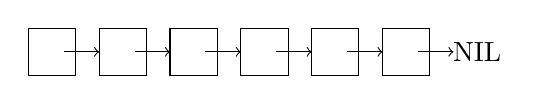
\begin{tikzpicture}[scale=3]
    \foreach \x in {-2, -1.7, ..., -0.4} {
      \draw (\x cm, 1cm) +(-0.1, -0.1) rectangle ++(0.1, 0.1);
      \draw[->] (\x cm, 1cm) +(0.05, 0) -- +(0.2, 0);
    }
    \draw (-0.2cm, 1cm) node {NIL};
    \end{tikzpicture}
  \caption{A list of nodes}
  \label{fig:list-example}
\end{figure}

Every node links to the next one or NIL. Linked-list is often defined through compound structure\footnote{In most cases, the data stored in list have the same type. However, there is also heterogeneous list, like the list in Lisp for example.}, for example:

\lstset{frame=single}
\begin{lstlisting}[language=Bourbaki]
struct List<A> {
    A key
    List<A> next
}
\end{lstlisting}

\index{List!empty} \index{List!empty testing}
It needs more clarification for the empty list. Many traditional environments support {\em null} concept. There are two different ways to represent empty list. One is to use null (or NIL) directly; the other is to construct a list, but put nothing as \texttt{[]}. From implementation perspective, null need not allocate any memory, while \texttt{[]} does. In this book, we use $\varnothing$ to represent generic empty list, set, or container.

\subsection{Access}
\index{List!head} \index{List!tail}
\index{List!Construction} \index{List!cons}
Given a none empty list $L$, we need define two functions to access its first element, and the rest sub-list. They are often called $first(L), rest(L)$ or $head(L), tail(L)$\footnote{They are named as \texttt{car} and \texttt{cdr} in Lisp due to the design of machine registers\cite{SICP}.}. On the other hand, we can construct a list from an element $x$ and another list $xs$ (can be empty), denoted as $x : xs$. It is also called the \texttt{cons} operation. We have the following equations hold:

\be
\begin{cases}
head(x:xs) & = x \\
tail(x:xs) & = xs
\end{cases}
\label{eq:list-head-tail}
\ee

For a none empty list $X$, we will also use $x_1$ for the first element, and use $X'$ for the rest sub-list. For example, when $X = [x_1, x_2, x_3, ...]$, then $X' = [x_2, x_3, ...]$.

\begin{Exercise}
\Question{For list of type $A$, suppose we can test if any two elements $x, y \in A$ are equal, define an algorithm to test if two lists are identical.}
\end{Exercise}

\section{Basic operations}
\index{List!length}
From the definition, we can count the length recursively: for empty list, the length is zero, otherwise, it is the length of the sub-list plus one.

\be
\begin{array}{rcl}
length(\nil) & = & 0 \\
length(L) & = & 1 + length(L')
\end{array}
\ee

In order to count the length, this algorithm traverses all the elements from head to end, hence it is bound to $O(n)$ time, where $n$ is the number of elements. To avoid repeatedly counting, we can also persist the length in a variable, and update it when mutate (add or delete) the list. Below is the iterative way to count length:

\begin{algorithmic}[1]
\Function{Length}{L}
  \State $n \gets 0$
  \While{$L \neq $ NIL}
    \State $n \gets n + 1$
    \State $L \gets $ \Call{Next}{$L$}
  \EndWhile
  \State \Return $n$
\EndFunction
\end{algorithmic}

We will also use notion $|L|$ for the length of list $L$ when the context is clear.

\subsection{index}
\index{List!index} \index{List!get at}
Different from array, which supports random access an element at position $i$ in constant time, we need traverse the list $i$ steps to access the target element.

\be
getAt(i,\ x:xs) = \begin{cases}
  i = 0: & x \\
  i \neq 0: & getAt(i - 1, xs) \\
\end{cases}
\ee

In order to get the $i$-th element from a none empty list:
\begin{itemize}
\item if $i$ is 0, the result is the first element;
\item Otherwise, the result is the $(i-1)$-th element in the sub-list.
\end{itemize}

We intend to leave the empty list not handled. The behavior when pass $\nil$ is undefined. As such, the out of bound case also leads to undefined behavior. If $i > |L|$ exceeds the length, we end up the edge case to access the $(i-|L|)$-th element of the empty list. On the other hand, if $i < 0$, minus it by one makes it even farther away from 0. We finally end up with the same situation that the index is negative, while the list is empty.

This algorithm is bound to $O(i)$ time as it advances the list $i$ steps. Below is the corresponding imperative implementation:

\begin{algorithmic}[1]
\Function{Get-At}{$i, L$}
  \While{$i \neq 0$}
    \State $L \gets $ \Call{Next}{$L$}  \Comment{Raise error when $L$ = NIL}
    \State $i \gets i - 1$
  \EndWhile
  \State \Return \Call{First}{$L$}
\EndFunction
\end{algorithmic}

\begin{Exercise}
\Question{In the iterative \textproc{Get-At}($i, L$) algorithm, what is the behavior when $L$ is empty? what is the behavior when $i$ is out of the bound or negative?}
\end{Exercise}

\subsection{Last}
\index{List!last} \index{List!init}
There is a pair of symmetric operations to `first/rest'. They are called `last/init'. For a none empty list $X = [x_1, x_2, ..., x_n]$, function $last$ returns the last element $x_n$, while $init$ returns the sub-list of $[x_1, x_2, ..., x_{n-1}]$. Although they are symmetric pairs left to right, `last/init' need linear time, because we need traverse the whole list to tail.


When access the last element of list $X$:
\begin{itemize}
\item If the $X$ contains only one element as $[x_1]$, then $x_1$ is the last one;
\item Otherwise, the result is the last element of the sub-list $X'$.
\end{itemize}

\be
\begin{array}{rcl}
last([x]) & = & x \\
last(x:xs) & = & last(xs) \\
\end{array}
\label{eq:list-last}
\ee

Similarly, when extract the sub-list of $X$ contains all elements without the last one:

\begin{itemize}
\item If $X$ is a singleton $[x_1]$, the result is empty $[\ ]$;
\item Otherwise, we recursively get the initial sub-list for $X'$, then prepend $x_1$ to it as the result.
\end{itemize}

\be
\begin{array}{rcl}
init([x]) & = & [\ ] \\
init(x:xs) & = & x : init(xs) \\
\end{array}
\ee

We leave the empty list not handled for both operations. The behavior is undefined if pass $\nil$ in. Below are the iterative implementation:

\begin{algorithmic}[1]
\Function{Last}{$L$}
  \State $x \gets $ NIL
  \While{$L \neq$ NIL}
    \State $x \gets $ \Call{First}{$L$}
    \State $L \gets $ \Call{Rest}{$L$}
  \EndWhile
  \State \Return $x$
\EndFunction
\Statex
\Function{Init}{$L$}
  \State $L' \gets $ NIL
  \While{\Call{Rest}{$L$} $\neq$ NIL} \Comment{Raise error when $L$ is NIL}
    \State $L' \gets$ \textproc{Cons}(\Call{First}{$L$}, $L'$)
    \State $L \gets $ \Call{Rest}{$L$}
  \EndWhile
  \State \Return \Call{Reverse}{$L'$}
\EndFunction
\end{algorithmic}

As advancing towards the tail, this algorithm accumulates the `init' result through `cons'. However, such result is in the reversed order. We need apply reverse (defined in section \ref{sec:reverse}) again to return the correct result. There is a question to ask if we can use `append' instead of `cons' in the exercise.

\subsection{Reverse index}
\index{List!Reverse index} \index{List!rindex}
$last$ is a special case of reverse index. The generic case is to find the last $i$-th element of a given list. The naive implementation takes two rounds of traverse: Determine the length $n$ through the first round; then access the $(n - i - 1)$-th element through the second round:

\be
  lastAt(i, L) = getAt(|L| - i - 1, L)
\ee

There actually exists better solution. The idea is to keep two pointers $p_1, p_2$ with the distance $i$ between them. The equation $rest^i(p_2) = p_1$ holds, where $rest^i(p_2)$ means repleatedly apply $rest()$ function $i$ times. When succeed $p_2$ by $i$ steps gets $p_1$. We start by pointing $p_2$ to the list head, and advance both pointers in parallel till $p_1$ arrives at tail. At that time point, $p_2$ exactly points to the $i$-th element from right. Figure \ref{fig:list-rindex} shows this idea. As $p_1, p_2$ form a window, this method is also called `sliding window' solution.

\begin{figure}[htbp]
  \centering
  \subcaptionbox{$p_2$ starts from the head, behind $p_1$ in $i$ steps.}{\includegraphics[scale=0.8]{img/list-rindex}} \\
  \subcaptionbox{When $p_1$ reaches the tail, $p_2$ points to the $i$-th element from right.}{\includegraphics[scale=0.8]{img/list-rindex-2}}
  \caption{Sliding window formed by two pointers}
  \label{fig:list-rindex}
\end{figure}

\begin{algorithmic}[1]
\Function{Last-At}{$i, L$}
  \State $p \gets L$
  \While{$i > 0$}
    \State $L \gets $ \Call{Rest}{$L$} \Comment{Raise error if out of bound}
    \State $i \gets i - 1$
  \EndWhile
  \While{\Call{Rest}{$L$} $\neq$ NIL}
    \State $L \gets$ \Call{Rest}{$L$}
    \State $p \gets$ \Call{Rest}{$p$}
  \EndWhile
  \State \Return \Call{First}{$p$}
\EndFunction
\end{algorithmic}

The functional implementation need special consideration as we cannot update pointers directly. Instead, we advance two lists $X = [x_1, x_2, ..., x_n]$ and $Y = [x_i, x_{i+1}, ..., x_n]$ simultaneously, where $Y$ is the sub-list without the first $i - 1$ elements.

\begin{itemize}
\item If $Y$ is a singleton list, i.e. $[x_n]$, then the last $i$-th element is the head of $X$;
\item Otherwise, we drop the first element from both $X$ and $Y$, then recursively check $X'$ and $Y'$.
\end{itemize}

\be
lastAt(i, X) = slide(X, drop(i, X))
\ee

where function $slide(X, Y)$ drops the heads for both lists:

\be
\begin{array}{rcl}
slide(x:xs,\ [y]) & = & x \\
slide(x:xs,\ y:ys) & = & slide(xs, ys) \\
\end{array}
\ee

Function $drop(m, X)$ discards the first $m$ elements from list $X$. It can be implemented by advancing $X$ by $m$ steps:

\be
\begin{array}{rcl}
drop(0,\ X) & = & X \\
drop(m,\ \nil) & = & \nil \\
drop(m,\ x:xs) & = & drop(m - 1, xs) \\
\end{array}
\ee

\begin{Exercise}
\Question{In the \textproc{Init} algorithm, can we use \textproc{Append}($L'$, \textproc{First}($L$)) instead of `cons'?}
\Question{How to handle empty list or out of bound index error in \textproc{Last-At} algorithm?}
\end{Exercise}

\subsection{Mutate}
\index{List!mutate}
Mutate operations include append, insert, update, and delete. Some functional environments actually implement mutate by creating a new list, while the original one is persisted for later reuse, or released at sometime (chapter 2 in \cite{okasaki-book}).

\subsubsection{Append}
\index{List!append}
Append is the symmetric operation of $cons$, it adds element on the tail instead of head. Because of this, it is also called `snoc'. For linked-list, it means we need traverse to the tail, hence it takes $O(n)$ time, where $n$ is the length. To avoid repeatedly traverse, we can record the tail reference as a variable, and keep updating it upon changes.

\be
\begin{array}{rcl}
append(\nil, x) & = & [x] \\
append(y:ys, x) & = & y : append(ys, x) \\
\end{array}
\ee

\begin{itemize}
\item If append $x$ to the empty list, the result is $[x]$;
\item Otherwise, we firstly recursive append $x$ to the rest sub-list, then prepend the original head to form the result.
\end{itemize}

The corresponding iterative implementation is as the following:

\begin{algorithmic}[1]
\Function{Append}{$L, x$}
  \If{$L = $ NIL}
    \State \Return \Call{Cons}{$x$, NIL}
  \EndIf
  \State $H \gets L$ \Comment{save the head}
  \While{\Call{Rest}{$L$} $\neq$ NIL}
    \State $L \gets$ \Call{Rest}{$L$}
  \EndWhile
  \State \Call{Rest}{$L$} $\gets$ \Call{Cons}{$x$, NIL}
  \State \Return $H$
\EndFunction
\end{algorithmic}

Update the \textproc{Rest} is typically implemented by setting the \texttt{next} reference field as shown in below example program.

\begin{lstlisting}[language=Bourbaki]
List<A> append(List<A> xs, T x) {
    if (xs == null) {
        return cons(x, null)
    }
    List<A> head = xs
    while (xs.next != null) {
        xs = xs.next
    }
    xs.next = cons(x, null)
    return head
}
\end{lstlisting}

\begin{Exercise}
\Question{Add a `tail' field in list definition, optimize the append algorithm to constant time.}
\Question{With the additional `tail' field, when need we update the tail variable? How does it affect the performance?}
\end{Exercise}

\subsubsection{Set value}
\index{List!set at}
Similar to $getAt$, we need advance to the target position, then change the element there. To define function $setAt(i, x, L)$:

\begin{itemize}
\item If $i = 0$, it means we are changing the first element, the result is $x : L'$;
\item Otherwise, we need recursively set the value at position $i-1$ for the sub-list $L'$.
\end{itemize}

\be
\begin{array}{rcl}
setAt(0, x,\ y:ys) & = & x : ys \\
setAt(i, x,\ y:ys) & = & y : setAt(i - 1, x, ys) \\
\end{array}
\ee

This algorithm is bound to $O(i)$ time, where $i$ is the position to update.

\begin{Exercise}
\Question{Handle the empty list and out of bound error for $setAt$.}
\end{Exercise}

\subsubsection{insert}
\index{List!insert} \index{List!insert at}
There are two different cases about insertion. One is to insert an element at a given position: $insert(i, x, L)$. The algorithm is similar to $setAt$; The other is to insert an element to a sorted list, and keep the order still sorted.

To insert $x$ at position $i$, we need firstly advance $i$ steps, then construct a new sub-list with $x$ as the head, then concatenate it to the first $i$ elements\footnote{$i$ starts from 0.}.

\begin{itemize}
\item If $i = 0$, it then turns to be a `cons' operation: $x : L$;
\item Otherwise, we recursively insert $x$ to $L'$ at position $i-1$; then prepend the original head.
\end{itemize}

\be
\begin{array}{rcl}
insert(0, x,\ L) & = & x : L \\
insert(i, x,\ y:ys) & = & x : insert(i - 1, x, ys) \\
\end{array}
\ee

When $i$ exceeds the list length, we can treat it as to append $x$. We leave this as an exercise. The following is the corresponding iterative implementation:

\begin{algorithmic}[1]
\Function{Insert}{$i, x, L$}
  \If{$i = 0$}
    \State \Return \Call{Cons}{$x, L$}
  \EndIf
  \State $H \gets L$
  \State $p \gets L$
  \While{$i > 0$ and $L \neq$ NIL}
    \State $p \gets L$
    \State $L \gets $ \Call{Rest}{$L$}
    \State $i \gets i - 1$
  \EndWhile
  \State \Call{Rest}{$p$} $\gets$ \Call{Cons}{$x, L$}
  \State \Return $H$
\EndFunction
\end{algorithmic}

If the list $L = [x_1, x_2, ..., x_n]$ is sorted, i.e. for any position $1 \leq i \leq j \leq n$, then $x_i \leq x_j$ holds. Here $\leq$ is abstract ordering. It can actually mean $\geq$ for descending order, or subset relationship etc. We can design the insert algorithm to maintain the sorted order. To insert element $x$ to a sorted list $L$:

\begin{itemize}
\item If either $L$ is empty or $x$ is not greater than the first element in $L$, we prepend $x$ to $L$ and returns $x : L$;
\item Otherwise, we recursively insert $x$ to the sub-list $L'$.
\end{itemize}

\be
\begin{array}{rcl}
insert(x,\ \nil) & = & [x] \\
insert(x,\ y : ys) & = & \begin{cases}
  x \leq y : & x : y : ys \\
  otherwise : & y : insert(x, ys) \\
  \end{cases}
\end{array}
\label{eq:list-ordered-insert}
\ee

Since the algorithm need compare elements one by one, it is bound to $O(n)$ time, where $n$ is the length. Below is the corresponding iterative implementation:

\begin{algorithmic}[1]
\Function{Insert}{$x, L$}
  \If{$L = $ NIL or $x <$ \Call{First}{$L$}}
    \State \Return \Call{Cons}{$x, L$}
  \EndIf
  \State $H \gets L$
  \While{\Call{Rest}{$L$} $\neq $ NIL and \textproc{First}(\Call{Rest}{$L$}) $< x$}
    \State $L \gets $ \Call{Rest}{$L$}
  \EndWhile
  \State \Call{Rest}{$L$} $\gets$ \textproc{Cons}($x$, \Call{Rest}{$L$})
  \State \Return $H$
\EndFunction
\end{algorithmic}

\label{sec:isort}
With this linear time ordered insertion defined, we can further develop the insertion-sort algorithm. The idea is to repeatedly insert elements to the empty list. Since each insert takes liner time, the overall sort is bound to $O(n^2)$.

\be
\begin{array}{rcl}
sort(\nil) & = & \nil \\
sort(x:xs) & = & insert(x, sort(xs)) \\
\end{array}
\ee

This is a recursive algorithm. It firstly sorts the sub-list, then inserts the first element in it. We can eliminate the recursion to develop a iterative implementation. The idea is to scan the list, and one by one insert them:

\begin{algorithmic}[1]
\Function{Sort}{$L$}
  \State $S \gets$ NIL
  \While{$L \neq$ NIL}
    \State $S \gets$ \textproc{Insert}(\Call{First}{$L$}, $S$)
    \State $L \gets$ \Call{Rest}{$L$}
  \EndWhile
  \State \Return $S$
\EndFunction
\end{algorithmic}

At any time during the loop, the result is sorted. There is a major difference between the recursive and the iterative implementations. The recursive one processes the list from right, while the iterative one is from left. We'll introduce `tail-recursion' in section \ref{sec:tail-call} to eliminate this difference. Chapter 3 introduces insertion sort in detail, including performance analysis and optimization.

\begin{Exercise}
\Question{Handle the out-of-bound case in insertion, and treat it as append.}
\Question{Design the insertion algorithm for array. When insert at position $i$, all elements after $i$ need shift to the end by one.}
\Question{Implement the insertion sort only with less than ($<$) defined.}
\end{Exercise}

\subsubsection{delete}
\index{List!delete} \index{List!delete at}
Symmetric to insert, delete also has two cases. One is to delete the element at a position; the other is to look up, then delete the element of a given value. The first case is defined as $delAt(i, L)$, the second case is defined as $delete(x, L)$.

To delete the element at position $i$, we need advance $i$ steps to the target position, then by pass the element, and link the rest sub-list.
\begin{itemize}
\item If $L$ is empty, then the result is empty too;
\item If $i = 0$, we are deleting the head, the result is $L'$;
\item Otherwise, recursively delete the $(i-1)$-th element from $L'$, then prepend the original head as the result.
\end{itemize}

\be
\begin{array}{rcl}
delAt(i,\ \nil) & = & \nil \\
delAt(0,\ x:xs) & = & xs \\
delAt(i,\ x:xs) & = & x : delAt(i - 1, xs) \\
\end{array}
\ee

This algorithm is bound to $O(i)$ as we need advance $i$ steps to perform deleting. Below is the iterative implementation:

\begin{algorithmic}[1]
\Function{Del-At}{$i, L$}
  \State $S \gets$ \Call{Cons}{$\perp, L$} \Comment{A sentinel node}
  \State $p \gets S$
  \While{$i > 0$ and $L \neq$ NIL}
    \State $i \gets i - 1$
    \State $p \gets L$
    \State $L \gets $ \Call{Rest}{$L$}
  \EndWhile
  \If{$L \neq$ NIL}
    \State \Call{Rest}{$p$} $\gets$ \Call{Rest}{$L$}
  \EndIf
  \State \Return \Call{Rest}{$S$}
\EndFunction
\end{algorithmic}

To simplify the implementation, we introduce a sentinel node $S$, it contains a special value $\perp$, and its next reference points to $L$. With $S$, we are save to cut-off any node in $L$ even for the first one. Finally, we return the list after $S$ as the result, and $S$ itself can be discarded.

For the `find and delete' case, there are two options. We can either find and delete the first occurrence of a value; or remove all the occurrences. The later is more generic, we leave it as an exercise. When delete $x$ from list $L$:

\begin{itemize}
\item If the list is empty, the result is $\nil$;
\item Otherwise, we compare the head and $x$, if they are equal, then the result is $L'$;
\item If the head does not equal to $x$, we keep the head, and recursively delete $x$ in $L'$.
\end{itemize}

\be
\begin{array}{rcl}
delete(x,\ \nil) & = & \nil \\
delete(x,\ y:ys) & = & \begin{cases}
  x = y : & ys \\
  x \neq y : & y : delete(x, ys) \\
  \end{cases} \\
\end{array}
\label{eq:list-delete}
\ee

This algorithm is bound to $O(n)$ time, where $n$ is the length, as it need scan the list to find the target element. For the iterative implementation, we also introduce a sentinel node to simplify the logic:

\begin{algorithmic}[1]
\Function{Delete}{$x, L$}
  \State $S \gets$ \Call{Cons}{$\perp, L$}
  \State $p \gets$ L
  \While{$L \neq$ NIL and \Call{First}{$L$} $\neq x$}
    \State $p \gets L$
    \State $L \gets$ \Call{Rest}{$L$}
  \EndWhile
  \If{$L \neq$ NIL}
    \State \Call{Rest}{$p$} $\gets$ \Call{Rest}{$L$}
  \EndIf
  \State \Return \Call{Rest}{$S$}
\EndFunction
\end{algorithmic}

\begin{Exercise}
\Question{Design the algorithm to find and delete all occurrences of a given value.}
\Question{Design the delete algorithm for array, all elements after the delete position need shift to front by one.}
\end{Exercise}

\subsubsection{concatenate}
\label{concat} \index{List!concat}
Append is a special case for concatenation. Append only adds one element, while concatenation adds multiple ones. However, the performance would be quadratic if repeatedly appending as below:

\be
\begin{array}{rcl}
X \doubleplus \nil & = & X \\
X \doubleplus (y:ys) & = & append(X, y) \doubleplus ys \\
\end{array}
\ee

In this implementation when concatenate $X$ and $Y$, each append operation traverses to the tail, and we do this for $|Y|$ times. the total time is bound to $O(|X| + (|X| + 1) + ... + (|X| + |Y|)) = O(|X||Y| + |Y|^2)$. Consider the link (cons) operation is fast (constant time), we can traverse to the tail of $X$ only once, then link $Y$ to the tail.

\begin{itemize}
\item If $X$ is empty, the result is $Y$;
\item Otherwise, we concatenate the sub-list $X'$ with $Y$, then prepend the head as the result.
\end{itemize}

We can further improve it a bit: when $Y$ is empty, we needn't traverse, but directly return $X$:

\be
\begin{array}{rcl}
\nil \doubleplus Y & = & Y \\
X \doubleplus \nil & = & X \\
(x:xs) \doubleplus Y & = & x : (xs \doubleplus Y) \\
\end{array}
\ee

The modified algorithm only traverse list $X$, then link its tail to $Y$, hence it is bound $O(|X|)$ time. In imperative settings, concatenation can be realized in constant time with the additional tail variable. We leave its implementation as exercise. Below is the iterative implementation without using the tail variable:

\begin{algorithmic}[1]
\Function{Concat}{$X, Y$}
  \If{$X = $ NIL}
    \State \Return $Y$
  \EndIf
  \If{$Y = $ NIL}
    \State \Return $X$
  \EndIf
  \State $H \gets X$
  \While{\Call{Rest}{$X$} $\neq$ NIL}
    \State $X \gets$ \Call{Rest}{$X$}
  \EndWhile
  \State \Call{Rest}{$X$} $\gets Y$
  \State \Return $H$
\EndFunction
\end{algorithmic}

\subsection{sum and product}
\index{List!sum} \index{List!product}
It is common to calculate the sum or product of a list of numbers. They have almost same structure. We will introduce how to abstract them to higher order computation in section \ref{sec:fold}.

\subsubsection{Recursive sum and product}

To calculate the sum of a list:

\begin{itemize}
\item If the list is empty, the result is zero;
\item Otherwise, the result is the first element plus the sum of the rest.
\end{itemize}

\be
\begin{array}{rcl}
sum(\nil) & = & 0 \\
sum(x:xs) & = & x + sum(xs) \\
\end{array}
\ee

We can't merely replace $+$ to $\times$ to obtain product algorithm, because it always returns zero. We need define the product of the empty list as 1.

\be
\begin{array}{rcl}
product(\nil) & = & 1 \\
product(x:xs) & = & x \cdot product(xs) \\
\end{array}
\ee

Both algorithms traverse the list, hence are bound to $O(n)$ time, where $n$ is the length.

\subsubsection{Tail call recursion}
\index{Tail call} \index{Tail recursion} \index{Tail recursive call}
\label{sec:tail-call}
Both sum and product algorithms calculate from right to left. We can change them to calculate the {\em accumulated} result from left to right. For sum, it accumulates from 0, then adds element one by one; while for product, it starts from 1, then repeatedly multiplying elements. The accumulate process can be defined as:

\begin{itemize}
\item If the list is empty, return the accumulated result;
\item Otherwise, accumulate the first element to the result, then go on accumulating.
\end{itemize}

Below are the accumulated sum and product:

\be
\begin{array}{cc}
  \begin{array}{rl}
  sum'(A,\ \nil) = & A \\
  sum'(A,\ x:xs) = & sum(x + A, xs) \\
  \end{array}
  &
  \begin{array}{rl}
  prod'(A,\ \nil) = & A \\
  prod'(A,\ x:xs) = & prod'(x \cdot A, xs) \\
  \end{array} \\
\end{array}
\ee

Given a list, we can call $sum'$ with 0, and $prod'$ with 1:

\be
sum(X) = sum'(0, X)
\quad \quad \quad
product(X) = prod'(1, X)
\ee

Or merely simplify it to Curried form:

\[
sum = sum'(0) \quad \quad \quad product = prod'(1)
\]

\index{Curried Form} \index{Currying}
Curried form was introduced by Schönfinkel (1889 - 1942) in 1924, then widely used by Haskell Curry from 1958. It is known as {\em Currying}\cite{slpj-book-1987}. For a function taking 2 parameters $f(x, y)$, when pass one argument $x$, it ends up to another function of $y$: $g(y) = f(x, y)$ or $g = f\ x$. We can further extend it to multiple variables, that $f(x, y, ..., z)$ can be Curried to a series of functions: $f, f\ x, f\ x\ y, ...$. No matter how many variables, we can treat them as a series of Curried function, each has only one parameter: $f(x, y, ..., z) = f(x)(y)...(z) = f\ x\ y\ ...\ z$.

The accumulated sum does not only calculate the result from left to right, it needn't book keeping any context, state, or intermediate result for recursion. All such states are either passed as argument (i.e. $A$), or can be dropped (the previous element in the list). Such recursive calls are often optimized as pure loops in practice. We call this kind of function as {\em tail recursion} (or `tail call'), and the optimization to eliminate recursion is called 'tail recursion optimization'\cite{wiki-tail-call}, because the recursion happens at the tail place in the function. The performance of tail call can be greatly improved after optimization, and we can avoid the issue of stack overflow in deep recursions.

In section \ref{sec:isort} about insertion sort, we mentioned the recursive algorithm sorts elements form right. We can also optimize it to tail call:

\be
\begin{array}{rcl}
sort'(A,\ \nil) & = & A \\
sort'(A,\ x:xs) & = & sort'(insert(x, A), xs) \\
\end{array}
\ee

And the sort is defined in Curried form with $\nil$ as the start value:

\be
sort = sort'(\nil)
\ee

As a typical tail call problem, let's consider how to compute $b^n$ effectively? (refer to problem 1.16 in \cite{SICP}.) A brute-force solution is to repeatedly multiplying $b$ for $n$ times from 1. This algorithm is bound to $O(n)$:

\begin{algorithmic}[1]
\Function{Pow}{$b, n$}
  \State $x \gets 1$
  \Loop{ $n$ times}
    \State $x \gets x \cdot b$
  \EndLoop
  \State \Return $x$
\EndFunction
\end{algorithmic}

Actually, the solution can be greatly improved. When compute $b^8$, after the first 2 loops, we get $x = b^2$. At this stage, we
needn't multiply $x$ with $b$ to get $b^3$, but directly compute $x^2$, which gives $b^4$. If do this again, we get $(b^4)^2 = b^8$. Thus we only need loop 3 times, but not 8 times.

Based on this idea, if $n = 2^m$ for some none negative integer $m$, we can design below algorithm to compute $b^n$:

\[
\begin{array}{rcl}
b^1 & = & b \\
b^n & = & (b^{\frac{n}{2}})^2 \\
\end{array}
\]

We next extend this divide and conquer method for any none negative integer $n$:

\begin{itemize}
\item If $n = 0$, define $b^0 = 1$;
\item If $n$ is even, we halve $n$, to compute $b^{\frac{n}{2}}$. Then square it;
\item Otherwise $n$ is odd. Since $n-1$ is even, we recursively compute $b^{n-1}$, the multiply $b$ atop it.
\end{itemize}

\be
\begin{array}{rcl}
b^0 & = & 1 \\
b^n & = & \begin{cases}
2 | n : & (b^{\frac{n}{2}})^2 \\
otherwise : & b \cdot b^{n-1} \\
\end{cases}
\end{array}
\ee

However, the 2nd clause blocks us to turn it tail recursive. Alternatively, we can square the base number, and halve the exponent.

\be
\begin{array}{rcl}
b^0 & = & 1 \\
b^n & = & \begin{cases}
2 | n : & (b^2)^{\frac{n}{2}} \\
otherwise : & b \cdot b^{n-1} \\
\end{cases}
\end{array}
\ee

With this change, we can develop a tail recursive algorithm to compute $b^n = pow(b, n, 1)$.

\be
\begin{array}{rcl}
pow(b, 0, A) & = & A \\
pow(b, n, A) & = & \begin{cases}
  2 | n : & pow(b^2, \dfrac{n}{2}, A) \\
  otherwise: & pow(b, n - 1, b \cdot A) \\
\end{cases}
\end{array}
\ee

Compare to the brute-force implementation, this one improves to $O(\lg n)$ time. Actually, we can improve it further. If represent $n$ in binary format $n = (a_ma_{m-1}...a_1a_0)_2$, we clearly know that the computation for $b^{2^i}$ is necessary if $a_i = 1$. This is quite similar to the idea of Binomial heap (\autoref{sec:binomial-heap}). We can multiplying all of them for bits of 1.

For example, when compute $b^{11}$, as $11 = (1011)_2 = 2^3 + 2 +1$, thus $b^{11} = b^{2^3} \times b^2 \times b$. We get the result by these steps:

\begin{enumerate}
\item calculate $b^1$, which is $b$;
\item Square to $b^2$ from the previous result;
\item Square again to $b^{2^2}$ from step 2;
\item Square to $b^{2^3}$ from step 3.
\end{enumerate}

Finally, we multiply the result of step 1, 2, and 4 to get $b^{11}$. Summarize this idea, we improve the algorithm as below.

\be
\begin{array}{rcl}
pow(b, 0, A) & = & A \\
pow(b, n, A) & = & \begin{cases}
  2 | n : & pow(b^2, \dfrac{n}{2}, A) \\
  otherwise: & pow(b^2, \lfloor \dfrac{n}{2} \rfloor, b \cdot A) \\
  \end{cases}
\end{array}
\ee

This algorithm essentially shifts $n$ to right 1 bit each time (divide $n$ by 2). If the LSB (Least Significant Bit, the lowest) is 0, $n$ is even. It squares the base and keeps the accumulator $A$ unchanged; If the LSB is 1, $n$ is odd. It squares the base and accumulates it to $A$; When $n$ is zero, we exhaust all bits, $A$ is the final result. At any time, the updated base number $b'$, the shifted exponent number $n'$, and the accumulator $A$ satisfy the invariant $b^n = A \cdot (b')^{n'}$.

Compare to previous implementation, which minus by one for odd $n$, this algorithm halves $n$ every time. It exactly runs $m$ rounds, where $m$ is the number of bits. We leave the imperative implementation as exercise.

Back to the sum and product. The iterative implementation applies plus and multiply while traversing:

\begin{algorithmic}[1]
\Function{Sum}{$L$}
  \State $s \gets 0$
  \While{$L \neq$ NIL}
    \State $s \gets s +$ \Call{First}{$L$}
    \State $L \gets$ \Call{Rest}{$L$}
  \EndWhile
  \State \Return $s$
\EndFunction
\Statex
\Function{Product}{$L$}
  \State $p \gets 1$
  \While{$L \neq$ NIL}
    \State $p \gets p\ \cdot$ \Call{First}{$L$}
    \State $L \gets$ \Call{Rest}{$L$}
  \EndWhile
  \State \Return $p$
\EndFunction
\end{algorithmic}

One interesting usage of product is to calculate factorial of $n$ as: $n! = product([1..n])$.

\subsection{maximum and minimum}
\index{List!maximum} \index{List!minimum}

For a list of comparable elements (we can define order for any two elements), there is the maximum and minimum. The algorithm structure of $max/min$ is same. For a none empty list:

\begin{itemize}
\item If there is only one element (a singleton) $[x_1]$, the result is $x_1$;
\item Otherwise, we recursively find the min/max of the sub-list, then compare it with the first element to determine the result.
\end{itemize}

\be
  \begin{array}{rcl}
  min([x]) & = & x \\
  min(x:xs) & = & \begin{cases}
    x < min(xs) : & x \\
    otherwise: & min(xs) \\
  \end{cases}
  \end{array}
\ee
and
\be
  \begin{array}{rcl}
  max([x]) & = & x \\
  max(x:xs) & = & \begin{cases}
    x > max(xs) : & x \\
    otherwise: & max(xs) \\
  \end{cases}
  \end{array}
\ee

Both process the list from right to left. We can modify them to tail recursive. It also brings us the `on-line' feature, that at any time, the accumulator is the min/max so far processed. Use $min$ for example:

\be
\begin{array}{rcl}
min'(a,\ \nil) & = & a \\
min'(a,\ x:xs) & = & \begin{cases}
  x < a : & min'(x, xs) \\
  otherwise : & min'(a, xs) \\
  \end{cases}
\end{array}
\ee

Different from $sum'/prod'$, we can't pass a fixed starting value to the tail recursive $min'/max'$, unless we use $\pm \infty$ in below Curried form:

\[
  min = min'(\infty) \quad \quad \quad max = max'(- \infty)
\]

Alternatively, we can pass the first element as the accumulator given min/max only takes none empty list:

\be
  min(x:xs) = min'(x,\ xs)
  \quad \quad \quad
  max(x:xs) = max'(x,\ xs)
\ee

The optimized tail recursive algorithm can be further changed to purely iterative implementation. We give the \textproc{Min} example, and skip \textproc{Max}.

\begin{algorithmic}[1]
\Function{Min}{$L$}
  \State $m \gets$ \Call{First}{$L$}
  \State $L \gets$ \Call{Rest}{$L$}
  \While{$L \neq$ NIL}
    \If{\Call{First}{$L$} $< m$ }
      \State $m \gets$ \Call{First}{$L$}
    \EndIf
    \State $L \gets$ \Call{Rest}{$L$}
  \EndWhile
  \State \Return $m$
\EndFunction
\end{algorithmic}

There is a way to realize the tail recursive algorithm without using accumulator explicitly. The idea is to re-use the first element as the accumulator. Every time, we compare the head with the next element; then drop the greater one for $min$, and drop the less one for $max$.

\be
\begin{array}{rcl}
min([x]) & = & x \\
min(x_1:x_2:xs) & = & \begin{cases}
  x_1 < x_2 : & min(x_1:xs) \\
  otherwise: & min(x_2:xs) \\
  \end{cases}
\end{array}
\ee

We skip the definition for $max$ as it is symmetric.

\begin{Exercise}
\Question{Change the $length$ to tail call.}
\Question{Change the insertion sort to tail call.}
\Question{Implement the $O(\lg n)$ algorithm to calculate $b^n$ by represent $n$ in binary.}
\end{Exercise}

\section{Transform}
\index{List!Transform}
From algebraic perspective, there are two types of transform: one keeps the list structure, but only change the elements; the other alter the list structure, hence the result is not isomorphic to the original list. Particularly, we call the former {\em map}.

\subsection{map and for-each}
\index{List!map}
The first example is to convert a list of numbers to their represented strings, like to change [3, 1, 2, 4, 5] to [``three'', ``one'', ``two'', ``four'', ``five'']

\be
\begin{array}{rcl}
toStr(\nil) & = & \nil \\
toStr(x:xs) & = & str(x) : toStr(xs) \\
\end{array}
\label{eq:tostr}
\ee

For the second example, consider a dictionary, which is a list of words grouped by initial letter. Like:

\begin{verbatim}
[[a, an, another, ... ],
 [bat, bath, bool, bus, ...],
 ...,
 [zero, zoo, ...]]
\end{verbatim}

Next we process a text ({\em Hamlet} for example), and augment each word with their number of occurrence, like:

\begin{verbatim}
[[(a, 1041), (an, 432), (another, 802), ... ],
 [(bat, 5), (bath, 34), (bool, 11), (bus, 0), ...],
 ...,
 [(zero 12), (zoo, 0), ...]]
\end{verbatim}

Now for every initial letter, we want to figure out which word occurs most. How to write a program to do this work? The output is a list of words, that every one has the most occurrences in the group, something like \texttt{[a, but, can, ...]}. We need develop a program that transform \textbf{a list of groups of word-number pairs} into \textbf{a list of words}.

First, we need define a function. It takes a list of word-number pairs, finds the word paired with the biggest number. Sort is overkill. What we need is a special max function $maxBy(cmp, L)$, where $cmp$ compares two elements abstractly.

\be
\begin{array}{rcl}
maxBy(cmp,\ [x]) & = & x \\
maxBy(cmp,\ x_1 : x_2 : xs) & = & \begin{cases}
  cmp(x_1, x_2) : & maxBy(cmp, x_2 : xs) \\
  otherwise : & maxBy(cmp, x_1 : xs) \\
  \end{cases}
\end{array}
\ee

For a pair $p = (a, b)$ we define two access functions:

\be
\begin{cases}
fst\ (a, b) = & a \\
snd\ (a, b) = & b \\
\end{cases}
\ee

Instead of embedded parenthesis $fst((a, b)) = a$, we omit one layer, and use a space. Generally, we treat $f\ x = f(x)$ when the context is clear. Then we can define a special compare function for word-count pairs:

\be
less(p_1, p_2) = snd(p_1) < snd(p_2)
\ee

Then pass $less$ to $maxBy$ to finalize our definition (in Curried form):

\be
max'' = maxBy(less)
\ee

With $max''()$ defined, we can develop the solution to process the whole list.

\be
\begin{array}{rcl}
solve(\nil) & = & \nil \\
solve(x:xs) & = & fst(max''(x)) : solve(xs) \\
\end{array}
\label{eq:solve}
\ee

\subsubsection{Map}
\index{List!map}

The $solve()$ and $toStr()$ functions reveal the same structure, although they are developed for different problems. We can abstract this common structure as {\em map}:

\be
\begin{array}{rcl}
map(f,\ \nil) & = & \nil \\
map(f,\ x:xs) & = & f(x) : map(f, xs) \\
\end{array}
\ee

$map$ takes the function $f$ as argument, applies it to every element to form a new list. A function that computes with other functions is called {\em high-order} function. If the type of $f$ is $A \to B$, which means it sends an element of $A$ to the result of $B$, then the type of map is:

\be
map :: (A \to B) \to [A] \to [B]
\ee

We read it as: map takes a function of $A \to B$, then convert a list $[A]$ to another list $[B]$. The two examples in previous section can be defined with map as (in Curried form):

\[
\begin{array}{l}
toStr  = map\ str \\
solve = map \ (fst \circ max'')
\end{array}
\]

Where $f \circ g$ means function composite, i.e. first apply $g$ then apply $f$. $(f \circ g)\ x = f(g(x))$, Read as $f$ after $g$. Map can also be defined from the domain theory point of view. Function $y = f(x)$ defines the map from $x$ in set $X$ to $y$ in set $Y$:

\be
Y = \{ f(x) | x \in X \}
\ee

This type of set definition is called Zermelo-Frankel set abstraction (known as ZF expression) \cite{algo-fp}. The different
is that the mapping is from a list (but not set) to another: $Y = [f(x) | x \in Y]$. There can be duplicated elements. For list, such ZF style expression is called {\em list comprehension}.

List comprehension is a powerful tool. As an example, let us see how to realize the permutation algorithm. Extend from generating all-permutations as \cite{algo-fp} and \cite{erlang}, we define a generic $perm(L, r)$, that permutes $r$ out of the total $n$ elements in the list $L$. There are total $P_n^r = \dfrac{n!}{(n-r)!}$ solutions.

\be
perm(L, r) = \begin{cases}
  |L| < r\ \text{or}\ r = 0: & [[\ ]] \\
  otherwise: & [x:ys\ |\ x \in L, ys \in perm(delete(x,L), r-1)] \\
  \end{cases}
\ee

If pick zero element for permutation, or there are too few (less than $r$), the result is a list of empty list; otherwise, we recursively pick $r-1$ out of the rest $n-1$ elements; then prepend $x$ before each. Below Haskell example program utilizes the list comprehension feature:

\begin{Haskell}
perm xs r | r == 0 || length xs < r = [[]]
          | otherwise = [ x:ys | x <-xs,
                                 ys <- perm (delete x xs) (r-1)]
\end{Haskell}

For the iterative \textproc{Map} implementation, below algorithm uses a sentinel node to simplify the logic to handle head reference.

\begin{algorithmic}[1]
\Function{Map}{$f, L$}
  \State $L' \gets$ \Call{Cons}{$\perp$, NIL} \Comment{Sentinel node}
  \State $p \gets L'$
  \While{$L \neq$ NIL}
    \State $x \gets$ \Call{First}{$L$}
    \State $L \gets$ \Call{Rest}{$L$}
    \State \Call{Rest}{$p$} $\gets$ \Call{Cons}{$f(x)$, NIL}
    \State $p \gets$ \Call{Rest}{$p$}
  \EndWhile
  \State \Return \Call{Rest}{$L'$} \Comment{Drop the sentinel}
\EndFunction
\end{algorithmic}

\subsubsection{For each}
\index{List!for each}

Sometimes we only need to traverse the list, repeatedly process the elements one by one without building the new list. Here is an example that print every element out:

\begin{algorithmic}[1]
\Function{Print}{$L$}
  \While{$L \neq$ NIL}
    \State print \Call{First}{$L$}
    \State $L \gets$ \Call{Rest}{$L$}
  \EndWhile
\EndFunction
\end{algorithmic}

More generally, we can pass a procedure $P$, then traverse the list and apply $P$ to each element.

\begin{algorithmic}[1]
\Function{For-Each}{$P, L$}
  \While{$L \neq$ NIL}
    \State \textproc{P}(\Call{First}{$L$})
    \State $L \gets$ \Call{Rest}{$L$}
  \EndWhile
\EndFunction
\end{algorithmic}

\subsubsection{Examples}

As an example, let's see a ``$n$-lights puzzle''\cite{poj-drunk-jailer}. There are $n$ lights in a room, all of them are off. We execute the following $n$ rounds:

\begin{enumerate}
\item Switch all the lights in the room (all on);
\item Switch lights with number 2, 4, 6, ... , that every other light is switched, if the light is on, it will be off;
\item Switch every third lights, number 3, 6, 9, ... ;
\item ...
\end{enumerate}

And at the last round, only the last light (the $n$-th light) is switched. The question is how many lights are on in the end?

Let's start with a brute-force solution, then improve it step by step. We represent the state of $n$ lights as a list of 0/1 numbers. 0 is off, 1 is on. The initial state are all zeros: [0, 0, ..., 0]. We label the light from 1 to $n$, then map them to ($i$, on/off) pairs:

\[
lights = map(i \mapsto (i, 0),\ [1, 2, 3, ... n])
\]

It binds each number to zero, the result is a list of pairs: $L = [(1, 0), (2, 0), ..., (n, 0)]$. Next we operate this list of pairs for $n$ rounds. In the $i$-th round, switch the second value in this pair if its label is divided by $i$. Consider $1 - 0 = 1$, and $1 - 1 = 0$, we can switch 0/1 value of $x$ by $1 - x$. For light $(j, x)$, if $i | j$, (i.e. $j \bmod i = 0$), then switch, otherwise leave the light untouched.

\be
switch(i, (j, x)) = \begin{cases}
  j \bmod i = 0 : & (j, 1 - x) \\
  otherwise: & (j, x) \\
  \end{cases}
\ee

The $i$-th round for all lights can be realized as map:

\be
map(switch(i), L)
\ee

Here we use the Curried form of $switch$, which is equivalent to:

\[
map((j, x) \mapsto switch(i, (j, x)), L)
\]

Next, we define a function $op()$, which performs above mapping on $L$ over and over by $n$ rounds. We call this function with $op([1, 2, ..., n], L)$.

\be
\begin{array}{rcl}
op(\nil,\ L) & = & L \\
op(i:is,\ L) & = & op(is, map(switch(i), L)) \\
\end{array}
\ee

At this stage, we can sum the second value of each pair in list $L$ to get the answer.

\be
solve(n) = sum(map(snd, op([1, 2, ..., n], lights)))
\ee

Below is the example Haskell implementation of this brute-force solution:

\begin{Haskell}
solve = sum . (map snd) . proc  where
    lights = map (\i -> (i, 0)) [1..n]
    proc n = operate [1..n] lights
    operate [] xs = xs
    operate (i:is) xs = operate is (map (switch i) xs)

switch i (j, x) = if j `mod` i == 0 then (j, 1 - x) else (j, x)
\end{Haskell} %$

Run this program from 1 light to 100 lights, let's see what the answers are (we added line breaks):

\begin{verbatim}
[1,1,1,
 2,2,2,2,2,
 3,3,3,3,3,3,3,
 4,4,4,4,4,4,4,4,4,
 5,5,5,5,5,5,5,5,5,5,5,
 6,6,6,6,6,6,6,6,6,6,6,6,6,
 7,7,7,7,7,7,7,7,7,7,7,7,7,7,7,
 8,8,8,8,8,8,8,8,8,8,8,8,8,8,8,8,8,
 9,9,9,9,9,9,9,9,9,9,9,9,9,9,9,9,9,9,9,10]
\end{verbatim}

This result is interesting:

\begin{itemize}
\item the first 3 answers are 1;
\item the 4-th to the 8-th answers are 2;
\item the 9-th to the 15-th answers are 3;
\item ...
\end{itemize}

It seems that the $i^2$-th to the $((i+1)^2-1)$-th answers are $i$. Actually, we can prove it:

\begin{proof}
Given $n$ lights labeled from 1 to $n$, consider which lights are on finally. Since the initial states for all lights are off, we can say that, the lights which are manipulated odd times are on. For every light $i$, it will be switched at the $j$ round if $i$ can be divided by $j$ (denote as $j | i$). Only the lights which have odd number of factors are on in the end.

The key point to solve this puzzle, is to find all numbers which have odd number of factors. For any positive integer $n$, let $S$ be the set of all factors of $n$. $S$ is initialized to $\varnothing$. If $p$ is a factor of $n$, there must exist a positive integer $q$ such that $n = p q$ holds. It means $q$ is also a factor of $n$. We add 2 different factors to set $S$ if and only if $p \neq q$, which keeps $|S|$ even all the time unless $p = q$. In such case, $n$ is a square number. We can only add 1 factor to set $S$, which leads to odd number of factors.
\end{proof}

At this stage, we can design a fast solution by finding the number of square numbers under $n$.

\be
solve(n) = \lfloor \sqrt{n} \rfloor
\ee

Below Haskell example program outputs the answer for 1, 2, ..., 100 lights:

\begin{Haskell}
map (floor . sqrt) [1..100]
\end{Haskell}

Map is a generic concept does not limit to list. It can be applied to many complex algebraic structures. The next chapter about binary search tree explains how to map on trees. As long as we can traverse the structure, and the empty is defined, we can use the same mapping idea.

\subsection{reverse}
\index{List!reverse} \label{sec:reverse}
It's a classic exercise to reverse a singly linked-list with minimum space. One must carefully manipulate the node reference, however, there exists easy method to implement reverse:

\begin{enumerate}
\item Write a purely recursive solution;
\item Change it to tail-call;
\item Translate the tail-call solution to imperative operations.
\end{enumerate}

The purely recursive solution is straightforward. To reverse a list $L$.

\begin{itemize}
\item If $L$ is empty, the reversed result is empty;
\item Otherwise, recursively reverse sub-list $L'$, then append the first element to the end.
\end{itemize}

\be
\begin{array}{rcl}
reverse(\nil) & = & \nil \\
reverse(x:xs) & = & append(reverse(xs), x) \\
\end{array}
\ee

However, the performance is poor. As it need traverse to the end to append, this algorithm is bound to quadratic time. We can optimize it with tail call, use an accumulator to store the reversed part so far. We initialize the accumulator as empty: $reverse = reverse'(\nil)$.

\be
\begin{array}{rcl}
reverse'(A,\ \nil) & = & A \\
reverse'(A,\ x:xs) & = & reverse'(x:A,\ xs) \\
\end{array}
\ee

Different from appending, cons (:) is a constant time operation. The idea is to repeatedly take the elements from the head, and prepend them to the accumulator. It essentially likes to store elements in a stack, then pop them out. The overall performance is $O(n)$, where $n$ is the length. Since tail call need not keep the context, we can optimize it to purely iterative loops:

\begin{algorithmic}[1]
\Function{Reverse}{$L$}
  \State $A \gets$ NIL
  \While{$L \neq$ NIL}
    \State $A \gets $ \textproc{Cons}(\Call{First}{$L$}, $A$)
    \State $L \gets$ \Call{Rest}{$L$}
  \EndWhile
  \State \Return $A$
\EndFunction
\end{algorithmic}

However, this algorithm creates a new reversed list, but not mutate the original one. We need change it to in-place mutate $L$ as the below example program:

\begin{lstlisting}[language=Bourbaki]
List<T> reverse(List<T> xs) {
  List<T> p, ys = null
  while (xs != null) {
    p = xs
    xs = xs.next
    p.next = ys
    ys = p
  }
  return ys
}
\end{lstlisting}

\begin{Exercise}
\Question{Given a number from 0 to 1 billion, write a program to give its English representation. For e.g. 123 is `one hundred and twenty three'. What if there is decimal part?}
\Question{Implement the algorithm to find the maximum value in a list of pairs $[(k, v)]$ in tail call.}
\end{Exercise}

\section{Sub-list}
\index{List!Extract sub-list}
Different from array which is capable to slice a continuous segment fast, it typically need linear time to traverse and extract sub-list.

\subsection{take, drop, and split-at}
\index{List!take} \index{List!drop} \index{List!split at}

Taking the first $n$ elements is essentially to slice the list from 1 to $n$: $sublist(1, n, L)$. If either $n = 0$ or $L = \nil$, the sub-list is empty; otherwise, we recursively take the first $n - 1$ elements from the $L'$, then prepend the first element.

\be
\begin{array}{rcl}
take(0, L) & = & \nil \\
take(n, \nil) & = & \nil \\
take(n, x:xs) & = & x : take(n - 1, xs) \\
\end{array}
\ee

This algorithm handles the out of bound case like this: if $n > |L|$ or $n$ is negative, it ends up to the edge case that $L$ becomes empty, hence returns the whole list as the result.

Drop, on the other hand, discards the first $n$ elements and returns the rest. It is equivalent to slice the sub-list from right: $sublist(n + 1, |L|, L)$, where $|L|$ is the length. Its implementation is symmetric:

\be
\begin{array}{rcl}
drop(0, L) & = & L \\
drop(n, \nil) & = & \nil \\
drop(n, x:xs) & = & drop(n - 1, xs) \\
\end{array}
\ee

We leave the imperative implementation for $take/drop$ as exercise. As the next step, we can develop a algorithm to extract sub-list at any position for a given length:

\be
sublist(from, cnt, L) = take(cnt, drop(from - 1, L))
\ee

Or slice the list with left and right boundaries:

\be
slice(from, to, L) = drop(from - 1, take(to, L))
\ee

\index{List!split at}
The boundary is defined as $[from, to]$. It includes both ends. We can also split a list at a given position:

\be
splitAt(i, L) = (take(i, L), drop(i, L))
\label{eq:split-at}
\ee

\begin{Exercise}
\Question{Define $sublist$ and $slice$ in Curried Form without $L$ as parameter.}
\end{Exercise}

\subsubsection{conditional take and drop}
\index{List!take while} \index{List!drop while}
Instead of specifying number of elements for $take/drop$, one may want to provide a predication. We keep taking or dropping as far as the condition meets. We define such algorithm as $takeWhile/dropWhile$.

$takeWhile/dropWhile$ examine elements one by one against the prediction. They ignore the rest even if some elements satisfy the condition. We'll see this different in the section of filtering.

\be
\begin{array}{rcl}
takeWhile(p,\ \nil) & = & \nil \\
takeWhile(p,\ x:xs) & = & \begin{cases}
  p(x) : & x : takeWhile(p, xs) \\
  otherwise: & \nil \\
  \end{cases}
\end{array}
\ee

Where $p$ is the prediction. When applied to an element, $p$ returns true or false to indicate the condition is satisfied. $dropWhile$ is symmetric:

\be
\begin{array}{rcl}
dropWhile(p,\ \nil) & = & \nil \\
dropWhile(p,\ x:xs) & = & \begin{cases}
  p(x) : & dropWhile(p, xs) \\
  otherwise: & x:xs \\
  \end{cases}
\end{array}
\ee

\subsection{break and group}
Break and group are operations to re-arrange a list into multiple sub-lists. They typically perform the re-arrangement while traverse the list to keep the performance linear.

\subsubsection{break and span}
\index{List!break} \index{List!span}

$break/span$ can be considered as a general form of splitting. Instead of splitting at a given position, $break/span$ scans elements with a prediction. It extracts the longest prefix of the list against the condition, and returns it together with the rest as a pair.

There are two different cases. For a given predication, one is to pick the elements satisfied; the other is to pick the elements not satisfied. The former is called $span$, the later is called $break$.

\be
\begin{array}{rcl}
span(p,\ \nil) & = & (\nil, \nil) \\
span(p,\ x:xs) & = & \begin{cases}
  p(x) : & (x : A,\ B)\ \text{where}\ (A, B) = span(p, xs) \\
  otherwise : & (\nil,\ x:xs) \\
  \end{cases}
\end{array}
\label{eq:span}
\ee

and we can define $break$ with span by negating the predication in Curried form:

\be
break(p) = span(\lnot p)
\ee

Both $span$ and $break$ find the longest {\em prefix}. They stop immediately when the condition does not meet and ignores the rest. Below is the iterative implementation for span:

\begin{algorithmic}[1]
\Function{Span}{$p, L$}
  \State $A \gets $ NIL
  \While{$L \neq$ NIL and $p$(\Call{First}{$L$})}
    \State $A \gets $ \textproc{Cons}(\Call{First}{$L$}, $A$)
    \State $L \gets $ \Call{Rest}{$L$}
  \EndWhile
  \State \Return $(A, L)$
\EndFunction
\end{algorithmic}

This algorithm creates a new list to hold the longest prefix, another option is to reuse the original list and break it in-place:

\begin{algorithmic}[1]
\Function{Span}{$p, L$}
  \State $A \gets L$
  \State $tail \gets$ NIL
  \While{$L \neq$ NIL and $p$(\Call{First}{$L$})}
    \State $tail \gets L$
    \State $L \gets $ \Call{Rest}{$L$}
  \EndWhile
  \If{$tail =$ NIL}
    \State \Return (NIL, $L$)
  \EndIf
  \State \Call{Rest}{$tail$} $\gets$ NIL
  \State \Return $(A, L)$
\EndFunction
\end{algorithmic}

\subsubsection{group}
\index{List!group}
span breaks list into two parts, group divides list into multiple sub-lists. For example, we can use group to change a long word into small units, each contains consecutive same characters:

\begin{Haskell}
group ``Mississippi'' = [``M'', ``i'', ``ss'', ``i'',
                         ``ss'',``i'', ``pp'', ``i'']
\end{Haskell}

For another example, given a list of numbers:

\[
L = [15, 9, 0, 12, 11, 7, 10, 5, 6, 13, 1, 4, 8, 3, 14, 2]
\]

We can divide it into small lists, each one is in descending order:

\[
group(L) = [[15, 9, 0], [12, 11, 7], [10, 5], [6], [13, 1], [4], [8, 3], [14, 2]]
\]

These are useful operations. The string groups can be used to build Radix tree, a data structure support fast text search. The number groups can be used to implement nature merge sort algorithm. We'll introduce them in later chapters.

We can abstract the group condition as a relation $\sim$. It tests whether two consecutive elements $x$, $y$ are generic `equivalent': $x \sim y$. We scan and list and compare two elements each time. If they match, we add both to a group; otherwise, only add $x$ to the group, and use $y$ to initialize another group.

\be
\begin{array}{rcl}
group(\sim,\ \nil) & = & [\nil] \\
group(\sim,\ [x]) & = & [[x]] \\
group(\sim,\ x:y:xs) & = & \begin{cases}
  x \sim y : & (x:ys):yss \\
  otherwise: & [x]:ys:yss \\
\end{cases}
\end{array}
\ee

where $(ys:yss) = group(\sim, xs)$. This algorithm is bound to $O(n)$ time, where $n$ is the length. We can also implement the iterative group algorithm. For the none empty list $L$, we initialize the result groups as $[[x_1]]$, where $x_1$ is the first element. We scan the list from the second one, append it to the last group if the two consecutive elements are `equivalent'; otherwise we start a new group.

\begin{algorithmic}[1]
\Function{Group}{$\sim, L$}
  \If{$L = $ NIL}
    \State \Return [NIL]
  \EndIf
  \State $x \gets$ \Call{First}{$L$}
  \State $L \gets$ \Call{Rest}{$L$}
  \State $g \gets [x]$
  \State $G \gets [g]$
  \While{$L \neq$ NIL}
    \State $y \gets$ \Call{First}{$L$}
    \If{$x \sim y$}
      \State $g \gets $ \Call{Append}{$g, y$}
    \Else
      \State $g \gets [y]$
      \State $G \gets$ \Call{Append}{$G, g$}
    \EndIf
    \State $x \gets y$
    \State $L \gets$ \Call{Next}{$L$}
  \EndWhile
  \State \Return $G$
\EndFunction
\end{algorithmic}

However, this program performs in quadratic time if the append isn't optimized with the tail reference. If don't care the order, we can alternatively change append to cons. With the group algorithm defined, we can realize the above 2 cases as below:

\[
group(=, [m,i,s,s,i,s,s,i,p,p,i]) = [[M], [i], [ss], [i], [ss], [i], [pp], [i]]
\]

and
\[
\begin{array}{l}
group(\geq,  [15, 9, 0, 12, 11, 7, 10, 5, 6, 13, 1, 4, 8, 3, 14, 2]) \\
  = [[15, 9, 0], [12, 11, 7], [10, 5], [6], [13, 1], [4], [8, 3], [14, 2]]
\end{array}
\]

Another method to implement group is to use the $span$ function. Given a predication, span breaks the list into two parts: the longest sub-list satisfies the condition, and the rest. We can repeatedly apply span to the rest part till it becomes empty. However, the predication passed to span is an unary function. It takes an element and tests it. While in group, the predication is a binary function. It takes two elements and compares. We can use Currying: to pass and fix the first element in the binary predication, then use the Curried function to test the other.

\be
\begin{array}{rcl}
group(\sim,\ \nil) & = & [\nil] \\
group(\sim,\ x:xs) & = & (x:A) : group(\sim, B) \\
\end{array}
\ee

Where $(A, B) = span(y \mapsto x \sim y, xs)$ is the span result applied to the rest sub-list. Although this new group function generates the correct result for string case:

\begin{Haskell}
group (==) ``Mississippi''
[``m'', ``i'', ``ss'', ``i'', ``ss'', ``i'', ``pp'', ``i'']
\end{Haskell}

However, it can't group the list of numbers correctly with $\leq$ relation:

\begin{Haskell}
group (>=) [15, 9, 0, 12, 11, 7, 10, 5, 6, 13, 1, 4, 8, 3, 14, 2]
[[15,9,0,12,11,7,10,5,6,13,1,4,8,3,14,2]]
\end{Haskell}

When the first number 15 is used as the left hand of $\geq$, it is the maximum value, hence $span$ ends with putting all elements to $A$, and leaves $B$ empty. It is not a defect, but the correct behavior, because group is defined to put equivalent elements together. To be accurate, the equivalent relation ($\sim$) needs satisfy three things: reflexive, transitive, and symmetric.

\begin{enumerate}
\item \textbf{Reflexive}. $x \sim x$, any element equals to itself;
\item \textbf{Transitive}. $x \sim y, y \sim z \Rightarrow x \sim z$, if two elements equal, and one of them equals to another, then all three equal;
\item \textbf{Symmetric}. $x \sim y \Leftrightarrow y \sim x$, the order of comparing two equal elements doesn't affect the result.
\end{enumerate}

When group ``Mississippi'', we use the equal ($=$) operator. It conforms the three rules, and generates the correct result. However, when pass Curried ($\geq$) predication for numbers, it violets both reflexive and symmetric rules, hence generates unexpected result. The second algorithm using span, limits its use case to strictly equality; while the first algorithm does not. It only tests the predication for every two elements matches, which is weaker than equality relation.

\begin{Exercise}
\Question{Change the $take/drop$ algorithm, such that when $n$ is negative, returns $\nil$ for take, and the whole list for drop.}
\Question{Implement the in-place imperative $take/drop$ algorithms.}
\Question{Implement the iterative `take while' and `drop while' algorithms.}
\Question{Consider the below $span$ implementation:
\[
\begin{array}{rcl}
span(p,\ \nil) & = & (\nil, \nil) \\
span(p,\ x:xs) & = & \begin{cases}
  p(x) : & (x:A, B) \\
  otherwise : & (A, x:B) \\
\end{cases}
\end{array}
\]
where $(A, B) = span(p, xs)$. What is the difference between this one and the algorithm we defined previously?}
\end{Exercise}

\section{Fold}
\index{fold} \label{sec:fold}

We've seen most list algorithms share some common structure. This is not by chance. Such commonality is rooted from the recursive nature of list. We can abstract the list algorithms to a higher level concept, fold\footnote{also known as reduce}, which is essentially the initial algebra of all list related computation\cite{unplugged}.

\subsection{fold right}
\index{List!foldr} \index{List!fold from right}

Compare $sum$, $product$ and $sort$, we can find the common structure.

\be
\begin{array}{rcl}
h(\nil) & = & z \\
h(x:xs) & = & x \oplus h(xs)
\end{array}
\ee

There are two things we can abstract as parameters:

\begin{itemize}
\item The result for empty list. It is 0 for sum, 1 for product, and $\nil$ for sort.
\item The binary operation applies to the head and the recursive result. It is plus for sum, multiply for product, and ordered-insertion for sort.
\end{itemize}

We abstract the result for empty list as the {\em initial value}, denoted as $z$ to mimic the generic zero concept. The binary operation as $\oplus$. The above definition can be then parameterized as:

\be
\begin{array}{rcl}
h(\oplus, z,\ \nil) & = & z \\
h(\oplus, z,\ x:xs) & = & x \oplus h(\oplus, z, xs) \\
\end{array}
\ee

Let's feed it a list $L = [x_1, x_2, ..., x_n]$, and expand to see how it behaves like:

\[
\begin{array}{rl}
   & h(\oplus, z, [x_1, x_2, ..., x_n]) \\
= & x_1 \oplus h(\oplus, z, [x_2, x_3, ..., x_n]) \\
= & x_1 \oplus (x_2 \oplus h(\oplus, z, [x_3, ..., x_n])) \\
  & ... \\
= & x_1 \oplus (x_2 \oplus (... (x_n \oplus h(\oplus, z, \nil))...)) \\
= & x_1 \oplus (x_2 \oplus (... (x_n \oplus z)...))
\end{array}
\]

We need add the parentheses, because the computation starts from the right-most ($x_n \oplus z$). It repeatedly folds to left towards $x_1$. This is quite similar to a fold-fan in figure \ref{fig:fold-fan}. Fold-fan is made of bamboo and paper. Multiple frames stack together with an axis at one end. The arc shape paper is fully expanded by these frames; We can close the fan by folding the paper. It ends up as a stick.

\begin{figure}[htbp]
  \centering
  \includegraphics[scale=0.4]{img/fold-fan}
  \caption{Fold fan}
  \label{fig:fold-fan}
\end{figure}

We can consider the fold-fan as a list of bamboo frames. The binary operation is to fold a frame to the top of the stack. The initial stack is empty. To fold the fan, we start from one end, repeatedly apply the binary operation, till all the frames are stacked. The sum and product algorithms do the same thing like folding fan.

\[
\begin{array}{rl}
sum([1, 2, 3, 4, 5 ]) & = 1 + (2 + (3 + (4 + 5))) \\
         & = 1 + (2 + (3 + 9)) \\
         & = 1 + (2 + 12) \\
         & = 1 + 14 \\
         & = 15
\end{array}
\]

\[
\begin{array}{rl}
product([1, 2, 3, 4, 5 ]) & = 1 \times (2 \times (3 \times (4 \times 5))) \\
         & = 1 \times (2 \times (3 \times 20)) \\
         & = 1 \times (2 \times 60) \\
         & = 1 \times 120 \\
         & = 120
\end{array}
\]

We name this kind of process fold. Particularly, since the computation starts from the right end, we denote it $foldr$:

\be
\begin{array}{rcl}
foldr(f, z,\ \nil) & = & z \\
foldr(f, z,\ x:xs) & = & f(x, foldr(f, z, xs)) \\
\end{array}
\ee

We can define sum and product with $foldr$ as below:

\be
\begin{array}{rl}
\sum_{i=1}^{n} x_i & = x_1 + (x_2 + (x_3 + ... + (x_{n-1} + x_{n}))...) \\
             & = foldr(+, 0, [x_1, x_2, ..., x_n])
\end{array}
\ee

\be
\begin{array}{rl}
\prod_{i=1}^{n} x_i & = x_1 \times (x_2 \times (x_3 \times ... + (x_{n-1} \times x_{n}))...) \\
         & = foldr(\times, 1, [x_1, x_2, ..., x_n])
\end{array}
\ee

Or in Curried form: $sum = foldr(+, 0)$, $product = foldr(\times, 1)$. We can also define the insertion sort with $foldr$ as:

\be
sort = foldr(insert, \nil)
\ee

\subsection{fold left}
\index{List!foldl} \index{List!fold from left}

We can convert $foldr$ to tail call. It generates the same result, but computes from left to right. For this reason, we define it as $foldl$:

\be
\begin{array}{rcl}
foldl(f, z,\ \nil) & = & z \\
foldl(f, z,\ x:xs) & = & foldl(f, f(z, x), xs) \\
\end{array}
\ee

Use $sum$ for example, we can see how the computation is expanded from left to right:

\[
\begin{array}{rl}
 & foldl(+, 0, [1, 2, 3, 4, 5]) \\
= & foldl(+, 0 + 1, [2, 3, 4, 5 ]) \\
= & foldl(+, (0 + 1) + 2, [3, 4, 5]) \\
= & foldl(+, ((0 + 1) + 2) + 3, [4, 5]) \\
= & foldl(+, (((0 + 1) + 2) + 3) + 4, [5]) \\
= & foldl(+, ((((0 + 1) + 2 + 3) + 4 + 5, \nil) \\
= & 0 + 1 + 2 + 3 + 4 + 5 \\
\end{array}
\]

Here we delay the evaluation of $f(z, x)$ in every step. This is the behavior for lazy-evaluation. Otherwise, they will be evaluated in sequence of $[1, 3, 6, 10, 15]$ in each call. Generally, we can expand $foldl$ as:

\be
foldl(f, z, [x_1, x_2, ..., x_n]) = f( f (...( f ( f(z, x_1), x_2), ..., x_n)
\ee

Or express as infix:

\be
foldl(\oplus, z, [x_1, x_2, ..., x_n]) = z \oplus x_1 \oplus x_2 \oplus ... \oplus x_n
\ee

\index{reduce}
$foldl$ is tail recursive. We can implement it with loops. We initialize the result as $z$, then apply the binary operation on top of it with every element. It is typically called \textproc{Reduce} in most imperative environment.

\begin{algorithmic}[1]
\Function{Reduce}{$f, z, L$}
  \While{$L \neq$ NIL}
    \State $z \gets f(z, $ \Call{First}{$L$} $)$
    \State $L \gets$ \Call{Rest}{$L$}
  \EndWhile
  \State \Return $z$
\EndFunction
\end{algorithmic}

Both $foldr$ and $foldl$ have their own suitable use cases. They are not always exchangeable. For example, some container only allows to add element in one end (like stack). We can define a function $\textit{fromList}$ to build such a container from a list (in Curried form):

\[
\textit{fromList} = foldr(add, empty)
\]

Where $empty$ is the empty container. The singly linked-list is such a container. It performs well when add element to the head, but poorly when append to tail. $foldr$ is a natural choice when duplicate a list while keep the order. But $foldl$ will generate a reversed list. As a workaround, to implement the iterative reducing from right, we can first reverse the list, then reduce it:

\begin{algorithmic}[1]
\Function{Reduce-Right}{$f, z, L$}
  \State \Return \textproc{Reduce}($f, z$, \Call{Reverse}{$L$})
\EndFunction
\end{algorithmic}

One may think $foldl$ should be the preferred one as it is optimized with tail call, hence fits for both functional and imperative settings. It is also the online algorithm that always holds the result so far. However, $foldr$ plays a critical role when handling infinite list (modeled as stream) with lazy evaluation. For example, below program wraps every natural number to a singleton list, and returns the first 10:

\[
\begin{array}{l}
take(10, foldr((x, xs) \mapsto [x]:xs, \nil, [1, 2, ...]) \\
\Rightarrow [[1], [2], [3], [4], [5], [6], [7], [8], [9], [10]]
\end{array}
\]

It does not work with $foldl$ because the outer most evaluation never ends. We use a unified notation $fold$ when either left or right works. In this book, we also use $fold_l$ and $fold_r$ to emphasis folding over the direction. Although this chapter is about list, the fold concept is generic. It can be applied to other algebraic structures. We can fold a tree (2.6 in \cite{unplugged}), a queue, and many other things as long as they satisfy the following 2 criteria:

\begin{itemize}
\item The empty is defined (like the empty tree);
\item We can decompose the recursive structure (like decompose tree into sub-trees and key).
\end{itemize}

People abstract them further with concepts like foldable, monoid, and traversable.

\begin{Exercise}
\Question{To define insertion-sort with $foldr$, we designe the insert function as $insert(x, L)$, such that it can be expressed as $sort = foldr(insert,\nil)$. The type for $foldr$ is:
\[
foldr :: (A \to B \to B) \to B \to [A] \to B
\]
Where its first parameter $f$ has the type $A \to B \to B$, the initial value $z$ has the type $B$. It folds on a list of $A$, and builds the result of $B$. How to define the insertion-sort with $foldl$? What is the type signature of $foldl$?}
\end{Exercise}

\subsection{example}

As an example, let's see how to implement the $n$-lights puzzle with $fold$ and $map$. In the brute-force solution, we create a list of pairs. Each pair $(i, s)$ has a number $i$, and on/off state $s$. Every round $j$, we scan the lights, toggle the $i$-th switch when the $j$ divides the $i$. We can define this process with $fold$:

\[
fold_r(step, [(1, 0), (2, 0), ..., (n, 0)], [1, 2, ..., n])
\]

As the initial state, all lights are off. We fold on the list of round numbers from 1 to $n$. Function $step$ takes two parameters: the round number $i$, and the list of pairs. It performs switching through $map$:

\[
fold_r((i, L) \mapsto map(switch(i), L), [(1, 0), (2, 0), ..., (n, 0)], [1, 2, ..., n])
\]

The $fold_r$ result is the pairs of final on/off state, we next extract the state from each through $map$, and count the number with $sum$:

\be
\begin{array}{rl}
sum(map(snd, & fold_r((i, L) \mapsto \\
 & map(switch(i), L), [(1, 0), (2, 0), ..., (n, 0)], [1, 2, ..., n])))
\end{array}
\ee

\subsubsection{concatenate}
\index{List!concats}
What if we apply $fold$ on ``$\doubleplus$'' (section \ref{concat}) for a list of lists? It concatenates them to a long list, just like $sum$ to numbers.

\be
concat = fold_r(\doubleplus, \nil)
\ee

This is in Curried form. Its usage is as:

\[
\begin{array}{l}
concat([[1], [2, 3, 4], [5, 6, 7, 8, 9]])
\Rightarrow [1, 2, 3, 4, 5, 6, 7, 8, 9]
\end{array}
\]

\begin{Exercise}
\Question{ What's the performance of $concat$?}
\Question{Design a linear time $concat$ algorithm}
\Question{Define $map$ in $foldr$}
\end{Exercise}

\section{Search and filter}

Search and filter are generic concepts apply to a wide range of things. For list, it often takes linear time to find the result, as we need traverse in most cases.

\subsection{Exist}
\index{List!elem} \index{List!existence testing}

Given some $a$ of type $A$, and a list of $A$, how to test if $x$ is in the list? The idea is to compare every element in the list with $a$, until either they are equal, or reach to the end:

\begin{itemize}
\item If the list is empty, then $a$ does not exist;
\item If the first element equals to $a$, then it exists;
\item Otherwise, recursively test if $a$ exists in the rest sub-list.
\end{itemize}

\be
\begin{array}{rcl}
a \in \nil & = & False \\
a \in (b:bs) & = & \begin{cases}
  b = a : & True \\
  b \neq a : & a \in bs \\
  \end{cases}
\end{array}
\ee

This algorithm is also called $elem$. It bounds to $O(n)$ where $n$ is the length. If the list is ordered (ascending for example), one may want to improve the algorithm to logarithm time with the idea of divide and conquer. However, list does not support random access, we can't apply binary search. See chapter 3 for details.

\subsection{Look up}
\index{List!lookup}
Let's extend $elem$ a bit. In the $n$-lights puzzle, we use a list of pairs $[(k, v)]$. Every pair contains a key and a value. This kind of list is called `associate list' (or assoc list). If want to look up a given value in such list, we need extract some part (the value) for comparison.

\be
\begin{array}{rcl}
lookup(x, \nil) & = & Nothing \\
lookup(x, (k, v):kvs) & = & \begin{cases}
  v = x: & Just\ (k, v) \\
  v \neq x: & lookup(x, kvs) \\
  \end{cases}
\end{array}
\ee

Different from $elem$, we do not return true/false. Instead, we want to return the pair of key-value when find. However, it is not guaranteed the value always exists. We use an algebraic type called `Maybe'. A type of $\mathbf{Maybe}\ A$ has two different kinds of value. It maybe some $a$ in $A$ of nothing. Denoted as $Just\ a$ or $Nothing$. This is the way to deal with null reference issues(4.2.2 in \cite{unplugged}).

\subsection{find and filter}
\index{List!find} \index{List!filter}

We can make `look up' more generic. Instead of only comparing if the element equals to the given value, we can abstract to find the element that satisfies a specific predicate:

\be
\begin{array}{rcl}
find(p,\ \nil) & = & Nothing \\
find(p,\ (x:xs)) & = & \begin{cases}
  p(x) : & Just\ x \\
  otherwise: & find(p, xs) \\
  \end{cases}
\end{array}
\ee

Although there can be multiple elements match, the $find$ algorithm picks the first. We can expand it to find all elements. It is often called $filter$ as demonstrated in figure \ref{fig:filter}.

\begin{figure}[htbp]
   \centering
      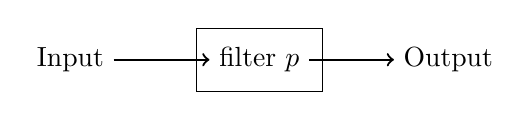
\begin{tikzpicture}[scale=0.8]
      \draw (2, 0) rectangle (4, 1) node (filter) [pos=.5] {filter $p$};
      \draw (0, .5) node (in) {Input}
            (6, .5) node (out) {Output};
      \draw[thick, ->] (in) edge (filter)
                       (filter) edge (out);
      \end{tikzpicture} \\
   \caption{Input: $[x_1, x_2, ..., x_n]$, Output: $[x_1', x_2', ..., x_m']$. and $\forall x_i' \Rightarrow p(x_i')$.}
   \label{fig:filter}
\end{figure}

We can define it in ZF expression:

\be
filter(p, X) = [x_i | x_i \in X, p(x_i)]
\ee

Different from $find$, when there is no element satisfies the predicate, $filter$ returns the empty list. It scans to examine every element one by one:

\be
\begin{array}{rcl}
filter(p,\ \nil) & = & \nil \\
filter(p,\ x:xs) & = & \begin{cases}
  p(x): & x : filter(p, xs) \\
  otherwise: & filter(p, xs) \\
  \end{cases}
\end{array}
\ee

This definition builds the result from right to left. For iterative implementation, if build the result with $append$, it will degrade to $O(n^2)$.

\begin{algorithmic}[1]
\Function{Filter}{$p, L$}
  \State $L' \gets$ NIL
  \While{$L \neq$ NIL}
    \If{$p$(\Call{First}{$L$})}
      \State $L' \gets$ \textproc{Append}($L'$, \Call{First}{$L$}) \Comment{Linear time}
    \EndIf
    \State $L \gets$ \Call{Rest}{$L$}
  \EndWhile
\EndFunction
\end{algorithmic}

The right way is to use $cons$ instead, however, it builds the result in the reversed order. We can further reverse it within linear time (see the exercise). The nature to build result from right indicates that we can define filter in $foldr$. We need define a function $f$ to test an element against the predicate, if OK, prepend to the result:

\be
f(x, A) = \begin{cases}
  p(x): & x : A \\
  otherwise: & A \\
  \end{cases}
\ee

We also need pass the predicate $p$ to $f$. There are actually 3 parameters as $f(p, x, A)$. Filter is defined in $foldr$ with a Curried form of $f$:

\be
filter(p) = foldr((x, A) \mapsto f(p, x, A), \nil)
\ee

We can further simplify it (called $\eta$-conversion\cite{slpj-book-1987}) as:

\be
filter(p) = foldr(f(p), \nil)
\ee

Filter is also a generic concept not only limit to list. We can apply a predicate on any traversable structures to extract the result.

\subsection{Match}
\index{List!matching} \index{List!prefix}
\index{List!suffix} \index{List!infix}

Match is to find a pattern among some structure. Even if we limit to list and string, there are still too many things to cover. We have dedicated chapters about string matching. This section deals with the problem, that given a list $A$, and test if it exits in another list $B$. There are two special cases: to test if $A$ is prefix or suffix of $B$. The $span$ algorithm in (\ref{eq:span}) actually finds a prefix under a certain condition. We can do similar things: to compare each element between $A$ and $B$ from left till meet any different one or reach the end of either list. Define $A \subseteq B$ if $A$ is prefix of $B$:

\be
\begin{array}{rcl}
\nil \subseteq B & = & True \\
(a:as) \subseteq \nil & = & False \\
(a:as) \subseteq (b:bs) & = & \begin{cases}
  a \neq b: & False \\
  a = b: & as \subseteq bs \\
  \end{cases}
\end{array}
\ee

Prefix testing takes linear time as it scans the lists. However, we can not do suffix testing in this way because it is hard to start from the aligned right ends, and scan backwards for lists. This is different from array. Alternatively, we can reverse both lists in linear time, hence change the problem to prefix testing:

\be
A \supseteq B = reverse(A) \subseteq reverse(B)
\ee

With $\subseteq$ defined, we can test if a list is the sub-list of another one. We call it infix testing. The idea is to scan the target list, and repeatedly applying the prefix testing:

\be
\begin{array}{rcl}
infix?(a:as,\ \nil) & = & False \\
infix?(A,\ B) & = & \begin{cases}
  A \subseteq B: & True \\
  otherwise: & infix?(A, B') \\
  \end{cases}
\end{array}
\ee

For the edge case that $A$ is empty, we define empty is infix of any list. Because $\nil \subseteq B$ is always true, it gives the right result. It also evaluates $infix?(\nil, \nil)$ correctly. Below is the corresponding iterative implementation:

\begin{algorithmic}[1]
\Function{Is-Infix}{$A, B$}
  \If{$A = $ NIL}
    \State \Return TRUE
  \EndIf
  \State $n \gets |A|$
  \While{$B \neq$ NIL and $n \leq |B|$}
    \If{$A \subseteq B$}
      \State \Return TRUE
    \EndIf
    \State $B \gets$ \Call{Rest}{$B$}
  \EndWhile
  \State \Return FALSE
\EndFunction
\end{algorithmic}

Because prefix testing runs in linear time, and it is called in the loop of scan. This algorithm is bound to $O(nm)$, where $m, n$ are the length of the two lists respectively. It is an interesting problem to improve this `position by position' scan algorithm to linear time, even when we apply it to arrays. Chapter 13 introduces some smart methods, like the Knuth-Morris-Pratt (KMP) algorithm and Boyer-Moore algorithm. Appendix C introduces another method called suffix-tree.

In a symmetric way, we can enumerate all suffixes of $B$, and check if $A$ is prefix of any of them:

\be
infix?(A, B) = \exists S \in \textit{suffixes}(B), A \subseteq S
\ee

This can be implemented with list comprehension as below example Haskell program:

\begin{Haskell}
isInfixOf a b = (not . null) [ s | s <- tails(b), a `isPrefixOf` s]
\end{Haskell}

Where function \texttt{isPrefixOf} does the prefixing testing, \texttt{tails} generates all suffixes of a given list. We left its implementation as an exercise.

\begin{Exercise}
\Question{Implement the linear time existence testing algorithm.}
\Question{Implement the iterative look up algorithm.}
\Question{Implement the linear time filter algorithm through $reverse$.}
\Question{Implement the iterative prefix testing algorithm.}
\Question{Implement the algorithm to enumerate all suffixes of a list.}
\end{Exercise}

\section{zip and unzip}
\index{List!zip} \index{List!unzip}

The assoc list of paired values is often used as a light weighted dictionary for small set of data. It is easier to build assoc list than tree or heap based dictionary, although the look up performance of assoc list is linear instead of logarithm. In the `$n$-lights' puzzle, we build the assoc list as below:

\[
map(i \mapsto (i, 0),\ [1, 2, ..., n])
\]

More often, we need 'zip' two lists to one. We can define a $zip$ function to do that:

\be
\begin{array}{rcl}
zip(A,\ \nil) & = & \nil \\
zip(\nil,\ B) & = & \nil \\
zip(a:as,\ b:bs) & = & (a, b) : zip(as, bs) \\
\end{array}
\ee

This algorithm works even the two lists have different length. The result length equals to the shorter one. We can even use it to zip infinite lists (under lazy evaluation if both are infinite), for example\footnote{In Haskell: \texttt{zip (repeat 0) [1..n]}}:

\[
zip([0, 0, ...], [1, 2, ..., n])
\]

For a list of words, we can index them with numbers as:

\[
zip([1, 2, ...], [a, an, another, ...])
\]

$zip$ build the result from right. We can also define it with $foldr$. It is bound to $O(m)$ time, where $m$ is the length of the shorter list. When implement the iterative $zip$, the performance will drop to quadratic if using $append$, unless with the reference to the tail position.

\begin{algorithmic}[1]
\Function{Zip}{$A, B$}
  \State $C \gets$ NIL
  \While{$A \neq$ NIL and $B \neq$ NIL}
    \State $C \gets $ \textproc{Append}(C, (\Call{First}{$A$}, \Call{First}{$B$})) \Comment{Linear time}
    \State $A \gets$ \Call{Rest}{$A$}
    \State $B \gets$ \Call{Rest}{$B$}
  \EndWhile
  \State \Return $C$
\EndFunction
\end{algorithmic}

To avoid $append$, we can use 'cons' then reverse the result. However, it can not deal with two infinite lists. In imperative settings, we can also re-use $A$ to store the result (treat it as transform a list of elements to a list of pairs).

We can extend to $zip$ multiple lists to one. Some programming libraries provide, \texttt{zip}, \texttt{zip3}, \texttt{zip4}, ..., till \texttt{zip7}. Sometimes, we don't want to build a list of pairs, but apply a combinator function. For example, given a list of unit prices $[1.00, 0.80, 10.05, ...]$ for fruits: apple, orange, banana, ... When customer has a list of quantities, like $[3, 1, 0, ...]$, means this customer, buys 3 apples, 1 orange, 0 banana, ... Below program generates a payment list:

\[
\begin{array}{rcl}
pays(U,\ \nil) & = & \nil \\
pays(\nil,\ Q) & = & \nil \\
pays(u:us,\ q:qs) & = & (u \cdot q) : pays(us, qs) \\
\end{array}
\]

It is same as the $zip$ function except uses multiply but not 'cons' to combine elements. We can abstract the combinator as a function $f$, and pass it to $zip$ to build a generic algorithm:

\be
\begin{array}{rcl}
zipWith(f, A,\ \nil) & = & \nil \\
zipWith(f, \nil,\ B) & = & \nil \\
zipWith(f, a:as,\ b:bs) & = & f(a, b) : zipWith(f, as, bs) \\
\end{array}
\ee

Here is an example that defines the inner-product (or dot-product)\cite{wiki-dot-product} through $zipWith$:

\be
A \cdot B = sum(zipWith(\cdot, A, B))
\ee

$unzip$ is the inverse operation of $zip$. It converts a list of pairs to two separated lists. Below is its definition with $foldr$ in Curried form:

\be
unzip = foldr((a, b), (A, B) \mapsto (a : A, b : B), (\nil, \nil))
\ee

We fold from a pair of empty lists, break $a, b$ from the pairs and prepend them to the two intermediate lists respectively. We can also use $fst$ and $snd$ explicitly as:

\[
(p, P) \mapsto (fst(p) : fst(P), snd(p) : snd(P))
\]

For the fruits example, suppose the unit price is stored in a assoc list: $U = [(apple, 1.00), (orange, 0.80), (banana, 10.05), ...]$ for lookup, for example $lookup(melon, U)$. The purchase quantity is a assoc list: $Q = [(apple, 3), (orange, 1), (banana, 0), ...]$. How to calculate the total payment? The straight forward way is to extract the unit price and the quantity lists, then compute their inner-product:

\be
pay = sum(zipWith(\cdot, snd(unzip(U)), snd(unzip(Q))))
\ee

As an example, let's see how to use $zipWith$ to define infinite Fibonacci numbers with lazy evaluation:

\be
F = 0 : 1 : zipWith(+, F, F')
\ee

Where $F$ is the infinite list of Fibonacci numbers, starts from 0 and 1. $F'$ is the rest Fibonacci numbers without the first one. From the third, every Fibonacci number is the sum of numbers from $F$ and $F'$ at the same position. Below example program list the first 15 Fibonacci numbers:

\begin{Haskell}
fib = 0 : 1 : zipWith (+) fib (tail fib)

take 15 fib
[0,1,1,2,3,5,8,13,21,34,55,89,144,233,377]
\end{Haskell}

$zip$ and $unzip$ are generic. We can expand to $zip$ two trees, where the nodes contain paired elements from both. When traverse a collection of elements, we can also use the generic $zip$ and $unzip$ to track the path, this is a method to mimic the `parent' reference in imperative implementation (last chapter of \cite{learn-haskell}).

\begin{Exercise}
\Question{Design the iota ($I$) algorithm for below usages:
  \begin{itemize}
  \item $iota(..., n) = [1, 2, 3, ..., n]$;
  \item $iota(m, n) = [m, m + 1, m + 2, ..., n]$, where $m \leq n$;
  \item $iota(m, m+a, ..., n) = [m, m + a, m + 2a, ..., n]$;
  \item $iota(m, m, ...) = repeat(m) = [m, m, m, ...]$;
  \item $iota(m, ...) = [m, m + 1, m + 2, ... ]$.
  \end{itemize}
  The last two cases are about infinite list. One possible implementation is through streaming and lazy evaluation (\cite{SICP} and \cite{learn-haskell}).}

\Question{Implement the linear time imperative $zip$ algorithm}

\Question{Define $zip$ with $foldr$.}

\Question{For the fruits example, suppose the quantity assoc list only contains the items with none-zero quantity. i.e. instead of
\[
Q = [(apple, 3), (banana, 0), (orange, 1), ...]
\]
but
\[
Q = [(apple, 3), (orange, 1), ...]
\]
because customer does not buy banana. Design a program to calculate the total payment.}

\Question{Implement $lastAt$ with $zip$.}

\end{Exercise}

\section{Further reading}
List is the fundamental thing to build more complex data structures and algorithms particularly in functional settings. We introduced elementary algorithms to construct, access, update, and transform list; how to search, filter data, and compute atop list. Although most programming environments provide pre-defined tools and libraries to support list, we should not simply treat them as black-boxes. Rabhi and Lapalme introduce many functional algorithms about list in \cite{algo-fp}. Haskell library provides detailed documentation about basic list algorithms. There are materials provide good examples of folding, especially in \cite{fp-pearls}. It also introduces about the {\em fold fusion law}.

\begin{Exercise}

\Question{Design algorithm to remove the duplicated elements in a list. For imperative implementation, the elements should be removed in-place. The original element order should be maintained. What is the complexity of this algorithm? How to simplify it with additional data structure?}

\Question{List can represent decimal non-negative integer. For example 1024 as list is $4 \rightarrow 2 \rightarrow 0 \rightarrow 1$. Generally, $n = d_m...d_2d_1$ can be represented as
$d_1 \rightarrow d_2 \rightarrow ... \rightarrow d_m$. Given two numbers $a$, $b$ in list form. Realize arithmetic operations such as add and subtraction.}

\Question{In imperative settings, a circular linked-list is corrupted, that some node points back to previous one, as shown in figure \ref{fig:circular-list}. When traverse, it falls into infinite loops. Design an algorithm to detect if a list is circular. On top of that, improve it to find the node where loop starts (the node being pointed by two precedents).}

\end{Exercise}

\begin{figure}[htbp]
\centering
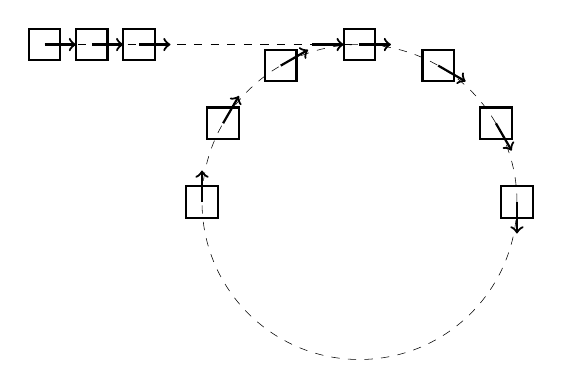
\begin{tikzpicture}[scale=2]
  % trace
  \draw[dashed, very thin] (-2cm, 1cm) -- (0, 1cm);
  \draw[dashed, very thin] (0,0) circle [radius=1cm];

  % leading nodes
  \foreach \x in {-2, -1.7, ..., -1.4} {
    \draw[thick] (\x cm, 1cm) +(-0.1, -0.1) rectangle ++(0.1, 0.1);
    \draw[thick, ->] (\x cm, 1cm) -- +(0.2, 0);
  }

  % cricular starting points
  \draw[thick, ->] (-0.3cm, 1cm) -- (-0.1cm, 1cm);

  % circular nodes
  \foreach \deg/\rot in {90/0, 60/-30, 30/-60, 0/-90, 180/90, 150/60, 120/30} {
    \draw[thick] (\deg : 1cm) +(-0.1, -0.1) rectangle ++(0.1, 0.1);
    \draw[thick, ->] (\deg : 1cm) -- +(\rot : 0.2);
  }
\end{tikzpicture}
\caption{A circular linked-list}
\label{fig:circular-list}
\end{figure}

\ifx\wholebook\relax \else
\begin{thebibliography}{99}

\bibitem{fp-pearls}
Richard Bird. ``Pearls of Functional Algorithm Design''. Cambridge University Press; 1 edition (November 1, 2010). ISBN: 978-0521513388

\bibitem{slpj-book-1987}
Simon L. Peyton Jones. ``The Implementation of Functional Programming Languages''. Prentice-Hall International Series in Computer Since. Prentice Hall (May 1987). ISBN: 978-0134533339

\bibitem{moderncxx}
Andrei Alexandrescu. ``Modern C++ design: Generic Programming and Design Patterns Applied''. Addison Wesley February 01, 2001, ISBN 0-201-70431-5

\bibitem{mittype}
Benjamin C. Pierce. ``Types and Programming Languages''. The MIT Press, 2002. ISBN:0262162091

\bibitem{unplugged}
Xinyu LIU. ``Isomorphism -- mathematics of programming''. 2020. \url{https://github.com/liuxinyu95/unplugged}

\bibitem{SICP}
Harold Abelson, Gerald Jay Sussman, Julie Sussman. ``Structure and Interpretation of Computer Programs, 2nd Edition''. MIT Press, 1996, ISBN 0-262-51087-1

\bibitem{okasaki-book}
Chris Okasaki. ``Purely Functional Data Structures''. Cambridge university press, (July 1, 1999), ISBN-13: 978-0521663502

\bibitem{algo-fp}
Fethi Rabhi, Guy Lapalme. ``Algorithms: a functional programming approach''. Second edition. Addison-Wesley, 1999. ISBN: 0201-59604-0

\bibitem{learn-haskell}
Miran Lipovaca. ``Learn You a Haskell for Great Good! A Beginner's Guide''. No Starch Press; 1 edition April 2011, 400 pp. ISBN: 978-1-59327-283-8

\bibitem{erlang}
Joe Armstrong. ``Programming Erlang: Software for a Concurrent World''. Pragmatic Bookshelf; 1 edition (July 18, 2007). ISBN-13: 978-1934356005

\bibitem{wiki-tail-call}
Wikipedia. ``Tail call''. \url{https://en.wikipedia.org/wiki/Tail_call}

\bibitem{sgi-stl-transform}
SGI. ``transform''. \url{http://www.sgi.com/tech/stl/transform.html}

\bibitem{poj-drunk-jailer}
ACM/ICPC. ``The drunk jailer.'' Peking University judge online for ACM/ICPC. \url{http://poj.org/problem?id=1218}.

\bibitem{Haskell-wiki}
Haskell wiki. ``Haskell programming tips''. 4.4 Choose the appropriate fold. \url{http://www.haskell.org/haskellwiki/Haskell_programming_tips}

\bibitem{wiki-dot-product}
Wikipedia. ``Dot product''. \url{http://en.wikipedia.org/wiki/Dot_product}

\end{thebibliography}

\expandafter\enddocument
\fi


\input{fdl-1.3.tex}

\printindex

\end{document}
